\documentclass[12pt,a4paper,openright,twoside]{book}
\usepackage[utf8]{inputenc}
\usepackage{phd-thesis}
\usepackage{code-lstlistings}
\usepackage{notes}
\usepackage{shortcuts}

%----------------------------------------------------------------------------------------
% Packages and definitions required by the integrated papers (Chapters 3--5)
%----------------------------------------------------------------------------------------
\usepackage{amssymb}    % Papers 2, 4 (symbols)
\usepackage{array}      % Paper 3 supplementary tables (>{\raggedright}p{..} columns)
\usepackage{multirow}   % Papers 2, 3, 6 (multi-row table cells)
\usepackage{booktabs}   % Papers 3, 6 (\toprule, \midrule, \bottomrule)
\usepackage{longtable}  % Paper 1, Table 1 (99 rows over several pages)
\usepackage{pdflscape}  % Paper 1, Table 1 (landscape pages)
\usepackage{subcaption} % Paper 6 (subfigure environment)
\usepackage{placeins}   % \FloatBarrier at the end of each paper (keeps floats within their paper)
\usepackage{caption}    % consistent table caption styling
\captionsetup[table]{font=small,labelfont=bf,skip=6pt}
% Paper 6 uses the column types and table width of the Elsevier cas-common.sty (definitions copied from it)
\newcolumntype{L}{@{\extracolsep{\fill}}l}
\newcolumntype{C}{@{\extracolsep{\fill}}c}
\newlength{\tblwidth}\AtBeginDocument{\setlength{\tblwidth}{\textwidth}}
% The papers' own sections become \subsection within each chapter; number one more level so that the
% papers' internal cross-references (e.g. "Section~\ref{...}") resolve to a numbered unit.
\setcounter{secnumdepth}{3}

\mainlinespacing{1.241} % line spacing in mainmatter, comment to default (1)

\begin{document}
	
\frontmatter
%!TeX root = phd-thesis.tex
\title{Data-centric Approaches for Trustworthy AI Systems}
\author{Alberto Marfoglia}
\date{\today}

\newgeometry{margin=0.8in}
\begin{titlepage}
	\begin{center}
		% \vspace*{0.2cm}

		\large
		\textbf{ALMA MATER STUDIORUM -- UNIVERSITÀ DI BOLOGNA \\ DISI Dipartimento di Informatica: Scienza e Ingegneria}
		\\
		\noindent\hrulefill
		\vspace{0.4cm}

		\Large
		Dottorato di Ricerca in \\
		Computer Science and Engineering

		\vspace{0.4cm}

		Ciclo XXXIX

		\vspace{0.4cm}

		Settore Scientifico Disciplinare: INF/01, Informatica

		Settore Concorsuale: 01/B1

		\Huge
		\vspace{3cm}
		\textbf{
			Semantic and Data-Centric Approaches for Trustworthy AI in Healthcare
		}

		{\Large{
		\vspace{3cm}

		\textit{Candidato:\\}
		\centering
		Dott. Alberto Marfoglia}
		\\}
		\large
		\vspace{2.5cm}
		\begin{minipage}[t]{0.64\textwidth}
			\begin{flushleft}
				%\textit{Coordinatrice Dottorato:}
				%\\
				%\textbf{Prof.ssa Paola Salomoni}
			\end{flushleft}
		\end{minipage}
		\begin{minipage}[t]{0.34\textwidth}
			\begin{flushright}
				\textit{Supervisore:}
				\\
				\textbf{Prof.ssa} \textbf{Antonella Carbonaro}
				\\
				%\vspace{0.4cm}
				%\textit{Co-supervisore:}
				%\\
				%\textbf{Prof.} \textbf{Vittorio Maniezzo}
			\end{flushright}

		\end{minipage}\\

		\vfill
		\noindent\hrulefill
		\vspace{0.3cm}
		\Large

		Esame finale anno 2027
	\end{center}
\end{titlepage}
\restoregeometry

\begin{abstract}	
Max 2000 characters, strict.
\end{abstract}

\begin{dedication} % this is optional
Optional. Max a few lines.
\end{dedication}

\begin{acknowledgements} % this is optional
Optional. Max 1 page.
\end{acknowledgements}

%----------------------------------------------------------------------------------------
\tableofcontents   
\listoffigures     % (optional) comment if empty
%\lstlistoflistings % (optional) comment if empty
%----------------------------------------------------------------------------------------

\mainmatter

%----------------------------------------------------------------------------------------

\chapter{Introduction}
\label{chap:introduction}

The increasing digitalization of society is transforming the way information is produced, exchanged, and used \cite{oecd_progress_2026, oecd_scaling_2026}. The growing connectivity between people, devices, and digital services, together with the availability of increasingly large volumes of data and computational resources, has enabled the development of technologies capable of supporting tasks that were previously difficult or impossible to perform \cite{oecd_collective_2024}. Among these technologies, Artificial Intelligence (AI) has emerged as one of the principal drivers of contemporary digital transformation, with applications spanning domains such as healthcare, transportation, finance, manufacturing, and scientific research \cite{hamon_robustness_2020, oecd_progress_2026, annoni_artificial_2018}.

However, the availability of large volumes of data does not automatically translate into reliable information or effective AI systems \cite{peters_dikw_2025}. Data originating from different organizations, applications, devices, and processes may differ in structure, quality, and semantics \cite{oecd_interoperability_2026}. Consequently, the ability to access, integrate, interpret, and reuse data becomes a fundamental prerequisite for exploiting their value \cite{chamola_review_2023}.

This challenge is particularly relevant for AI systems because contemporary Machine Learning (ML) approaches derive computational models from data rather than relying exclusively on explicitly encoded rules \cite{chamola_review_2023}. The resulting systems can achieve remarkable predictive performance, but their behavior is inherently dependent on the characteristics of the data used throughout their lifecycle \cite{oecd_collective_2024}. Consequently, issues concerning data representation and governance are not merely peripheral concerns but can directly affect the behavior and reliability of the resulting AI systems \cite{oecd_collective_2024, zha_data-centric_2025, oecd_scaling_2026}.

Moreover, to achieve the effective adoption of AI in society, humans must remain at the center of this technological evolution. Cutting-edge solutions should support human autonomy and establish a relationship of trust \cite{kaur_trustworthy_2022}. In general terms, the National Institute of Standards and Technology defines trust as \emph{“the confidence one element has in another, that the second element will behave as expected”} \cite{boyens_supply_2015}.

The challenge therefore extends beyond developing increasingly sophisticated AI models \cite{zha_data-centric_2025, kaur_trustworthy_2022}. This thesis investigates the role of data-centric engineering in the development of Trustworthy AI systems. In particular, it examines how semantic approaches can make two steps explicit and machine-actionable: the transformation of heterogeneous data into structured information and computable knowledge, and the connection of that knowledge to AI models. The aim is to enable AI-supported analysis that can inform human decision-making. Healthcare is adopted as the application domain of this research. It represents a particularly relevant setting for this investigation, as it is a fundamental component of civil society in which technological advancements must remain reliable and firmly oriented towards serving individuals and promoting their well-being.

\section{Data-Centricity in the Age of AI}

AI is expected to profoundly reshape the social and economic landscape of contemporary societies, while stimulating innovation across a wide range of domains~\cite{annoni_artificial_2018}. It encompasses a broad family of computational approaches designed to enable machines to perform tasks that typically require cognitive capabilities, such as perception, prediction, reasoning, learning, and decision-making~\cite{hamon_robustness_2020}. In recent years, advances in AI have been driven particularly by ML, which enables computational models to infer patterns and relationships from data rather than relying exclusively on manually specified rules~\cite{chamola_review_2023}. The generality of these approaches allows similar underlying principles to be applied to substantially different problems, provided that suitable data are available~\cite{annoni_artificial_2018}.

These considerations motivate a shift in attention from the exclusive optimization of models towards the systematic engineering of the data on which AI systems depend~\cite{zha_data-centric_2025}. This shift has given rise to the concept of \emph{Data-Centric AI}, which places data at the center of the AI development lifecycle. It is important, however, to distinguish \emph{data-centric} from \emph{data-driven}. The latter primarily refers to the use of data as the basis for developing computational models, whereas a data-centric approach goes further by treating data themselves as engineering artifacts whose quality, structure, representation, documentation, and lifecycle require systematic attention~\cite{zha_data-centric_2025}. This perspective does not imply a replacement of model-centric approaches. Rather, data-centric and model-centric practices are complementary and jointly contribute to the development of reliable and effective AI systems.

%Besides training data, well-designed inference data, the input used in the inference phase of AI systems for making predictions, has facilitated the initial recognition of numerous critical issues in AI and unlocked new model capabilities \cite{zha_data-centric_2025}.

As the volume, variety, and velocity of available data continue to increase, manual approaches alone become increasingly difficult to sustain. Consequently, data-centric AI also requires automated methods to support and streamline the data lifecycle~\cite{zha_data-centric_2025}. This lifecycle comprises multiple stages, including \emph{Training Data Development} and \emph{Data Maintenance}~\cite{zha_data-centric_2025}.

\paragraph{Training Data Development} concerns the collection, integration, and preparation of data for AI model development~\cite{zha_data-centric_2025}. This process can require substantial engineering effort; a frequently cited estimate suggests that it accounts for approximately 80\% of data scientists' work~\cite{press_cleaning_2020}. It comprises (a) \emph{Data collection}, which gathers data from relevant sources and requires domain knowledge to determine what should be collected and how it should be represented; (b) \emph{Data integration}, which combines data from multiple sources into a unified representation by aligning attributes and transforming source-specific values; and (c) \emph{Data preparation}, which cleans and transforms the resulting data into a form suitable for model development.

\paragraph{Data Maintenance} recognizes that data are continuously generated, updated, and reused in operational environments~\cite{zha_data-centric_2025}. It therefore comprises (a) \emph{Data understanding}, which supports the interpretation and assessment of complex datasets through activities such as summarization and visualization, enabling stakeholders to evaluate data characteristics, provenance, limitations, and suitability for their intended use; (b) \emph{Data storage and retrieval}, which provide the scalable infrastructure required to make data available to AI systems as data volumes and generation rates increase; and (c) \emph{Data quality assurance}, which involves the continuous assessment and improvement of data quality. It may consider objective dimensions, such as accuracy, timeliness, consistency, and completeness, as well as human-centered dimensions, including trustworthiness, understandability, and accessibility.


%\paragraph{Data understanding} is equally important because real-world datasets are often large, heterogeneous, and difficult to interpret. A comprehensive understanding of the characteristics, provenance, limitations, and intended use of data is necessary to assess their suitability for a particular task and to identify potential sources of error or bias~\cite{zha_data-centric_2025}. Such understanding should extend beyond the data themselves to the contexts in which they were collected, processed, and intended to be used. This is particularly important when data are subsequently employed in environments that differ from those in which they were originally collected.

%\paragraph{Data quality assurance} concerns the continuous assessment and maintenance of data quality throughout the lifecycle of an AI system. In real-world settings, both data sources and the infrastructures used to process them are subject to frequent and continuous change. Consequently, it is not sufficient to produce high-quality training or inference data at a single point in time; their quality must be monitored and maintained as the underlying data and operational environment evolve~\cite{zha_data-centric_2025}. This requires appropriate metrics and evaluation procedures for characterizing different dimensions of data quality. Importantly, data quality cannot be understood solely through technical measures. It also encompasses human-centered dimensions, including trustworthiness, understandability, and accessibility~\cite{zha_data-centric_2025}. Trustworthiness concerns the reliability and accuracy of information provided by a data source; understandability concerns the extent to which users can comprehend the collected data; and accessibility concerns the ability of relevant users to access and effectively use the data.

Taken together, these activities illustrate that data in AI systems are not merely passive inputs to computational models. They are artifacts that must be acquired, transformed, documented, validated, monitored, maintained, and interpreted throughout their lifecycle. Data management is therefore a fundamental component of Trustworthy AI, motivating principles and practices for the appropriate storage, management, and use of data~\cite{hamon_robustness_2020}. Building on these principles, data and AI governance are gaining increasing prominence as mechanisms for ensuring that the design, development, deployment, and ongoing management of AI systems remain aligned with the values, responsibilities, and expectations of organizations and society~\cite{hamon_robustness_2020}.

\section{From Data to AI Governance}

The central role of data in contemporary AI systems makes their management an essential component of responsible AI development. This has motivated principles and practices for \emph{Data Governance}, aimed at ensuring that data are appropriately managed throughout their lifecycle according to requirements concerning quality, accountability, security, privacy, and lawful use~\cite{hamon_robustness_2020}. In the European context, the General Data Protection Regulation (GDPR) establishes a comprehensive framework for the processing of personal data~\cite{data_protection_working_party_article29_nodate}. Its provisions are particularly relevant to AI systems that support or automate decisions concerning individuals, where they raise questions of transparency, interpretability, and the ability of data subjects to obtain an explanation of, and contest, such decisions~\cite{panigutti_role_2023,kaminski_right_2019}.

\emph{AI Governance} extends these concerns from the data to the systems that process them and to the decisions resulting from their operation~\cite{hamon_robustness_2020}. The EU AI Act reflects this extension: it adopts a risk-based approach, prohibiting systems that present unacceptable risks and requiring high-risk systems to be designed so that users can interpret their output and use them appropriately~\cite{oecd_collective_2024,corbucci_semantic_2023}. Notably, the Act does not prohibit black-box models or prescribe specific explanation techniques; it frames transparency primarily as an obligation to provide appropriate information and documentation about the system~\cite{panigutti_role_2023,panigutti_co-design_2023}. Trustworthiness, in this view, cannot be achieved through model performance alone, but requires coordinated attention to the data, the technical system, its documentation, and the humans involved in its operation~\cite{panigutti_role_2023,oecd_collective_2024}. Of these, the explicit specification of data, of the processes that transform them, and of the way they are used by models is the aspect most directly relevant to this thesis.

\section{Trustworthy AI}\label{sec:trustworthy-ai}

As anticipated in the previous section, the objective is not only to ensure that the underlying data are appropriately managed, but also that AI systems operate in accordance with legal requirements, ethical principles, technical constraints, and societal expectations \cite{hamon_robustness_2020}. This shift from Data Governance to AI Governance is reflected in the increasing international and European attention devoted to \emph{Trustworthy AI}. The need for trustworthy systems arises from the observation that technical performance alone is insufficient to determine whether an AI system is appropriate for deployment~\cite{kaur_trustworthy_2022}. An AI system may achieve high predictive accuracy yet remain unsuitable for a specific context, such as healthcare, due to biased data, inadequate privacy protection, limited robustness, lack of transparency, or insufficient mechanisms for human intervention
\cite{kaur_trustworthy_2022, oecd_progress_2026, li_trustworthy_2023}.

Trustworthy AI therefore extends the assessment of AI systems beyond predictive performance. Several organizations and research communities have proposed principles and frameworks for Trustworthy AI~\cite{european_commission_ethics_nodate,lekadir_future-ai_2025, oecd_oecd_2019,unesco_recommendation_2022}, with an emerging convergence around dimensions including transparency and explainability \cite{kaur_trustworthy_2022}. From this perspective, trustworthiness is not a single technical property that can be added to an AI system after its development. Rather, it results from the interaction of multiple properties that must be considered throughout the AI lifecycle.

\paragraph{The EU framework.}
The European Commission's \emph{Ethics Guidelines for Trustworthy AI} provide a comprehensive framework for the development, deployment, and use of trustworthy AI systems~\cite{european_commission_ethics_nodate}. According to these guidelines, AI systems should be (a) \emph{lawful}, by respecting applicable laws and regulations; (b) \emph{ethical}, by adhering to ethical principles and values; and (c) \emph{robust}, both from a technical perspective and with regard to their social environment.

To operationalize these principles, the guidelines identify seven key requirements for Trustworthy AI~\cite{european_commission_ethics_nodate,kaur_trustworthy_2022}: (1) \emph{human agency and oversight}, ensuring that AI systems support human autonomy and allow for appropriate human intervention; (2) \emph{technical robustness and safety}, ensuring reliable and safe operation, including under unexpected conditions or external disturbances; (3) \emph{privacy and data governance}, ensuring the protection of personal data and compliance with applicable data protection requirements; (4) \emph{transparency}, providing relevant information about the system's capabilities, limitations, and operation to enable stakeholders to appropriately understand and use its outputs; (5) \emph{diversity, non-discrimination, and fairness}, preventing unjustified discrimination and accounting for the diversity of individuals and groups affected by AI systems; (6) \emph{societal and environmental well-being}, ensuring that AI systems contribute positively to society while avoiding disproportionate societal or environmental harms; and (7) \emph{accountability}, establishing appropriate mechanisms for assigning responsibility for the development, deployment, operation, and outcomes of AI systems.

\paragraph{The role of data in trust.}
The seven requirements of the EU framework highlight that trustworthiness is a system-level property. At the same time, several of these requirements are directly or indirectly shaped by how data are collected, represented, transformed, documented, and maintained~\cite{kaur_trustworthy_2022}. Privacy and data governance explicitly concern the management of data, but their influence extends beyond this requirement. Technical robustness depends, among other factors, on the quality and suitability of the data used for training and operation. Fairness can be compromised by biases and under-representation in datasets, while transparency and accountability can be strengthened when the provenance, meaning, transformations, and intended uses of data can be established and communicated. Similarly, effective human oversight relies on the availability of sufficient contextual information to enable users to appropriately assess and interpret AI outputs~\cite{guidotti_survey_2019}.

Building on these observations, this thesis adopts the position that data-centricity is a necessary, though not sufficient, enabler of Trustworthy AI. This position is a premise of the thesis, grounded in the literature discussed above, rather than a hypothesis it tests; what the thesis investigates is how data-centric engineering can act as such an enabler, and which requirements of Trustworthy AI it can support. The underlying argument is that trustworthiness cannot be reliably built on data that are poorly understood, inaccessible, or connected to models in ways that cannot be inspected. This perspective calls for a wider interpretation of the data-centric paradigm. Data engineering should not be limited to improving the statistical properties of the datasets used for model training; it should also address how data are represented, how their meaning is made explicit, and how they are connected to the models that use them.

\paragraph{Explainable AI.}
Among the requirements of Trustworthy AI, transparency and explainability are particularly relevant to the relationship between AI systems and their human users. The field of Explainable AI (XAI) encompasses technical approaches for designing interpretable models and generating explanations~\cite{guidotti_survey_2019}, methodologies for evaluating explanations~\cite{lekadir_future-ai_2025}, and contributions from the social sciences concerning the nature and role of explanations~\cite{miller_explanation_2019}. There is no universally accepted formal definition of an \emph{explanation}~\cite{miller_explanation_2019}, and what constitutes an adequate explanation depends on the application, the intended user, and the purpose for which it is required~\cite{murdoch_interpretable_2019}. This thesis does not develop or evaluate explanation methods. Its relevance to explainability is more indirect: explanations of model behavior are ultimately interpreted in terms of the data and domain concepts on which a model operates, and explicit semantic representations of those data and concepts can provide context through which explanations become meaningful~\cite{corbucci_semantic_2023,panigutti_role_2023}.

\section{AI in Healthcare}
\label{ai_in_healthcare}

The healthcare sector represents a particularly relevant context for investigating the opportunities and challenges associated with AI. Healthcare is not only a fundamental component of modern societies but also a complex socio-technical ecosystem involving diverse professions, processes, and practices that rely on the production and exchange of large volumes of information. Consequently, technological progress in healthcare cannot be evaluated solely in terms of computational performance: the quality of care is closely connected to the quality, availability, and interoperability of the information on which clinical and organizational processes depend. AI systems must operate within this complex environment, where their outputs can have significant consequences for human health and well-being. These characteristics make healthcare a particularly demanding and consequential setting for investigating the data-centric foundations of Trustworthy AI.

\paragraph{Digital transformation and system pressures.}
Healthcare is undergoing a profound digital transformation driven by the increasing availability of health data and the adoption of technologies such as AI, the Internet of Things (IoT), and wearable devices~\cite{oecd_progress_2026}. Clinical information already accounts for approximately 30\% of global data, and its volume continues to grow rapidly~\cite{thomason_data_2024}. The healthcare sector itself represents a substantial economic domain, with global expenditure estimated at approximately USD 8.3 trillion~\cite{thomason_data_2024}. At the same time, IoT technologies are expected to generate up to USD 1.8 trillion in economic value by 2030~\cite{seixas-lopes_musculoskeletal_2024}, while the wearable medical device market, valued at USD 14.4 billion in 2020, has been projected to grow at an annual rate of 18.9\%~\cite{thomason_data_2024}. Finally, it is projected that the economic value of the AI market will grow from USD 183 billion in 2023 to USD 995 billion in 2028, a more than fivefold increase~\cite{oecd_collective_2024}.

The relevance of this transformation is further reinforced by the structural pressures faced by healthcare systems. Across the European Union, healthcare expenditure represented approximately 10.4\% of Gross Domestic Product (GDP) in 2022, while healthcare spending increased by approximately 39.9\% between 2014 and 2022 \cite{oecd_progress_2026}. At the same time, demographic aging is increasing the demand for healthcare services: people aged 65 years and over represented approximately 21\% of the European population in 2023 and are projected to account for approximately 29\% by 2050 \cite{oecd_progress_2026}. These demographic and economic trends are accompanied by workforce pressures, with an OECD projection estimating a potential shortage of approximately 3.5 million health professionals by 2030 \cite{oecd_progress_2026}. In this context, AI is increasingly considered not merely as a technological innovation, but as an enabler for new models of care.

\paragraph{AI opportunities.}

The potential impact of AI in healthcare extends across the entire care pathway \cite{oecd_progress_2026}. Estimates suggest that AI could automate or substantially support activities corresponding to up to 36\% of tasks performed in health and social care \cite{kumar_chebrolu_smart_2020}. Such applications could reduce the burden of repetitive administrative and analytical activities, allowing healthcare professionals to devote more attention to patient-centered tasks \cite{oecd_progress_2026, hamon_robustness_2020}. Beyond task automation, the integration of predictive models with technologies such as wearable devices, remote monitoring, and Digital Twins may support more personalized and preventive approaches to care \cite{oecd_progress_2026}.

AI may also contribute directly to clinical decision support. Recent assessments suggest that AI could address approximately 20\% of clinical needs in the coming years~\cite{gonzalez-gonzalo_trustworthy_2022}. It may further help to reduce medical errors due to miscommunication, estimated at 30\% of all errors~\cite{european_alliance_for_access_to_safe_medicines_medication_2022}, and to unlock value from the estimated 97\% of health data that remain unused for decision-making~\cite{oecd_collective_2024}. This gap highlights a central paradox of digital healthcare: \emph{the availability of data is increasing rapidly, while the capacity to transform those data into usable information and actionable knowledge remains comparatively limited}.

Examples of potential applications include (1) \emph{empowering individuals and personalizing care} \cite{oecd_collective_2024}: AI can provide insights into personal health data, facilitate understanding of medical records and healthcare systems, and support informed care decisions \cite{marfoglia_towards_2025,krumholz_big_2014,topol_high-performance_2019}, potentially improving health outcomes, reducing costs, and increasing patient satisfaction \cite{hibbard_what_2013}; (2) \emph{streamlining processes and enhancing decision-making}: AI can reduce clinicians' administrative burden, potentially freeing 10--30\% of their time for patient care, and support evidence-based practice by identifying relevant scientific literature \cite{shanafelt_potential_2016,oecd_collective_2024}; and (3) \emph{advancing drug discovery}: AI can accelerate the identification of promising drug candidates while reducing the resources required for early-stage discovery, as demonstrated by the identification of 240 potential antibiotics from over 7,000 candidates in approximately two hours \cite{liu_deep_2023}.

\section{Research Questions}
\label{sec:research_questions}

\paragraph{Research problem.}
The preceding sections highlight a fundamental problem: despite the growing availability of data and increasingly capable AI methods, integrating these resources into reliable and reusable AI workflows remains challenging. The challenge does not arise from the absence of data standards, semantic technologies, or AI models considered in isolation. Rather, it concerns the connections required to transform heterogeneous source data into standardized representations, make their meaning explicit, and connect them to the computational models that consume them. In current practice, these connections are frequently implicit, opaque, or dependent on costly manual configurations, making them difficult to inspect, reuse, and transfer across settings.

\paragraph{Research gap.}
The research problem can be further specified through three interfaces that remain insufficiently addressed by existing approaches. First, the adoption of data standards does not by itself ensure that heterogeneous data are mapped, transformed, and validated consistently across source environments. Implementation practices remain variable, and transformation processes often depend on implementation-specific logic or manual validation, which limits their reproducibility and reuse across contexts~\cite{oecd_interoperability_2026,williams2023standardized,simon2024metadata}. Second, structural harmonization does not necessarily make the meaning and relationships of data, or the input requirements of computational models, explicit in a machine-interpretable form. This limits the ability to connect domain information with computational capabilities~\cite{rathee_semantic_2025,xhani_role_2025}. Moreover, when semantic representations are used as input to learning methods, their design is often treated as a neutral serialization choice, and its influence on downstream performance is rarely examined explicitly. Third, even when structured data and semantic resources are available, connecting them operationally with computational models remains challenging: matching model requirements to instance-specific data and invoking models within continuously updated environments typically requires manual integration effort~\cite{felicetti_knowledge_2025,Katsoulakis2024}.

\paragraph{Research aim.}
This thesis investigates how semantic, data-centric engineering can transform implicit connections into explicit, machine-actionable specifications. It follows a progression from heterogeneous data to interoperable information, from information to computable knowledge, and from knowledge to AI-supported analysis. Along this progression, it examines how such specifications contribute to fulfilling selected requirements of Trustworthy AI. The underlying expectation is threefold: interoperable and verifiable representations can enhance the reliability and reusability of AI inputs; explicit semantics can make data and model dependencies traceable and inspectable; and the integration of computational environments with their application context can facilitate stakeholder oversight and the interpretation of AI-generated results.

\paragraph{Research questions.}
Accordingly, the thesis addresses the following main research question, investigated in the healthcare domain:

\begin{quote}
\textbf{MRQ:} How can semantic, data-centric engineering make the dependencies between heterogeneous data and AI models explicit and machine-actionable, and how does this support selected requirements of Trustworthy AI?
\end{quote}

\noindent The main question is decomposed into three sub-questions. Each corresponds to one of the interfaces identified above and to one of the methodological stages described in Chapter~\ref{chap:research_overview}:

\begin{enumerate}

\item \textbf{RQ1} (\emph{Harmonization and Structuring}): How can heterogeneous health data be harmonized into interoperable, traceable, and verifiable standard-based representations for AI workflows?

\item \textbf{RQ2} (\emph{Semantic Enrichment}): How can semantic representations make the meaning of data and the interface requirements of AI models transparent, and how does making this meaning explicit affect the use of data in predictive tasks?

\item \textbf{RQ3} (\emph{Inference and Reasoning}): How can semantically represented knowledge and AI models be integrated within a virtual replica to support human decision-making?

\end{enumerate}

\section{Thesis Outline}
\label{sec:thesis_outline}

This thesis is organized as a collection of six published contributions, framed by chapters that introduce them and draw them together. The remainder of the thesis is structured as follows.

\begin{itemize}

\item \textbf{Chapter~\ref{chap:research_overview}} presents the research philosophy of the thesis. It introduces the conceptual framework that connects the contributions, namely the DIKW model, the data-centric methodology, and the principles of Trustworthy AI. For each of the three methodological stages, it provides the necessary background and summarizes the associated contributions.

\item \textbf{Chapter~\ref{chap:harmonization_structuring}} addresses RQ1 and contains the contributions on \emph{Harmonization and Structuring}: a systematic review of how health data standards are adopted in practice (Paper~1), and a modular pipeline for transforming heterogeneous clinical data into a standardized representation (Paper~2).

\item \textbf{Chapter~\ref{chap:semantic_enrichment}} addresses RQ2 and contains the contributions on \emph{Semantic Enrichment}: an ontology-driven representation of clinical event data and its use in graph-based prediction (Paper~3), and a formal description of the interfaces of AI models (Paper~4).

\item \textbf{Chapter~\ref{chap:inference_reasoning}} addresses RQ3 and contains the contributions on \emph{Inference and Reasoning}: an architecture for patient Digital Twins backed by Personal Knowledge Graphs (Paper~5), and its implementation with the automated integration of AI models (Paper~6).

\item \textbf{Chapter~\ref{chap:conclusions}} answers the research questions, discusses the implications of the findings for Trustworthy AI, and outlines directions for future research.

\end{itemize}

%\noindent The six papers are reproduced as published. Each therefore retains its own introduction, related work, and notation, and some overlap between them and with the framing chapters is to be expected.


\chapter{Research Philosophy and Overview}
\label{chap:research_overview}

This chapter presents the research philosophy that underpins the thesis and provides an overview of how its individual contributions are connected. Rather than considering the investigated technologies as isolated solutions, the thesis interprets them as successive methodological interventions along a broader progression from heterogeneous data towards actionable knowledge and AI-supported decision-making. This perspective, summarized in Figure~\ref{fig:research_perspective}, combines three complementary dimensions: (1) the Data--Information--Knowledge--Wisdom (DIKW) model~\cite{peters_dikw_2025}, adopted as a conceptual framework, describes the transformation through which diverse observations are progressively converted into information, knowledge, and ultimately actionable insights; (2) the data-centric methodology identifies the principal intervention points through which these transformations can be operationalized, namely \emph{Harmonization and Structuring}, \emph{Semantic Enrichment}, and \emph{Inference and Reasoning}; and (3) Trustworthy AI provides a cross-cutting perspective through which the resulting methods and systems can be interpreted. 
This conceptualization provides the basis for organizing the contributions presented in the following chapters.

\begin{figure}[t]
    \centering
    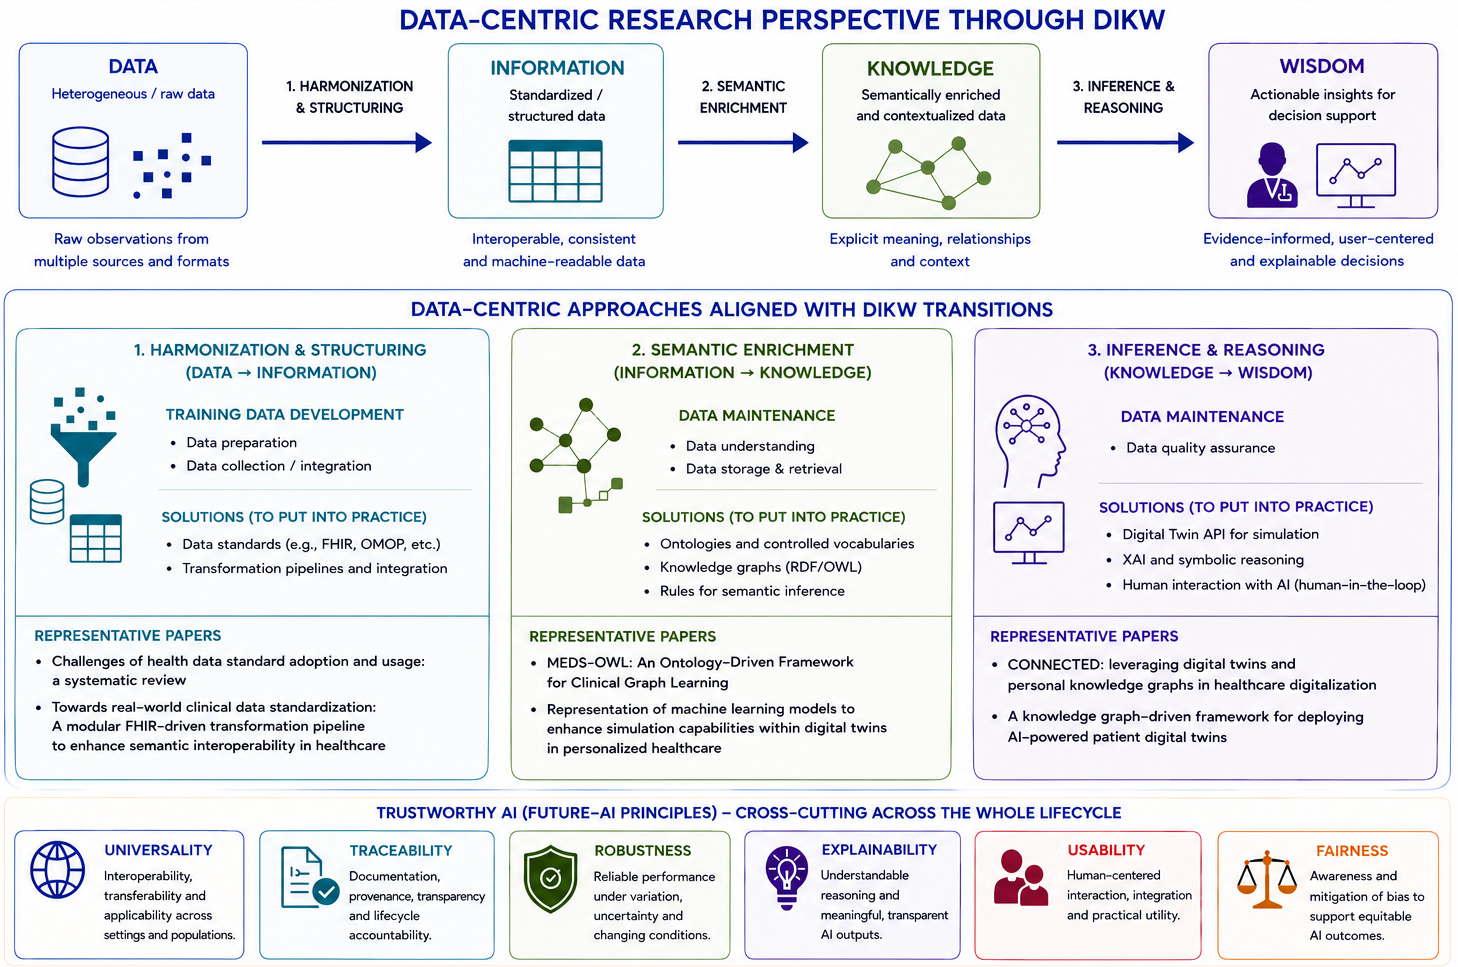
\includegraphics[width=\textwidth]{figures/fig1.png}
    \caption{Data-centric research perspective through the DIKW progression. The three methodological stages represent the principal transitions investigated in the thesis, while Trustworthy AI principles provide a cross-cutting perspective across the data and AI lifecycle.}
    \label{fig:research_perspective}
\end{figure}


\section{Research Methodology}
\label{sec:research_methodology}

Methodologically, this thesis adopts a design-oriented research approach. With the exception of the systematic literature review, its contributions take the form of artifacts, each developed to address an identified problem and evaluated against that problem to generate knowledge \cite{hevner_design_2004}. The evaluation strategy is tailored to the maturity of each artifact, ranging from illustrative scenarios for architectural designs to technical evaluations of implemented systems (Table~\ref{tab:article_contributions}). The research is structured around the three complementary dimensions introduced above, each of which is discussed in turn.

First, the thesis adopts the DIKW model as a conceptual lens for structuring its research trajectory. Its conventional linear interpretation has been criticized for overlooking the roles of context, experience, human judgment, and social factors in the formation of knowledge and wisdom~\cite{peters_dikw_2025}. Accordingly, DIKW is not treated here as a strict or deterministic hierarchy, nor is its final stage understood as an attempt to computationally reproduce human wisdom. Rather, it provides a conceptual framework for characterizing the successive transformations examined across the thesis and for situating its research contributions within a common conceptual trajectory. Within this interpretation, the four levels represent progressively richer forms of representation and use. \emph{Data} refers to heterogeneous observations originating from different sources. \emph{Information} refers to data that have been organized and harmonized into a structured representation. \emph{Knowledge} adds explicit semantics, relationships, and contextual information. Finally, \emph{Wisdom} is operationalized in this thesis as the application of knowledge and inference to derive actionable insights that can support informed and human-centered decision-making.

\begin{equation}
\label{eq:DIKW}
\textbf{Data}
\xrightarrow{\text{(a)}}
\textbf{Information}
\xrightarrow{\text{(b)}}
\textbf{Knowledge}
\xrightarrow{\text{(c)}}
\textbf{Wisdom}
\end{equation}

Second, the progression in Equation~(\ref{eq:DIKW}) is operationalized through three methodological stages: (a) \emph{Harmonization and Structuring} addresses the transition from heterogeneous data to structured and interoperable information, (b) \emph{Semantic Enrichment} introduces explicit semantics and relationships to transform information into machine-interpretable knowledge, and (c) \emph{Inference and Reasoning} exploits the resulting knowledge to support AI-driven analysis, simulation, and decision-making. These stages therefore represent the principal data-centric intervention points investigated by the thesis.

Third, the principles of Trustworthy AI introduced in Chapter~\ref{chap:introduction} provide the ethical, technical, and societal foundation for the development and use of AI systems. In the healthcare domain, the FUTURE-AI framework~\cite{lekadir_future-ai_2025} provides a complementary practical perspective by translating these broad principles into concrete guidance for trustworthy healthcare AI. Initiated in 2021 by an international consortium of 117 researchers and healthcare professionals from 50 countries, FUTURE-AI defines six principles for trustworthy healthcare AI: \emph{Fairness, Universality, Traceability, Usability, Robustness}, and \emph{Explainability}. It further provides 30 best practices spanning the AI lifecycle, from design and development to validation, deployment, and monitoring~\cite{lekadir_future-ai_2025}. In this thesis, FUTURE-AI is therefore adopted as a cross-cutting framework, rather than as an additional stage in the proposed data-centric progression. Its principles are considered across the three methodological stages: the principles that each stage is designed to support are indicated at the end of Sections~\ref{sec:harmonization_structuring}, \ref{sec:semantic_enrichment}, and~\ref{sec:inference_reasoning}, while the relationship between the contributions and these principles is discussed in Chapter~\ref{chap:conclusions}.

The three methodological stages should not, however, be understood as strictly sequential or independent processing steps. Rather, they constitute interconnected intervention points within a broader data and AI lifecycle, where activities at one stage may inform or depend on those at another. This iterative perspective reflects the data-centric orientation adopted throughout the thesis, which views the development of reliable AI systems as requiring continuous attention to the quality, structure, and use of data. Accordingly, the contributions associated with the three stages were developed as complementary studies, each with its own data sources, methodological setup, and evaluation context, rather than as successive components of a single end-to-end implementation. Table~\ref{tab:article_contributions} maps the core studies to the corresponding research questions and methodological stages, and summarizes the contribution of each paper together with the evaluation approach employed.

\begin{table}[htpb]
\caption{Mapping of the six research contributions to the thesis research questions and methodological stages.}
\label{tab:article_contributions}
\small
\begin{tabularx}{\textwidth}{@{}>{\raggedright\arraybackslash}p{1.9cm} >{\raggedright\arraybackslash}p{2.3cm} >{\raggedright\arraybackslash}X >{\raggedright\arraybackslash}p{3.0cm} c@{}}
\toprule
\textbf{Paper} & \textbf{RQ / stage} & \textbf{Contribution} & \textbf{Form of evaluation} & \textbf{Sect.} \\
\midrule
P1\newline\cite{marfoglia2026challenges} & RQ1: Harmonization and Structuring & Characterizes variation in health data standard adoption and implementation, including barriers to reliable, interoperable, and traceable data use. & Systematic review (99 studies, PRISMA) & \ref{sec:paper1} \\
\addlinespace
P2\newline\cite{marfoglia_towards_2025} & RQ1: Harmonization and Structuring & Develops a modular transformation pipeline with declarative mappings and automated validation, supporting reusable and verifiable data preparation. & Verification on one real-world dataset & \ref{sec:paper2} \\
\addlinespace
P3\newline\cite{marfoglia_meds-owl_2026} & RQ2: Semantic Enrichment & Adds an explicit semantic layer to clinical event data and evaluates how representation granularity affects graph-based prediction. & Fidelity and scalability on four datasets; 11 prediction tasks & \ref{sec:paper3} \\
\addlinespace
P4\newline\cite{marfoglia_2024_mimo} & RQ2: Semantic Enrichment & Proposes a formal description of model inputs, outputs, and metadata to enable matching with patient data, making data--model dependencies explicit. & Conceptual design (evaluated in Paper~6) & \ref{sec:paper4} \\
\addlinespace
P5\newline\cite{10.3389/fdgth.2023.1322428_carbonaro_connected} & RQ3: Inference and Reasoning & Proposes an architecture integrating heterogeneous healthcare data in patient Digital Twins backed by knowledge graphs. & Literature-derived requirements; illustrative scenario & \ref{sec:paper5} \\
\addlinespace
P6\newline\cite{MARFOGLIA2026108380} & RQ3: Inference and Reasoning & Implements automated data--model binding and AI model integration in a Digital Twin platform. & Proof of concept: functional equivalence, model benchmarking, performance & \ref{sec:paper6} \\
\bottomrule
\end{tabularx}
\end{table}

Figure~\ref{fig:paper_relationships} complements the table by showing how the six contributions relate to one another. It distinguishes the cases in which one contribution builds directly on another from those in which two contributions are connected only conceptually, without any exchange of data between them.

\begin{figure}[!htb]
\centering
\begin{tikzpicture}[
  font=\footnotesize,
  stage/.style={text width=2.9cm, align=flush center, font=\footnotesize\bfseries, fill=gray!25, draw=gray!70, rounded corners=2pt, minimum height=1.45cm, inner sep=4pt},
  paper/.style={text width=2.9cm, align=flush center, draw=black, fill=gray!6, rounded corners=2pt, minimum height=2.3cm, inner sep=4pt},
  builds/.style={-{Latex[length=2.2mm]}, thick},
  concept/.style={dashed, thick, gray!70!black},
  flow/.style={-{Latex[length=3mm,width=3mm]}, line width=2.2pt, gray!55},
  lbl/.style={font=\footnotesize, text=black, fill=white, inner sep=2pt, align=center},
  flbl/.style={font=\footnotesize\itshape, text=black, align=center},
]
% stage headers and the progression that links them
\node[stage] (s1) at (0,0)    {Harmonization and Structuring (RQ1)};
\node[stage] (s2) at (5.2,0)  {Semantic Enrichment (RQ2)};
\node[stage] (s3) at (10.4,0) {Inference and Reasoning (RQ3)};
\draw[flow] (s1) -- node[flbl, above=2pt] {information} (s2);
\draw[flow] (s2) -- node[flbl, above=2pt] {knowledge} (s3);
% papers
\node[paper] (p1) at (0,-2.6)    {\textbf{Paper 1}\\Systematic review of standard adoption};
\node[paper] (p2) at (0,-7.2)    {\textbf{Paper 2}\\Transformation pipeline\\{\itshape standard: FHIR}};
\node[paper] (p3) at (5.2,-2.6)  {\textbf{Paper 3}\\MEDS-OWL and graph-based prediction\\{\itshape standard: MEDS}};
\node[paper] (p4) at (5.2,-7.2)  {\textbf{Paper 4}\\Manifest: description of model interfaces};
\node[paper] (p5) at (10.4,-2.6) {\textbf{Paper 5}\\CONNECTED architecture\\{\itshape standard: FHIR}};
\node[paper] (p6) at (10.4,-7.2) {\textbf{Paper 6}\\CONNECTED implementation with AI models\\{\itshape standard: FHIR}};
% direct dependencies
\draw[builds] (p5) -- node[lbl] {implemented in} (p6);
\draw[builds] (p5.south west) -- node[lbl] {extended by} (p4.north east);
\draw[builds] (p4) -- node[lbl, above=1pt, fill=none] {realized} node[lbl, below=1pt, fill=none] {in} (p6);
% conceptual links within a stage
\draw[concept] (p1) -- node[lbl] {problem and\\mechanism} (p2);
\draw[concept] (p3) -- node[lbl] {meaning of data\\and of models} (p4);
% conceptual links across stages
\draw[concept] (p2.north east) -- node[lbl] {choice of\\target standard} (p3.south west);
\draw[concept] (p3) -- node[lbl, above=1pt, fill=none] {knowledge} node[lbl, below=1pt, fill=none] {graphs} (p5);
\draw[concept] (p2.south) -- ++(0,-0.75) -| node[lbl, pos=0.25] {shared standard (FHIR)} (p6.south);
% legend
\draw[flow] (-1.5,-10.1) -- ++(1.0,0) node[right, font=\footnotesize, black] {progression of stages};
\draw[builds] (3.8,-10.1) -- ++(1.0,0) node[right, font=\footnotesize] {builds directly on};
\draw[concept] (8.5,-10.1) -- ++(1.0,0) node[right, font=\footnotesize, black] {conceptual link};
\end{tikzpicture}
\caption{Relationships among the six contributions. The gray arrows show the progression that links the three stages: each stage produces the kind of representation on which the next one operates. Solid arrows indicate that a contribution builds directly on another. Dashed lines indicate conceptual links, within and across stages, that do not involve an exchange of data: the stages were investigated as complementary studies and not as a single pipeline.}
\label{fig:paper_relationships}
\end{figure}


\section{Harmonization and Structuring}
\label{sec:harmonization_structuring}
The first methodological stage addresses the transition from \emph{Data} to \emph{Information}: it transforms heterogeneous data into structured and interoperable information. It is closely related to the \emph{Training Data Development} dimension of data-centric AI, which encompasses activities such as data collection, integration, and preparation. This transition is particularly important in healthcare, where data are often fragmented across systems, limiting their availability and reuse for both primary and secondary purposes. Such fragmentation contributes to the persistent characterization of health systems as \emph{health data rich and information poor}~\cite{oecd_interoperability_2026}. The OECD similarly identifies weak data foundations and misaligned policies and practices as important barriers to the effective use of AI in healthcare~\cite{oecd_collective_2024,oecd_interoperability_2026}.

Interoperability is a central aspect in this context. It extends beyond the technical exchange of data to their consistent interpretation and use across systems and stakeholders~\cite{oecd_interoperability_2026}. At this stage, the focus is primarily on establishing compatible structures and representations that allow heterogeneous data to be consistently integrated and processed.

Accordingly, this stage establishes the intermediate data foundation required for subsequent transformations. By leveraging data standards and transformation pipelines, it produces structured and reusable information that can support semantic enrichment and inference.

\subsection{Background}
\label{subsec:harmonization_background}

Data standardization provides one of the principal mechanisms through which this transition can be addressed~\cite{oecd_interoperability_2026}. It represents a key enabler of interoperability by providing common structures, representations, and conventions through which heterogeneous data can be exchanged and reused. For AI applications, these foundations are particularly important because standardized representations can facilitate data integration, improve consistency, and support the reproducibility and reuse of datasets across computational workflows~\cite{oecd_collective_2024}. Aligning standardization practices with broader ethical and governance principles can further contribute to the development of Trustworthy AI in healthcare~\cite{srivastava_promoting_2023}. Consequently, the operationalization of standards through data transformation processes represents an inherently data-centric approach to establishing the foundations for reliable AI systems.

\paragraph{Interoperability.}

Interoperability can be understood as the ability of two or more systems or components to exchange information and to make effective use of the information exchanged~\cite{geraci1991ieee}. The concept, however, extends beyond the purely technical exchange of data and encompasses different dimensions of interaction. In this regard, the European Commission's National Interoperability Framework Observatory (NIFO)~\cite{noauthor_nifo} identifies four complementary dimensions of interoperability: \emph{legal}, \emph{organizational}, \emph{semantic}, and \emph{technical}, a view shared by the OECD~\cite{oecd_interoperability_2026}.

The value of interoperability extends beyond technical efficiency. OECD estimates suggest that effective interoperability could generate benefits equivalent to 2.7\%--6.6\% of annual health expenditure~\cite{oecd_interoperability_2026}. Conversely, the costs of poor interoperability are significant: diagnostic errors account for an estimated 17.5\% of healthcare costs, while 81.5\% of physicians consider inadequate interoperability a potential risk to patient safety~\cite{oecd_interoperability_2026}. By enabling data to be accessed and interpreted consistently across systems, interoperability therefore provides an important foundation for the development and reuse of high-quality datasets for AI applications. Achieving effective interoperability requires the adoption of data standards~\cite{oecd_interoperability_2026}; however, standardization is not a one-size-fits-all exercise, as different standards address different aspects and purposes within the health data ecosystem.

\paragraph{Data standards.}

As reported by a recent OECD study~\cite{oecd_interoperability_2026}, many countries are pursuing the harmonization of health data and processes through the adoption of data standards, with 41\% relying exclusively on international standards. The health data standards landscape is extensive and covers different functions, broadly including vocabulary, content, communication, privacy and security, and identifiers~\cite{oecd_interoperability_2026}. Consequently, the selection and implementation of standards should consider the entire data lifecycle.

Several standards address different aspects of the health information ecosystem. As illustrated in Figure~\ref{fig:health_data_standards}, terminologies such as SNOMED CT and ICD-10 support the representation of clinical concepts and classifications, while HL7 FHIR enables the exchange of healthcare information. Other standards address longitudinal record management, such as openEHR, or the organization of observational data for secondary use, such as OMOP-CDM~\cite{oecd_interoperability_2026}. Their complementary roles highlight that interoperability depends not only on adopting standards, but also on selecting and applying them according to the intended use and position of data within the health information lifecycle.

Table~\ref{tab:data_standards} compares the data standards that recur in this thesis. In addition to the three established standards, it includes the Medical Event Data Standard (MEDS)~\cite{bert_arnrich_medical_2024,mcdermott_meds_2024}, a more recent representation designed for machine-learning workflows, which is the starting point of the third contribution.

\begin{table}[!htb]
\caption{Data standards that recur in this thesis, with their primary purpose, organizing principle, and role in the contributions. P1--P6 refer to Papers~1--6.}
\label{tab:data_standards}
\small
\begin{tabularx}{\textwidth}{>{\raggedright\arraybackslash}p{2.2cm} >{\raggedright\arraybackslash}X >{\raggedright\arraybackslash}X >{\raggedright\arraybackslash}X}
\toprule
\textbf{Standard} & \textbf{Primary purpose} & \textbf{Organizing principle} & \textbf{Role in this thesis} \\
\midrule
HL7 FHIR & Exchange of healthcare information between systems & Modular resources exposed through a web interface & Analyzed in the review (P1); target of the transformation pipeline (P2); data model of the Digital Twin (P5--P6) \\
\addlinespace
\mbox{OMOP-CDM} & Organization of observational data for secondary use and research & Relational common data model with standardized vocabularies & Analyzed in the review (P1) \\
\addlinespace
openEHR & Longitudinal management of the health record & Clinical models (archetypes and templates) kept separate from data storage & Analyzed in the review (P1) \\
\addlinespace
MEDS & Reproducible machine learning on longitudinal clinical data & Minimal event records: subject, time, code, and value & Starting point of MEDS-OWL (P3) \\
\bottomrule
\end{tabularx}
\end{table}

\begin{figure}[t]
    \centering
    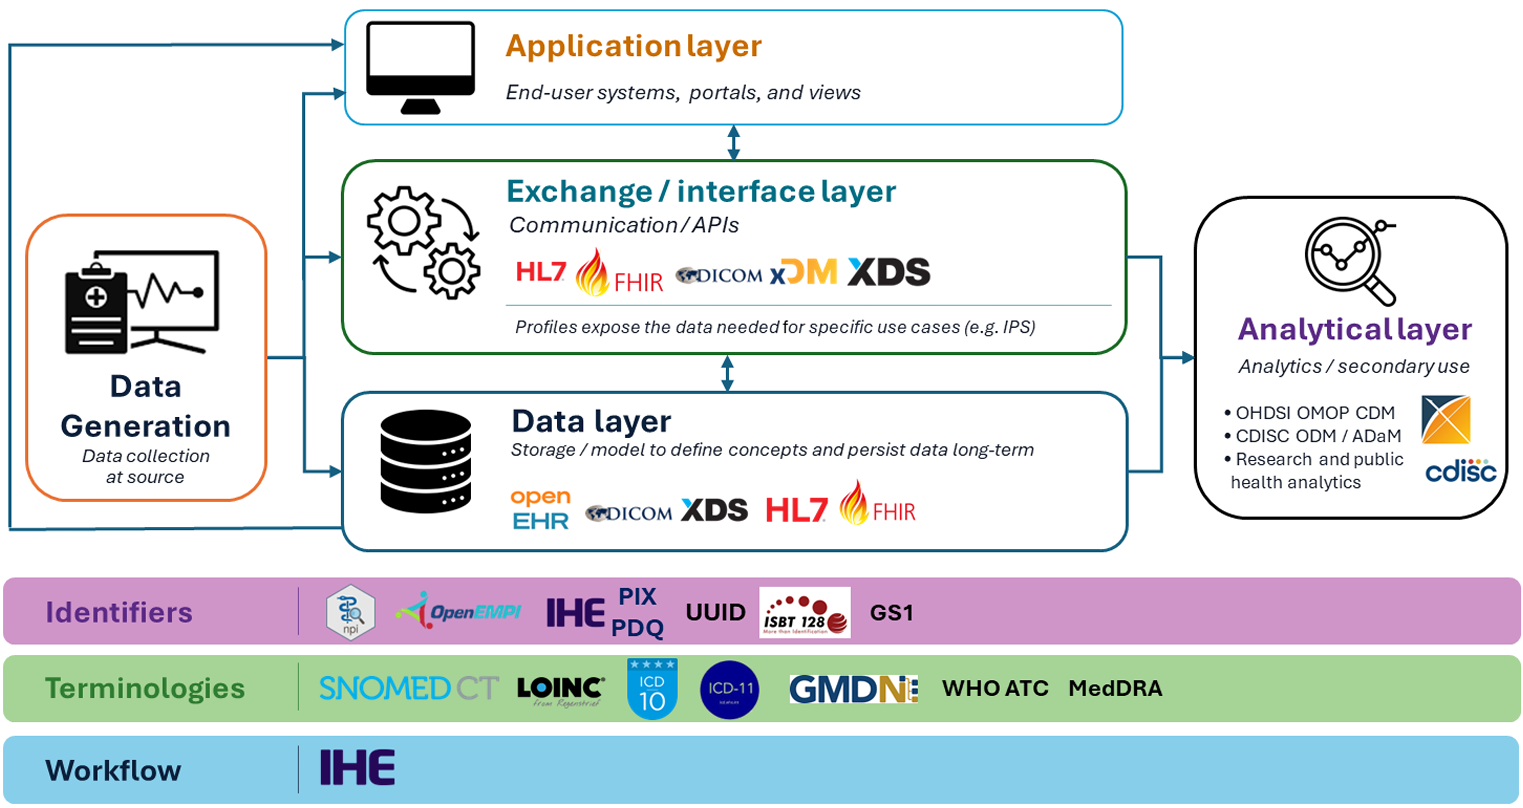
\includegraphics[width=\textwidth]{figures/fig2.png}
    \caption{Examples of available health data standards and their roles in interoperability. The figure is reproduced from~\cite{oecd_interoperability_2026}; the standards shown are illustrative and not prescriptive for all use cases.}
    \label{fig:health_data_standards}
\end{figure}

\paragraph{The European Health Data Space.}

Regulatory frameworks and legislation are fundamental to successful interoperability efforts~\cite{oecd_interoperability_2026}. Beyond technical standards, effective health data sharing requires common rules governing access, exchange, and reuse. In Europe, the European Health Data Space (EHDS) represents a major initiative in this direction, establishing a common framework for the primary and secondary use of electronic health data across Member States~\cite{oecd_interoperability_2026}.

The EHDS brings together technical, organizational, and regulatory elements around a common goal: a patient-centered health data ecosystem in which data are findable, accessible, interoperable, and reusable (FAIR), and can be used effectively and safely in the public interest~\cite{oecd_interoperability_2026}. It aims to facilitate individuals' access to and control over their electronic health data across borders, while supporting their secure reuse for research, innovation, and data-driven policymaking.

By establishing common requirements for data access, interoperability, and reuse, the initiative seeks to address the fragmentation of health data across national and institutional systems~\cite{oecd_interoperability_2026}. This is particularly relevant for AI, which depends on sufficiently large, high-quality, and interoperable datasets for the development, validation, and deployment of models across different healthcare settings~\cite{oecd_progress_2026}.

\paragraph{Transformation pipelines.}
The adoption of data standards requires practical mechanisms for transforming heterogeneous source data into standardized representations. Transformation pipelines operationalize this process through extraction, restructuring, mapping, and validation, supporting interoperability, secondary use, and the preparation of clinical data for analytics and AI~\cite{namli2024scalable,tabari2022state}. Existing approaches have demonstrated the feasibility of transforming heterogeneous clinical data into FHIR-based representations, starting from MIMIC-IV~\cite{bennett2023mimic}, openEHR compositions~\cite{ladas2022openehr}, and OMOP-CDM data~\cite{soares2023omop}. Broader harmonization and metadata-driven integration frameworks have also been proposed~\cite{williams2023standardized,simon2024metadata}. However, these approaches reveal recurring limitations concerning the portability and reusability of mapping processes, which may depend on internal mapping logic, custom scripts, implementation-specific technologies, or manual mapping and validation~\cite{bennett2023mimic,montazeri2023developing,sinaci2023data,williams2023standardized,ladas2022openehr,simon2024metadata}. Declarative and templated mappings can reduce some of these dependencies, although their applicability may remain constrained by specific mapping languages or input models~\cite{sinaci2023data,williams2023standardized,soares2023omop}. More recent work has explored modular FHIR- and RDF-based pipelines for producing research-ready and semantically enriched datasets, while highlighting the need for broader validation and further automation~\cite{carbonaro2025raw}. These limitations motivate transformation mechanisms that provide standardized and shareable mappings while reducing dependence on custom scripts and implementation-specific technologies.

\subsection{Contributions}
\label{subsec:harmonization_contributions}
The contributions associated with the first methodological stage address the transition from heterogeneous data to structured and interoperable information. Within the data-centric perspective adopted by this thesis, this transition is addressed through \emph{Harmonization and Structuring}, where data standards and transformation mechanisms provide the means to establish a common representation across heterogeneous sources. The two contributions investigate complementary aspects of this problem. The first characterizes the current landscape of health data standard adoption and identifies the practical challenges that limit the effective use of standards. The second investigates how standard-based transformation can be operationalized through a modular and reusable pipeline. Although the pipeline was developed before the review was completed, the two are presented together because they address the same transition from two angles: the characterization of the problem and the design of a mechanism for addressing it.

%$\paragraph{Characterizing the adoption of health data standards.}
\paragraph{Paper 1 -- health data standard adoption.}
The first contribution, \emph{Challenges of health data standard adoption and usage: a systematic review}~\cite{marfoglia2026challenges}, investigates how three major health data standards, FHIR, OMOP-CDM, and openEHR, are adopted and used in real-world clinical and research settings. The systematic review analyzes 99 studies published between 2021 and 2024, considering their application domains, use cases, implementation scale, standard coverage, ETL approaches, and the extent to which the standards were adopted as specified or adapted to individual contexts.

The contribution provides an empirical characterization of the conditions under which health data standards are adopted and implemented, with particular attention to the processes through which heterogeneous source data are mapped, transformed, and validated into standardized representations.

From the perspective of the thesis, this contribution constitutes the \emph{problem-characterization} component of the Data--Information transition. It examines the premise that interoperability cannot be reduced to selecting a standard, but also requires appropriate processes for mapping, transforming, validating, and maintaining data across heterogeneous source environments.

%\paragraph{Operationalizing standard-based data transformation.}
\paragraph{Paper 2 -- standard-based data transformation.}
The second contribution, \emph{Towards real-world clinical data standardization: A modular FHIR-driven transformation pipeline to enhance semantic interoperability in healthcare}~\cite{marfoglia_towards_2025}, investigates how the transformation of heterogeneous clinical data into a common standardized representation can be operationalized. The proposed approach combines a templating strategy with the FHIR Mapping Language and separates mapping specifications from their execution. The resulting pipeline adopts a modular architecture organized into five modules: \emph{Input}, \emph{Refinement}, \emph{Mapping}, \emph{Validation}, and \emph{Export}.

The approach was evaluated on a real-world clinical dataset by verifying the transformed resources against data-quality criteria and against queries designed with domain experts.

Within the thesis methodology, this contribution therefore represents the \emph{technical operationalization} of the Data--Information transition. While the systematic review identifies the practical challenges associated with the adoption of health data standards, the transformation pipeline is designed to address part of these challenges, namely implementation-specific and poorly documented mapping processes, through an explicit and modular transformation process intended for reuse. The two contributions consequently connect \emph{understanding the problem} with \emph{engineering a mechanism for addressing it}.

\paragraph{Overall contribution.}
Taken together, these contributions address complementary activities within the \emph{Training Data Development} dimension of data-centric AI~\cite{zha_data-centric_2025}. The systematic review~\cite{marfoglia2026challenges} characterizes the challenges associated with the practical adoption of health data standards, while the FHIR transformation pipeline~\cite{marfoglia_towards_2025} operationalizes \emph{data integration} and \emph{data preparation} through an explicit, modular, and reusable transformation process. The FHIR-standardized data collection resulting from the application of the pipeline has been described in a separate data publication~\cite{arcobelli2024fhir}, which makes the harmonized data available for reuse. Collectively, these contributions illustrate how data-centric principles can be translated into mechanisms for understanding, harmonizing, and preparing heterogeneous data for subsequent computational use.

With respect to FUTURE-AI~\cite{lekadir_future-ai_2025}, this stage is primarily concerned with \emph{Universality}, through the use of existing standards, and with \emph{Traceability}, through the explicit specification and validation of data transformations. The relationship between the contributions and these principles is discussed in Section~\ref{sec:conclusions_trustworthy}.

\section{Semantic Enrichment}
\label{sec:semantic_enrichment}

The second methodological stage addresses the transition from \emph{Information} to \emph{Knowledge}. While harmonization and structuring establish compatible representations for heterogeneous data, standardization alone does not necessarily make their meaning, relationships, and contextual dependencies explicit. This stage therefore extends the data-centric process through semantic technologies that represent domain concepts and relationships in a machine-interpretable form.

It is primarily related to the \emph{Data Maintenance} dimension of data-centric AI, particularly \emph{data understanding} and \emph{data storage and retrieval}~\cite{zha_data-centric_2025}. Within the perspective adopted by this thesis, these activities are extended through formal semantic representations that make domain concepts, relationships, and contextual dependencies explicit and computationally accessible. Semantic Web technologies, ontologies, knowledge graphs, and semantic reasoning provide complementary mechanisms for enriching structured information and establishing a computable knowledge layer. This layer can subsequently support both AI methods and reasoning over interconnected information.

\subsection{Background}
\label{subsec:semantic_background}

\paragraph{Semantic Web.}

The Semantic Web (SW) provides formal mechanisms for representing information and its relationships in a machine-interpretable form~\cite{rathee_semantic_2025}. Among its core technologies, the Resource Description Framework (RDF) provides a graph-based data model for representing information as subject--predicate--object triples, while the Web Ontology Language (OWL) provides a formal language for defining concepts, properties, relationships, and logical constraints~\cite{amato_semfedxai_2025,xhani_role_2025}. Together, these technologies support graph-based representations in which heterogeneous resources can be explicitly connected and queried according to their semantic relationships~\cite{rathee_semantic_2025}.

This capability is particularly relevant to healthcare, where information originates from heterogeneous sources and is expressed using different structures and terminologies. By linking data to external terminologies, ontologies, and controlled vocabularies, Semantic Web technologies associate observations with explicit domain concepts and relationships, supporting data exploration, integration, and validation~\cite{toure2023}. Their extensibility also facilitates the integration of additional resources without requiring the underlying representation to be redesigned~\cite{rathee_semantic_2025}.

From a data-centric perspective, semantic technologies therefore extend data engineering beyond structural consistency by explicitly representing the meaning associated with data. They can also support the implementation of FAIR principles by facilitating semantic interoperability, structured access, knowledge integration, and data validation, although FAIRness ultimately depends on appropriate data governance and stewardship in addition to technological mechanisms~\cite{rathee_semantic_2025}. The role of semantic technologies in this thesis is consequently not limited to enriching datasets with additional metadata, but to establishing representations in which domain meaning can be computationally accessed and exploited.

\paragraph{Ontologies.}

Ontologies provide formal representations of the concepts, properties, and relationships that characterize a domain. By making domain semantics explicit, they establish a shared conceptual basis for interpreting and integrating heterogeneous data~\cite{xhani_role_2025,amato_semfedxai_2025}. In healthcare, resources such as SNOMED CT, LOINC, and ICD-10 illustrate the role of formalized vocabularies in representing clinical and biomedical concepts~\cite{amato_semfedxai_2025}.

By associating data elements with explicit domain concepts and relationships, ontologies support \emph{data understanding} and can reduce ambiguity arising from heterogeneous representations. They can also provide a semantic interface between data and AI methods by linking model features, predictions, or explanations to domain concepts. For example, medical ontologies have been used to enrich XAI outputs with clinically relevant contextual knowledge~\cite{corbucci_semantic_2023}, while DoctorXAI links features from sequential clinical data to ontology concepts to generate semantically meaningful explanations~\cite{panigutti_role_2023}.

In this sense, ontologies can complement XAI methods by providing the domain concepts and relationships through which AI outputs can be interpreted, although semantic representations alone do not guarantee explainability~\cite{xhani_role_2025}. Rather, they provide a structured semantic basis upon which explanation mechanisms can be constructed and contextualized.

\paragraph{Knowledge Graphs.}

Knowledge Graphs (KGs) represent interconnected entities and relationships in a graph-based structure. In Semantic Web applications, they are commonly represented using RDF and can be associated with ontologies that provide the conceptual semantics of the represented entities and relations~\cite{xhani_role_2025}. In this setting, ontologies provide the conceptual semantics used to describe a domain, while knowledge graphs instantiate such semantics through concrete entities, facts, and relationships.

This combination facilitates the integration of heterogeneous information while supporting semantic querying, provenance representation, and reasoning over interconnected data~\cite{xhani_role_2025}. It is particularly relevant to healthcare, where clinically meaningful information involves relationships among patients, observations, diagnoses, medications, procedures, and temporal events. Healthcare KGs have consequently been investigated for applications including diagnosis, drug-interaction detection, and personalized treatment~\cite{amato_semfedxai_2025}.

The resulting graph structure can also be exploited directly by AI methods. Graph-based learning approaches operate on entities and relations, while neuro-symbolic approaches combine learned representations with structured knowledge and formal reasoning~\cite{garcez_neurosymbolic_2023,yang_give_2024}. KGs therefore provide not only an alternative representation of data, but also a structured substrate through which semantic knowledge can be integrated with computational models.

Knowledge graphs have accordingly been investigated as a means of building knowledge-enriched AI systems. Because the represented information retains its semantics and remains machine-interpretable, AI methods operating on knowledge graphs can exploit contextual relationships in addition to statistical patterns in the data~\cite{maree_quantifying_2025}. Whether and how the design of such representations affects model performance is, however, rarely examined explicitly; this question is addressed by the third contribution of the thesis.


\paragraph{Semantic Inference and Reasoning.}

Explicit semantic representations can further support the derivation of knowledge that is not directly encoded in the original data. Ontologies provide the conceptual structures and logical constraints for representing domain knowledge, while rule-based formalisms such as the Semantic Web Rule Language (SWRL) enable additional facts to be inferred from explicitly represented information.

This capability has been explored to combine machine learning with explicit domain reasoning in healthcare-oriented AI systems~\cite{sharma_ontoxai_2024}. More broadly, neuro-symbolic approaches combine the representation and reasoning capabilities of symbolic systems with the predictive capabilities of neural networks~\cite{garcez_neurosymbolic_2023,bhuyan_neuro-symbolic_2024,yang_give_2024}. Recent approaches have also investigated the transformation of learned neural behavior into symbolic rules or knowledge representations, making aspects of model behavior more explicit and amenable to reasoning~\cite{terziyan_semantic_2026}. For example, OntoXAI uses SWRL-based representations to generate explanations from classification rules~\cite{sharma_ontoxai_2024}, while other neural-symbolic approaches integrate deep learning with ontologies and knowledge graphs to align learned representations with structured knowledge and support reasoning across heterogeneous information sources~\cite{cheng_neural-symbolic_2024}.

Overall, semantic representations provide the formal basis for making domain knowledge explicit and computationally accessible. The resulting knowledge can then be queried, integrated, and subjected to logical or computational inference. Within the data-centric perspective of this thesis, these mechanisms therefore provide the means through which structured information can be transformed into a machine-interpretable knowledge layer. Their subsequent exploitation for prediction, simulation, and decision support is considered in the \emph{Inference and Reasoning} stage.

\subsection{Contributions}
\label{subsec:semantic_contributions}

The contributions associated with the second methodological stage address the transition from structured \emph{Information} to machine-interpretable \emph{Knowledge}. Building on standardized representations of the kind established in the previous stage, they investigate how semantic models can make both clinical data and computational resources explicitly representable and exploitable by AI systems. The two contributions address complementary aspects of this problem: the first focuses on the semantic representation of clinical event data and its integration with graph-based learning, while the second extends semantic representation to machine-learning models for personalized healthcare.

\paragraph{Paper 3 -- semantic representation of clinical data.}

The third contribution, \emph{MEDS-OWL: An Ontology-Driven Framework for Clinical Outcome Prediction with Graph Learning}~\cite{marfoglia_meds-owl_2026}, investigates how an event-centric representation of longitudinal clinical data can be transformed into a semantically explicit knowledge representation suitable for both data integration and graph-based learning. The work builds on the Medical Event Data Standard (MEDS), which provides a unified event-centric representation designed to support reproducible machine-learning workflows, but does not natively provide an ontology-level semantic representation. The contribution addresses this gap through \emph{MEDS-OWL}, a lightweight OWL ontology for MEDS, and \emph{meds2rdf}, a scalable framework for transforming MEDS-compliant datasets into RDF-based knowledge graphs.

The resulting representation preserves the event-centric structure of MEDS while introducing explicit semantics and relationships among subjects, events, and clinical concepts. The framework also enables links to external biomedical vocabularies, providing a basis for semantic integration and further enrichment of the generated knowledge graphs. The work therefore extends a standardized machine-learning-oriented data representation with an explicit semantic layer without requiring changes to the underlying MEDS model.

The contribution further investigates the role of semantic representation in AI by systematically varying the granularity of the relationships encoded in the resulting knowledge graphs. The framework was evaluated for conversion fidelity and scalability on four heterogeneous clinical datasets, comprising more than 309,000 hospital stays, and the effect of granularity was assessed on 11 clinical outcome prediction tasks using a Relational Graph Convolutional Network and tabular baselines.

Within the thesis methodology, this contribution therefore represents the \emph{semantic operationalization} of the Information--Knowledge transition. Starting from a standardized representation, in this case MEDS and not the FHIR output of the previous stage, it introduces explicit meaning and relationships, and examines whether these representational choices influence how the resulting knowledge can be exploited by AI methods.

\paragraph{Paper 4 -- semantic representation of ML models.}

The fourth contribution, \emph{Representation of ML Models to Enhance Simulation Capabilities Within Digital Twins in Personalized Healthcare}~\cite{marfoglia_2024_mimo}, extends semantic representation beyond clinical data to the computational capabilities that operate on them. The work builds on the CONNECTED framework, which integrates heterogeneous healthcare data, FHIR-compliant representations, Personal Knowledge Graphs, and Digital Twins to support patient-specific services and predictive simulation.

The contribution introduces the \emph{Manifest} concept: a formal, machine-readable description of executable ML models, based on an OWL ontology, that specifies their inputs, outputs, metadata, and location. These descriptions are represented in RDF and linked to the semantic resources of the Digital Twin, so that a reasoner can relate model input requirements to the available FHIR-based patient data and invoke a model when its required inputs are satisfied. Paper~4 presents this design conceptually and illustrates it with a cardiovascular-risk example; its implementation and evaluation, through the Model Interface Manifest Ontology (MIMO), are reported in Paper~6. Paper~4 also extends the CONNECTED architecture introduced in Paper~5, but is presented in this stage because its contribution is the formal representation of model interfaces rather than their operational integration.

Within the thesis methodology, this contribution extends the Information--Knowledge transition from the representation of clinical information to the representation of \emph{computational capabilities}. While MEDS-OWL makes clinical entities and their relationships explicit, the Manifest makes the interfaces and metadata of AI models explicit, allowing data and computational resources to be connected within a common semantic environment. This representation makes computational capabilities identifiable and machine-interpretable, providing a semantic basis for their automated discovery, integration, and orchestration within an AI-enabled Digital Twin.

\paragraph{Overall contribution.}

Taken together, these contributions extend the data-centric perspective from the preparation of structured information to its maintenance, interpretation, and accessibility through explicit semantic representations. They operationalize aspects of the \emph{Data Maintenance} dimension by addressing complementary activities related to \emph{data understanding} and \emph{data storage and retrieval}~\cite{zha_data-centric_2025}. Data understanding is addressed through the formalization of the meaning and relationships of clinical information, while storage and retrieval are extended through semantic representations that make clinical data and computational resources identifiable, queryable, and reusable.

From the perspective of the thesis, \emph{Semantic Enrichment} therefore operationalizes Data Maintenance by transforming structured information into a semantically organized and reusable knowledge space. The resulting computable knowledge layer provides a common environment in which clinical entities, relationships, and computational capabilities can be explicitly represented and connected. This establishes the basis for the subsequent \emph{Inference and Reasoning} stage, where the resulting knowledge and computational capabilities can be exploited for prediction, simulation, and decision support.

With respect to FUTURE-AI~\cite{lekadir_future-ai_2025}, this stage is primarily concerned with \emph{Universality} and \emph{Traceability}, through the explicit, standard-based representation of clinical data and model interfaces, and was designed to provide context on which \emph{Explainability} mechanisms could build. The relationship between the contributions and these principles is discussed in Section~\ref{sec:conclusions_trustworthy}.

\section{Inference and Reasoning}
\label{sec:inference_reasoning}

The third methodological stage addresses the transition from \emph{Knowledge} to actionable insights that can support informed and human-centered decision-making. While semantic enrichment establishes explicit and machine-interpretable representations of domain knowledge, this stage concerns the exploitation of such knowledge through inference, prediction, simulation, and AI-supported analysis. The objective is therefore not simply to represent information more richly, but to create an environment in which data, semantic knowledge, and computational capabilities can be combined to derive and evaluate context-dependent insights.

Within the data-centric perspective adopted by this thesis, this stage extends \emph{Data Maintenance}~\cite{zha_data-centric_2025} from the preparation and representation of data towards their use by AI models in dynamic computational environments. In operational AI systems, data sources, patient states, computational environments, and intended uses may evolve over time. This makes \emph{data quality assurance}, the continuous assessment of the information provided to AI methods and of the conditions under which their outputs are generated, an important requirement of this stage~\cite{zha_data-centric_2025}. The contributions of this thesis establish the integration environment in which such assessment could take place, but do not themselves implement or evaluate continuous data quality assurance. Digital Twins provide an architectural environment for integrating data, knowledge, and computational models, while explainability and human-in-the-loop mechanisms support the interpretation, assessment, and appropriate use of the resulting outputs.

\subsection{Background}
\label{subsec:inference_background}

\paragraph{Digital Twins.}

Digital Twins (DTs) have traditionally been used to represent, monitor, and simulate physical entities and processes across different application domains. In healthcare, they have emerged as an enabling technology for Healthcare 4.0, supporting applications such as patient monitoring, personalized treatment planning, clinical process optimization, and simulation~\cite{9255249_erol,9900390_alazab,Björnsson2019,Katsoulakis2024}. Their applications span different levels of abstraction, including human- and organ-level modeling, treatment and drug-interaction simulation, remote healthcare, hospital resource management, medical-device monitoring, and the representation of healthcare processes and workflows~\cite{SHENGLI2021100014,Björnsson2019,9325551_ricci,8846667_yang_peng,9320532_elayan_haya}. In particular, Human Digital Twins aim to integrate heterogeneous biological, genetic, lifestyle, and clinical information to support the evaluation of possible interventions and future health states in a virtual environment~\cite{SHENGLI2021100014,Björnsson2019}.

The increasing availability of heterogeneous and continuously generated data has progressively expanded the role of DTs beyond static representation and simulation. More recent approaches conceptualize DTs as information-rich computational environments in which heterogeneous data, semantic representations, and computational models are integrated to support monitoring, analysis, prediction, and simulation~\cite{felicetti_knowledge_2025,Katsoulakis2024}. Within such architectures, ontologies can provide a semantic foundation for representing domain concepts and relationships, while knowledge graphs support the integration of heterogeneous entities and contextual information~\cite{boje_towards_2020,albers_semantic_2020}. AI methods can then operate on this structured environment to identify patterns, generate predictions, and support simulation and decision-making~\cite{felicetti_knowledge_2025}. This evolution changes the role of the Digital Twin within the overall data-centric process. Rather than representing a physical or clinical entity in isolation, the DT can act as an integration layer connecting the different elements required for computational analysis.

Such an environment is particularly relevant to personalized healthcare, where patient-specific information can be combined with predictive models and simulation mechanisms to investigate possible trajectories or interventions~\cite{Katsoulakis2024}. At the same time, the increasing complexity of these environments introduces additional requirements concerning data quality, semantic consistency, privacy and security, and the validation and appropriate use of computational models~\cite{Katsoulakis2024}. Consequently, the reliability of a healthcare DT depends not only on the predictive capabilities of its constituent models, but also on the quality and contextual validity of the data, knowledge, and computational relationships supporting them.

\paragraph{Human-in-the-Loop and XAI.}

The exploitation of AI-generated knowledge in healthcare also requires mechanisms through which computational outputs can be interpreted, assessed, and appropriately incorporated into human decision-making. Human-in-the-loop approaches therefore maintain human involvement in relevant stages of the AI workflow, including the interpretation of outputs, validation of system behavior, and assessment of AI-supported decisions~\cite{kaur_trustworthy_2022,felicetti_knowledge_2025}. Human involvement is particularly important in healthcare because computational outputs are ultimately interpreted within clinical and organizational contexts that cannot be reduced to the information available to an individual model.

Explainable AI (XAI) provides a complementary set of mechanisms for supporting this interaction by making aspects of model behavior or individual predictions more understandable to human stakeholders~\cite{guidotti_survey_2019,miller_explanation_2019}. Depending on the application and intended user, explanations may concern individual predictions or provide more general information about model behavior~\cite{murdoch_interpretable_2019,xhani_role_2025,kaur_trustworthy_2022}. They can support activities such as model inspection, debugging, identification of potentially problematic behavior, and feature analysis~\cite{10.1145/2939672.2939778_ribeiro}. However, the adequacy of an explanation depends on its intended purpose, scope, and audience, particularly in healthcare where explanations must be meaningful within the relevant clinical context~\cite{kaur_trustworthy_2022}.

The need for such mechanisms becomes more pronounced as Digital Twins evolve towards adaptive systems that combine heterogeneous data, semantic knowledge, and AI models for prediction and simulation~\cite{felicetti_knowledge_2025}. Machine-learning models can identify complex statistical patterns, but their outputs do not necessarily expose the domain knowledge or contextual relationships underlying those patterns~\cite{felicetti_knowledge_2025}. Semantic technologies can complement this capability by providing an explicit contextual layer through which data, concepts, relationships, and computational resources can be connected~\cite{boje_towards_2020,albers_semantic_2020}. Ontologies and knowledge graphs can consequently support the interpretation of model inputs and outputs by relating them to domain concepts and contextual information~\cite{xhani_role_2025}, while expert-curated semantic structures can provide additional constraints for reducing unsupported interpretations or inferences~\cite{karabulut_ontologies_2024}.

Within this perspective, semantic representation and explainability address complementary aspects of human understanding. XAI provides mechanisms for exposing relevant aspects of model behavior, whereas semantic representations provide the domain context through which computational outputs can be related to concepts, entities, and relationships~\cite{xhani_role_2025,corbucci_semantic_2023,panigutti_role_2023}. Their combination can therefore support a workflow in which human stakeholders receive computationally derived insights, relate them to the underlying patient and domain context, and assess their relevance before incorporating them into decision-making~\cite{felicetti_knowledge_2025}. Importantly, neither semantic representation nor explanation alone guarantees correctness, reliability, or appropriate use. Rather, they provide technical mechanisms that can support human understanding and oversight within a broader Trustworthy AI lifecycle.

\subsection{Contributions}
\label{subsec:inference_contributions}

The contributions associated with the third methodological stage investigate how semantically represented \emph{Knowledge} can be exploited for AI-supported analysis, corresponding to the \emph{Wisdom} level as interpreted in this thesis. They focus on computational environments in which patient information can be used by AI models to predict possible health states and support personalized care.

The two contributions follow a progressive trajectory. The first introduces the architectural foundations for integrating heterogeneous and standardized patient data within a Digital Twin~\cite{10.3389/fdgth.2023.1322428_carbonaro_connected}. The second implements this architecture and extends it with predictive capabilities provided by AI models~\cite{MARFOGLIA2026108380}, exposed through a standard interface that hides the underlying integration complexity. The resulting environment returns model outputs within the context of the patient's Digital Twin.

\paragraph{Paper 5 -- Digital Twins and Personal Knowledge Graphs.}
The fifth contribution, \emph{CONNECTED: leveraging digital twins and personal knowledge graphs in healthcare digitalization}~\cite{10.3389/fdgth.2023.1322428_carbonaro_connected}, investigates how Digital Twins and knowledge graphs can provide an architectural foundation for integrating heterogeneous healthcare data and supporting intelligent applications. The gathered and harmonized data are used to populate patient-specific Digital Twins. The resulting virtual replicas provide a persistent representation of patient information and establish the basis for analytical and simulation capabilities.

The framework is defined through four layers (\emph{Source}, \emph{Standard}, \emph{Digital Twin}, and \emph{Application}) derived from requirements identified in the literature, and its expressiveness is illustrated through a fall-risk scenario. From a data-centric perspective, the contribution recognizes that patient-specific representations depend on the availability and evolution of their underlying data sources, so that the information supporting downstream computation must remain structured, coherent, and up to date. The Digital Twin provides an environment in which patient data can be maintained within their computational context, and the paper identifies data integrity and validity as open challenges for such environments.

\paragraph{Paper 6 -- AI-powered patient Digital Twins.}
The sixth contribution, \emph{A knowledge graph-driven framework for deploying AI-powered patient digital twins}~\cite{MARFOGLIA2026108380}, extends CONNECTED towards the integration and operational use of AI models within the Digital Twin. It enables the virtual replica to dynamically connect patient-specific information with computational models and support predictive simulation.

A key contribution is the automation of model integration. Through the Manifest protocol and MIMO, a reasoner binds the input requirements of each model to the patient data held in the Digital Twin, and the model is invoked through a FHIR-compliant API only when all required inputs are available. The mechanism was evaluated on a stroke-risk use case through three analyses: the functional equivalence of Manifest-driven and standalone model execution, a proof-of-concept application benchmarking several classifiers integrated through the same interface, and a performance evaluation of the platform's latency and throughput.

\paragraph{Overall contribution.}
Taken together, these contributions address the transition from \emph{Knowledge} to actionable insights. They combine semantically enriched patient information with AI models and simulation capabilities. CONNECTED provides the architectural foundation for integrating heterogeneous and standardized patient data within a Digital Twin backed by a knowledge graph. The subsequent framework extends this foundation towards the operational integration of AI models and predictive simulation.

From a data-centric perspective, this stage extends \emph{Data Maintenance} into the operational use of data by AI models~\cite{zha_data-centric_2025}. Patient data, semantic representations, and AI models are maintained within a common computational environment, so that the data used by a model and the conditions under which it is invoked are explicitly represented. This provides a basis on which continuous data quality assurance could be built, although such assurance is not implemented in the current contributions. The Digital Twin therefore acts as an integration layer between the \emph{Knowledge} established in the previous stage and its computational exploitation.

With respect to FUTURE-AI~\cite{lekadir_future-ai_2025}, this stage is primarily concerned with \emph{Traceability}, through the explicit binding between patient data and model inputs, and was designed with \emph{Usability} and \emph{Explainability} in mind, with the aim of supporting rather than replacing human judgment. The relationship between the contributions and these principles is discussed in Section~\ref{sec:conclusions_trustworthy}.


\chapter{Harmonization and Structuring}
\label{chap:harmonization_structuring}
This chapter contains the two contributions associated with the \emph{Harmonization and Structuring} stage described in Section~\ref{sec:harmonization_structuring}: Paper~1 (Section~\ref{sec:paper1}) and Paper~2 (Section~\ref{sec:paper2}). Together, they address RQ1, which is answered in Section~\ref{subsec:conclusions_rq1}.

% ============================================================================
% Paper 1 -- converted to LaTeX from the published article (J. Biomed. Inform. 178 (2026) 105022, PDF supplied in
% papers/1-s2.0-S1532046426000468-main.pdf). No Word version of the paper was supplied. Generated by a conversion
% script from the PDF text layer; see the integration report for the conversion procedure and known issues.
% ============================================================================
\section{Challenges of health data standard adoption and usage: a systematic review}
\label{sec:paper1}

\noindent This section contains the article~\cite{marfoglia2026challenges}.

\paragraph{Authors.}
Alberto Marfoglia\textsuperscript{a}, Valerio Antonio Arcobelli\textsuperscript{b,*}, Serena Moscato\textsuperscript{b}, Antonino Amedeo La Mattina\textsuperscript{c}, Sabato Mellone\textsuperscript{b}, Antonella Carbonaro\textsuperscript{a}

{\raggedright % layout: ragged-right metadata block
\noindent\textsuperscript{a}Department of Computer Science and Engineering - DISI, University of Bologna, Via dell'Universit\`a 50, 47521 Cesena, Italy\\
\textsuperscript{b}Department of Electrical, Electronic and Information Engineering ``Guglielmo Marconi'' -- DEI, University of Bologna, Viale del Risorgimento 2, 40136 Bologna, Italy\\
\textsuperscript{c}Medical Technology Lab, IRCCS Istituto Ortopedico Rizzoli, Bologna, Italy\\
\textsuperscript{*}Corresponding author. E-mail address: valerio.arcobelli2@unibo.it (V.A. Arcobelli).\\
Journal of Biomedical Informatics 178 (2026) 105022. \url{https://doi.org/10.1016/j.jbi.2026.105022}. Received 28 August 2025; Received in revised form 29 January 2026; Accepted 17 March 2026; Available online 21 March 2026. 1532-0464/\textcopyright{} 2026 The Author(s). Published by Elsevier Inc. This is an open access article under the CC BY license (\url{http://creativecommons.org/licenses/by/4.0/}).
\par}

\subsection*{Abstract}

Objective: To explore the adoption and practical implementation of the three major health data standards (i.e., FHIR, OMOP-CDM, and openEHR), to evaluate their maturity level in terms of how extensively they have been applied and integrated into everyday clinical and research practice.\\
Methods: We conducted a systematic review registered in PROSPERO (CRD42024623398) following PRISMA guidelines. Literature searches were performed through PubMed, Cochrane, Scopus, Web of Science, and IEEE Xplore from 2021 to 2024. After de-duplication and screening, 99 studies were included. Data was extracted and classified according to five health application domains and five use cases based on the intended purpose of the standard in the work. Studies were assessed for implementation scale, ETL tools, coverage of the standard (i.e., the number of mapped source variables), and whether standards were adapted or used as-is.\\
Results: Of the 99 included studies, 57\% used OMOP-CDM, 39\% FHIR, and 8\% openEHR. Most applications occurred in research settings (87\%) and focused on data reuse (47\%) or clinical decision support (23\%). OMOP-CDM was preferred for large-scale, longitudinal research, while FHIR was dominant in the public health domain and for real-time data exchange. Only 27\% of studies reported the coverage of the standard. FHIR implementations often require customization, complicating interoperability. OMOP-CDM offered strong analytical tooling but posed challenges for mapping and data loss. Few studies using openEHR reported limitations, with its uptake remaining limited.\\
Conclusion: Although FHIR, OMOP-CDM, and openEHR hold significant potential to enhance interoperability, their adoption remains fragmented. Each standard shows specific strengths: FHIR for exchange, OMOP-CDM for analytics, and openEHR for data persistence. A hybrid approach and clearer implementation practices are essential to support scalable, interoperable health data ecosystems.

\paragraph{Keywords:} Health data standard; Interoperability; Health informatics

\begin{table}[htbp]
\centering
\begin{tabular}{p{0.28\textwidth} p{0.62\textwidth}}
\hline
\textbf{Problem or Issue} &
Despite growing availability of health data standards, their real-world adoption remains fragmented, and the maturity and integration of the major health data standards (i.e., FHIR, OMOP-CDM, and openEHR) are not well characterized.
\\[0.5em]
\textbf{What is Already Known} &
FHIR, OMOP-CDM, and openEHR each support specific aspects of health data interoperability. Existing literature focuses mostly on isolated implementations or theoretical comparisons, without mapping actual usage.
\\[0.5em]
\textbf{What this Paper Adds} &
This paper systematically reviews 99 studies to assess how, where, and why these standards are used in real-world settings. It identifies gaps in ETL reporting, extension practices, and proposes a hybrid ecosystem model.
\\[0.5em]
\textbf{Who would benefit from the new knowledge in this paper} &
Health informatics researchers, standard developers, policymakers, and system integrators seeking to improve interoperability and guide informed standard adoption across healthcare and research domains.
\\
\hline
\end{tabular}
\end{table}

\subsection{Introduction}
\label{sec:paper1_introduction}

The healthcare industry generates about 30\% of the world's data volume \cite{thomason_data_2024} from various sources \cite{leavy_data_2019}, including electronic health records (EHRs) \cite{wang_electronic_2023}, administrative information \cite{cadarette_introduction_2015}, laboratory systems \cite{harrison_role_2008}, imaging systems \cite{noauthor_medical_2018}, medical devices \cite{moscato_wrist_2022,arcobelli_enhancing_2024,arcobelli_mcrutch_2023}, and consumer devices \cite{piwek_rise_2016}. In this scenario, data standardization has garnered significant attention in recent years as a pivotal step to efficiently exploit this precious source of information. The widespread adoption of standards in various applications, such as clinical trials, hospital information systems, and public health data streams, provides significant enhancements in communication and optimization of patient care workflows \cite{pimenta_interoperability_2023}. By leveraging seamless exchange and sharing of data, standardization enables continuity of care across all levels of the health system, independently of the specific software in use \cite{torab-miandoab_interoperability_2023}. Moreover, the adoption of a standardized framework for healthcare data interoperability offers significant benefits for the secondary use of real-world data in medical data science, including cost efficiency, improved data quality, and exceptional analytical flexibility \cite{gehrmann_what_2023}.

Despite the promising aspects of the health data standard adoption in clinical settings, there are still some concerns about its widespread use. The main challenges are political and technical. The former category, being among the most difficult obstacles to overcome \cite{shankardass_implementation_2018}), primarily arises due to an extreme heterogeneity in local policy adoption, often lacking a ``Health in All Policies'' approach \cite{noauthor_health_2006} fostering cross-sector collaboration to achieve common goals in the health domain; policy fragmentation is exacerbated by the frequent policy changes implemented to address public health issues. On the other hand, technical challenges result from the heterogeneous landscape of architectures, formats, applications, tools, and vendors that have independently contributed to the development of information systems across hospitals, healthcare organizations, and research institutions. In this context, concerns persist regarding the large-scale adoption of Extract, Transform, Load (ETL) processes due to the lack of common best practices \cite{pollack_porter_importance_2018}. Although some efforts have been made in proposing approaches to mitigate technical heterogeneity \cite{marfoglia_towards_2025,arcobelli_motu_2023,bennett2023mimic,williams2023standardized}, challenges remain in achieving interoperability and efficiency across diverse systems and platforms.

Such challenges have also been raised in the development of the European Health Data Space (EHDS) initiative, aiming to create a unified health data ecosystem to improve data access in healthcare and facilitate secondary use for research and innovation in Europe \cite{noauthor_european_2025}. The preparatory, development, and discussion phases of the EHDS regulation clearly revealed significant fragmentation in the adoption of standard formats and vocabularies, as well as a lack of best practices and reference technical requirements.

Efforts in health data standardization have led to the development of several standards, such as Fast Healthcare Interoperability Resources (FHIR), maintained by Health Level 7 (HL7) \cite{noauthor_index_fhir} and representing healthcare concepts through structured resources and standardized vocabularies such as SNOMED CT and ICD \cite{arcobelli2024fhir}, Observational Medical Outcomes Partnership Common Data Model (OMOP-CDM), maintained by Observational Health Data Sciences and Informatics (OHDSI) \cite{reinecke_usage_2021}, being a rapidly growing open-science research community that enables researchers worldwide to conduct network studies using standardized data and vocabularies \cite{reinecke_usage_2021}, and openEHR, maintained by the openEHR Foundation \cite{kalra_openehr_2005}.

While various studies have explored the application of health data standards in specific contexts, there is no consensus on a universally superior standard. For example, several clinical decision support systems have been independently developed using OMOP-CDM \cite{sadsad_computable_2023}, openEHR \cite{li_configurable_2022}, or FHIR \cite{ulgu_nationwide_2024}, while data exchange services have been implemented using either FHIR \cite{noauthor_fhir_gics_pubmed} or OMOP-CDM \cite{almeida_methodology_2021}. This lack of clarity also extends to real-world applications, beyond controlled research environments where standards are often tested on synthetic or limited datasets.

In this systematic review, we aim to clarify the real-world applications, challenges, and benefits of the adoption of health data standards to inform future research and practice, ultimately identifying which standards are the most suitable for different applications. To achieve this, our primary research question is: ``What is the maturity level of health data standard adoption in real-world settings?''. In this paper, the term maturity is used as a qualitative concept, referring to standards' practical use, integration, and impact in real-world contexts, rather than a quantitative evaluative measure of the standard's progress. We aim to identify evidence of the practical use, integration, and impact of health data standards in real-world contexts.

Given the complexity of this field, we have further divided our primary research question into the following secondary review questions:

\begin{itemize}
  \item[i)] What are the main characteristics and applications of standardized health data?
  \item[ii)] How is health data standardization achieved?
  \item[iii)] How extensive is the use of standardized data in relation to the total data utilized for application implementation?
  \item[iv)] What are the main limitations and barriers to the application of health data standards?
\end{itemize}

\subsection{Related works}
\label{sec:paper1_related_works}

Previous systematic reviews have examined the implementation and adoption of individual standards like FHIR or openEHR, but few have addressed them together with OMOP-CDM in real-world settings. For example, some comprehensive systematic reviews focused exclusively on FHIR implementations in health research settings highlighted its growing use for interoperability and app development \cite{vorisek_fast_2022,kapitan_data_2025,ayaz_fast_2021} while some others focused only on the application of OMOP-CDM \cite{ahmadi_omop_2022,henke_conceptual_2024}. Other works have explored frameworks for aligning multiple standards: a German initiative mapped microbiology data across openEHR, FHIR, and OMOP-CDM, demonstrating-- how cross-standard integration can enhance both exchange and analytic capabilities \cite{rinaldi_from_2021}. More recently, the emerging ``OMOP--onFHIR'' paradigm, using FHIR Bundles for --real-time clinical data exchange with downstream conversion into OMOP--CDM to support global research and semantics preservation, has gained tractio--n \cite{jayathissa_omop-on-fhir_2025}. Thus, given the scenario in which the development of health data standards is rapidly increasing, this underscores both the promise and complexity of integrating FHIR, OMOP-CDM, and openEHR, while also reinforcing the need for this comprehensive systematic mapping of maturity, use cases, and integration pathways in real-world settings among these three widely adopted health data standards.

\subsection{Methods}
\label{sec:paper1_methods}

\subsubsection{Search strategy}
\label{sec:paper1_search_strategy}

The review and research protocol were registered in PROSPERO (CRD42024623398). We adopted the Preferred Reporting Items for Systematic reviews and Meta-Analyses (PRISMA) statement \cite{page_prisma_2021} to ensure high transparency and reproducibility of the review process.

A comprehensive literature search was conducted across the following databases: Cochrane, Scopus, PubMed, IEEE Xplore, and Web of Science. The search strategy was informed by the expertise and experience of the authors and focused on three primary concepts: (1) health data standards, (2) design for application in clinical and research settings, and (3) interoperability. The search query, developed in alignment with these concepts, included relevant terms and synonyms. The adopted query is reported in Text 1 of the Supplementary Material.

\subsubsection{Study selection}
\label{sec:paper1_study_selection}

Duplicates were systematically removed via Systematic Review Accelerator \cite{clark_full_2020,forbes_automation_2024}, and all the retrieved records were then managed using the Rayyan platform \cite{ouzzani_rayyan_2016}. The initial pool of papers was screened based on the inclusion and exclusion criteria by a team of five reviewers (AM, VAA, SeM, AALM, AC), with at least two reviewers independently evaluating each paper to ensure consistency and reliability. Titles and abstracts were examined first, followed by full-text reviews of the selected articles. Any discrepancies between the reviewers were resolved through discussion or by consulting a third reviewer.

\begin{figure}[tbp]
\centering
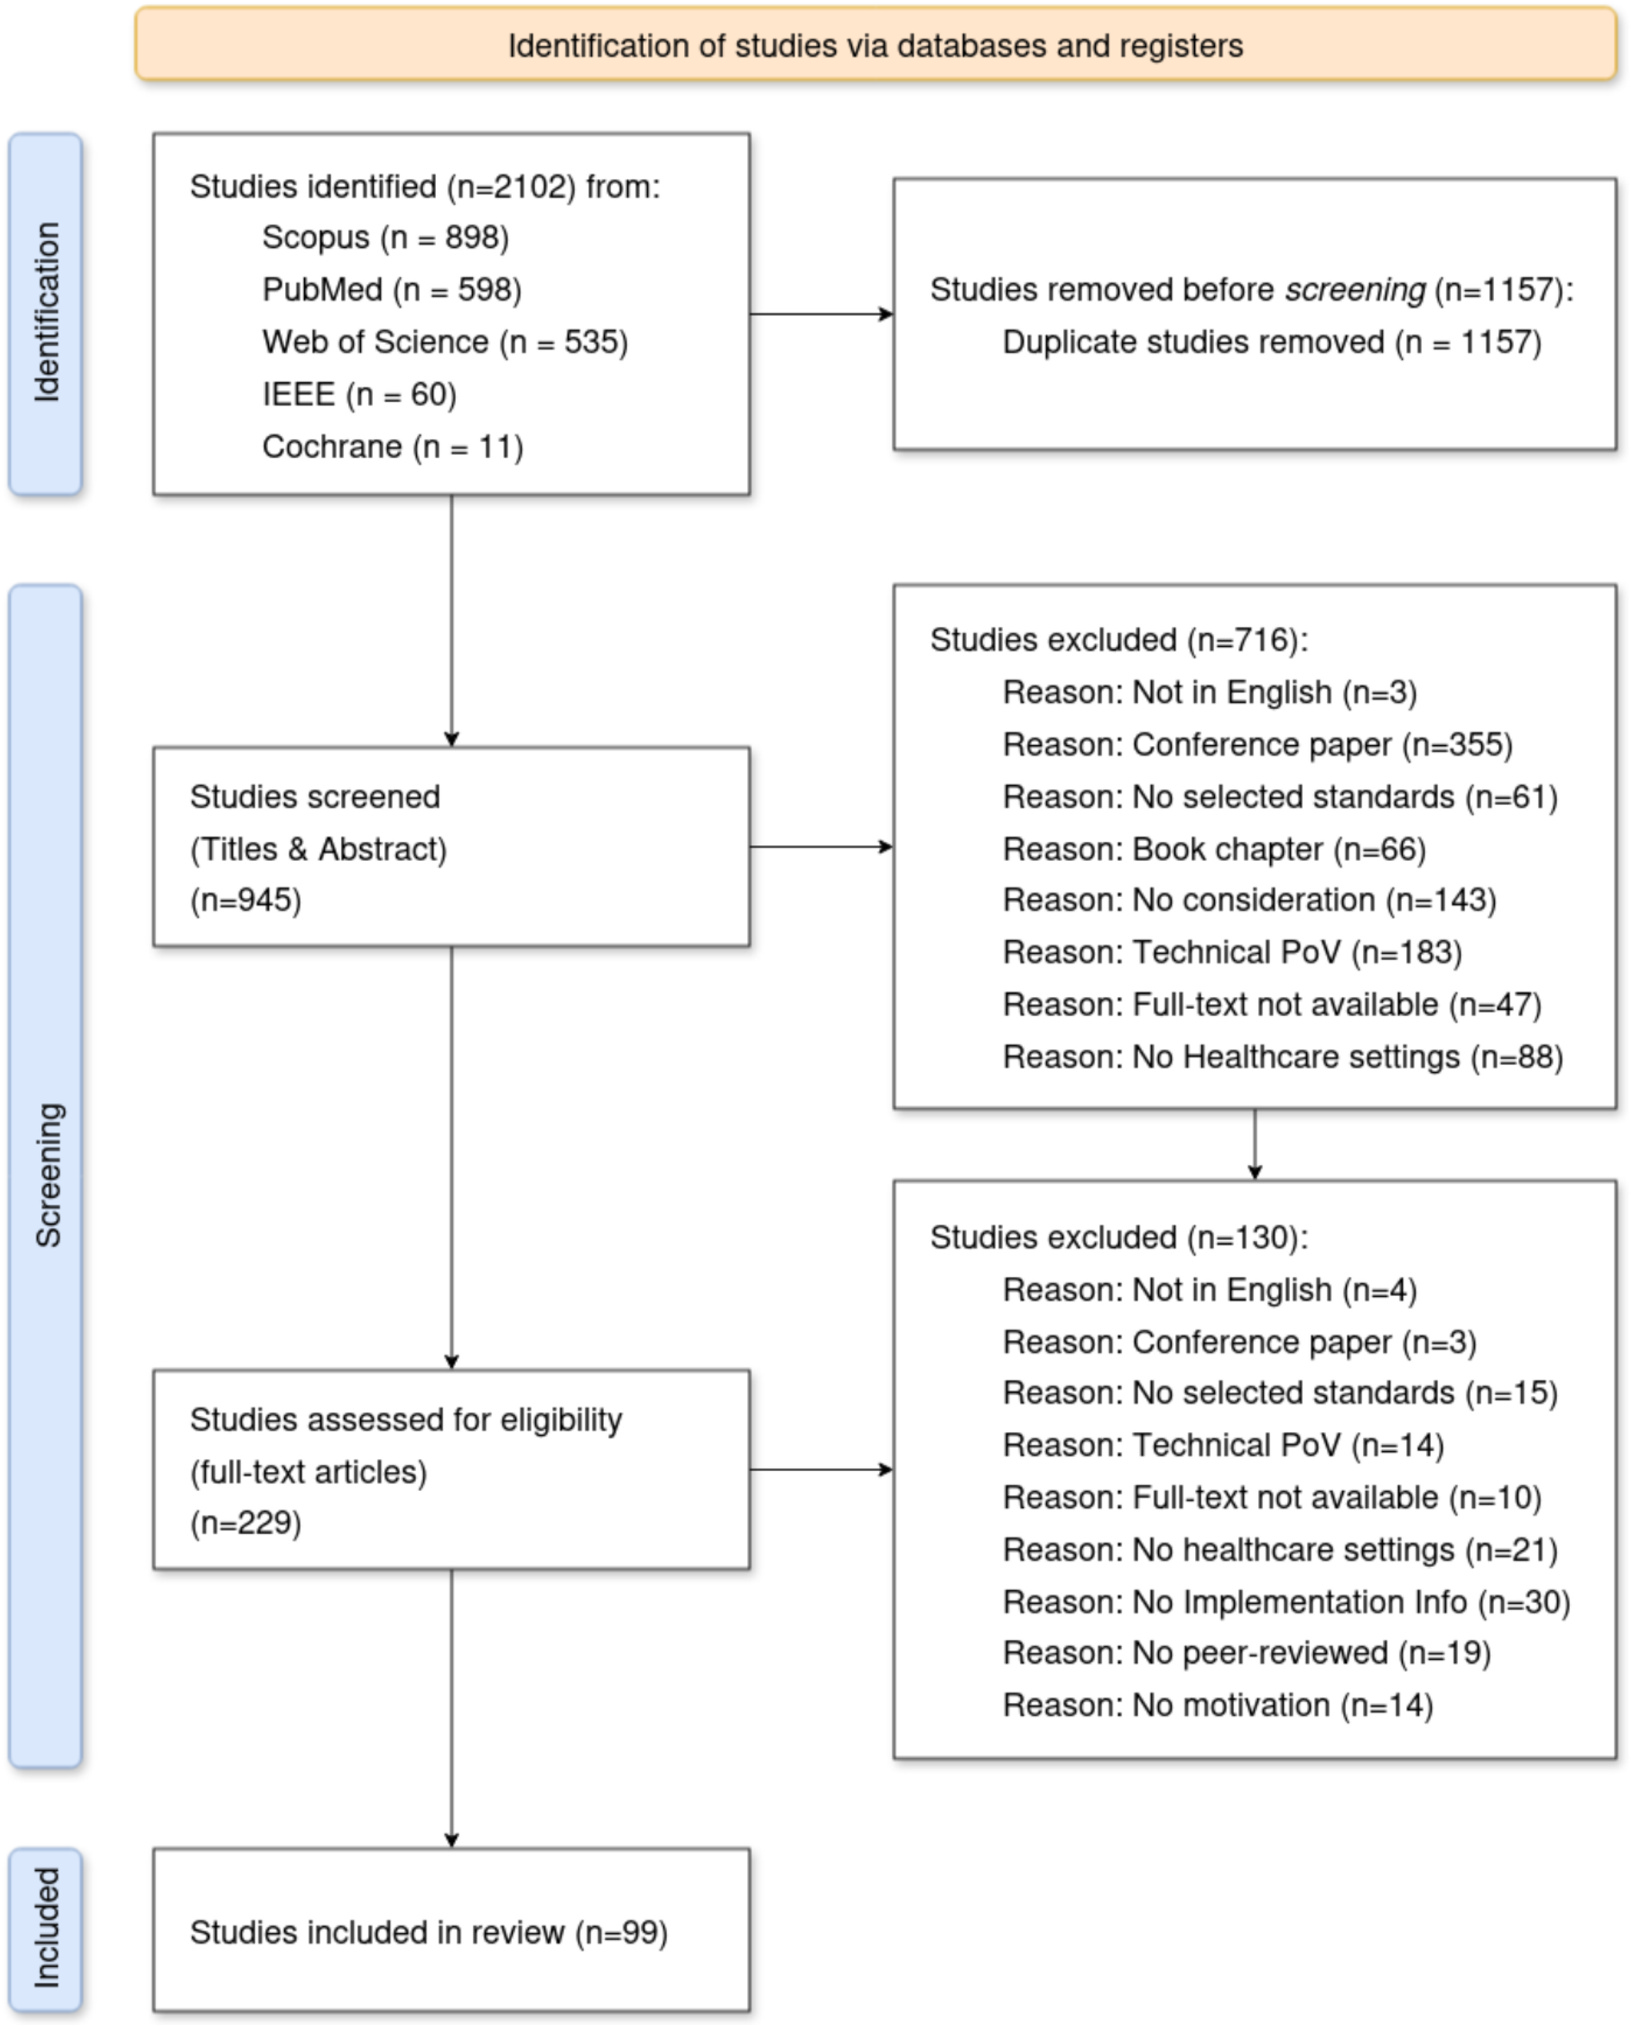
\includegraphics[width=\textwidth]{figures/paper1/fig1-prisma.jpg}
\caption{PRISMA flow diagram illustrating the study selection process, including identification, screening, eligibility assessment, and final inclusion of studies.}
\label{fig:paper1_prisma}
\end{figure}

\subsubsection{Inclusion criteria}
\label{sec:paper1_inclusion_criteria}

The inclusion criteria were as follows: the full text of the article had to be accessible, and the article needed to be available in English. Only studies published in peer-reviewed journals between 2021 and 2024 were considered. The review was limited to peer-reviewed scientific publications to ensure methodological transparency and reproducibility; grey literature and unpublished sources were excluded due to the lack of standardized appraisal frameworks and potential bias.

Eligible studies were required to report on FHIR, OMOP-CDM, or openEHR, to adopt the data standards in real-world or real-like healthcare settings, to discuss the standards from a technical perspective while also considering their practical or organizational aspects for a real-world application, to offer motivation for the use of the selected standards, and to detail how health data standards were adopted, including tools and methods used. The review was intentionally limited to these three standards, as they represent the leading open, community-driven, and freely available health data frameworks, each addressing complementary phases of the data lifecycle \cite{tsafnat_converge_2024}.

We selected 2021 as the starting date for this review as this overlaps with the COVID-19 pandemic, which significantly accelerated the adoption of digital tools. This shift, driven by the urgent need to maintain high-quality healthcare services, was observed both across the European Union and globally \cite{noauthor_repowereu_2022}.

% Paper 1, Table 1 -- transcribed from the published PDF (row order and cell contents as in the PDF text layer).
% Cell text that the PDF continued across a page break has been re-attached to its row (see integration report).
% Layout only: wider margins on the landscape pages of this 99-row table (rows cannot break across pages).
\newgeometry{margin=2cm}
\begin{landscape}
\scriptsize
\setlength{\tabcolsep}{2pt}
\begin{longtable}{>{\raggedright\arraybackslash}p{2.0cm} >{\raggedright\arraybackslash}p{3.8cm} >{\raggedright\arraybackslash}p{1.7cm} >{\raggedright\arraybackslash}p{1.5cm} >{\raggedright\arraybackslash}p{1.3cm} >{\raggedright\arraybackslash}p{7.4cm} >{\raggedright\arraybackslash}p{1.8cm} >{\raggedright\arraybackslash}p{1.3cm} >{\raggedright\arraybackslash}p{1.9cm} >{\raggedright\arraybackslash}p{1.4cm}}
\caption{Summary of extracted data from selected studies, including key characteristics, major application domains, and reported challenges.}
\label{tab:paper1_summary}\\
\toprule
\multicolumn{1}{l}{\textbf{Ref}} & \textbf{Title} & \textbf{Study Location} & \textbf{Health Data Standard} & \textbf{Scale} &
\multicolumn{2}{l}{\textbf{Objective for using the standard}} & \multicolumn{3}{l}{\textbf{Application domain}} \\
 & & & & & \textbf{Detailed} & \textbf{Category} & \textbf{Type} & \textbf{Healthcare Area} & \textbf{Use} \\
\midrule
\endfirsthead
\multicolumn{10}{l}{Table~\ref{tab:paper1_summary} (continued)}\\
\midrule
\multicolumn{1}{l}{\textbf{Ref}} & \textbf{Title} & \textbf{Study Location} & \textbf{Health Data Standard} & \textbf{Scale} &
\multicolumn{2}{l}{\textbf{Objective for using the standard}} & \multicolumn{3}{l}{\textbf{Application domain}} \\
 & & & & & \textbf{Detailed} & \textbf{Category} & \textbf{Type} & \textbf{Healthcare Area} & \textbf{Use} \\
\midrule
\endhead
\midrule
\multicolumn{10}{r}{(continued on next page)}\\
\endfoot
\bottomrule
\endlastfoot
Baumgartner et al., 2024 & Health data space nodes for privacy-preserving linkage of medical data to support collaborative secondary analyses & Austria & OMOP-CDM & National & The primary objective of this study is to propose and evaluate a federated, node-based system architecture called Health Data Space (HDS) nodes to enhance decentralized health data management and analytics. Harmonize heterogeneous data into the OMOP-CDM, which is well-suited for observational health data. & Data Reuse & Research & Clinical Medicine & Secondary \\
Bhattacharjee et al., 2024 & INSPIRE datahub: a pan-African integrated suite of services for harmonising longitudinal population health data using OHDSI tools & Kenya; South Africa; Tanzania & OMOP-CDM & Multi Center & This paper introduces the INSPIRE datahub as a comprehensive solution for data integration and harmonization. Functioning as a pan-African, federated research ecosystem, the datahub is designed to adhere to the principles of FAIR. It tackles critical issues related to reproducibility, standardization, and scalability of data harmonization and sharing systems, primarily in low-resource settings, leveraging existing technologies customized for optimal use. & Data Reuse & Research & Public Health & Secondary \\
Phelan et al., 2024 & Beyond compliance with the 21st Century Cures Act Rule: a patient controlled electronic health information export application programming interface & USA & FHIR & National & The authors formulate a model for interoperable, patient-controlled, app-driven access to EHI exports in an open-source reference implementation following the Argonaut FHIR Accelerator consensus implementation guide for EHI Export. & Data Exchange & Research & Public Health & Secondary \\
Shehab et al., 2024 & The National Healthcare Safety Network's digital quality measures: CDC's automated measures for surveillance of patient safety & USA & FHIR & National & The article outlines NHSN's use of NHSNLink and FHIR APIs to automate public health surveillance via digital quality measures (dQMs), focusing on preventable patient harms like hypoglycemia, C. difficile infection, and venous thromboembolism, piloted through the NHSNCoLab program. & Data Exchange & Clinical & Public Health & Secondary \\
Ulgu et al., 2024 & A Nationwide Chronic Disease Management Solution via Clinical Decision Support Services: Software Development and Real-Life Implementation Report & Turkey & FHIR & National & The DMP (Disease Management Platform) aims to enhance data interoperability with Turkey's central national EHR (e-Nabiz) using HL7 FHIR, allowing data sharing and supporting the screening and monitoring for chronic diseases at the national level. & CDS & Clinical & Clinical Medicine & Secondary \\
Ward et al., 2024 & The OMOP common data model in Australian primary care data: Building a quality research ready harmonised dataset & Australia & OMOP-CDM & National & In this research, the authors aim to investigate the use of the open-source OMOP-CDM in the PATRON primary care data repository. & Data Reuse & Research & Public Health & Secondary \\
Bennett et al., 2023 & MIMIC-IV on FHIR: converting a decade of in-patient data into an exchangeable, interoperable format & Germany; Canada; Netherlands & FHIR & Multi Center & To convert the MIMIC-IV database into FHIR. Additionally, generate and publish an openly available demo of the resources, and create a FHIR Implementation Guide to support and clarify the usage of MIMIC-IV on FHIR. & Data Reuse & Research & Public Health & Secondary \\
Cai et al., 2023 & Advancing Toward a Common Data Model in Ophthalmology & USA & OMOP-CDM & Single Center & To identify gaps in OMOP concept coverage to enhance the standard's ability to accommodate ophthalmology concepts for vision research. & Vocabulary definition & Research & Clinical Services and Diagnostics & Secondary \\
Carus et al., 2023 & Mapping the Oncological Basis Dataset to the Standardized Vocabularies of a Common Data Model: A Feasibility Study & Germany & OMOP-CDM & National & The authors mapped oncological basis dataset (oBDS) elements to the standardized vocabularies, a metadata repository of the observational medical outcomes partnership (OMOP) common data model (CDM). & Data Reuse & Research & Clinical Medicine & Secondary \\
Chechulina et al., 2023 & Semi-Automated Mapping of German Study Data Concepts to an English Common Data Model & Germany & OMOP-CDM & Single Center & To establish a mapping approach that automatically translates German data variable names into English and suggests OMOP concepts. The study focuses on improving the process of mapping medical data from the Hamburg City Health Study (HCHS) to the OMOP-CDM. & Data Reuse & Research & Clinical Medicine & Secondary \\
Mayer et al., 2023 & Learning important common data elements from shared study data: The All of Us program analysis & USA & OMOP-CDM & National & The study aims at gathering different datasets involved in the same national program to identify the common and unique elements within each dataset to guide future study design. & Data Reuse & Research & Public Health & Secondary \\
Dolin et al., 2023 & Sync for Genes Phase 5: Computable artifacts for sharing dynamically annotated FHIR-formatted genomic variants & USA & FHIR & Single Center & The objective of the study is to standardize the sharing of dynamically annotated genetic variants, enabling clinical decision support applications to provide up-to-date, real-time genomic annotations for clinical decision-making. & CDS & Research & Biomedical Sciences & Secondary \\
Einsestein et al., 2023 & Economic Analysis of a Single Institutional Review Board Data Exchange Standard in Multisite Clinical Studies & USA & FHIR & / & The authors conducted a study to determine whether the use of this standard would be economically attractive for sIRB workflows collectively and for Reviewing and Relying institutions. & Data Exchange & Research & Health Information Management & Secondary \\
Espinoza et al., 2023 & Development of an OpenMRS-OMOP ETL tool to support informatics research and collaboration in LMICs & USA & OMOP-CDM & Single Center & To develop a free, open-source ETL pipeline to transform clinical data in OpenMRS instances into OMOP. & Data Reuse & Research & Clinical Medicine & Secondary \\
Guo et al., 2023 & Development and validation of the SickKids Enterprise-wide Data in Azure Repository (SEDAR) & Canada & OMOP-CDM & Single Center & To describe the processes developed by The Hospital for Sick Children (SickKids) to enable utilization of electronic health record (EHR) data by creating sequentially transformed schemas for use across multiple user types. Enable multicenter research and machine learning by adopting the OMOP Common Data Model (CDM), & Data Reuse & Research & Clinical Medicine & Secondary \\
Henke et al., 2023 & Assessing the Use of German Claims Data Vocabularies for Research in the Observational Medical Outcomes Partnership Common Data Model: Development and Evaluation Study & Germany & OMOP-CDM & Multi Center & This study aims to increase the coverage of German vocabularies in the OMOP CDM. & Vocabulary definition & Research & Health Information Management & Secondary \\
Jones et al., 2023 & Real World Performance of the 21st Century Cures Act Population Level Application Programming Interface & USA & FHIR & Multi Center & To evaluate the real-world performance in delivering patient data on populations of the SMART/HL7 Bulk FHIR Access API, required in Electronic Health Records (EHRs) under the 21st Century Cures Act Rule. & Data Exchange & Research & Public Health & Secondary \\
Kempf et al., 2023 & How to Improve Cancer Patients ENrollment in Clinical Trials From rEal-Life Databases Using the Observational Medical Outcomes Partnership Oncology Extension: Results of the PENELOPE Initiative in Urologic Cancers & France & OMOP-CDM & Single Center & The authors wanted to assess the added value of the Oncology Extension of the Observational Medical Outcomes Partnership (OMOP) common data model (CDM) to automatically identify patients with cancer for inclusion in clinical trials (CTs). & CDS & Research & Clinical Medicine & Secondary \\
Kim et al., 2023 & Scalable Infrastructure Supporting Reproducible Nationwide Healthcare Data Analysis toward FAIR Stewardship & South Korea & OMOP-CDM & National & To standardize the national claims data from the HIRA Service of South Korea into the OMOP-CDM, and to build a scalable infrastructure providing accessible and flexible data analysis environments with privacy-by-design protection. & Data Exchange & Research & Health Information Management & Secondary \\
Kiwuwa-Muyingo et al., 2023 & Enabling data sharing and utilization for African population health data using OHDSI tools with an OMOP-common data model & Sub-Saharan Africa & OMOP-CDM & Multi Center & To describe the INSPIRE initiative's innovative approach to data sharing and its efforts to build a FAIR, borderless population health research platform. The paper outlines how this platform leverages OMOP-CDM to facilitate longitudinal population health research and clinical research, with an emphasis on addressing challenges in data sharing within the context of Sub-Saharan Africa (SSA). & CDS & Research & Biomedical Sciences & Secondary \\
Kohler et al., 2023 & Eos and OMOCL: Towards a seamless integration of openEHR records into the OMOP Common Data Model & Germany & OMOP-CDM; openEHR & Multi Center & Both Eos and OMOCL provide a way to define generic mappings for the integration of openEHR records into OMOP. & Data Reuse & Research & Biomedical Sciences & Secondary \\
Mayer, 2023 & Conversion of CPRD AURUM data into the OMOP common data model & UK & OMOP-CDM & National & The author's objective was to convert a static copy of CPRD AURUM data into the OMOP CDM and run existing tools on the converted data. & Data Reuse & Research & Public Health & Secondary \\
Oja et al., 2023 & Transforming Estonian health data to the Observational Medical Outcomes Partnership (OMOP) Common Data Model: Lessons learned & Estonia & OMOP-CDM & National & To describe the reusable process of electronic health records (EHR), claims, and prescriptions data into Observational Medical Outcome Partnership (OMOP) Common Data Model (CDM), together with challenges faced and solutions implemented. & Data Reuse & Research & Health Information Management & Secondary \\
Oliver et al., 2023 & Introducing the BlendedICU dataset, the first harmonized, international intensive care dataset & France & OMOP-CDM & Multi Center & This study introduces the BlendedICU dataset, a massive dataset of international intensive care data. This dataset aims to facilitate generalizability studies of machine learning models, as well as statistical studies of clinical practices in intensive care units. & Data Reuse & Research & Clinical Services and Diagnostics & Secondary \\
Park et al., 2023 & Cancer Research Line (CAREL): Development of Expanded Distributed Research Networks for Prostate Cancer and Lung Cancer & South Korea & OMOP-CDM & Multi Center & The authors attempted to develop DRNs (Distributed Research Networks) for multicenter research that can be easily installed and used by any institution. & Data Reuse & Research & Clinical Medicine & Secondary \\
Peng et al., 2023 & An ETL-process design for data harmonization to participate in international research with German real-world data based on FHIR and OMOP CDM & Germany & FHIR; OMOP-CDM & National & To develop an ETL process that enables German university hospitals to participate in international networks, such as the DARWIN EU project, by: 1. Transforming German patient data from HL7 FHIR to OMOP CDM. 2. Processing large volumes of data efficiently. 3. Ensuring flexibility to accommodate changes in FHIR profiles. & Data Reuse & Research & Public Health & Secondary \\
Rinaldi et al., 2023 & Towards interoperability in infection control: a standard data model for microbiology & Germany & FHIR & National & The objective was to develop a dataset definition, information model, and FHIR® specification for key data elements contained in a German molecular genomics (MolGen) report to facilitate genomic and phenotype integration in electronic health records. & Vocabulary definition & Research & Clinical Medicine & Secondary \\
Raventós et al., 2023 & Transforming the Information System for Research in Primary Care (SIDIAP) in Catalonia to the OMOP Common Data Model and Its Use for COVID-19 Research & Spain & OMOP-CDM & Regional & The primary aim of this work was to convert the Information System for Research in Primary Care (SIDIAP) from Catalonia, Spain, to the Observational Medical Outcomes Partnership (OMOP) Common Data Model (CDM). & Data Reuse & Research & Biomedical Sciences & Secondary \\
Rinaldi et al., 2023 & Towards interoperability in infection control: a standard data model for microbiology & Germany & FHIR & National & The goal is to offer one common format for microbiology data that can be publicly adopted across different institutions and to provide a common international terminology in place of, or together with, the local codes to enhance interoperability. & Vocabulary definition & Research & Clinical Services and Diagnostics & Secondary \\
Sadsad et al., 2023 & A computable biomedical knowledge object for calculating in-hospital mortality for patients admitted with acute myocardial infarction & Australia & OMOP-CDM & National & To calculate in-hospital mortality of patients admitted for acute myocardial infarction (AMI). & CDS & Research & Clinical Medicine & Secondary \\
Seol et al., 2023 & Effect of statin use on head and neck cancer prognosis in a multicenter study using a Common Data Model & South Korea & OMOP-CDM & Multi Center & The authors examined the effect of statin use on HNC recurrence using the converted OMOP-CDM in seven hospitals between 1986 and 2022. & CDS & Research & Clinical Medicine & Secondary \\
Sinaci et al., 2023 & A Data Transformation Methodology to Create Findable, Accessible, Interoperable, and Reusable Health Data: Software Design, Development, and Evaluation Study & Spain & FHIR & Multi Center & To create a methodology for ETL health data into HL7 FHIR repositories following FAIR principles and develop a Data Curation Tool to apply it. & Data Reuse & Research & Public Health & Secondary \\
Song et al., 2023 & Implementation of a Patient Summary Web Application According to the International Patient Summary and Validation in Common Use Cases in Japan & Japan & FHIR & Single Center & This study aimed to develop a patient summary application that summarizes and visualizes patient information accumulated by existing systems. & Data Exchange; Data Reuse & Clinical & Public Health & Primary \\
Tang et al., 2023 & Creating a Medical Imaging Workflow Based on FHIR, DICOMweb, and SVG & Taiwan & FHIR & / & In this study, the authors developed a demonstration system in which FHIR and DICOMweb specifications are used to facilitate the integration of conventional HIS (Hospital Information System) and PACS (Picture Archiving and Communication System). & Data Exchange & Research & Clinical Services and Diagnostics & / \\
Yu et al., 2023 & Integrating real-world data to assess cardiac ablation device outcomes in a multicenter study using the OMOP common data model for regulatory decisions: implementation and evaluation & USA & OMOP-CDM & Multi Center & Describe the application of the Observational Medical Outcomes Partnership (OMOP) common data model (CDM) for supporting medical device real-world evaluation in a National Evaluation System for health Technology Coordinating Center (NESTcc) Test-Case involving two healthcare systems, Mercy Health and Mayo Clinic. & Data Reuse & Research & Clinical Medicine & Secondary \\
Almeida et al., 2022 & BIcenter-AD: Harmonising Alzheimer's Disease cohorts using a common ETL tool & Portugal & OMOP-CDM & Multi Center & The manuscript proposes a collaborative ETL tool designed to harmonize data sources in multi-institutional environments. & Data Reuse & Research & Clinical Medicine & Secondary \\
Bae et al., 2022 & Development of eClaim system for private indemnity health insurance in South Korea: Compatibility and interoperability & South Korea & FHIR & National & This study developed an FHIR®-based electronic claim (eClaim) service to address issues with paper-based workflows, ensuring usability, accessibility, and compatibility with legacy systems. The eClaim service for PIHI has been operational since 2017. & Data Exchange & Clinical & Health Information Management & Primary \\
Bae et al., 2022 & Coronary Artery Computed Tomography Angiography for Preventing Cardio-Cerebrovascular Disease: Observational Cohort Study Using the Observational Health Data Sciences and Informatics' Common Data Model & South Korea & OMOP-CDM & Single Center & The objective of the study was to investigate the effectiveness of Coronary artery computed tomography angiography (CCTA) screening on Cardio-cerebrovascular diseases (CVDs) outcomes by using the OMOP-CDM data and the population-level estimation method. & CDS & Research & Clinical Medicine & Secondary \\
Bathelt et al., 2022 & Opportunities of Digital Infrastructures for Disease Management---Exemplified on COVID-19-Related Change in Diagnosis Counts for Diabetes-Related Eye Diseases & Germany & OMOP-CDM & Multi Center & To demonstrate (1) how to facilitate digital infrastructures to run a retrospective study in a research network spread across university and non-university hospital sites; and (2) to answer a medical question on COVID-19 related change in diagnostic counts for diabetes-related eye diseases. & Data Reuse & Research & Biomedical Sciences & Secondary \\
Bialke et al., 2022 & A FHIR has been lit on gICS: facilitating the standardised exchange of informed consent in a large network of university medicine & Germany & FHIR & Multi Center & To implement a standardized solution for the FHIR-compliant provision of consent information using gICS. & Data Exchange & Research & Health Information Management & Secondary \\
Bradshaw et al., 2022 & GARDE: a standards-based clinical decision support platform for identifying population health management cohorts & USA & FHIR & Multi Center & To design and implement a scalable standards-based clinical decision support (CDS) approach to identify patient cohorts for PHM and maximize opportunities for multi-site dissemination. & CDS & Clinical & Clinical Medicine & Primary \\
Byun et al., 2022 & Analysis of treatment pattern of anti-dementia medications in newly diagnosed Alzheimer's dementia using OMOP CDM & Korea & OMOP-CDM & Multi Center & OMOP CDM was used for standardized, large-scale, multi-center analysis of AD treatment. & CDS & Research & Clinical Medicine & Secondary \\
Carus et al., 2022 & Mapping Cancer Registry Data to the Episode Domain of the Observational Medical Outcomes Partnership Model (OMOP) & Germany & OMOP-CDM & National & The objective of this study was firstly to find out to what extent the source terminologies of the clinical cancer registry can be mapped to the respective OMOP standard. & Vocabulary definition & Research & Clinical Medicine & Secondary \\
Castano et al., 2022 & Identification of patients with drug-resistant epilepsy in electronic medical record data using the Observational Medical Outcomes Partnership Common Data Model & USA & OMOP-CDM & Single Center & The authors aim to develop and compare the performance of computable phenotypes for drug-resistant epilepsy (DRE) using the OMOP Common Data Model. & CDS & Research & Clinical Medicine & Secondary \\
Choi et al., 2022 & Conversion of Automated 12-Lead Electrocardiogram Interpretations to OMOP CDM Vocabulary & South Korea & OMOP-CDM & Multi Center & The authors aim to develop a fully automated text data conversion algorithm that overcomes the limitations of existing tools and manual conversion. & Data Reuse; Vocabulary definition & Research & Clinical Medicine & Secondary \\
Chukwu et al., 2022 & Standardizing Primary Health Care Referral Data Sets in Nigeria: Practitioners' Survey, Form Reviews, and Profiling of Fast Healthcare Interoperability Resources (FHIR) & Nigeria & FHIR & Regional & The objective of this study is to design FHIR profiles and present methodology and the profiled FHIR resource for Maternal and Child Health referral use cases in Ebonyi state, Nigeria---a typical low- and middle-income country (LMIC) setting. & Vocabulary definition & Research & Clinical Medicine & Secondary \\
Delanerolle et al., 2022 & Methodological Issues in Using a Common Data Model of COVID-19 Vaccine Uptake and Important Adverse Events of Interest: Feasibility Study of Data and Connectivity COVID-19 Vaccines Pharmacovigilance in the United Kingdom & UK & OMOP-CDM & National & This study aims to use the concept mappings in the OMOP-CDM to identify common concepts recorded and to report these in a repeated cross-sectional study. & Data Reuse & Research & Biomedical Sciences & Secondary \\
Gruendner et al., 2022 & The Architecture of a Feasibility Query Portal for Distributed COVID-19 Fast Healthcare Interoperability Resources (FHIR) Patient Data Repositories: Design and Implementation Study & Germany & FHIR & National & This study described the design and implementation of the components involved in creating a cross-hospital feasibility query platform for researchers based on FHIR resources. This effort was part of a large COVID-19 data exchange platform and was designed to be scalable for a broad range of patient data. & CDS;Data Exchange & Research & Biomedical Sciences & Secondary \\
Jung et al., 2022 & Patient-Level Fall Risk Prediction Using the Observational Medical Outcomes Partnership's Common Data Model: Pilot Feasibility Study & South Korea & OMOP-CDM & Single Center & The objectives of this study were to (1) convert fall-related electronic health record data into OMOP common data model format and (2) develop models that predict fall risk during 2 time periods. & CDS & Research & Clinical Medicine & Secondary \\
Jung et al., 2022 & Shared Interoperable Clinical Decision Support Service for Drug-Allergy Interaction Checks: Implementation Study & South Korea & FHIR & National & The study focuses on developing and deploying the national CDS service for drug-allergy interaction (DAI) to check for healthcare providers in Korea which need to introduce the service but lack the budget and expertise. & CDS;Data Exchange & Clinical & Clinical Services and Diagnostics & Secondary \\
Junior et al., 2022 & Integrating real-world data from Brazil and Pakistan into the OMOP common data model and standardized health analytics framework to characterize COVID-19 in the Global South & Pakistan; Brazil & OMOP-CDM & Multi Center & This work aims to demonstrate the use of a standardized health informatics framework to generate reliable and reproducible real-world evidence from Latin America and South Asia towards characterizing coronavirus disease 2019 (COVID-19) in the Global South. & Data Reuse & Research & Biomedical Sciences & Secondary \\
K Sommer et al., 2022 & Structured, Harmonized, and Interoperable Integration of Clinical Routine Data to Compute Heart Failure Risk Scores & Germany & openEHR & Multi Center & To demonstrate the feasibility of deriving and calculating heart failure (HF) risk scores (MAGGIC and Barcelona Bio-HF) from clinical routine data using an interoperable, harmonized core dataset within the openEHR framework. & CDS & Research & Clinical Medicine & Secondary \\
Lazarova et al., 2022 & An Interoperable Electronic Health Record System for Clinical Cardiology & Italy & FHIR & Regional & The main aim of the project is to design, produce, deploy, and test a new modular electronic health record system (EHRS) to be used in the cardiological wards of some local hospitals. The main objective has been to replace the paper-based system. & Data Exchange; EHR Design & Clinical & Clinical Medicine & Primary \\
Li et al., 2022 & A configurable method for clinical quality measurement through electronic health records based on openEHR and CQL & China & openEHR & Single Center & To help clinical staff develop clinical quality indicators to monitor and improve the performance and quality of healthcare services. & CDS & Clinical & Clinical Medicine & Secondary \\
McGuinness et al., 2022 & Extraction of Electronic Health Record Data using Fast Healthcare Interoperability Resources for Automated Breast Cancer Risk Assessment & USA & FHIR & Single Center & To discuss the development of web-based tools for breast cancer risk assessment, barriers to their use, and the potential for automating risk calculations using FHIR to improve patient care and decision-making. & CDS & Research & Clinical Medicine & Secondary \\
Papez et al., 2022 & Transforming and evaluating electronic health record disease phenotyping algorithms using the OMOP common data model: a case study in heart failure & UK & OMOP-CDM & Multi Center & The authors' objective was to convert the UK Biobank, a study of 500 000 participants with rich genetic and phenotypic data to the Observational Medical Outcomes Partnership (OMOP) CDM. & Data Reuse & Research & Public Health & Secondary \\
Phuong et al., 2022 & Extracting Patient-level Social Determinants of Health into the OMOP Common Data Model & USA & OMOP-CDM & Multi Center & This paper uses the University of Washington Enterprise Data Warehouse (a data contributor to N3C) to demonstrate how SDoH can be represented and managed to be made available within an OMOP common data model. & Data Reuse & Research & Biomedical Sciences & Secondary \\
Román-Villarán et al., 2022 & A Personalized Ontology-Based Decision Support System for Complex Chronic Patients: Retrospective Observational Study & Spain & FHIR & Multi Center & To design, develop, and validate an ontology-based CDSS that provides personalized recommendations related to drug prescription. & CDS & Research & Clinical Medicine & Secondary \\
Rosenau et al., 2022 & Generation of a Fast Healthcare Interoperability Resources (FHIR)-based Ontology for Federated Feasibility Queries in the Context of COVID-19: Feasibility Study & Germany & FHIR & National & This study investigates how search ontology can be automatically generated using FHIR profiles and a terminology server. Furthermore, it describes how this ontology can be used in a user interface (UI) and how a mapping and a terminology tree created together with the ontology can translate user input into FHIR queries. & Vocabulary definition & Research & Biomedical Sciences & Secondary \\
Spotnitz et al., 2022 & Patient characteristics and antiseizure medication pathways in newly diagnosed epilepsy: Feasibility and pilot results using the common data model in a single-center electronic medical record database & USA & OMOP-CDM & Single Center & To demonstrate the feasibility of characterizing adult patients with epilepsy and ASM treatment pathways using the CDM in an electronic health record (EHR)-derived database. & CDS & Research & Clinical Medicine & Secondary \\
Wang et al., 2022 & The sociodemographic characteristics and clinical features of the late-life depression patients: results from the Beijing Anding Hospital mental health big data platform & China & OMOP-CDM & Single Center & This study aimed to explore the psychiatric outpatient attendance of LLD (late-life depression) patients at a psychiatric hospital in China, with a subgroup analysis, such as with or without anxiety, gender differences. & CDS & Research & Clinical Medicine & Secondary \\
Xing Tan et al., 2022 & Applying the OMOP Common Data Model to Facilitate Benefit-Risk Assessments of Medicinal Products Using Real-World Data from Singapore and South Korea & Singapore; South Korea & OMOP-CDM & Multi Center & The aim of this study was to characterize the potential usefulness of CDM conversion by conducting a sample benefit-risk assessment involving CDM-converted data. & CDS; Data Reuse & Research & Clinical Medicine & Secondary \\
Yoo et al., 2022 & Transforming Thyroid Cancer Diagnosis and Staging Information from Unstructured Reports to the Observational Medical Outcome Partnership Common Data Model & South Korea & OMOP-CDM & Multi Center & The authors aimed to demonstrate the applicability of the OMOP CDM oncology extension module for thyroid cancer diagnosis and cancer stage information by processing free-text medical reports. & Data Reuse & Research & Clinical Medicine & Secondary \\
Yu et al., 2022 & Developing an ETL tool for converting the PCORnet CDM into the OMOP CDM to facilitate the COVID-19 data integration & USA & OMOP-CDM & Single Center & The objective of this study is to design, develop, and evaluate an ETL tool that transforms the PCORnet CDM format data into the OMOP CDM. & Data Reuse & Research & Biomedical Sciences & Secondary \\
Almeida et al., 2021 & A methodology for cohort harmonisation in multicentre clinical research & Portugal & OMOP-CDM & Multi Center & To present a methodology to extract relevant concepts from clinical notes to enrich structured OMOP CDM databases, enabling the use of SQL queries for analyzing clinical text information. & Data Reuse & Research & Clinical Services and Diagnostics & Secondary \\
Almeida et al., 2021 & A two-stage workflow to extract and harmonize drug mentions from clinical notes into observational databases & Germany; Netherlands & OMOP-CDM & Multi Center & To harmonize different cohorts into a standard data schema, facilitating multi-cohort querying and analysis. & Data Reuse; Data Exchange & Research & Clinical Medicine & Secondary \\
Biedermann et al., 2021 & Standardizing registry data to the OMOP Common Data Model: experience from three pulmonary hypertension databases & USA;Europe and Canada & OMOP-CDM & Multi Center & The study objective is to document the process and outcomes of transforming registry data in PH (Pulmonary Hypertension) to the OMOP CDM, highlighting challenges and providing potential solutions. & Data Reuse & Research & Clinical Medicine & Secondary \\
Carvalho Gomes et al., 2021 & Representation of Diagnosis and Nursing Interventions in OpenEHR Archetypes & Brazil & openEHR & Single Center & The study aimed to represent the content of nursing diagnosis and interventions in the openEHR standard. & EHR Design & Research & Clinical Services and Diagnostics & Secondary \\
De et al., 2021 & Analyzing Patient Secure Messages Using a Fast Health Care Interoperability Resources (FIHR)-Based Data Model: Development and Topic Modeling Study & USA & FHIR & Single Center & To develop a data model for patient secure messages based on the FHIR standard to extract significant information. & Vocabulary definition & Research & Public Health & Secondary \\
Dolin et al., 2021 & Sync for Genes Phase 5: Computable artifacts for sharing dynamically annotated FHIR-formatted genomic variants & USA & FHIR & National & To describe an open-source utility for converting variants from VCF format into HL7 FHIR format & Data Exchange & Research & Biomedical Sciences & Secondary \\
González-Castro et al., 2021 & CASIDE: A data model for interoperable cancer survivorship information based on FHIR & Spain & FHIR & Multi Center & To present CASIDE, an interoperable data model for cancer survivorship information that aims to accelerate the secondary use of healthcare data and data sharing across institutions. It is designed to provide a holistic view of the cancer survivor, taking into account not just the clinical data but also the patient's own perspective, and is built upon the emerging FHIR standard. & Data Reuse; Vocabulary definition & Research & Clinical Medicine & Secondary \\
Gruendner et al., 2021 & The Architecture of a Feasibility Query Portal for Distributed COVID-19 Fast Healthcare Interoperability Resources (FHIR) Patient Data Repositories: Design and Implementation Study & Germany & FHIR & Single Center & To elucidate how FHIR data can be queried directly with a preprocessing service and be used for statistical analyses. & Data Reuse & Research & Public Health & Secondary \\
Guinez-Molinos et al., 2021 & Interoperable Platform to Report Polymerase Chain Reaction SARS-CoV-2 Tests From Laboratories to the Chilean Government: Development and Implementation Study & Chile & FHIR & Single Center & This study aims to design and develop an interoperable platform to report polymerase chain reaction (PCR) SARS-CoV-2 tests from laboratories to the Chilean government. & Data Exchange & Clinical & Biomedical Sciences & Secondary \\
Gulden et al., 2021 & Prototypical Clinical Trial Registry Based on Fast Healthcare Interoperability Resources (FHIR): Design and Implementation Study & Germany & FHIR & Multi Center & This study investigates how Health Level 7 (HL7) Fast Healthcare Interoperability Resources (FHIR) may be used as a standardized format for exchanging and storing clinical trial records. & Data Exchange & Research & Health Information Management & Secondary \\
Kawamoto et al., 2021 & Establishing a multidisciplinary initiative for interoperable electronic health record innovations at an academic medical center & USA & FHIR & Multi Center & To establish an enterprise initiative for improving health and health care through interoperable electronic health record (EHR) innovations. & EHR Design & Clinical & Public Health & Primary \\
Khalifa et al., 2021 & Interoperable genetic lab test reports: mapping key data elements to HL7 FHIR specifications and professional reporting guidelines & USA & FHIR & Single Center & This study aims to identify various data content of some genetic lab test reports and map them to FHIR CG IG specifications to assess its coverage and to provide some suggestions for standard development and implementation. & Vocabulary definition & Research & Biomedical Sciences & Secondary \\
Kim et al., 2021 & Transforming electronic health record polysomnographic data into the Observational Medical Outcome Partnership's Common Data Model: a pilot feasibility study & South Korea & OMOP-CDM & Multi Center & The study aimed to assess the link between irritable bowel syndrome (IBS) medications and the risk of osteoporosis and fractures. & CDS & Research & Clinical Medicine & Secondary \\
Kim et al., 2021 & The Risk of Osteoporosis and Osteoporotic Fracture Following the Use of Irritable Bowel Syndrome Medical Treatment: An Analysis Using the OMOP CDM Database & South Korea & OMOP-CDM & Single Center & To convert EHR PSG into a standardized data format---the OMOP-CDM. The authors designed and implemented an extract--transform--load (ETL) process to transform PSG data into the OMOP-CDM format and verified the data quality through expert evaluation. & Data Reuse & Research & Clinical Services and Diagnostics & Secondary \\
Lamer et al., 2021 & Transforming Anesthesia Data into the Observational Medical Outcomes Partnership Common Data Model: Development and Usability Study & France & OMOP-CDM & Multi Center & The primary objective was to transform anesthesia data into the OMOP-CDM. The secondary objective was to provide vocabulary, queries, and dashboards that might promote the exploitation and sharing of anesthesia data through the CDM. & Data Reuse & Research & Clinical Services and Diagnostics & Secondary \\
Lenert et al., 2021 & Transforming Anesthesia Data into the Observational Medical Outcomes Partnership Common Data Model: Development and Usability Study & USA & FHIR; OMOP-CDM & Single Center & To describe the use of the FHIR data model as a canonical data model and the automated transformation of clinical data to PCORnet and OMOP CDMs for data sharing and research collaboration on COVID-19. & Data Reuse; Data Exchange & Research & Biomedical Sciences & Secondary \\
Li et al., 2021 & Automated production of research data marts from a canonical fast healthcare interoperability resource data repository: applications to COVID-19 research & China & openEHR & Single Center & The study aims to develop a patient-screening tool based on EHRs for clinical research using openEHR to solve concept mismatches and improve query performance. & Data Reuse & Research & Clinical Medicine & Secondary \\
Mishra et al., 2021 & A Modified Public Health Automated Case Event Reporting Platform for Enhancing Electronic Laboratory Reports With Clinical Data: Design and Implementation Study & USA & FHIR & Single Center & To present a pilot implementation of a modified PACER system for electronic case reporting that allows health systems to conduct public health reporting while maintaining the appropriate governance of the clinical data. & Data Exchange & Clinical & Public Health & Secondary \\
Mun et al., 2021 & Real-world incidence of endopthalmitis after intravitreal anti-VEGF injections in Korea: findings from the Common Data Model in ophthalmology & South Korea & OMOP-CDM & Multi Center & The aim of this study was to evaluate the real-world incidence of endophthalmitis after intravitreal anti-vascular endothelial growth factor (VEGF) injections using data from the OMOP-CDM. & CDS & Research & Clinical Services and Diagnostics & Secondary \\
Nestsiarovich et al., 2021 & Predictors of diagnostic transition from major depressive disorder to bipolar disorder: a retrospective observational network study & USA; South Korea;UK & OMOP-CDM & Multi Center & To develop and validate a predictive model for identifying patients with major depressive disorder (MDD) who are at risk of converting to bipolar disorder (BD). The study aims to address the diagnostic challenge of distinguishing MDD as a potential early stage of BD versus a comorbidity, thereby enabling earlier recognition and treatment of BD & CDS & Research & Clinical Medicine & Secondary \\
Oliveira et al., 2021 & OpenEHR modeling: improving clinical records during the COVID-19 pandemic & Portugal & openEHR & Single Center & To develop and integrate an openEHR-based approach to improve interoperability with existing information systems at the CHUP healthcare institution, in response to the challenges posed by the COVID-19 pandemic. & EHR Design & Research & Biomedical Sciences & Secondary \\
Papez et al., 2021 & Transforming and evaluating electronic health record disease phenotyping algorithms using the OMOP common data model: a case study in heart failure & UK & OMOP-CDM & Multi Center & The study aimed to transform a resource of linked electronic health records (EHR) to the OMOP common data model (CDM) and evaluate the process in terms of syntactic and semantic consistency and quality when implementing disease and risk factor phenotyping algorithms. & Data Reuse & Research & Clinical Medicine & Secondary \\
Paris et al., 2021 & Transformation and Evaluation of the MIMIC Database in the OMOP Common Data Model: Development and Usability Study & France & OMOP-CDM & Single Center & The objective was to transform MIMIC into an OMOP database and to evaluate the benefits of this transformation for analysts. & Data Reuse & Research & Clinical Services and Diagnostics & Secondary \\
Park et al., 2021 & A Worker-Centered Personal Health Record App for Workplace Health Promotion Using National Health Care Data Sets: Design and Development Study & Korea & FHIR & National & Using Fast Healthcare Interoperability Resources (FHIR) and national health care data sets, this study aimed to design and develop an app for providing worker-centered, interconnected PHR services. & EHR Design; Data Exchange & Research & Public Health & Secondary \\
Sathappan et al., 2021 & Transformation of Electronic Health Records and Questionnaire Data to OMOP CDM: A Feasibility Study Using SG\_T2DM Dataset & Singapore & OMOP-CDM & National & The study aimed to evaluate the feasibility of converting Singapore based data source, comprising of electronic health records (EHR), cognitive and depression assessment questionnaire data to OMOP-CDM standard. & Data Reuse & Research & Health Information Management & Secondary \\
Seong et al., 2021 & Fast Healthcare Interoperability Resources (FHIR)--Based Quality Information Exchange for Clinical Next-Generation Sequencing Genomic Testing: Implementation Study & South Korea & FHIR & Single Center & The goal of this study was to develop a Fast Healthcare Interoperability Resources (FHIR)--based web app, NGS Quality Reporting (NGS-QR), to report and manage the quality of the information obtained from clinical NGS genomic tests. & Data Exchange & Research & Biomedical Sciences & Secondary \\
Seong et al., 2021 & Incorporation of Korean Electronic Data Interchange Vocabulary into Observational Medical Outcomes Partnership Vocabulary & South Korea & OMOP-CDM & National & The authors incorporated the Korean Electronic Data Interchange (EDI) vocabulary into Observational Medical Outcomes Partnership (OMOP) vocabulary using a semi-automated process. The goal of this study was to improve the Korean EDI as a standard medical ontology in Korea. & Vocabulary definition & Research & Public Health & Secondary \\
Sun et al., 2021 & Building an OMOP common data model-compliant annotated corpus for COVID-19 clinical trials & USA & OMOP-CDM & National & To develop COVIC, a semi-automatic annotated corpus based on the OMOP Common Data Model, to make COVID-19 clinical trial eligibility criteria computable, thereby facilitating automated eligibility screening and enhancing trial search and analytics. & Data Reuse & Research & Biomedical Sciences & Secondary \\
Thayer et al., 2021 & Human-centered development of an electronic health record-embedded, interactive information visualization in the emergency department using fast healthcare interoperability resources & USA & FHIR & Single Center & To develop and evaluate an interactive information visualization embedded within the electronic health record (EHR) by following human-centered design (HCD) processes and leveraging modern health information exchange standards. & EHR Design & Clinical & Clinical Medicine & Primary \\
Tian et al., 2021 & Application of openEHR archetypes to automate data quality rules for electronic health records: a case study & China & openEHR & Single Center & To automatically create DQRs (automating data quality rules) based on openEHR archetypes to investigate the feasibility and challenges of automating DQA (data quality assessment) for EHR data. & Data Reuse & Research & Health Information Management & Secondary \\
Wesley et al., 2021 & A novel application of SMART on FHIR architecture for interoperable and scalable integration of patient-reported outcome data with electronic health records & USA & FHIR & Multi Center & Despite many apps for collecting patient-reported outcomes (PROs), integrating this data into EHRs remains challenging. Using new PRO standards, researchers developed an architecture to integrate PRO data seamlessly across EHRs in outpatient settings using FHIR-compatible apps. & Data Exchange; Data Reuse & Clinical & Public Health & Primary \\
Khalid et al., 2021 & A standardized analytics pipeline for reliable and rapid development and validation of prediction models using observational health data & USA; South Korea;Spain & OMOP-CDM & Multi Center & To present the OHDSI analytics pipeline for patient-level prediction modeling as a standardized approach for rapid yet reliable development and validation of prediction models. & Data Reuse & Research & Biomedical Sciences & Secondary \\
Wulff et al., 2021 & Transformation of microbiology data into a standardised data representation using OpenEHR & Germany & openEHR & Multi Center & To present a multi-centric standardization approach by using openEHR as modelling standard. & Data Reuse & Research & Clinical Services and Diagnostics & Secondary \\
Xiao et al., 2021 & Development of an application concerning fast healthcare interoperability resources based on standardized structured medical information exchange version 2 data & Japan & FHIR & Single Center & This study aims to convert clinical data in EHRs into the Health Level Seven (HL7) Fast Healthcare Interoperability Resources (FHIR) data format while developing a PHR application to present the FHIR data. & Data Exchange & Research & Public Health & Primary \\
Zong et al., 2021 & Modeling Cancer Clinical Trials Using HL7 FHIR to Support Downstream Applications: A Case Study with Colorectal Cancer Data & USA & FHIR & Single Center & To develop a methodology to comprehensively capture the clinical trial data element needs by identifying and standardizing data elements used in clinical trials. This aims to reduce costs and errors in the operational process and enable seamless data exchange between Electronic Data Capture (EDC) systems and Electronic Health Record (EHR) systems. & Data Exchange & Research & Clinical Medicine & Secondary \\
\end{longtable}
\end{landscape}
\restoregeometry


\begin{figure}[tbp]
\centering
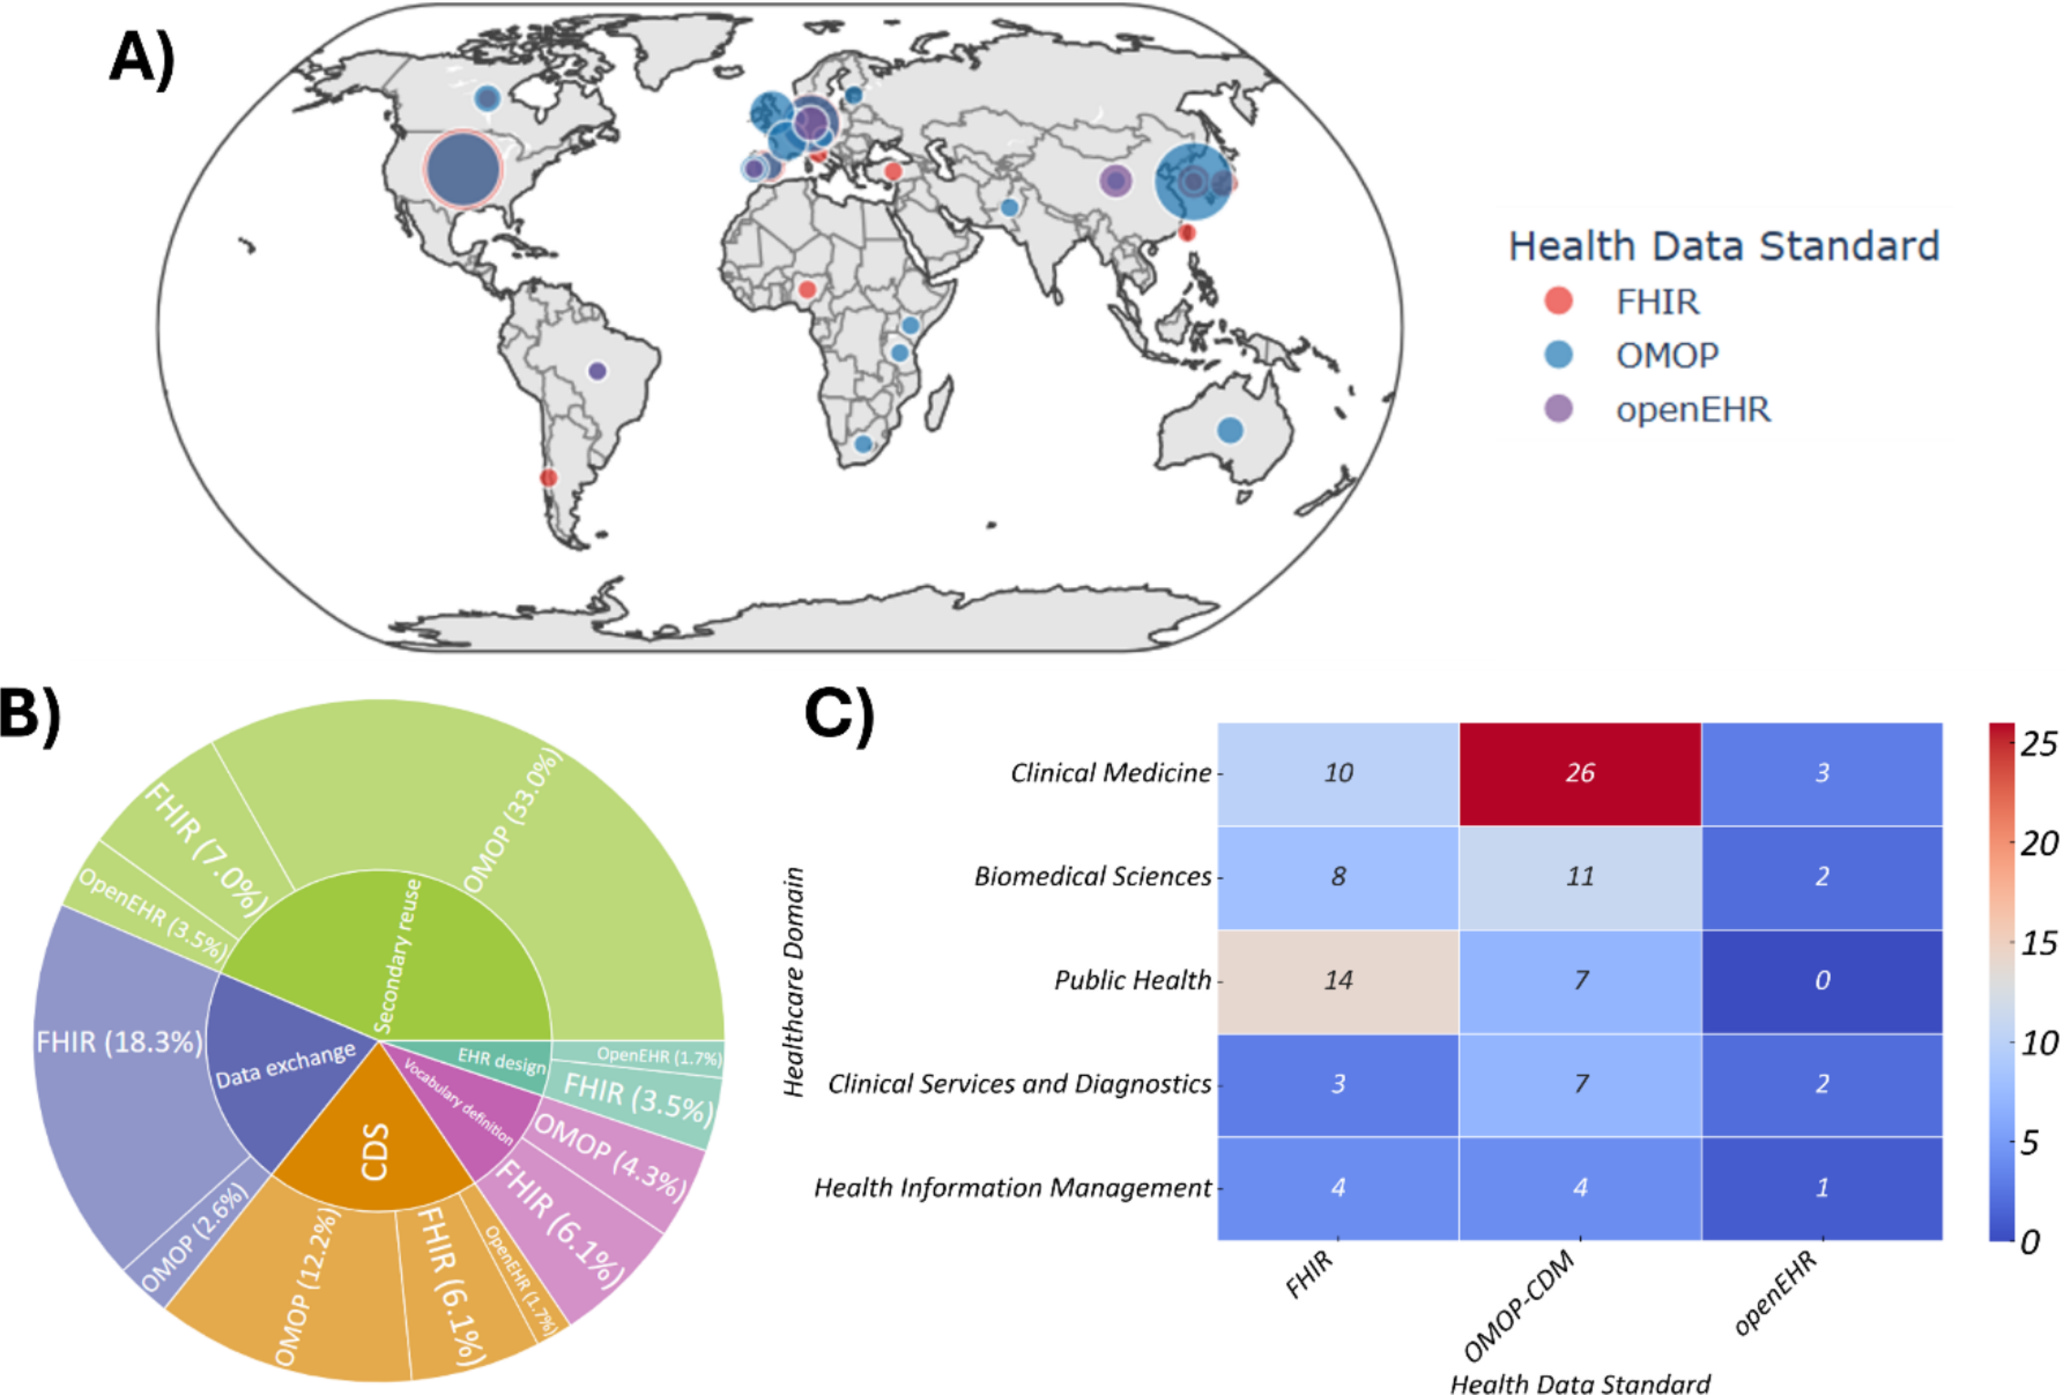
\includegraphics[width=\textwidth]{figures/paper1/fig2-overview.jpg}
\caption{Overview of the included studies A) Geographical distribution B) Distribution of the objectives, divided for each health data standard C) Healthcare domain in which health data standards are applied.}
\label{fig:paper1_overview}
\end{figure}

\subsubsection{Data extraction}
\label{sec:paper1_data_extraction}

The primary objective of this research was to outline the application of major health data standards (i.e., FHIR, OMOP-CDM, and openEHR) for real-world applications. To achieve this, we identified five key categories to clarify the context in which health data standards are used. These categories are defined as follows:

\begin{itemize}
  \item Data Exchange: The seamless transfer of health information between different systems or organizations while ensuring data accuracy, security, and interoperability.
  \item Clinical Decision Support: Enhancing clinical workflows by providing tools and recommendations to assist healthcare professionals in making informed decisions.
  \item Vocabulary Definition: Establishing terminologies and codes to ensure consistency in the representation and interpretation of clinical and administrative data.
  \item Data Reuse: Leveraging health data previously collected for patient care to pursue secondary objectives such as research, quality improvement, and public health surveillance.
  \item EHR Design: Structuring and developing electronic health records to ensure efficient data capture, usability, and interoperability.
\end{itemize}

Furthermore, we identified five major health application domains in the included studies, which were used to categorize the reviewed literature:

\begin{itemize}
  \item[i)] Clinical Medicine, including all studies about clinical and their respective applications.
  \item[ii)] Clinical Services and Diagnostics, covering studies related to healthcare delivery processes, diagnostic methodologies, and technology-supported clinical care.
  \item[iii)] Public Health, including epidemiological studies, health surveillance, and population health management.
  \item[iv)] Health Information Management, addressing data governance, interoperability frameworks, and data standardization strategies.
  \item[v)] Biomedical Sciences, focusing on bioinformatics, translational research, and the integration of health data into biomedical research.
\end{itemize}

Data extraction was led by the first author (AM), who coordinated the process and harmonized the results, with active participation from the full team in defining categories, reviewing data, and resolving ambiguities. Category selections were iteratively refined through team discussions before AM finalized the structure. Studies identified as eligible for this review have been synthesized using tables and figures to facilitate a clear understanding of the key findings. The study characteristics and outcome data will be presented in tables, resulting in aggregated information about i) General overview of the studies, ii) Dataset characteristics, iii) adopted ETL tools, and iv) Data Standard Maturity and Adoption.

\subsection{Results}
\label{sec:paper1_results}

From the systematic query of the five scientific databases, a total of 2102 records were retrieved. Before the title and abstract screening, we removed 1157 duplicate entries. Subsequently, 945 studies underwent title and abstract screening, removing a total of 716 records because they did not meet the inclusion criteria. The remaining 229 records were assessed based on their full text. Finally, 99 studies met all the inclusion criteria and were selected for further analysis. The PRISMA diagram in Fig.~\ref{fig:paper1_prisma} illustrates the complete study selection process.

Table~\ref{tab:paper1_summary} provides an overview of the included studies, specifying the study location, the standard the article is focused on, the scale at which the standardization procedure was applied, and the authors' stated objectives for applying the standard, both as described in natural language as reported in the article and as classified into the five categories defined in this review; lastly, the table includes information regarding the standard application domain, specifying if the standardization was implemented for research or clinical purposes, the health domain concerning the standardization procedure, and whether the application involved primary or secondary data use.

To enhance transparency and enable sorting and filtering of the data, the full version of Table~\ref{tab:paper1_summary} has been deposited on Zenodo. The repository \cite{marfoglia_challenges_data_2026} includes Table 1\_extended, containing the complete data extraction with detailed annotations, as well as Table 1\_summary, corresponding to the condensed version presented in the manuscript.

\subsubsection{What are the main characteristics and applications of standardized health data?}
\label{sec:paper1_results_characteristics}

The included studies were conducted across different geographical locations (Fig.~\ref{fig:paper1_overview}A), with a significant presence of high-income countries (i.e., United States, Germany, Korea, Japan). In terms of implementation scale, 31 studies \cite{li_configurable_2022,cai_advancing_2023,chechulina_semi-automated_2023,dolin_sync_2023,espinoza_development_2023,guo_development_2023,kempf_how_2023,song_implementation_2023,bae_coronary_2022,castano_identification_2022,jung_patient-level_2022,mcguinness_extraction_2021,spotnitz_patient_2022,yu_developing_2022,gomes_representation_2021,de_analyzing_2021,gruendner_framework_2021,guinez-molinos_interoperable_2021,khalifa_interoperable_2021,kim_transforming_2021,lenert_automated_2021,li_patient-screening_2021,mishra_modified_2021,oliveira_openehr_2021,paris_transformation_2021,seong_fast_2021,thayer_human-centered_2021,tian_application_2021,xiao_development_2021,zong_modeling_2021,wang_sociodemographic_2022} out of 97 (32\%) were conducted at a single-center level, 41 studies \cite{bennett2023mimic,junior_integrating_2022,raventos_transforming_2023,chukwu_standardizing_2022,bhattacharjee_inspire_2024,henke_assessing_2023,jones_real_2024,kiwuwa-muyingo_enabling_2023,kohler_eos_2023,oliver_introducing_2023,park_cancer_2023,seol_effect_2023,sinaci2023data,yu_integrating_2023,almeida_bicenter-ad_2022,bathelt_opportunities_2022,bradshaw_garde_2022,byun_analysis_2022,bialke_fhir_2022,choi_conversion_2022,lazarova_interoperable_2022,papez_transforming_2023,phuong_extracting_2021,roman-villaran_personalized_2022,sommer_structured_2022,tan_applying_2022,yoo_transforming_2022,almeida_methodology_2021,almeida_two-stage_2021,biedermann_standardizing_2021,gonzalez-castro_caside_2021,gulden_prototypical_2021,kawamoto_establishing_2021,kim_risk_2021,lamer_transforming_2021,mun_real-world_2021,nestsiarovich_predictors_2021,papez_transforming_2021,wesley_novel_2021,khalid_standardized_2021,wulff_transformation_2021} (42\%) involved more than one center, while 25 studies \cite{sadsad_computable_2023,ulgu_nationwide_2024,baumgartner_health_2024,phelan_beyond_2024,shehab_national_2024,ward_omop_2024,carus_mapping_2023,mayer_learning_2023,kim_scalable_2023,mayer_conversion_2023,oja_transforming_2023,peng_etl-process_2023,rinaldi_towards_2023,stellmach_creation_2023,bae_development_2022,carus_mapping_2022,delanerolle_methodological_2022,gruendner_architecture_2022,jung_shared_2022,rosenau_generation_2022,dolin_vcf2fhir_2021_p1,sathappan_transformation_2021,park_worker-centered_2021,seong_incorporation_2021,sun_building_2021} (26\%) were conducted on a national level. Information on the implementation scale was not reported in two of the 99 included studies. Regarding the type of health data standard adopted, more than half of the studies included (56 articles \cite{sadsad_computable_2023,cai_advancing_2023,chechulina_semi-automated_2023,guo_development_2023,kempf_how_2023,bae_coronary_2022,castano_identification_2022,jung_patient-level_2022,spotnitz_patient_2022,yu_developing_2022,kim_transforming_2021,lenert_automated_2021,paris_transformation_2021,wang_sociodemographic_2022,junior_integrating_2022,raventos_transforming_2023,bhattacharjee_inspire_2024,henke_assessing_2023,kiwuwa-muyingo_enabling_2023,kohler_eos_2023,oliver_introducing_2023,park_cancer_2023,seol_effect_2023,yu_integrating_2023,almeida_bicenter-ad_2022,bathelt_opportunities_2022,byun_analysis_2022,choi_conversion_2022,papez_transforming_2023,phuong_extracting_2021,tan_applying_2022,yoo_transforming_2022,almeida_methodology_2021,almeida_two-stage_2021,biedermann_standardizing_2021,kim_risk_2021,lamer_transforming_2021,mun_real-world_2021,nestsiarovich_predictors_2021,papez_transforming_2021,khalid_standardized_2021,baumgartner_health_2024,ward_omop_2024,carus_mapping_2023,mayer_learning_2023,kim_scalable_2023,mayer_conversion_2023,oja_transforming_2023,peng_etl-process_2023,carus_mapping_2022,delanerolle_methodological_2022,sathappan_transformation_2021,seong_incorporation_2021}, 57\%) adopted OMOP-CDM as health data standard, followed by 39 studies \cite{bennett2023mimic,ulgu_nationwide_2024,dolin_sync_2023,song_implementation_2023,mcguinness_extraction_2021,de_analyzing_2021,gruendner_framework_2021,guinez-molinos_interoperable_2021,khalifa_interoperable_2021,lenert_automated_2021,mishra_modified_2021,seong_fast_2021,thayer_human-centered_2021,xiao_development_2021,zong_modeling_2021,chukwu_standardizing_2022,jones_real_2024,sinaci2023data,bradshaw_garde_2022,bialke_fhir_2022,lazarova_interoperable_2022,roman-villaran_personalized_2022,gonzalez-castro_caside_2021,gulden_prototypical_2021,kawamoto_establishing_2021,wesley_novel_2021,phelan_beyond_2024,shehab_national_2024,peng_etl-process_2023,rinaldi_towards_2023,stellmach_creation_2023,bae_development_2022,gruendner_architecture_2022,gruendner_architecture_2022,jung_shared_2022,rosenau_generation_2022,dolin_vcf2fhir_2021_p1,park_worker-centered_2021,eisenstein_economic_2022,tang_creating_2023} (39\%) related to FHIR, and 8 studies \cite{li_configurable_2022,gomes_representation_2021,li_patient-screening_2021,oliveira_openehr_2021,tian_application_2021,kohler_eos_2023,sommer_structured_2022,wulff_transformation_2021} (8\%) focused on openEHR. The sum goes beyond the 99 included studies because some papers explored more than one standard.

The adoption of health data standards was primarily driven by data reuse, accounting for 46 studies \cite{bennett2023mimic,chechulina_semi-automated_2023,espinoza_development_2023,guo_development_2023,song_implementation_2023,yu_developing_2022,gruendner_framework_2021,kim_transforming_2021,lenert_automated_2021,li_patient-screening_2021,paris_transformation_2021,tian_application_2021,junior_integrating_2022,raventos_transforming_2023,bhattacharjee_inspire_2024,kohler_eos_2023,oliver_introducing_2023,park_cancer_2023,sinaci2023data,yu_integrating_2023,almeida_bicenter-ad_2022,bathelt_opportunities_2022,choi_conversion_2022,papez_transforming_2023,phuong_extracting_2021,tan_applying_2022,yoo_transforming_2022,almeida_methodology_2021,almeida_two-stage_2021,biedermann_standardizing_2021,gonzalez-castro_caside_2021,lamer_transforming_2021,papez_transforming_2021,wesley_novel_2021,khalid_standardized_2021,wulff_transformation_2021,baumgartner_health_2024,ward_omop_2024,carus_mapping_2023,mayer_learning_2023,mayer_conversion_2023,oja_transforming_2023,peng_etl-process_2023,delanerolle_methodological_2022,sathappan_transformation_2021,sun_building_2021} (47\%), followed by applications in clinical decision support (CDS) with 23 studies \cite{li_configurable_2022,ulgu_nationwide_2024,dolin_sync_2023,kempf_how_2023,bae_coronary_2022,castano_identification_2022,jung_patient-level_2022,mcguinness_extraction_2021,spotnitz_patient_2022,wang_sociodemographic_2022,kiwuwa-muyingo_enabling_2023,seol_effect_2023,bradshaw_garde_2022,byun_analysis_2022,roman-villaran_personalized_2022,sommer_structured_2022,tan_applying_2022,kim_risk_2021,mun_real-world_2021,nestsiarovich_predictors_2021,gruendner_architecture_2022} (23\%), data exchange with 23 studies \cite{song_implementation_2023,guinez-molinos_interoperable_2021,lenert_automated_2021,mishra_modified_2021,seong_fast_2021,xiao_development_2021,zong_modeling_2021,jones_real_2024,bialke_fhir_2022,lazarova_interoperable_2022,almeida_methodology_2021,gulden_prototypical_2021,wesley_novel_2021,phelan_beyond_2024,shehab_national_2024,kim_scalable_2023,bae_development_2022,gruendner_architecture_2022,jung_shared_2022,dolin_vcf2fhir_2021_p1,park_worker-centered_2021,eisenstein_economic_2022,tang_creating_2023} (23\%), vocabulary definition with 12 studies \cite{cai_advancing_2023,de_analyzing_2021,khalifa_interoperable_2021,chukwu_standardizing_2022,henke_assessing_2023,choi_conversion_2022,gonzalez-castro_caside_2021,rinaldi_towards_2023,stellmach_creation_2023,carus_mapping_2022,rosenau_generation_2022,seong_incorporation_2021} (12\%), and EHR design with 6 studies \cite{gomes_representation_2021,oliveira_openehr_2021,thayer_human-centered_2021,lazarova_interoperable_2022,kawamoto_establishing_2021,park_worker-centered_2021} (6\%); also in this case the sum is more than 99 studies because some papers had more than one objective. The distribution of specific health data standards varied across these categories. FHIR was the most implemented standard for data exchange, vocabulary definition, and EHR design, while OMOP-CDM was predominantly used for data reuse and CDS applications (Fig.~\ref{fig:paper1_overview}B).

Regarding the application domain, 86 studies \cite{bennett2023mimic,sadsad_computable_2023,cai_advancing_2023,chechulina_semi-automated_2023,dolin_sync_2023,espinoza_development_2023,guo_development_2023,kempf_how_2023,bae_coronary_2022,castano_identification_2022,jung_patient-level_2022,mcguinness_extraction_2021,spotnitz_patient_2022,yu_developing_2022,gomes_representation_2021,de_analyzing_2021,gruendner_framework_2021,khalifa_interoperable_2021,kim_transforming_2021,lenert_automated_2021,li_patient-screening_2021,oliveira_openehr_2021,paris_transformation_2021,seong_fast_2021,tian_application_2021,xiao_development_2021,zong_modeling_2021,wang_sociodemographic_2022,junior_integrating_2022,raventos_transforming_2023,chukwu_standardizing_2022,bhattacharjee_inspire_2024,henke_assessing_2023,jones_real_2024,kiwuwa-muyingo_enabling_2023,kohler_eos_2023,oliver_introducing_2023,park_cancer_2023,seol_effect_2023,sinaci2023data,yu_integrating_2023,almeida_bicenter-ad_2022,bathelt_opportunities_2022,byun_analysis_2022,bialke_fhir_2022,choi_conversion_2022,papez_transforming_2023,phuong_extracting_2021,roman-villaran_personalized_2022,sommer_structured_2022,tan_applying_2022,yoo_transforming_2022,almeida_methodology_2021,almeida_two-stage_2021,biedermann_standardizing_2021,gonzalez-castro_caside_2021,gulden_prototypical_2021,kim_risk_2021,lamer_transforming_2021,mun_real-world_2021,nestsiarovich_predictors_2021,papez_transforming_2021,khalid_standardized_2021,wulff_transformation_2021,baumgartner_health_2024,phelan_beyond_2024,ward_omop_2024,carus_mapping_2023,mayer_learning_2023,kim_scalable_2023,mayer_conversion_2023,oja_transforming_2023,peng_etl-process_2023,rinaldi_towards_2023,stellmach_creation_2023,carus_mapping_2022,delanerolle_methodological_2022,gruendner_architecture_2022,rosenau_generation_2022,dolin_vcf2fhir_2021_p1,sathappan_transformation_2021,park_worker-centered_2021,seong_incorporation_2021,sun_building_2021,eisenstein_economic_2022,tang_creating_2023} (87\%) were conducted in research settings, with the remaining 13 articles \cite{li_configurable_2022,ulgu_nationwide_2024,song_implementation_2023,guinez-molinos_interoperable_2021,mishra_modified_2021,thayer_human-centered_2021,bradshaw_garde_2022,lazarova_interoperable_2022,kawamoto_establishing_2021,wesley_novel_2021,shehab_national_2024,bae_development_2022,jung_shared_2022} (13\%) described applications in clinical contexts. The most frequent health domain was represented by clinical medicine, with 39 studies \cite{reinecke_usage_2021,kapitan_data_2025,page_prisma_2021,ouzzani_rayyan_2016,tsafnat_converge_2024,noauthor_repowereu_2022,dolin_sync_2023,bae_coronary_2022,mcguinness_extraction_2021,spotnitz_patient_2022,yu_developing_2022,de_analyzing_2021,gruendner_framework_2021,khalifa_interoperable_2021,kim_transforming_2021,lenert_automated_2021,seong_fast_2021,tian_application_2021,xiao_development_2021,bhattacharjee_inspire_2024,park_cancer_2023,almeida_bicenter-ad_2022,byun_analysis_2022,bialke_fhir_2022,tan_applying_2022,yoo_transforming_2022,almeida_two-stage_2021,biedermann_standardizing_2021,kawamoto_establishing_2021,kim_risk_2021,lamer_transforming_2021,mun_real-world_2021,nestsiarovich_predictors_2021,baumgartner_health_2024,shehab_national_2024,carus_mapping_2023} (39\%), followed by 20 studies \cite{li_configurable_2022,chechulina_semi-automated_2023,dolin_sync_2023,mcguinness_extraction_2021,gruendner_framework_2021,li_patient-screening_2021,mishra_modified_2021,kohler_eos_2023,bradshaw_garde_2022,lazarova_interoperable_2022,sommer_structured_2022,yoo_transforming_2022,khalid_standardized_2021,phelan_beyond_2024,ward_omop_2024,mayer_conversion_2023,rinaldi_towards_2023,park_worker-centered_2021} (20\%) about public health, 19 articles \cite{kempf_how_2023,song_implementation_2023,castano_identification_2022,lenert_automated_2021,thayer_human-centered_2021,wang_sociodemographic_2022,chukwu_standardizing_2022,kiwuwa-muyingo_enabling_2023,oliver_introducing_2023,bathelt_opportunities_2022,byun_analysis_2022,bialke_fhir_2022,phuong_extracting_2021,roman-villaran_personalized_2022,almeida_methodology_2021,almeida_two-stage_2021,lamer_transforming_2021} (19\%) in biomedical sciences, 12 studies \cite{guinez-molinos_interoperable_2021,khalifa_interoperable_2021,seong_fast_2021,seol_effect_2023,gonzalez-castro_caside_2021,nestsiarovich_predictors_2021,papez_transforming_2021,shehab_national_2024,kim_scalable_2023,rosenau_generation_2022} (12\%) in clinical services and diagnostics, and 9 studies \cite{ulgu_nationwide_2024,guo_development_2023,bae_coronary_2022,oliveira_openehr_2021,jones_real_2024,almeida_bicenter-ad_2022,gulden_prototypical_2021,dolin_vcf2fhir_2021_p1,sun_building_2021} (9\%) in Health Information Management. Also from this perspective, the distribution of health data standards varied considerably: OMOP-CDM was the most used standard for clinical medicine applications, while FHIR was the most used for Public Health applications (Fig.~\ref{fig:paper1_overview}C). Finally, 90 out of 99 studies (91\%) utilized health data standards for secondary purposes, using existing data or tools for new objectives other than the original intent (direct patient care).

Fig.~\ref{fig:paper1_dataset_magnitude} shows the size of the standardized datasets in terms of records, using the three different health data standards. It appears that OMOP-CDM works with large datasets, being the most represented standard in datasets with more than 100 records. FHIR has been used both for small and large datasets. openEHR applies in settings with moderate-sized datasets (i.e., between 100 and 1 M records).

\begin{figure}[tbp]
\centering
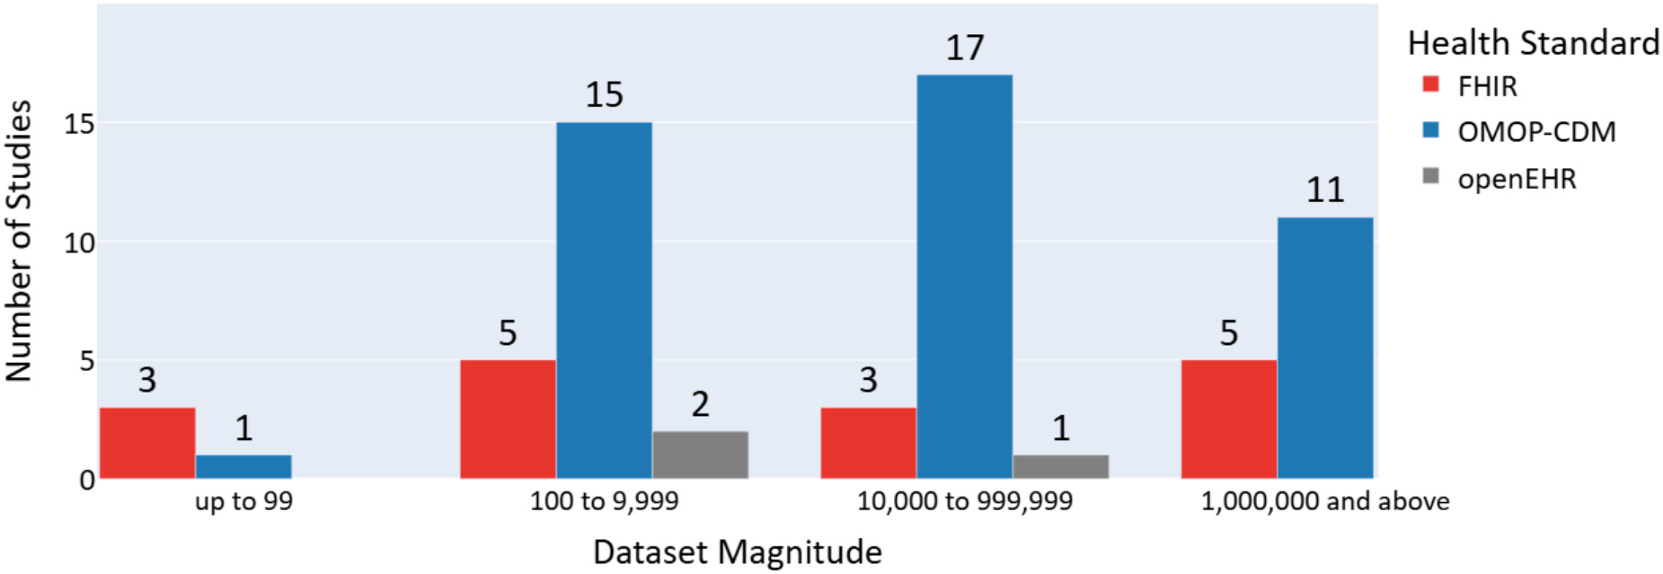
\includegraphics[width=\textwidth]{figures/paper1/fig3-dataset-magnitude.jpg}
\caption{Distribution of dataset magnitude across health data standards. Note that multiple standards might be used within the same study, meaning that counts are not mutually exclusive.}
\label{fig:paper1_dataset_magnitude}
\end{figure}

\subsubsection{How is health data standardization achieved?}
\label{sec:paper1_results_standardization}

The reviewed studies achieved health data standardization by leveraging specialized ETL tools, which aid in data cleaning, mapping, and validation. Among the 99 studies, only 15 articles \cite{bennett2023mimic,espinoza_development_2023,guo_development_2023,paris_transformation_2021,bhattacharjee_inspire_2024,almeida_bicenter-ad_2022,papez_transforming_2023,almeida_two-stage_2021,biedermann_standardizing_2021,lamer_transforming_2021,papez_transforming_2021,khalid_standardized_2021,mayer_conversion_2023,delanerolle_methodological_2022,tang_creating_2023} (15\%) provide comprehensive information about the specific ETL tools used, while 37 studies \cite{li_configurable_2022,ulgu_nationwide_2024,cai_advancing_2023,chechulina_semi-automated_2023,kempf_how_2023,yu_developing_2022,de_analyzing_2021,gruendner_framework_2021,lenert_automated_2021,li_patient-screening_2021,mishra_modified_2021,tian_application_2021,xiao_development_2021,junior_integrating_2022,raventos_transforming_2023,henke_assessing_2023,kiwuwa-muyingo_enabling_2023,kohler_eos_2023,park_cancer_2023,sinaci2023data,yu_integrating_2023,bathelt_opportunities_2022,bradshaw_garde_2022,byun_analysis_2022,bialke_fhir_2022,choi_conversion_2022,phuong_extracting_2021,tan_applying_2022,almeida_methodology_2021,baumgartner_health_2024,phelan_beyond_2024,ward_omop_2024,carus_mapping_2023,oja_transforming_2023,sathappan_transformation_2021} (37\%) provide partial information, with some tools not explicitly identified.

Studies adopting OMOP-CDM leveraged commonly used tools \cite{bhattacharjee_inspire_2024,papez_transforming_2023,almeida_methodology_2021,lamer_transforming_2021,papez_transforming_2021,khalid_standardized_2021,delanerolle_methodological_2022,rosenau_generation_2022} such as White Rabbit,USAGI, Rabbit-in-a-Hat, and ACHILLES, all developed within the OHDSI ecosystem and routinely used in OMOP-CDM implementations.

In contrast, FHIR-based conversion pipelines appear to be more diverse, involving a mix of proprietary tools (e.g., SmileCDR) \cite{ulgu_nationwide_2024,lenert_automated_2021,mishra_modified_2021,sinaci2023data,bialke_fhir_2022} and open-source solutions (e.g.,HAPI FHIR) \cite{marfoglia_towards_2025,bennett2023mimic,phelan_beyond_2024}. Lastly, openEHR implementations rely on more specialized tools, such as Clinical Knowledge Manager and openEHR EL \cite{li_configurable_2022,li_patient-screening_2021,kohler_eos_2023}.

\begin{figure}[tbp]
\centering
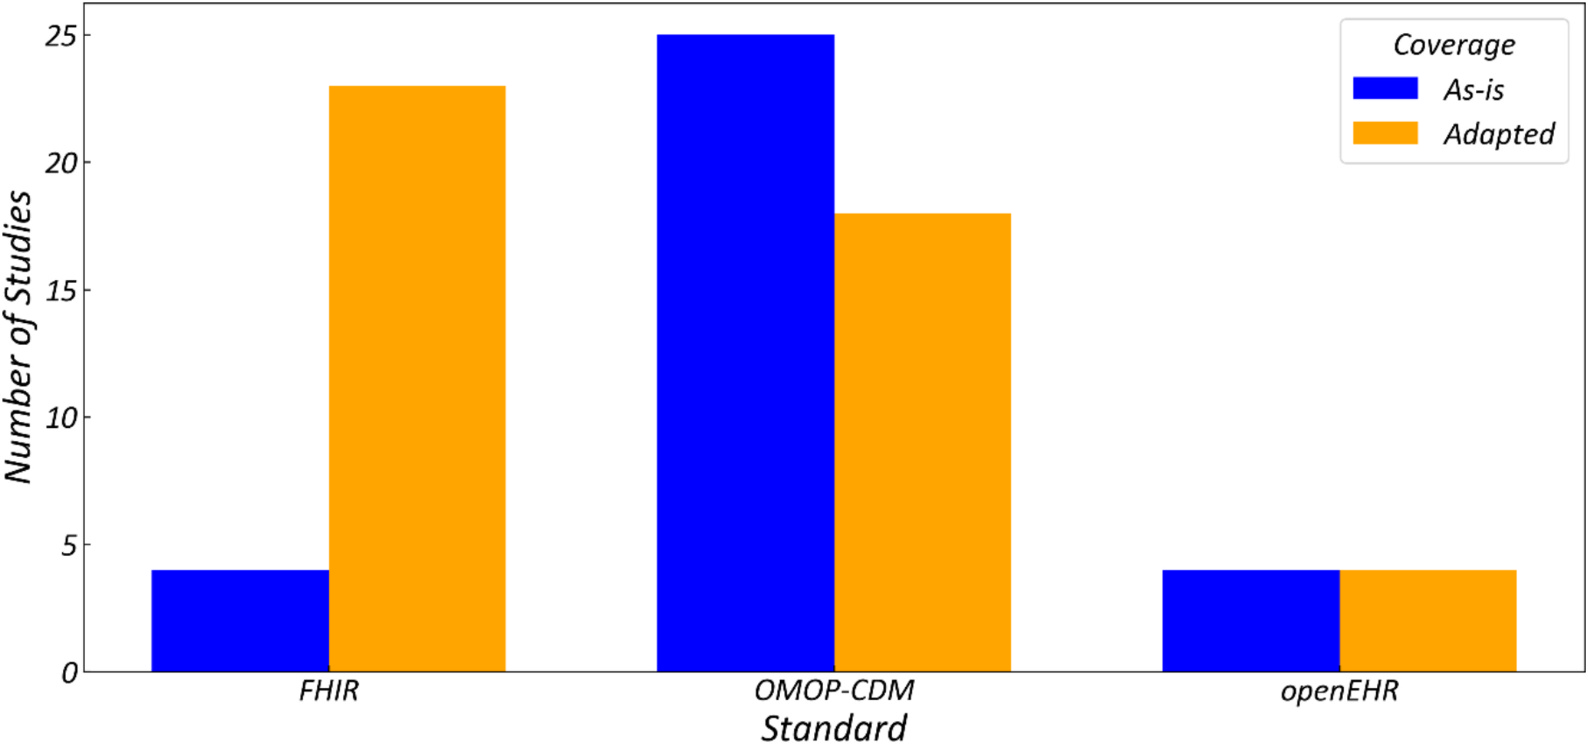
\includegraphics[width=\textwidth]{figures/paper1/fig4-coverage.jpg}
\caption{Coverage of health data standards: number of studies that used the standard as-is or adapted it.}
\label{fig:paper1_coverage}
\end{figure}

\subsubsection{How extensive is the use of standardized data in relation to the total data utilized for application implementation?}
\label{sec:paper1_results_extent}

Among the 99 studies, only 27 articles \cite{cai_advancing_2023,kempf_how_2023,jung_patient-level_2022,yu_developing_2022,kim_transforming_2021,li_patient-screening_2021,paris_transformation_2021,tian_application_2021,zong_modeling_2021,junior_integrating_2022,raventos_transforming_2023,bhattacharjee_inspire_2024,henke_assessing_2023,oliver_introducing_2023,roman-villaran_personalized_2022,almeida_methodology_2021,almeida_two-stage_2021,gulden_prototypical_2021,lamer_transforming_2021,mayer_learning_2023,kim_scalable_2023,mayer_conversion_2023,carus_mapping_2022,rosenau_generation_2022,sathappan_transformation_2021} (27\%) provided information related to the coverage of the standard (i.e., the number of variables from the original dataset mapped in the selected standard), while 77 studies \cite{bennett2023mimic,li_configurable_2022,cai_advancing_2023,chechulina_semi-automated_2023,dolin_sync_2023,espinoza_development_2023,guo_development_2023,kempf_how_2023,song_implementation_2023,bae_coronary_2022,castano_identification_2022,jung_patient-level_2022,mcguinness_extraction_2021,spotnitz_patient_2022,gomes_representation_2021,khalifa_interoperable_2021,kim_transforming_2021,li_patient-screening_2021,oliveira_openehr_2021,paris_transformation_2021,seong_fast_2021,thayer_human-centered_2021,tian_application_2021,xiao_development_2021,zong_modeling_2021,junior_integrating_2022,raventos_transforming_2023,chukwu_standardizing_2022,bhattacharjee_inspire_2024,henke_assessing_2023,kohler_eos_2023,oliver_introducing_2023,seol_effect_2023,sinaci2023data,yu_integrating_2023,bathelt_opportunities_2022,bialke_fhir_2022,choi_conversion_2022,papez_transforming_2023,phuong_extracting_2021,roman-villaran_personalized_2022,sommer_structured_2022,tan_applying_2022,almeida_methodology_2021,almeida_two-stage_2021,biedermann_standardizing_2021,gonzalez-castro_caside_2021,gulden_prototypical_2021,kawamoto_establishing_2021,kim_risk_2021,lamer_transforming_2021,mun_real-world_2021,nestsiarovich_predictors_2021,papez_transforming_2021,wesley_novel_2021,khalid_standardized_2021,wulff_transformation_2021,phelan_beyond_2024,shehab_national_2024,ward_omop_2024,carus_mapping_2023,mayer_learning_2023,kim_scalable_2023,mayer_conversion_2023,oja_transforming_2023,rinaldi_towards_2023,stellmach_creation_2023,bae_development_2022,delanerolle_methodological_2022,gruendner_architecture_2022,jung_shared_2022,rosenau_generation_2022,dolin_vcf2fhir_2021_p1,sathappan_transformation_2021,seong_incorporation_2021,sun_building_2021,tang_creating_2023} (78\%) clearly stated whether the standard was used in its original form (i.e., as-is) or if it was extended (i.e., adapted). Indeed, Fig.~\ref{fig:paper1_coverage} reports that, among these 77 studies, 27 \cite{bennett2023mimic,dolin_sync_2023,song_implementation_2023,mcguinness_extraction_2021,khalifa_interoperable_2021,seong_fast_2021,thayer_human-centered_2021,xiao_development_2021,zong_modeling_2021,chukwu_standardizing_2022,sinaci2023data,bialke_fhir_2022,roman-villaran_personalized_2022,gulden_prototypical_2021,kawamoto_establishing_2021,wesley_novel_2021,phelan_beyond_2024,shehab_national_2024,rinaldi_towards_2023,stellmach_creation_2023,bae_development_2022,gruendner_architecture_2022,jung_shared_2022,rosenau_generation_2022,dolin_vcf2fhir_2021_p1} (35\%) use FHIR, 44 \cite{cai_advancing_2023,chechulina_semi-automated_2023,guo_development_2023,kempf_how_2023,bae_coronary_2022,castano_identification_2022,jung_patient-level_2022,spotnitz_patient_2022,kim_transforming_2021,paris_transformation_2021,junior_integrating_2022,raventos_transforming_2023,bhattacharjee_inspire_2024,henke_assessing_2023,kohler_eos_2023,oliver_introducing_2023,seol_effect_2023,yu_integrating_2023,bathelt_opportunities_2022,choi_conversion_2022,papez_transforming_2023,phuong_extracting_2021,tan_applying_2022,almeida_methodology_2021,almeida_two-stage_2021,biedermann_standardizing_2021,kim_risk_2021,mun_real-world_2021,nestsiarovich_predictors_2021,papez_transforming_2021,khalid_standardized_2021,ward_omop_2024,carus_mapping_2023,mayer_learning_2023,kim_scalable_2023,mayer_conversion_2023,oja_transforming_2023,stellmach_creation_2023,delanerolle_methodological_2022,sathappan_transformation_2021,seong_incorporation_2021} (57\%) use OMOP-CDM, and 8 \cite{li_configurable_2022,gomes_representation_2021,li_patient-screening_2021,oliveira_openehr_2021,tian_application_2021,kohler_eos_2023,sommer_structured_2022,wulff_transformation_2021} (10\%) use openEHR, resulting in more than 77 studies because two papers simultaneously used two standards. Of the 27 studies involving FHIR, 23 articles \cite{bennett2023mimic,dolin_sync_2023,song_implementation_2023,khalifa_interoperable_2021,seong_fast_2021,thayer_human-centered_2021,xiao_development_2021,zong_modeling_2021,chukwu_standardizing_2022,sinaci2023data,bialke_fhir_2022,gonzalez-castro_caside_2021,gulden_prototypical_2021,kawamoto_establishing_2021,wesley_novel_2021,phelan_beyond_2024,shehab_national_2024,stellmach_creation_2023,bae_development_2022,gruendner_architecture_2022,jung_shared_2022,rosenau_generation_2022,dolin_vcf2fhir_2021_p1} (85\%) reported adapting the standard to specific use cases, often to accommodate local requirements or specialized clinical workflows. In contrast, 25 studies \cite{espinoza_development_2023,guo_development_2023,castano_identification_2022,jung_patient-level_2022,spotnitz_patient_2022,junior_integrating_2022,henke_assessing_2023,kohler_eos_2023,oliver_introducing_2023,seol_effect_2023,yu_integrating_2023,bathelt_opportunities_2022,phuong_extracting_2021,tan_applying_2022,kim_risk_2021,mun_real-world_2021,nestsiarovich_predictors_2021,khalid_standardized_2021,carus_mapping_2023,mayer_learning_2023,mayer_conversion_2023,delanerolle_methodological_2022,seong_incorporation_2021} utilizing OMOP-CDM (57\%) implemented the standard without modification, while openEHR was applied equally in both adapted \cite{gomes_representation_2021,oliveira_openehr_2021,tian_application_2021,wulff_transformation_2021} and unmodified forms \cite{li_configurable_2022,li_patient-screening_2021,kohler_eos_2023,sommer_structured_2022} (50\% each).

\subsubsection{What are the main limitations and barriers to the application of health data standards?}
\label{sec:paper1_results_limitations}

This subsection examines the key limitations of each healthcare standard based on insights gathered from the reviewed papers. Rather than addressing general challenges, we focused on issues arising from unique standards.

One of the critical barriers to OMOP-CDM adoption is its inherent complexity. The OMOP-CDM standard can be overwhelming, especially when harmonizing cohorts across different institutions.

OMOP-CDM complexity primarily stems from its data model architecture and transformation requirements. Originally designed for large-scale harmonization of heterogeneous, longitudinal EHR and administrative datasets, OMOP-CDM features an extensive relational schema with more than forty interrelated tables. The transformation of primary-care data into the OMOP structure has been shown to require complex structural mapping and extensive vocabulary alignment due to the heterogeneity of local and country-specific data sources \cite{fruchart_transforming_2024}. Evidence from comparative mapping studies indicates that the ETL phase remains the most resource-intensive aspect of OMOP adoption, demanding reconciliation of diverse terminologies and encounter representations \cite{peng_etl-process_2023,papez_transforming_2023}. Similar findings were reported for multi-country primary-care data transformations, where differences in coding systems and record granularity significantly increased implementation effort \cite{kent_common_2021}.

In contrast, FHIR employs a modular, resource-oriented architecture optimized for real-time data exchange rather than retrospective analytics, resulting in a lighter implementation burden at the interface level. openEHR, by comparison, provides a semantic modeling framework based on archetypes that ensures internal consistency but is less focused on large-scale ETL and analytic workflows.

Additionally, the OMOP-CDM structure lacks crucial clinical details, such as cognitive scores and genetic markers \cite{byun_analysis_2022}. Its patient-centric design also challenges mapping administrative and institutional data, making it less suitable for use cases requiring detailed operational insights. Another limitation is the absence of real-time data ingestion and patient re-identification mechanisms \cite{paris_transformation_2021}, restricting OMOP-CDM applicability in time-sensitive studies. Furthermore, while the OHDSI ecosystem provides robust analytical tools like ATHENA \cite{seong_incorporation_2021}, these tools demand significant computational resources, posing a barrier for institutions with limited infrastructure.

Regarding FHIR, its flexibility can be a double-edged sword \cite{xiao_development_2021,sinaci2023data,kramer_reducing_2022}. While its adaptable structure allows for personalization across different domains, this feature can lead to inconsistencies between implementations. The extension mechanism, though essential for customization, often complicates interoperability on a global scale. Another limitation is data fragmentation \cite{gonzalez-castro_caside_2021}: information is often scattered across multiple FHIR resources and extensions \cite{xiao_development_2021},making it difficult to perform efficient searches, especially without advanced server capabilities \cite{bennett2023mimic}. This latter negative aspect is also due to the lack of native support for complex multi-criteria searches \cite{gruendner_framework_2021}. Without a dedicated preprocessing module integrated into the FHIR server \cite{song_implementation_2023}, the execution of advanced queries remains cumbersome \cite{gruendner_architecture_2022}, particularly in high-volume data environments \cite{gruendner_framework_2021}. Finally, the standard follows the 80/20 rule \cite{stellmach_creation_2023} --- designed to cover 80\% of use cases while leaving the remaining 20\% to custom extensions --- which means it may not capture the full granularity of clinical data, potentially leading to data loss.

None of the authors in the studies adopting openEHR reported any limitations; therefore, no limitations have been included in this review for those studies.

\subsection{Discussion}
\label{sec:paper1_discussion}

In recent years, the adoption of health data standards has become increasingly important for achieving interoperability, facilitating clinical research, and supporting innovation in healthcare. This systematic review aimed to examine the maturity of health data standard adoption in real-world contexts, focusing on three major standards: FHIR, OMOP-CDM, and openEHR. Through the analysis of 99 selected studies, we explored the specific characteristics, applications, and limitations of these standards, as well as the broader challenges associated with their implementation. Our findings may offer a broad overview of how these standards contribute to healthcare delivery and research, highlighting both their complementary strengths and persistent barriers to widespread adoption.

Indeed, the different health data standards are not competing but complementary building blocks of a modern, interoperable health data ecosystem. Each standard plays a distinct and valuable role: openEHR to persist data, FHIR to transfer data between organizations, and OMOP-CDM to find insights into the data \cite{tsafnat_converge_2024}. The synergistic integration of these standards has shown tangible benefits across the full clinical data lifecycle. For example, Kohler et al. \cite{kohler_eos_2023} proposed a framework that integrates openEHR with OMOP-CDM. Their approach used openEHR for semantic precision and representational consistency at the care-site level and subsequently transformed openEHR archetypes into OMOP-CDM-conformant datasets, enabling standardized data reuse for research. Similarly, Peng et al. \cite{peng_etl-process_2023} developed an ETL process for harmonizing FHIR-based hospital data with OMOP-CDM. In their implementation, FHIR supported national interoperability requirements within the German Medical Informatics Initiative, while OMOP-CDM facilitated participation in international research networks such as OHDSI and DARWIN EU. Furthermore, Lenert et al. \cite{lenert_automated_2021} developed an automated approach to enable near real-time, multi-institutional data sharing for COVID-19 research. FHIR served as a canonical, real-time data exchange model compliant with U.S. interoperability regulations, while OMOP-CDM provided a harmonized analytical format suitable for research networks, including the National COVID Cohort Collaborative (N3C).

Moreover, this work underscores the critical importance of data standards in catalyzing innovation across various domains within healthcare. Among these, FHIR has emerged as a key enabler of public health applications, being featured in 14 \cite{bennett2023mimic,song_implementation_2023,de_analyzing_2021,mishra_modified_2021,xiao_development_2021,jones_real_2024,sinaci2023data,kawamoto_establishing_2021,wesley_novel_2021,phelan_beyond_2024,shehab_national_2024,peng_etl-process_2023,gruendner_architecture_2022,park_worker-centered_2021} of the 39 relevant studies (36\%). Similarly, the OMOP-CDM robust relational data model was highlighted in 26 \cite{sadsad_computable_2023,chechulina_semi-automated_2023,guo_development_2023,kempf_how_2023,bae_coronary_2022,castano_identification_2022,jung_patient-level_2022,spotnitz_patient_2022,kim_transforming_2021,wang_sociodemographic_2022,park_cancer_2023,seol_effect_2023,yu_integrating_2023,byun_analysis_2022,choi_conversion_2022,tan_applying_2022,yoo_transforming_2022,almeida_two-stage_2021,biedermann_standardizing_2021,nestsiarovich_predictors_2021,papez_transforming_2021,baumgartner_health_2024,carus_mapping_2023,carus_mapping_2022} of 55 studies (47\%) for its capacity to support complex, longitudinal analyses, reinforcing its utility in clinical research. Across the three standards examined, Clinical Medicine surfaced as the most prominent application domain, appearing in 39 \cite{sadsad_computable_2023,li_configurable_2022,ulgu_nationwide_2024,chechulina_semi-automated_2023,espinoza_development_2023,guo_development_2023,kempf_how_2023,bae_coronary_2022,castano_identification_2022,jung_patient-level_2022,mcguinness_extraction_2021,spotnitz_patient_2022,kim_transforming_2021,lenert_automated_2021,thayer_human-centered_2021,zong_modeling_2021,wang_sociodemographic_2022,chukwu_standardizing_2022,park_cancer_2023,seol_effect_2023,yu_integrating_2023,bradshaw_garde_2022,byun_analysis_2022,choi_conversion_2022,lazarova_interoperable_2022,roman-villaran_personalized_2022,sommer_structured_2022,tan_applying_2022,yoo_transforming_2022,almeida_two-stage_2021,biedermann_standardizing_2021,gonzalez-castro_caside_2021,nestsiarovich_predictors_2021,papez_transforming_2021,baumgartner_health_2024,carus_mapping_2023,rinaldi_towards_2023,carus_mapping_2022,almeida_bicenter-ad_2022} of 99 studies (39\%). This dominance likely reflects the inherently structured and protocol-driven nature of clinical workflows, which naturally lend themselves to data harmonization efforts.

FHIR modular architecture, centered on reusable resources, supports flexible system design and incremental updates \cite{park_worker-centered_2021}, enabling scalable and maintainable implementations across clinical care \cite{guinez-molinos_interoperable_2021,gulden_prototypical_2021}, public health, and research. Its strength lies in standardizing profiles and terminologies \cite{bennett2023mimic,rinaldi_towards_2023}, facilitating real-time access to complex data, including patient-reported outcomes \cite{wesley_novel_2021} and genomic information \cite{dolin_sync_2023,khalifa_interoperable_2021,seong_fast_2021,stellmach_creation_2023,dolin_vcf2fhir_2021_p1}, vital for modern clinical decision-making. FHIR is particularly well-suited to low- and middle-income countries \cite{chukwu_standardizing_2022}, where affordability and flexibility are essential. Growing adoption by major EHR vendors \cite{thayer_human-centered_2021} has further simplified its integration into existing health systems, especially in regions like Europe and the U.S. \cite{xiao_development_2021,jones_real_2024}, where supportive regulatory frameworks, including centralized IRBs \cite{eisenstein_economic_2022}, are accelerating its uptake.

OMOP-CDM stands out for its excellence in clinical decision support and secondary use of health data. Its relational model supports complex, longitudinal analyses across large datasets \cite{bhattacharjee_inspire_2024,ward_omop_2024}, making it especially valuable for clinical research and predictive and machine learning applications \cite{guo_development_2023,kim_transforming_2021,bathelt_opportunities_2022,nestsiarovich_predictors_2021}. With a mature ETL ecosystem \cite{almeida_bicenter-ad_2022} and an expanding set of analytics tools \cite{raventos_transforming_2023}, OMOP-CDM is well-suited for multi-institutional data standardization workflows where real-world data (RWD) are transformed into real-world evidence (RWE) through collaborative \cite{tan_applying_2022,mun_real-world_2021,almeida_bicenter-ad_2022} and federated analyses \cite{yu_integrating_2023,carus_mapping_2023}. Moreover, its integration with ontologies like the Human Phenotype Ontology (HPO) \cite{castano_identification_2022} extends its utility to domains such phenomics \cite{castano_identification_2022,papez_transforming_2023,khalid_standardized_2021} and oncology \cite{kempf_how_2023,park_cancer_2023,seol_effect_2023,yoo_transforming_2022,carus_mapping_2022}.

openEHR provides a robust, patient-centered standard for long-term EHR data persistence and semantic interoperability. Its two-level modeling approach \cite{wulff_transformation_2021} separates a stable reference information model from adaptable, domain-specific clinical models, thus enabling seamless collaboration between IT professionals and clinicians \cite{li_configurable_2022} within their respective domains. This separation reduces communication overhead and fosters clinically meaningful implementations \cite{wulff_transformation_2021}. Optimized for rich, longitudinal health records across a patient's lifetime, openEHR includes features such as record versioning, auditing, and the Archetype Query Language (AQL) \cite{oliveira_openehr_2021}. When combined with the Expression Language (EL) \cite{li_patient-screening_2021}, these tools enable efficient, expressive querying that can outperform traditional SQL-based methods for data retrieval and screening tasks. However, its adoption in academic literature remains limited: only 2 \cite{gomes_representation_2021,oliveira_openehr_2021} out of 8 studies (25\%) referenced its use in EHR design.

Despite the significant potential of these health data standards, several limitations persist, particularly in their ETL workflow implementation. A key observation from the reviewed studies is the inconsistent reporting of ETL tools. This lack of detail limits reproducibility and highlights a gap in the standardization of implementation processes. One of the most technically and conceptually demanding components of ETL is data mapping. This process extends well beyond structural alignment and requires interpretive judgment, contextual understanding, and domain-specific expertise. Determining whether a source variable fully corresponds to a target concept might often lead to ambiguity, particularly when integrating data collected across heterogeneous clinical settings. Mapping decisions can vary between experts, driven by differences in disciplinary background, assumptions, and local priorities, hence making data mapping an inherently subjective and resource-intensive process.

These challenges are particularly pronounced in standards such as FHIR, whose flexible and abstract resource definitions allow for multiple valid representations of the same real-world concept. While this flexibility supports extensibility and innovation, it complicates standardization and validation. The lack of external reference mappings or ``gold standards'' further exacerbates this issue. Establishing authoritative mappings would require sustained verification efforts by standard developers or regulatory bodies, which are rarely feasible in practice. Consequently, practical tools, guidelines, and consensus-driven processes within the relevant reference community become essential.

FHIR-based ETL workflows remain heterogeneous as well. Reviewed studies employed a mix of proprietary tools (e.g., SmileCDR, onFHIR.io) \cite{ulgu_nationwide_2024,lenert_automated_2021,mishra_modified_2021,sinaci2023data,bialke_fhir_2022} and open-source libraries (e.g., HAPI FHIR, SMART on FHIR) \cite{marfoglia_towards_2025,bennett2023mimic,phelan_beyond_2024}, as well as Matchbox with FHIR Mapping Language for automated data transformation using Structure Maps17,23. These tools support advanced operations such as conditional updates and adapt well to evolving data requirements. Beyond the tools gathered in this systematic literature review, the broader FHIR ecosystem includes the FHIR Tools Registry for guide publication, the Firely.NET SDK \cite{noauthor_firely_net_sdk} for.NET integration, and platforms like Simplifier.net for collaboration \cite{firely_simplifier}. Moreover, industry-grade FHIR server implementations from private companies, such as IBM (IBM\textregistered{} FHIR\textregistered{} Server) and Microsoft (FHIR Server for Azure), support the deployment of scalable solutions and provide additional capabilities, such as legacy HL7 message conversion to FHIR.

In contrast, OMOP-CDM, through the efforts of the OHDSI community in delivering such tools, demonstrates a relatively mature and cohesive ETL ecosystem \cite{bhattacharjee_inspire_2024,rosenau_generation_2022}: White Rabbit performs profiling of source datasets, summarizing structures \cite{bhattacharjee_inspire_2024,papez_transforming_2023,almeida_methodology_2021,lamer_transforming_2021,papez_transforming_2021,khalid_standardized_2021,delanerolle_methodological_2022,rosenau_generation_2022}; the Rabbit-in-a-Hat application provides a GUI for designing ETL pipelines and documenting data mapping \cite{junior_integrating_2022,raventos_transforming_2023,bhattacharjee_inspire_2024,kiwuwa-muyingo_enabling_2023,papez_transforming_2023,tan_applying_2022,lamer_transforming_2021,papez_transforming_2021,khalid_standardized_2021,delanerolle_methodological_2022}; USAGI supports the semi-automated mapping of local terminologies to OMOP-CDM standardized vocabularies \cite{cai_advancing_2023,chechulina_semi-automated_2023,guo_development_2023,raventos_transforming_2023,bhattacharjee_inspire_2024,henke_assessing_2023,kiwuwa-muyingo_enabling_2023,papez_transforming_2023,almeida_methodology_2021,almeida_two-stage_2021,lamer_transforming_2021,papez_transforming_2021,khalid_standardized_2021,ward_omop_2024,carus_mapping_2023,oja_transforming_2023,delanerolle_methodological_2022,rosenau_generation_2022,sathappan_transformation_2021,sun_building_2021}; finally, tools such as the Data Quality Dashboard (DQD) and ACHILLES allow for systematic quality checks identifying anomalies and ensuring OMOP-CDM compliance \cite{kim_transforming_2021,paris_transformation_2021,bhattacharjee_inspire_2024,papez_transforming_2023,almeida_methodology_2021,biedermann_standardizing_2021,lamer_transforming_2021,papez_transforming_2021,khalid_standardized_2021,oja_transforming_2023}.

Similarly, ETL processes involving openEHR are constrained by the technical complexity of its dual-model architecture and the limited availability of standardized tooling \cite{wulff_transformation_2021}. Only 8 studies in our review addressed openEHR ETL processes, with Clinical Knowledge Manager \cite{li_configurable_2022,kohler_eos_2023} and the openEHR Expression Language \cite{li_patient-screening_2021} being the only tools explicitly cited. Nonetheless, the ecosystem includes foundational development tools such as the ADL Workbench \cite{tian_application_2021}, Archetype Editor, EHR Server, and the opener-rm-core Java library for Reference Model integration \cite{chen_openehr_2007}.

Our findings highlight the differing natures of the selected standards. Studies using FHIR often adapt the standard --- typically by modifying existing implementation guides --- to address local or specialty-specific needs \cite{bennett2023mimic,dolin_sync_2023,song_implementation_2023,khalifa_interoperable_2021,seong_fast_2021,thayer_human-centered_2021,xiao_development_2021,zong_modeling_2021,chukwu_standardizing_2022,sinaci2023data,bialke_fhir_2022,gonzalez-castro_caside_2021,gulden_prototypical_2021,kawamoto_establishing_2021,wesley_novel_2021,phelan_beyond_2024,shehab_national_2024,stellmach_creation_2023,bae_development_2022,gruendner_architecture_2022,jung_shared_2022,rosenau_generation_2022,dolin_vcf2fhir_2021_p1}, reflecting FHIR inherent flexibility. In contrast, the rigid table structure of OMOP-CDM discourages modification; however, 33\% of the reviewed OMOP-CDM studies \cite{cai_advancing_2023,chechulina_semi-automated_2023,kempf_how_2023,kim_transforming_2021,paris_transformation_2021,raventos_transforming_2023,bhattacharjee_inspire_2024,choi_conversion_2022,papez_transforming_2023,almeida_two-stage_2021,biedermann_standardizing_2021,lamer_transforming_2021,papez_transforming_2021,ward_omop_2024,kim_scalable_2023,oja_transforming_2023} extended the model to suit medical domains or national health initiatives. openEHR, which promotes structural reuse through archetypes, was implemented without modification in about half of the analyzed studies \cite{li_configurable_2022,li_patient-screening_2021,kohler_eos_2023,sommer_structured_2022}. Due to the limited extensibility of OMOP-CDM, in some cases the concept coverage is reported to be rather low \cite{jung_patient-level_2022,yu_developing_2022}. It is noteworthy, however, that the mapped percentage is rarely reported in the articles using FHIR and openEHR standards, so it is not possible to make a comparison of variable coverage between the standards. The difference in the coverage reporting could be due to the different aims and ``cultures'' of the standard communities. FHIR is being used largely by developers for the design of efficient data exchange and clinical decision support system apps, more directed to current and future clinical data. On the other hand, OMOP-CDM users leverage massive existing datasets to be merged in a harmonized, unique clinical study, which may explain why OMOP-CDM users are more attentive to the standardization coverage.

Despite their technical maturity and complementary roles, FHIR, OMOP-CDM, and openEHR each face distinct limitations that hinder widespread adoption in healthcare settings. A key challenge is fragmentation in implementation practices. FHIR aims to enable interoperability through standardized APIs and profiles, yet inconsistent implementation across institutions, organizational disparities, and rigid mappings often result in semantic mismatches in practice \cite{xiao_development_2021,sinaci2023data,gonzalez-castro_caside_2021,kramer_reducing_2022}. While FHIR granular structure is advantageous for selective data sharing and AI applications, its layered and complex architecture poses barriers to AI integration, necessitating significant data preprocessing and transformation \cite{williams2023standardized}. OMOP-CDM, by contrast, excels in supporting large-scale research through harmonized data models and standardized vocabularies. However, the ETL process required to convert heterogeneous clinical data into OMOP-CDM is resource-intensive and technically demanding \cite{williams2023standardized,almeida_methodology_2021}, posing challenges for smaller organizations. Additionally, data transformation may lead to loss of clinical detail --- especially in domains like rare diseases --- due to the model reliance on administrative coding systems and its research-oriented design \cite{bae_coronary_2022,kohler_eos_2023,seol_effect_2023,byun_analysis_2022,papez_transforming_2023,lamer_transforming_2021,mun_real-world_2021,papez_transforming_2021,carus_mapping_2023,mayer_conversion_2023,oja_transforming_2023}. openEHR presents a different set of challenges, primarily structural rather than technical. Its archetype-based approach offers strong semantic precision and reusability, yet adoption remains limited due to its complexity and divergence from prevailing industry practices \cite{delussu_survey_2024}. The steep learning curve, the need for specialized training, and the limited alignment with cloud-native and commercial development workflows could explain its slow uptake \cite{delussu_survey_2024}. Furthermore, a lack of vendor incentives and an immature ecosystem of mapping tools between openEHR and other standards hinder broader integration \cite{delussu_survey_2024}. Performance concerns have also been noted in some studies, with openEHR systems sometimes exhibiting lower throughput compared to proprietary alternatives \cite{kryszyn_performance_2022}.

While in this paper the term maturity is used to qualitatively evaluate the degree of practical adoption and consolidation of standards in operational environments, future work may build on these findings to develop measurable criteria for maturity assessment and cross-standard comparison. Although a wide range of quantitative tools to asses technology adoption maturity exists \cite{noauthor_paho_maturity_2022,measure_evaluation_his_toolkit,noauthor_himss_maturity,liaw_digital_2021}, the content of the included papers did not allow for their comprehensive application. Moreover, as this review focused exclusively on peer-reviewed literature, our analysis did not capture evidence from non-academic sources or market-driven implementations that often represent advanced or commercially mature deployments. This introduces an inherent bias toward research-documented initiatives and may underestimate the true level of real-world standard adoption and integration, particularly in vendor-led or proprietary contexts.

Future studies on health data standard adoption could directly operationalize the frameworks to perform formal maturity assessments and comparative evaluations across standards or implementation contexts.

This systematic review has several limitations that may affect the generalizability and comprehensiveness of its findings. First, the scope was restricted to studies published within the past four years. This decision was made to prioritize recent developments, particularly those emerging in the wake of the COVID-19 pandemic, which significantly accelerated innovation in health data infrastructure. However, this temporal restriction may have led to the exclusion of earlier yet potentially influential studies. Nonetheless, the inclusion of 99 studies suggests a substantial and growing body of contemporary research in this area. Furthermore, the review may be affected by publication bias. A substantial proportion of health data standardization work occurs within private or vendor-driven settings where implementation details are rarely disclosed due to commercial or intellectual property constraints. As this study systematically analyzed peer-reviewed scientific literature, clinically deployed and commercially maintained systems were largely outside its scope. Consequently, the findings reflect research-oriented and publicly documented implementations. This limitation likely contributes to two observed patterns: (1) the predominance of research-oriented studies (87\%) \cite{bennett2023mimic,sadsad_computable_2023,cai_advancing_2023,chechulina_semi-automated_2023,dolin_sync_2023,dolin_sync_2023,espinoza_development_2023,guo_development_2023,kempf_how_2023,bae_coronary_2022,castano_identification_2022,jung_patient-level_2022,mcguinness_extraction_2021,spotnitz_patient_2022,yu_developing_2022,gomes_representation_2021,de_analyzing_2021,khalifa_interoperable_2021,kim_transforming_2021,lenert_automated_2021,oliveira_openehr_2021,paris_transformation_2021,seong_fast_2021,tian_application_2021,xiao_development_2021,zong_modeling_2021,wang_sociodemographic_2022,junior_integrating_2022,raventos_transforming_2023,chukwu_standardizing_2022,bhattacharjee_inspire_2024,henke_assessing_2023,jones_real_2024,kiwuwa-muyingo_enabling_2023,kohler_eos_2023,oliver_introducing_2023,park_cancer_2023,seol_effect_2023,sinaci2023data,yu_integrating_2023,bathelt_opportunities_2022,byun_analysis_2022,bialke_fhir_2022,choi_conversion_2022,phuong_extracting_2021,roman-villaran_personalized_2022,sommer_structured_2022,tan_applying_2022,yoo_transforming_2022,almeida_methodology_2021,almeida_two-stage_2021,biedermann_standardizing_2021,gonzalez-castro_caside_2021,gulden_prototypical_2021,kim_risk_2021,lamer_transforming_2021,lamer_transforming_2021,mun_real-world_2021,nestsiarovich_predictors_2021,papez_transforming_2021,papez_transforming_2021,khalid_standardized_2021,wulff_transformation_2021,baumgartner_health_2024,phelan_beyond_2024,ward_omop_2024,carus_mapping_2023,mayer_learning_2023,kim_scalable_2023,mayer_conversion_2023,oja_transforming_2023,peng_etl-process_2023,rinaldi_towards_2023,rinaldi_towards_2023,carus_mapping_2022,delanerolle_methodological_2022,gruendner_architecture_2022,gruendner_architecture_2022,rosenau_generation_2022,sathappan_transformation_2021,park_worker-centered_2021,seong_incorporation_2021,sun_building_2021,eisenstein_economic_2022,tang_creating_2023,almeida_bicenter-ad_2022} and (2) the limited representation of openEHR, which, despite its conceptual prominence, appeared in relatively few studies.

Indeed, future efforts could focus on leveraging the complementary strengths of existing standards to build a cohesive and interoperable health data ecosystem. In this direction, FHIR, OMOP-CDM, and openEHR may serve as complementary building blocks for a modern, interoperable health data ecosystem. Each standard may play a distinct and valuable role:

\begin{itemize}
  \item openEHR provides the foundation for persisting rich, semantically precise clinical data.
  \item FHIR enables real-time, modular data exchange across diverse systems and supports a wide range of use cases from PROs to genomics.
  \item OMOP-CDM facilitates insight generation through scalable analytics, federated research, and standardized vocabularies.
\end{itemize}

When strategically integrated, these standards can collectively support the entire data lifecycle --- from collection and persistence to exchange and secondary use --- advancing healthcare delivery, research, and innovation.

There is growing support for such a hybrid approach: for instance, by combining the peculiarities of openEHR and FHIR \cite{smolik_comparison_2023}. Although the translation between the two mappings remains challenging, the union between the semantic richness of openEHR and the real-time data exchange enabled by FHIR could better support clinical workflows, thus enhancing interoperability in both patient care and secondary data use. From an economic perspective, future work should incorporate rigorous assessment of process efficiency and economic impact. Such an analysis can inform future policy-making strategies and quantitatively prove the positive impact that the adoption of health data standards can have in the reduction of time and costs of the healthcare system.

\subsection{Code availability}
\label{sec:paper1_code_availability}

No code was adopted in this study, apart from the supporting code scripted for data visualization made in Python 3.11. This is available from the corresponding author upon reasonable request.

\subsection*{Ethics statement}

This study is a systematic review and did not involve any original research with human participants or animals. Therefore, ethical approval and informed consent were not required. The review was conducted in accordance with established methodological guidelines and the ethical standards for research synthesis. The review protocol was registered in PROSPERO (registration number: CRD42024623398).

\subsection*{Declaration of Generative AI and AI-assisted technologies in the writing process}

During the preparation of this work, the author(s) used ChatGPT model 4.0 in order to proofread some sentences in the manuscript. After using this tool/service, the author(s) reviewed and edited the content as needed and take(s) full responsibility for the content of the publication.

\subsection*{CRediT authorship contribution statement}

\textbf{Alberto Marfoglia:} Writing -- review \& editing, Writing -- original draft, Visualization, Validation, Software, Methodology, Investigation, Formal analysis, Data curation, Conceptualization. \textbf{Valerio Antonio Arcobelli:} Writing -- review \& editing, Writing -- original draft, Visualization, Validation, Software, Methodology, Investigation, Formal analysis, Data curation, Conceptualization. \textbf{Serena Moscato:} Writing -- review \& editing, Writing -- original draft, Visualization, Validation, Software, Methodology, Investigation, Formal analysis, Data curation, Conceptualization. \textbf{Antonino Amedeo La Mattina:} Writing -- review \& editing, Writing -- original draft, Methodology, Investigation, Formal analysis, Data curation, Conceptualization. \textbf{Sabato Mellone:} Writing -- review \& editing, Supervision, Project administration, Methodology, Investigation, Funding acquisition, Data curation, Conceptualization. \textbf{Antonella Carbonaro:} Writing -- review \& editing, Supervision, Project administration, Methodology, Investigation, Funding acquisition, Data curation, Conceptualization.

\subsection*{Declaration of competing interest}

The authors does not report any financial interests/personal relationships which may be considered as potential competing interests. Antonino Amedeo La Mattina is supported by the Ministry of Health.

\subsection*{Acknowledgements}

This research was funded by the Complementary National Plan PNC-I.1 ``Research initiatives for innovative technologies and pathways in the health and welfare sector'' D.D. 931 of 06/06/2022, DARE -- DigitAl lifelong pRevEntion initiative, code PNC0000002, CUP: (B53C22006450001). Authors express their gratitude to all the AlmaHealthDB Team. We used ChatGPT for assistance with parts of the English proofing.

\subsection*{Appendix A. Supplementary data}

Supplementary data to this article can be found online at \url{https://doi.org/10.1016/j.jbi.2026.105022}.

\subsection*{Data availability}

The corresponding author had full access to all data in the study and final responsibility for the decision to submit the report for publication. The data used and analyzed during the current study are available from the corresponding author upon reasonable request.

% layout: keep this paper's floats within its section
\FloatBarrier


% ============================================================================
% Paper 2 -- integrated from papers/_Computers_in_Biology_and_Medicine__FHIR_driven_Transformation_Pipeline/
% elsarticle-template-num.tex (front matter below transcribed from the elsarticle \title/\author/\affiliation,
% abstract, graphical abstract, highlights and keyword environments; body converted mechanically, see the
% integration report).
% ============================================================================
\section{Towards Real-World Clinical Data Standardization: A Modular FHIR-driven Transformation Pipeline to Enhance Semantic Interoperability in Healthcare}
\label{sec:paper2}

\noindent This section contains the article~\cite{marfoglia_towards_2025}.

\paragraph{Authors.}
Alberto Marfoglia\textsuperscript{a}, Filippo Nardini\textsuperscript{b}, Valerio Antonio Arcobelli\textsuperscript{c}, Serena Moscato\textsuperscript{c}, Sabato Mellone\textsuperscript{c}, Antonella Carbonaro\textsuperscript{a,*}

{\raggedright
\noindent\textsuperscript{a}Dept. of Computer Science and Engineering -- DISI, University of Bologna, Via dell'Universit\`a 50, 47521 Cesena, Italy\\
\textsuperscript{b}Dept. of Electrical, Electronic and Information Engineering ``Guglielmo Marconi'' -- DEI, University of Bologna, Viale del Risorgimento 2, 40136 Bologna, Italy\\
\textsuperscript{c}Dept. of Industrial Engineering -- DIN, University of Bologna, Viale del Risorgimento 2, 40136 Bologna, Italy\\
\textsuperscript{*}Corresponding author. E-mail address: antonella.carbonaro@unibo.it (A. Carbonaro).\\
Computers in Biology and Medicine 187 (2025) 109745. Available online 3 February 2025. 0010-4825/\textcopyright{} 2025 The Authors. Published by Elsevier Ltd. This is an open access article under the CC BY license (\url{http://creativecommons.org/licenses/by/4.0/}).
\par}

\subsection*{Abstract}

\textbf{Background}: Given the exponential increase in clinical data, which accounts for around 30\% of global data volume, effective information management has become crucial to ensuring robust interoperability. This trend is further expedited by implementing consumer-oriented Internet of Things platforms, contributing to the growth of the \$8.3 trillion healthcare industry. These advancements, combined with challenges such as heterogeneous data formats and a lack of incentives, necessitate the development of pragmatic infrastructures and tools that harness contemporary clinical standards like Fast Healthcare Interoperability Resources (FHIR).
\newline
\textbf{Objective}: This study aims to present a modular conversion pipeline employing a templating strategy for translating clinical data into the FHIR model. Emphasis is placed on utilizing a standard mapping specification like FHIR Mapping Language. This ensures essential properties such as platform independence, portability, and code reusability.\newline
\textbf{Methods}: The pipeline was developed incrementally, dividing its core functionalities into five modules: Input, Refinement, Mapping, Validation, and Export. These were subsequently validated by converting a dataset from a prosthetic fitting and rehabilitation center to demonstrate the approach's validity in a real-world data context.\newline
\textbf{Results}: A total of 1962 hospital stay records of 1006 unique patients were converted successfully to 15 distinct types of FHIR resources.
The successful conversion states the pipeline's effectiveness, additionally showcasing its capabilities for enhancing semantic interoperability and facilitating the reuse of real-world data.
\newline
\textbf{Conclusion}: Our approach emerges as a modular data conversion framework that addresses the limitations of existing solutions, making significant contributions to the creation of standardized, interoperable, and high-quality clinical datasets that serve as a foundation for further work.

\subsection*{Graphical abstract}

\begin{center}
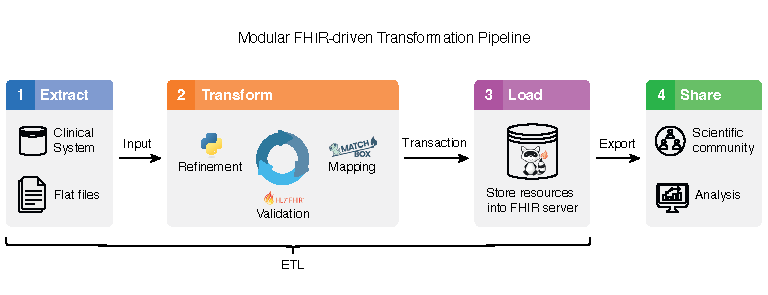
\includegraphics[width=\textwidth]{figures/paper2/grabs.pdf}
\end{center}

\subsection*{Highlights}

\begin{itemize}
\item Development of a modular conversion pipeline utilizing a templating strategy for translating clinical data into the FHIR model.
\item Emphasis on utilizing standard mapping specifications like FHIR Mapping Language for platform independence, portability, and code reusability.
\item Successful validation using a dataset from a center for prosthetic fitting and rehabilitation, confirming semantic preservation.
\item Contribution to creating standardized, interoperable, and high-quality clinical datasets through the enhancement of semantic interoperability and facilitation of real-world data reuse.
\end{itemize}

\paragraph{Keywords:} Health informatics; Standardization; Data conversion; Semantic technology; Software architecture

\subsection{Introduction}
% Please add the following required packages to your document preamble:
% \usepackage{graphicx}
% \begin{table}[t]
% %\begin{tabular}{|l|l|l|}
% \begin{tabular}{|p{0.3\linewidth}|p{0.3\linewidth}|p{0.3\linewidth}|}
% \hline
% \textbf{Problem or Issue} & \textbf{What is Already Known} & \textbf{What this Paper Adds} \\\hline
% Heterogeneous and proprietary clinical data formats hinder interoperability, complicating data reuse and undermining data semantics. & Existing solutions provide conversion pipelines butlack comprehensive, portable, and reusable mapping strategies & Presents a modular conversion pipeline utilizing templating and the FHIR Mapping Language, enhancing interoperability by providing a standardized approach for translating clinical data into the FHIR model. Addresses limitations of existing solutions, facilitating semantic preservation, platform independence, and code reusability.\\\hline
% \end{tabular}%
% \caption{Statement of significance.}
% \label{tab:statement-of-significance}
% \end{table}

% \begin{table}[ht]
% \centering
% \begin{tabular}{|l|p{0.52\linewidth}|}\hline
% \textbf{Problem or Issue} & Heterogeneous and proprietary clinical data formats hinder interoperability, complicating data reuse and undermining data semantics. \\\hline
% \textbf{What is Already Known} & Existing solutions provide conversion pipelines but lack comprehensive, portable, and reusable mapping strategies \\\hline
% \textbf{What this Paper Adds} & Presents a modular conversion pipeline utilizing templating and the FHIR Mapping Language, enhancing interoperability by providing a standardized approach for translating clinical data into the FHIR model. Addresses limitations of existing solutions, facilitating semantic preservation, platform independence, and code reusability.\\\hline
% \end{tabular}%
% \caption{Statement of significance}
% \label{tab:statement-of-significance}
% \end{table}

\begin{table}[ht]
\centering
\resizebox{\textwidth}{!}{ % Adjusts table to fit page width
\begin{tabular}{|l|p{0.9\textwidth}|} % Adjusted column widths for proper wrapping
\hline
\textbf{Problem or Issue} & Heterogeneous and proprietary clinical data formats hinder interoperability, complicating data reuse and undermining data semantics. \\
\hline
\textbf{What is Already Known} & Existing solutions provide conversion pipelines but lack comprehensive, portable, and reusable mapping strategies \\
\hline
\textbf{What this Paper Adds} & Presents a modular conversion pipeline utilizing templating and the FHIR Mapping Language, enhancing interoperability by providing a standardized approach for translating clinical data into the FHIR model. Addresses limitations of existing solutions, facilitating semantic preservation, platform independence, and code reusability. \\
\hline
\end{tabular}
}
\caption{Statement of significance}
\label{tab:paper2_statement-of-significance}
\end{table}

The healthcare landscape is marked by continuous evolution driven by advancements in medical research and technological innovation, resulting in an outstanding growth of clinical data
%CHANGED:
%NEW:
- approximately 30\% of the world’s data volume~\cite{thomason_data_2024}. This growth is further accelerated by the involvement of Big Tech companies in the USD 8.3 trillion healthcare industry. These companies have introduced consumer-focused Internet of Things (IoT) platforms and services, including Amazon Care, Apple’s wearables, and Alphabet’s artificial intelligence (AI)-driven precision medicine initiatives~\cite{thomason_data_2024}. Additionally, emerging technologies such as the IoT and 5G are transforming healthcare, with IoT expected to contribute between USD 0.5–1.8 trillion (14\%) of its total economic value by 2030~\cite{seixas-lopes_musculoskeletal_2024}. The global wearable healthcare market, valued at USD 14.4 billion in 2020, is projected to grow at an annual rate of roughly 18.9\%~\cite{thomason_data_2024}. A significant portion of this growth is driven by home healthcare, which dominated the wearable medical device market in 2021, accounting for 54.5\% of the total revenue~\cite{thomason_data_2024}.

Managing and sharing this information effectively across diverse organizations has emerged as a pivotal challenge on which the progress of the healthcare industry depends~\cite{lehne_why_2019,chatterjee_hl7_2022,kadakia_modernizing_2021}. 
To address this issue, it is essential to develop healthcare systems that are both semantically and structurally cohesive, enabling the seamless exchange of meaningful data. This necessitates the adoption of formal data descriptions, standardized vocabularies, and machine-readable formats~\cite{chatterjee_hl7_2022}. Essentially, interoperability emerges as the linchpin of the digital health revolution~\cite{lehne_why_2019,benson_why_2021}, providing a basis for efficient communication, prospective data curation, and the secondary use of real-world data in medical data science — essential elements for well-informed decision-making. Its economic potential is exemplified by the European Health Data Space (EHDS), which aims to create a unified health data ecosystem. By improving data access in healthcare and facilitating secondary use for research and innovation, the EHDS is projected to save the EU €11 billion over ten years~\cite{qeuropean}.

Despite the mandate in certain regions like the U.S. under the 21st Century Cures Act~\cite{noauthor_21st_2020} requiring the use of the Fast Healthcare Interoperability Resources (FHIR) for health data exchange, many countries lack well-defined regulatory directives and incentives. This has resulted in individual hospitals and software companies adopting custom data formats and interfaces to prioritize short-term gains, thereby hindering interoperability~\cite{benson_why_2021}. To overcome this challenge, standardization is pivotal in achieving data harmonization and improving healthcare information availability, safety, and accuracy~\cite{montazeri2023developing,lehne_why_2019}, as well as integrating heterogeneous data sources. In this context, FHIR, developed by Health Level Seven International (HL7), has emerged as a prominent standard for achieving interoperability in healthcare systems. FHIR conceptualizes healthcare data as modular resources with explicit semantics, offering flexibility and extensibility. This data standard design supports incremental adoption, promoting scalability, cost-effectiveness, and seamless integration into existing healthcare infrastructures~\cite{benson_why_2021}.
Moreover, the FHIR specification can be tailored to suit specific contexts of use through its FHIR profiles mechanism\footnote{https://build.fhir.org/profiling.html}. This feature enables the creation of customized resource definitions by applying constraints and extensions to the base resource. As a result, it promotes standardized implementations that cater to unique requirements effectively.
The recent surge in FHIR adoption can be attributed to its robust framework for exchanging electronic healthcare information and to regulatory measures implemented, particularly in countries like the U.S.~\cite{vorisek_fast_2022}.

% CHANGED:
% NEW:
Recent advancements have underscored FHIR's critical role in ensuring transparency and reproducibility in health data pipelines, particularly for AI-driven applications. Namli et al.~\cite{namli2024scalable} introduced a scalable data preparation pipeline using a declarative language to extract AI-ready datasets from EHR data while ensuring traceability and compliance with emerging regulations like the AI Act. This approach highlights the importance of transparent data transformation processes in creating reproducible AI solutions, addressing challenges such as harmonizing hierarchical FHIR data into AI-compatible formats and handling missing or irregularly sampled clinical data.

% CHANGED:
% NEW:
Emerging applications highlight FHIR's adaptability in tackling healthcare interoperability challenges. For example, platforms integrating Internet of Medical Things (IoMT) devices with 5G network slicing use FHIR to manage data heterogeneity and enable real-time data exchange~\cite{mavrogiorgou_internet_2019}. A scoping review also emphasizes FHIR's expanding role in chronic disease management, including cancer, cardiovascular diseases, and diabetes, within digital health ecosystems~\cite{gazzarata_hl7_2024}. Additionally, FHIR supports modular healthcare platforms that integrate diverse data sources to create standardized Digital Twins (DTs) of patients. These DTs provide semantic-rich foundations for advanced healthcare applications, ensuring data integrity while advancing patient-centric care~\cite{10.3389/fdgth.2023.1322428_carbonaro_connected}.
%
%
% Unfortunately, the lack of well-defined regulatory directives and incentives has resulted in the pervasive adoption of customized data formats and interfaces, primarily motivated by immediate benefits, thereby obstructing interoperability \cite{benson_why_2021}. To overcome this challenge, standardization is pivotal in achieving data harmonization and improving healthcare information availability, safety, and accuracy \cite{montazeri_developing_2023, lehne_why_2019}, as well as integrating heterogeneous data sources. In this context, the Fast Healthcare Interoperability Resources (FHIR), developed by Health Level Seven International (HL7), has emerged as a prominent and widely adopted standard for achieving interoperability in healthcare systems. FHIR conceptualizes healthcare data as modular resources with explicit semantics, offering flexibility and extensibility. This data standard design supports incremental adoption, promoting scalability, cost-effectiveness, and seamless integration into existing healthcare infrastructures \cite{benson_why_2021}. FHIR is the de facto standard for healthcare interoperability, providing a robust framework for representing and exchanging electronic healthcare information.

Nowadays, the focus of most FHIR projects is on developing FHIR-based data infrastructure and pipelines designed to provide standardized data for easy sharing and clinical analysis \cite{duda_hl7_2022}. The key features of these platforms should prioritize incorporating tools facilitating semi-automated data integration and anonymization \cite{gehrmann_what_2023}. Despite progress in this direction \cite{williams2023standardized,xiao_fhir-ontop-omop_2022,kiourtis_structurally_2019,lichtner_representation_2023}, existing solutions face limitations, particularly in terms of portability, code reuse, and maintenance.  

Bennet et al.~\cite{bennett2023mimic} converted the MIMIC-IV database into the FHIR data model to create a real-world FHIR store, an invaluable asset for research. However, the absence of a data sanitization phase and the use of internal mapping logic make the workflow challenging to share. Montazeri et al.~\cite{montazeri2023developing} developed a minimum Data Set customized for Computerized Physician Order Entry (CPOE) in the cardiovascular field, integrated with the Electronic Health Record (EHR) system through the classification and mapping of data elements into FHIR. A notable constraint is the absence of digital tools for the mapping process, necessitating individual and manual verification of each resource. Sinaci et al.~\cite{sinaci2023data} defined and implemented a methodology to enable the FAIR-ification of real-world health data, allowing domain experts to transform existing health data into FHIR via user-friendly GUIs. However, the dependence on an internal mapping language and adopting FHIR profiles, which enforce constraints on resource data fields, impede widespread adoption. Furthermore, Williams et al.~\cite{williams2023standardized} developed an FHIR-based data harmonization pipeline to facilitate an AI-friendly representation of clinical data. Despite its effectiveness, the mapping process implemented in Python and the explicit representation of source database attributes make the mappings strictly dependent on low-level programming details, impeding code reuse. 
% CHANGED:
% NEW:
Ladas et al.~\cite{ladas2022openehr} converted the German Corona Consensus (GECCO) dataset, which describes COVID-19-related patient data, into FHIR to enhance accessibility. Their approach relied on a web-based tool named openEHR-to-FHIR, designed to convert data from the openEHR model into an equivalent GECCO FHIR profile. However, the tool's implementation, which relies on Java classes with regular expressions, limits its reusability for other use cases.
Similarly, Soares et al.~\cite{soares2023omop} developed the OMOP-to-Bulk FHIR tool to process data from an EHR stored in the OMOP Common Data Model (CDM) into FHIR resources. Their workflow involved custom SQL queries to extract data into an intermediate format, which was then transformed into FHIR resources using translation rules. This process was powered by the Whistle Engine, a tool developed by Google that supports FHIR-specific functions and transformations. While effective within the OMOP framework, this solution's dependence on the OMOP CDM as the input data model greatly limits its broader adoption.
Finally, Simon et al.~\cite{simon2024metadata} explored the use of a metadata repository (MDR) to streamline the conversion of data from primary clinical systems into standardized formats. Their methodology involved extracting metadata from hospital forms, defining mappings and transformations in the MDR, and using a REST API to automate the conversion process. Despite its potential, the approach depends heavily on custom scripts, which may hinder generalizability and demand significant effort to adapt to different scenarios.


% CHANGED:
% These approaches reveal challenges arising from manual conversion and validation processes
% NEW:
These approaches, summarized in Table~\ref{tab:paper2_summary}, reveal challenges arising from manual conversion and validation processes and the use of internal mapping languages that hinder the sharing and publishing of mappings. We recognized these shortcomings and defined the essential functionalities necessary for an effective conversion pipeline. These features, detailed in Section \ref{sec:paper2_methods}, guided the development of our solution — a modular framework designed to translate data from various source formats into FHIR seamlessly.

Our approach employs a templating conversion strategy, implemented through the FHIR Mapping Language. This approach enables the definition of mappings in a standardized and declarative manner, empowering users without technical expertise to concentrate only on the data model, and avoiding low-level programming issues. Moreover, our mappings, based on a standard language definition, are language-agnostic and highly portable, facilitating seamless operation on any FHIR server. 

We converted the MOTU dataset to validate our pipeline, a retrospective study evaluating safety against falls and effectiveness for balance and mobility outcomes among different prosthetic knees~\cite{arcobelli_motu_2023}. 

% CHANGED:
% NEW:
The remainder of this manuscript is organized as follows.
Section \ref{sec:paper2_methods} outlines the methodology used in our study, including the pipeline design, architecture, and implementation.
In Section \ref{sec:paper2_results}, we present the results of the data conversion and validation processes.
Section \ref{sec:paper2_discussion} discusses the implications of our findings and potential avenues for future research. It also explores directions for further investigation.
Finally, Section \ref{sec:paper2_conclusion} summarizes the key contributions and provides concluding remarks.


\begin{table}[p]
    \centering
    \resizebox{\textwidth}{!}{ % Adjusts table to fit page width
    \begin{tabular}{|c|p{4cm}|p{4.5cm}|p{4.5cm}|} % Adjust column widths as needed
        \hline
        \textbf{Ref.} & \textbf{Goal} & \textbf{Challenges} & \textbf{Our Approach} \\
        \hline
        \cite{bennett2023mimic} & Convert the MIMIC-IV database into the FHIR data model for a real-world FHIR store & Lack of data sanitization, Internal mapping logic & Elimination of internal mapping logic, standardized and shareable mapping process \\
        \hline
        \cite{montazeri2023developing} & Develop a minimum Data Set for CPOE in the cardiovascular field, integrated with the EHR system & No digital tools for mapping, Individual manual verification required for each resource & Modular, automated mapping system eliminating manual verification \\
        \hline
        \cite{sinaci2023data} & Enable the FAIR-ification of health data using user-friendly GUIs & Dependence on internal mapping language, Enforcing of FHIR Profiles & Language-agnostic, templated approach for defining mappings \\
        \hline
        \cite{williams2023standardized} & Develop an FHIR-based data harmonization pipeline for AI-friendly clinical data representation & Mapping process dependent on Python and explicit source database attributes, limiting code reuse & Portable, reusable framework using standardized mapping language \\
        \hline
        \cite{ladas2022openehr} & Convert COVID-19-related patient data (GECCO) from the openEHR model to FHIR profiles & Implementation based on Java classes and regular expressions, limiting reusability & Reusable, standardized mapping language avoiding reliance on specific implementations \\
        \hline
        \cite{soares2023omop} & Transform EHR data stored in OMOP CDM into FHIR resources & Dependence on the OMOP CDM as the input model, limiting adoption & Flexible framework supporting multiple input models for broader applicability \\
        \hline
        \cite{simon2024metadata} & Automate the conversion of clinical data into standardized formats using an MDR & Reliance on custom scripts, requiring additional effort for generalization and maintenance & Standardized mapping language minimizing reliance on custom scripts \\
        \hline
    \end{tabular}
    }
    \caption{Summary of Related Work: The table outlines the goals and challenges of prior works in the field, highlighting their limitations and how our approach overcomes these gaps to offer novel contributions.}
    \label{tab:paper2_summary}
\end{table}


% \begin{table}[ht]
%     \begin{tabularx}{\textwidth}{|c|l|l|l|}
%         \hline
%          \textbf{Ref.} & \textbf{Goal} & \textbf{Challenges} & \textbf{Our Approach}
%          \\\hline
%          \cite{bennett_mimic-iv_2023} & Convert the MIMIC-IV database into the FHIR data model for a real-world FHIR store & Lack of data sanitization, Internal mapping logic & Elimination of internal mapping logic, standardized and shareable mapping process
%          \\\hline
%          \cite{montazeri_developing_2023} & Develop a minimum Data Set for CPOE in the cardiovascular field, integrated with the EHR system & No digital tools for mapping, Individual manual verification required for each resource & Modular, automated mapping system eliminating manual verification
%          \\\hline
%          \cite{sinaci_data_2023} & Enable the FAIR-ification of health data using user-friendly GUIs & Dependence on internal mapping language, Enforcing of FHIR Profiles & Language-agnostic, templated approach for defining mappings
%          \\\hline
%          \cite{williams_standardized_2023} & Develop an FHIR-based data harmonization pipeline for AI-friendly clinical data representation & Mapping process dependent on Python and explicit source database attributes, limiting code reuse & Portable, reusable framework using standardized mapping language
%          \\\hline
%          \cite{ladas_2022} & Convert COVID-19-related patient data (GECCO) from the openEHR model to FHIR profiles & Implementation based on Java classes and regular expressions, limiting reusability & Reusable, standardized mapping language avoiding reliance on specific implementations 
%          \\\hline
%          \cite{soares_2023} & Transform EHR data stored in OMOP CDM into FHIR resources & Dependence on the OMOP CDM as the input model, limiting adoption & Flexible framework supporting multiple input models for broader applicability
%          \\\hline
%          \cite{simon_2024} & Automate the conversion of clinical data into standardized formats using an MDR & Reliance on custom scripts, requiring additional effort for generalization and maintenance & Standardized mapping language minimizing reliance on custom scripts
%          \\\hline
%     \end{tabularx}
%     \caption{Summary of Related Work and advancements of the proposed solution.}
%     \label{tab:summary}
% \end{table}


% \begin{table}[h]
%     \begin{tabularx}{\textwidth}{|c|X|X|X|}
%         \hline
%          \textbf{Ref.} & \textbf{Focus} & \textbf{Limitations} & \textbf{Our Contribution}
%          \\\hline
%          \cite{bennett_mimic-iv_2023} & Converted MIMIC-IV in FHIR & Absence of data sanitization, Internal mapping logic & Explicit data preprocessing phase, FHIR Mapping Language
%          \\\hline
%          \cite{montazeri_developing_2023} & Developed a dataset for the CPOE in the cardiovascular field & Individual and manual verification of resources & FHIR Server performs validation of produced resources
%          % verifica manuale delle risorse prodotte
%          \\\hline
%          \cite{sinaci_data_2023} & User-friendly GUIs to assist the transformation of health data into FHIR & Internal mapping language, Enforcing of FHIR Profiles & FHIR Mapping Language
%          % internal mapping language, custom profiles
%          \\\hline
%          \cite{williams_standardized_2023} & Data harmonization pipeline to create AI-friendly representation of health data & dependency on technical implementation details, hard to reuse code & FHIR Mapping Language, reusable pipeline
%          % extremely dependent on specific fields + Python + hard to reuse code
%          \\\hline
%     \end{tabularx}
%     \caption{Summary of related works and advancements of the proposed experiment.}
%     \label{tab:summary}
% \end{table}

% The detailed abbreviations and definitions used in the paper are listed in Table \ref{tab:abbreviations}.

% \begin{table}[t]
% \begin{tabular}{|l|l|}
% \hline
% \textbf{Abbreviation} & \textbf{Definition} \\\hline
% ATC & Anatomical Therapeutic Chemical) \\\hline
% CPOE & Physician Order Entry \\\hline
% EHR & Electronic Health Record \\\hline
% ETL & Extract Transform Load \\\hline
% FAIR & Findable, Accessible, Interoperable, and Reusable \\\hline
% FHIR & Fast Healthcare Interoperability Resources \\\hline
% GUI & Graphical User Interface \\\hline
% HAPI FHIR & Java implementation of the HL7 FHIR standard \\\hline
% HL7 & Health Level Seven International \\\hline
% JPA & Java Persistence API \\\hline
% MIMIC & Multi-parameter Intelligent Monitoring for Intensive Care \\\hline
% NLP & Natural Language Processing \\\hline
% RDF & Resource Description Framework \\\hline
% UOM & Units of Measurement \\\hline
% \end{tabular}%
% \caption{List of abbreviations and acronyms used in the paper.}
% \label{tab:abbreviations}
% \end{table}

\subsection{Methods}\label{sec:paper2_methods}
Our work focuses on establishing a conversion pipeline that seamlessly translates data from diverse source formats into modern clinical standards, thereby enhancing healthcare interoperability. This section delineates the development strategy, the architectural framework, the implementation methodologies, and the tools employed in crafting the pipeline. 

\subsubsection{Pipeline design}

\paragraph{Templating Strategy for Declarative Mapping}
Our conversion process relies on a templating strategy that articulates data mappings in a declarative manner. This approach decouples mapping definitions from a specific programming language, promoting flexibility and adaptability across various data models and formats. 

\paragraph{Modular Architecture for Structural Advantages}
The conversion pipeline is structured into modular components, providing several architectural advantages crucial for robustness and scalability: 

\begin{itemize}
    \item \textbf{Maintainability}: The modular design prevents unwanted dependencies between components. This isolation ensures that any requirements alterations impact only the relevant module, minimizing unintended consequences.
    \item \textbf{Incremental Development}: Breaking tasks into distinct components allows for an incremental implementation workflow. This "divide and conquer" approach facilitates a more manageable and systematic development process. 
    \item \textbf{Reusability}: These modular components are designed for reuse across various pipeline implementations. This feature significantly reduces the time needed to address new use cases.
    \item \textbf{Testing and Debugging}: The well-defined responsibilities of each module enable precise control over the software. This granularity simplifies the testing and debugging of smaller, individual components, streamlining the development, and troubleshooting process. 
\end{itemize}

\subsubsection{Pipeline architecture}

The design and development of our pipeline are based on the Extract Transform Load (ETL) framework~\cite{denney_validating_2016}, and its functionalities were organized into sequential modules (Figure~\ref{paper2_1-pipeline-architecture}).  
\begin{enumerate}
    \item \textit{Input}: This module represents the strategy to acquire input data from a specific source, with no restrictions on the input data model and format, as long as a proper API to gather data is provided (e.g., databases, platforms with HTTP API, files, etc.). Additionally, this module addresses data security and regulatory compliance, ensuring that data quality, integrity, and confidentiality are not compromised. 
    \item \textit{Refinement}: This module is designed to preprocess and refine input data. Given the diverse formats and varying quality of the source datasets, this module ensures a uniform output. Moreover, it ensures consistency by eliminating missing data and structuring the information (e.g. using JSON format) to enable seamless conversion operations in subsequent steps. Specifically, the module preserves rows with non-essential null values and removes the ones where missing data are crucial for conveying the meaning of the information.
    \item \textit{Mapping}: This module takes the sanitized source data as input and performs the conversion to the target data model by employing a templating strategy. 
    \item \textit{Validation}: It carries out all the procedures aimed at checking the conformity of output resources with the standard target data model. In case of undesirable outcomes, the module takes immediate action to notify the presence of invalid data. It also initiates any roll-back functions to maintain the integrity of the system's state. 
    \item \textit{Publishing}: The final module executes the necessary logic to store the information in an accessible repository. It also provides essential functionalities, such as querying, exporting, and logging, which enable developers to debug results and design automated tests.
\end{enumerate}

\begin{figure}[ht]
\centerline{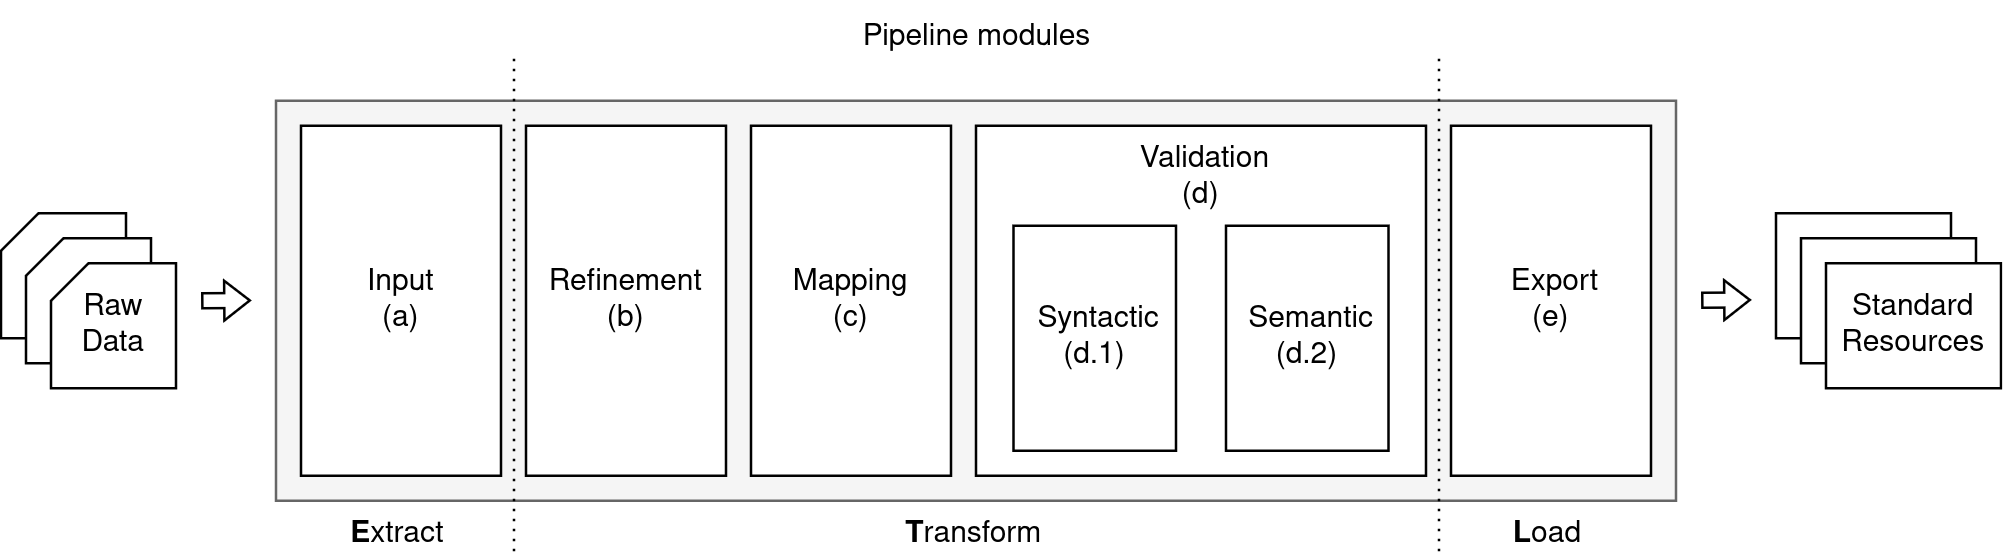
\includegraphics[width=\textwidth]{figures/paper2/1-pipeline-architecture.png}}
\caption{Modules representation of the pipeline architecture, organized according to the Extract, Transform, and Load (ETL) process steps.}
\label{paper2_1-pipeline-architecture}
\end{figure}

\subsubsection{Pipeline implementation}
% CHANGED:
% Our pipeline was methodically constructed in stages, employing data extracted from a relational database and adhering to the HL7 FHIR standard for the output data model. The choice of HL7 FHIR was driven by its flexibility, scalability, and ability to integrate with modern healthcare systems seamlessly, ensuring compatibility and interoperability across diverse data formats and systems in the healthcare domain.
% NEW:
Our pipeline was methodically constructed in stages, employing data extracted from a database and compliant with the HL7 FHIR standard for the output data model. The choice of HL7 FHIR was driven by its flexibility, scalability, and ability to integrate with modern healthcare systems seamlessly, ensuring compatibility and interoperability across diverse data formats and systems in the healthcare domain.

% CHANGED:
% The \textit{Input} (a) and \textit{Refinement} (b) modules (Figure \ref{2-pipeline-implementation}) were implemented using Python scripts supported by data manipulation libraries. These scripts transform the source relational data into sanitized JSON documents for further processing. In our specific case, the developed modules do not include any security checks because the dataset to be converted was already anonymized and verified for quality and integrity at the source.
% NEW: 
The \textit{Input} (a) and \textit{Refinement} (b) modules (Figure \ref{paper2_2-pipeline-implementation}) were implemented using Python scripts supported by data manipulation libraries. These scripts transform the source data into sanitized JSON documents for further processing. In our specific case, the developed modules do not include any security checks because the dataset to be converted was already anonymized and verified for quality and integrity at the source.

The \textit{Mapping} (c) module was developed utilizing Matchbox, a versatile FHIR templating engine characterized by its offline transformation capabilities, allowing standalone microservice deployment, and providing seamless integration as a Java library. Matchbox transforms input JSON object into an FHIR Transaction\footnote{https://build.fhir.org/http.html\#transaction}, a mechanism that empowers clients to send multiple interactions to a server to be processed atomically. This approach adopts the FHIR Bundle Resource as the transport, serving as a container for a collection of FHIR resources. The transactional approach has proved invaluable to performing non-trivial operations, such as storing a collection of related resources, performing conditional creates or updates on existing ones, etc. These features ensure the flexibility of our pipeline to accommodate future evolutions and changing requirements. Matchbox leverages templates defined using the FHIR Mapping Language\footnote{https://build.fhir.org/mapping-language.html} to efficiently transform data from any format to the FHIR data model. Specifically, these templates are parsed into Structure Maps, a detailed set of rules describing the relationships between different data structures, required to enable their automatic conversion. Both the incoming data structures and the resulting FHIR resources are represented by instances of Structure Definition – an FHIR resource that serves as a metamodel for describing schemas. To ensure the integrity of the process, Matchbox conducts syntactic validation (d.1) of the results using the built-in Structure Definitions of the FHIR data model. This step adds a quality control layer, aimed at verifying adherence of produced results with the FHIR specification. 

Upon completion of the pipeline, the HAPI FHIR JPA Server\footnote{https://hapifhir.io/}, an open-source, self-contained solution, was deployed. This server implements storage and retrieval logic without additional coding and exposes a RESTful API. Its primary role involves semantic validation (d.2) of incoming resources concerning the official HL7 Structure Definitions before storing them in the database (e). Lastly, data from the server can be exported in various file formats such as XML, JSON, and FHIR-RDF.

\begin{figure}
\centerline{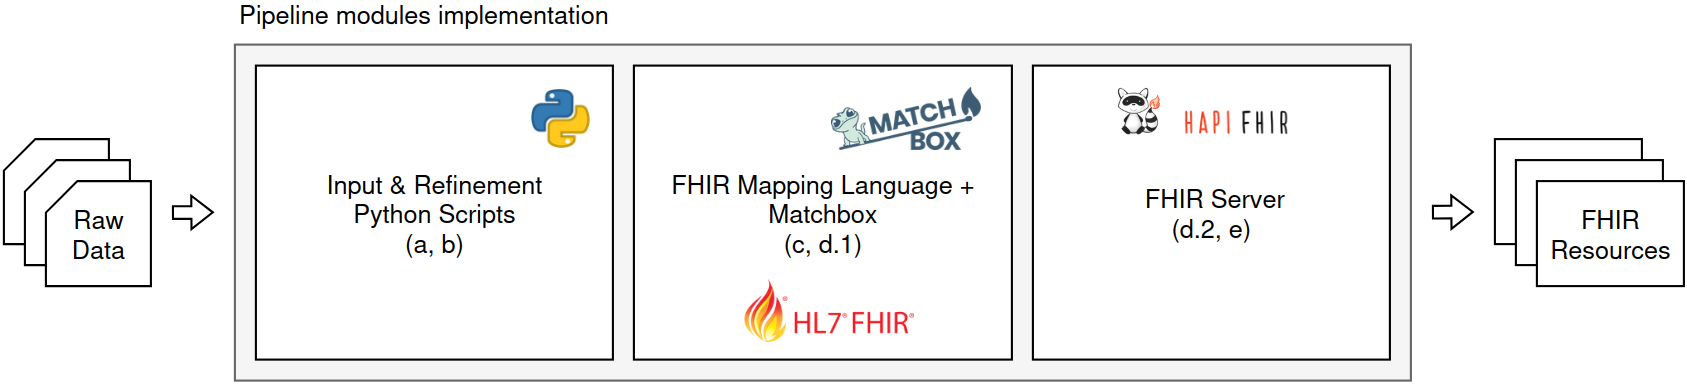
\includegraphics[width=\textwidth]{figures/paper2/2-pipeline-implementation.png}}
\caption{A possible implementation of the pipeline. The identifiers (a, b), (c, d.1), and (d.2, e) refer to the modules of the pipeline architecture shown in Figure \ref{paper2_1-pipeline-architecture}.}
\label{paper2_2-pipeline-implementation}
\end{figure}

\subsubsection{Validation Methodology}
To rigorously assess the accuracy of our pipeline, we focused on converting the MOTU dataset to the FHIR model. MOTU originates from a retrospective observational study conducted at the Italian National Institute for on-the-Job Injuries (INAIL) Prosthesis Center in Budrio, Italy. The study was approved by the Ethics Committee “Area Vasta Emilia Centro” (ref. MOTU 18088, CE AVEC n. 380/2018/OSS/AUSLBO) and complies with the Declaration of Helsinki. It aims to evaluate safety against falls and effectiveness for balance and mobility outcomes among prosthetic knees. The dataset is provided in Comma Separated Values (CSV) format and composed of 1962 hospital stays of 1006 patients with unilateral trans-femoral amputation from January 2011 to May 2020. It includes five tables: Patient, HospitalStay, Fall, DrugHospitalStay, and ProstheticKnee. Patient data feature anonymous IDs, age, and gender, while HospitalStay records admission/discharge dates, amputation details, rehabilitation goals, and assessments on balance, mobility, and daily living activities through questionnaires and functional tests. The Fall table provides information about 146 falls experienced during hospitalizations, detailing prosthesis use and resulting injuries. The DrugHospitalStay table reports information about the medication intake for each hospital stay, listed by trade name and ATC (Anatomical Therapeutic Chemical) code, and counts 3035 instances. The Knee table contains 40 different prosthetic knees, characterized by device details, and manufacturer specifics. To maintain transparency and reproducibility, the input dataset used in this study is publicly available on Zenodo~\cite{arcobelli_motu_2024}. 

% \begin{figure}
% \centerline{\includegraphics[width=\textwidth]{images/4-motu-er.png}}
% \caption{ER schema representing the MOTU dataset.}
% \label{4-motu-er}
% \end{figure}

As a strategy for assessing the completeness and accuracy of the conversion outcomes, we defined five sample queries (Table \ref{tab:paper2_validation-queries}) encompassing a wide range of tables, columns, and data types within the source model. These queries were designed in collaboration with experts from the INAIL, one of Italy's largest prosthetic centers, including a researcher with 30 years of experience and a physical therapist involved in rehabilitating patients with amputations. 
First, we employed the pandas library in Python to execute the queries on the original dataset, ensuring that the logic and criteria set by the domain experts were faithfully replicated. Subsequently, using the SPARQL querying language, we developed corresponding queries replicating the logic of the original ones. This process involved retrieving the FHIR resources in FHIR/RDF format from the HAPI FHIR server's REST API and then uploading them to an Apache Jena Fuseki\footnote{https://jena.apache.org/documentation/fuseki2/} server, an easy to setup open-source SPARQL server that enables simple querying of data through a web interface. The primary goal of such an approach was to compare the resulting number of retrieved instances, aiming for identical outcomes on corresponding queries to confirm the success of the transformation. 

% CHANGED:
% NEW:
To ensure high data quality in the resulting dataset, we adopted the Kahn framework~\cite{kahn_harmonized_2016}, a systematic methodology for data quality assurance. The framework emphasizes three main categories: \textit{Conformance}, which checks the data against syntax and structural constraints; \textit{Completeness}, which ensures that there are no missing values; and \textit{Plausibility}, which assesses the believability and truthfulness of the data values. Each category is further divided into subcategories, providing a detailed structure for quality evaluation (Table~\ref{tab:paper2_kahn-indicators}).

The framework distinguishes between two evaluation contexts: verification, which assesses how well the data aligns with local knowledge and expectations, and validation, which uses external knowledge and benchmarks to evaluate quality. Our study focuses on the verification context, using the precise definitions of data quality of the Kahn framework in all categories to evaluate how effectively our methodology addresses these standards.


\begin{table*}[ht]
\resizebox{\textwidth}{!}{%
\begin{tabular}{|l|l|l|}
\hline
\textbf{Query} & \textbf{MOTU Table(s)} & \textbf{FHIR Resources} \\\hline
Q1: How many patients who came for an initial supply return for a second hospitalization? & HospitalStay & Encounter \\\hline
Q2: How many patients transition from the initial supply of a mechanical knee to a second supply of an electronic knee? & Knee & \begin{tabular}[c]{@{}l@{}}Patient \\ DeviceRequest \\ DeviceDefinition\end{tabular} \\\hline
\begin{tabular}[c]{@{}l@{}}Q3: How many patients use anxiolytics/antidepressants (ATC Code: N06A and N05A) related to the risk of falls?\end{tabular} & Drug & \begin{tabular}[c]{@{}l@{}}Patient \\ Medication \\ MedicationRequest\end{tabular} \\\hline
Q4: Hospital stays from patients over 65 years old? & \begin{tabular}[c]{@{}l@{}}Knee \\ Patient\end{tabular} & \begin{tabular}[c]{@{}l@{}}Patient \\ DeviceRequest\end{tabular} \\\hline
Q5: How many falls per type of prosthesis (AMK, FK, etc.) & \begin{tabular}[c]{@{}l@{}}HospitalStay \\ Fall \\ Knee\end{tabular} & \begin{tabular}[c]{@{}l@{}}DeviceDefinition \\ DeviceRequest \\ Encounter \\ AdverseEvent\\\end{tabular}\\\hline
\end{tabular}%
}
\caption{Demonstration queries used to validate the mapping results. It shows the MOTU tables and the corresponding FHIR resources involved in each query.}
\label{tab:paper2_validation-queries}
\end{table*}

\begin{table*}[ht]
\resizebox{\textwidth}{!}{%
\begin{tabular}{|l|p{5cm}|p{9cm}|} % Adjust column widths
\hline

\multicolumn{1}{|c|}{\textbf{DQA}} & \multicolumn{1}{c|}{\textbf{Description}}                           & \multicolumn{1}{c|}{\textbf{Implementation}}                                                                                                                                                                                                                                                  \\ \hline
Value Conformance                  & Data values conform to allowed formats and values                   & \multirow{3}{=}{Adopting an FHIR Server with strict validation features ensures that data values conform to the correct formats, relational constraints are respected, and required values are always present, thus guaranteeing completeness and data integrity.}                             \\ \cline{1-2}
Relational Conformance             & Data values conform to relational constraints and no duplicate keys &                                                                                                                                                                                                                                                                                               \\ \cline{1-2}
Completeness                       & Absence of data under a predefined threshold                        &                                                                                                                                                                                                                                                                                               \\ \hline
Computational Conformance          & Computed values conform to programming specification                & Computed values, like the number of medications, are not stored, as they can be derived dynamically using FHIRPath queries.                                                                                                                                                                   \\ \hline
Uniqueness Plausibility            & There aren’t two or more resources that identify the same subject   & By adopting FHIR transactions for incremental updates, the risk of creating duplicate resources for the same patient is eliminated.                                                                                                                                                           \\ \hline
Atemporal Plausibility             & Data measures are coherent to a local knowledge                     & \multirow{2}{=}{During the pre-processing phase, Python scripts with custom rules are used to validate input data, ensuring that data adheres to expected properties and is consistent with local knowledge.} \\ \cline{1-2}
Temporal Plausibility              & Data measures are coherent with expected temporal properties        &                                                                                                                \\ \hline
\end{tabular}%
}
\caption{Implementation strategies for the Kahn framework data quality assessments (DQA).}
\label{tab:paper2_kahn-indicators}
\end{table*}

% \begin{table}[ht]
% \begin{tabular}{|l|p{3cm}|p{6cm}|}
% \hline
% \multicolumn{1}{|c|}{\textbf{DQA}} & \multicolumn{1}{c|}{\textbf{Description}}                           & \multicolumn{1}{c|}{\textbf{Implementation}}                                                                                                                                                                                                                                                  \\ \hline
% Value Conformance                  & Data values conform to allowed formats and values                   & \multirow{3}{*}{\parbox{6cm}{Adopting an FHIR Server with strict validation features ensures that data values conform to the correct formats, relational constraints are respected, and required values are always present, thus guaranteeing completeness and data integrity.}}                             \\ \cline{1-2}
% Relational Conformance             & Data values conform to relational constraints and no duplicate keys &                                                                                                                                                                                                                                                                                               \\ \cline{1-2}
% Completeness                       & Absence of data under a predefined threshold                        &                                                                                                                                                                                                                                                                                               \\ \hline
% Computational Conformance          & Computed values conform to programming specification                & Computed values, like the number of medications, are not stored, as they can be derived dynamically using FHIRPath queries.                                                                                                                                                                   \\ \hline
% Uniqueness Plausibility            & There aren’t two or more resources that identify the same subject   & By adopting FHIR transactions for incremental updates, the risk of creating duplicate resources for the same patient is eliminated.                                                                                                                                                           \\ \hline
% Atemporal Plausibility             & Data measures are coherent to a local knowledge                     & \multirow{2}{*}{\parbox{6cm}{During the pre-processing phase, Python scripts with custom rules are used to validate input data, ensuring that data adheres to expected properties and is consistent with local knowledge.}} \\ \cline{1-2}
% Temporal Plausibility              & Data measures are coherent with expected temporal properties        &                                                                                                                                                                                                                                                                                               \\ \hline
% \end{tabular}
% \caption{Implementation strategies for the Kahn framework data quality assessments (DQA).}
% \label{tab:kahn-indicators}
% \end{table}

\subsection{Results}\label{sec:paper2_results}
\begin{figure}
\centerline{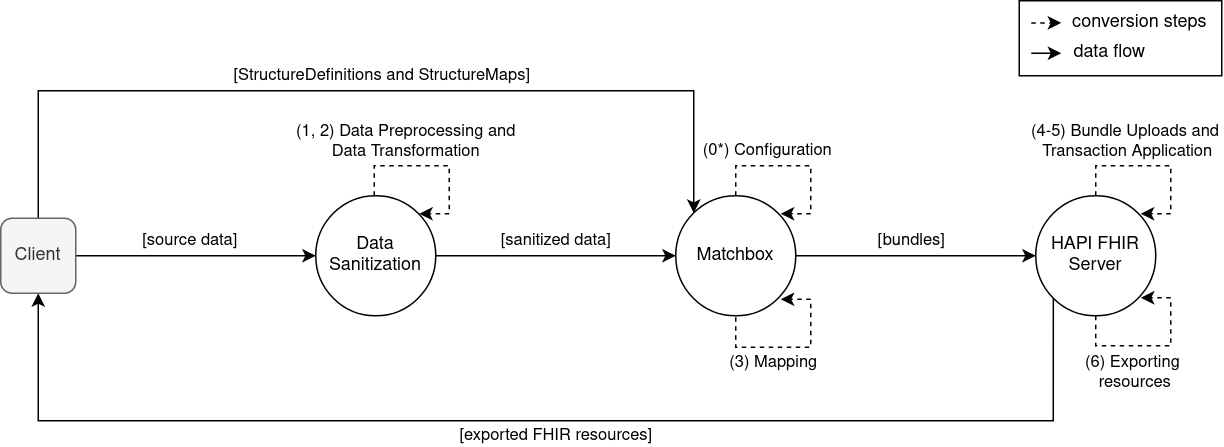
\includegraphics[width=\textwidth]{figures/paper2/3-pipeline-workflow.png}}
\caption{Representation of the role of different services participating in the pipeline. (*) The setup action is performed only once, during the initial configuration on the pipeline.}
\label{paper2_3-pipeline-worflow}
\end{figure}

The implemented pipeline successfully converted the MOTU dataset into FHIR-compliant resources~\cite{arcobelli2024fhir}. The transformation process, leveraging the previously described modules, encompassed the following key steps (Figure \ref{paper2_3-pipeline-worflow}): 

\begin{itemize}
    \item \textbf{Configuration Setup (Step 0)}: Upon deployment, the pipeline was configured by uploading Structure Definitions and Structure Maps obtained in collaboration with MOTU dataset experts~\cite{arcobelli_motu_2023}. 
    \item \textbf{Data Preprocessing (Step 1)}: Raw data from the MOTU dataset~\cite{arcobelli_motu_2024} underwent a thorough preprocessing step by using data sanitization services. This step ensured data quality, consistency, and compatibility with subsequent pipeline stages. 
    \item \textbf{Data Transformation (Step 2)}: The CSV data was transformed into JSON objects to streamline processing by Matchbox. This step included renaming, typing, and filtering source data fields. 
    \item \textbf{Mapping (Step 3)}: Matchbox transformed each JSON object into an FHIR Transaction. Moreover, Matchbox performed a syntactic validation to ensure the correctness of input and output data schemas. 
    \item \textbf{Bundles Upload (Step 4)}: Generated Bundles were dispatched individually to the HAPI FHIR server to validate and store the enclosed resources. Placeholder IDs, temporary and randomly generated UUIDs, were used to link resources within the Bundle, facilitating the determination of corresponding concepts and preventing duplications. 
    \item \textbf{Transaction Application (Step 5)}: Upon arrival at the HAPI FHIR server, Bundles underwent a processing step with reference integrity checks, resolution of temporary UUIDs, and assessment of resource conformity to FHIR profiles using the server's integrated FHIR Instance Validator module\footnote{https://hapifhir.io/hapi-fhir/docs/validation/instance\_validator.html}. This will use terminology services to validate codes, and StructureDefinitions to validate semantics. Successful transactions modified the state of the server, enabling incremental updates to the same resource from subsequent Bundles. On the other hand, failed transactions triggered a complete rollback to the previous state, ensuring successful storage only upon error-free processing. 
    \item \textbf{Exporting Resources (Step 6)}: All stored resources within the HAPI FHIR server resulting from the conversion process were exported in NDJSON format using the server's built-in FHIR Bulk Data Access protocol. This operation organized FHIR resources by their type and segmented them into files. The resulting FHIR resources dataset can be accessed on Zenodo~\cite{arcobelli_fhired_2024}.
\end{itemize}

A concrete example of data workflow conversion is illustrated in Figure \ref{paper2_5-data-conversion-workflow}. In Step 1, the initial phase entailed data sanitization, involving the removal of unused columns, and the conversion of dates into the ISO 8601 format. Afterward, in Step 2, the data is transformed into JSON format, enabling its utilization through Matchbox (Figure \ref{paper2_5-data-conversion-workflow}.b).
Step 3 encompassed the mapping of the source data onto a Bundle comprising FHIR-compliant resources, each identified by temporary UUIDs, thereby enabling seamless cross-referencing (Figure \ref{paper2_5-data-conversion-workflow}.c). Notably, the semantic richness of FHIR resources was enhanced by the integrating formal CodeSystems. Subsequently, the Bundle was transmitted to the HAPI FHIR server to execute the necessary transaction (Step 4). Finally, in Step 5, the resultant FHIR resources were individually stored in the HAPI FHIR server, and their temporary UUIDs were substituted with universal ones to enable their integration with the existing knowledge (Figure \ref{paper2_5-data-conversion-workflow}.d).

% CHANGED:
% NEW:
The experiment was conducted on a system with an Intel Core i9-14900KF processor (32 cores) and 128 GB of RAM, running Ubuntu 24.04.1 LTS. The pipeline converted the entire MOTU dataset in 8 minutes and 52.467 seconds.

\begin{figure}
\centerline{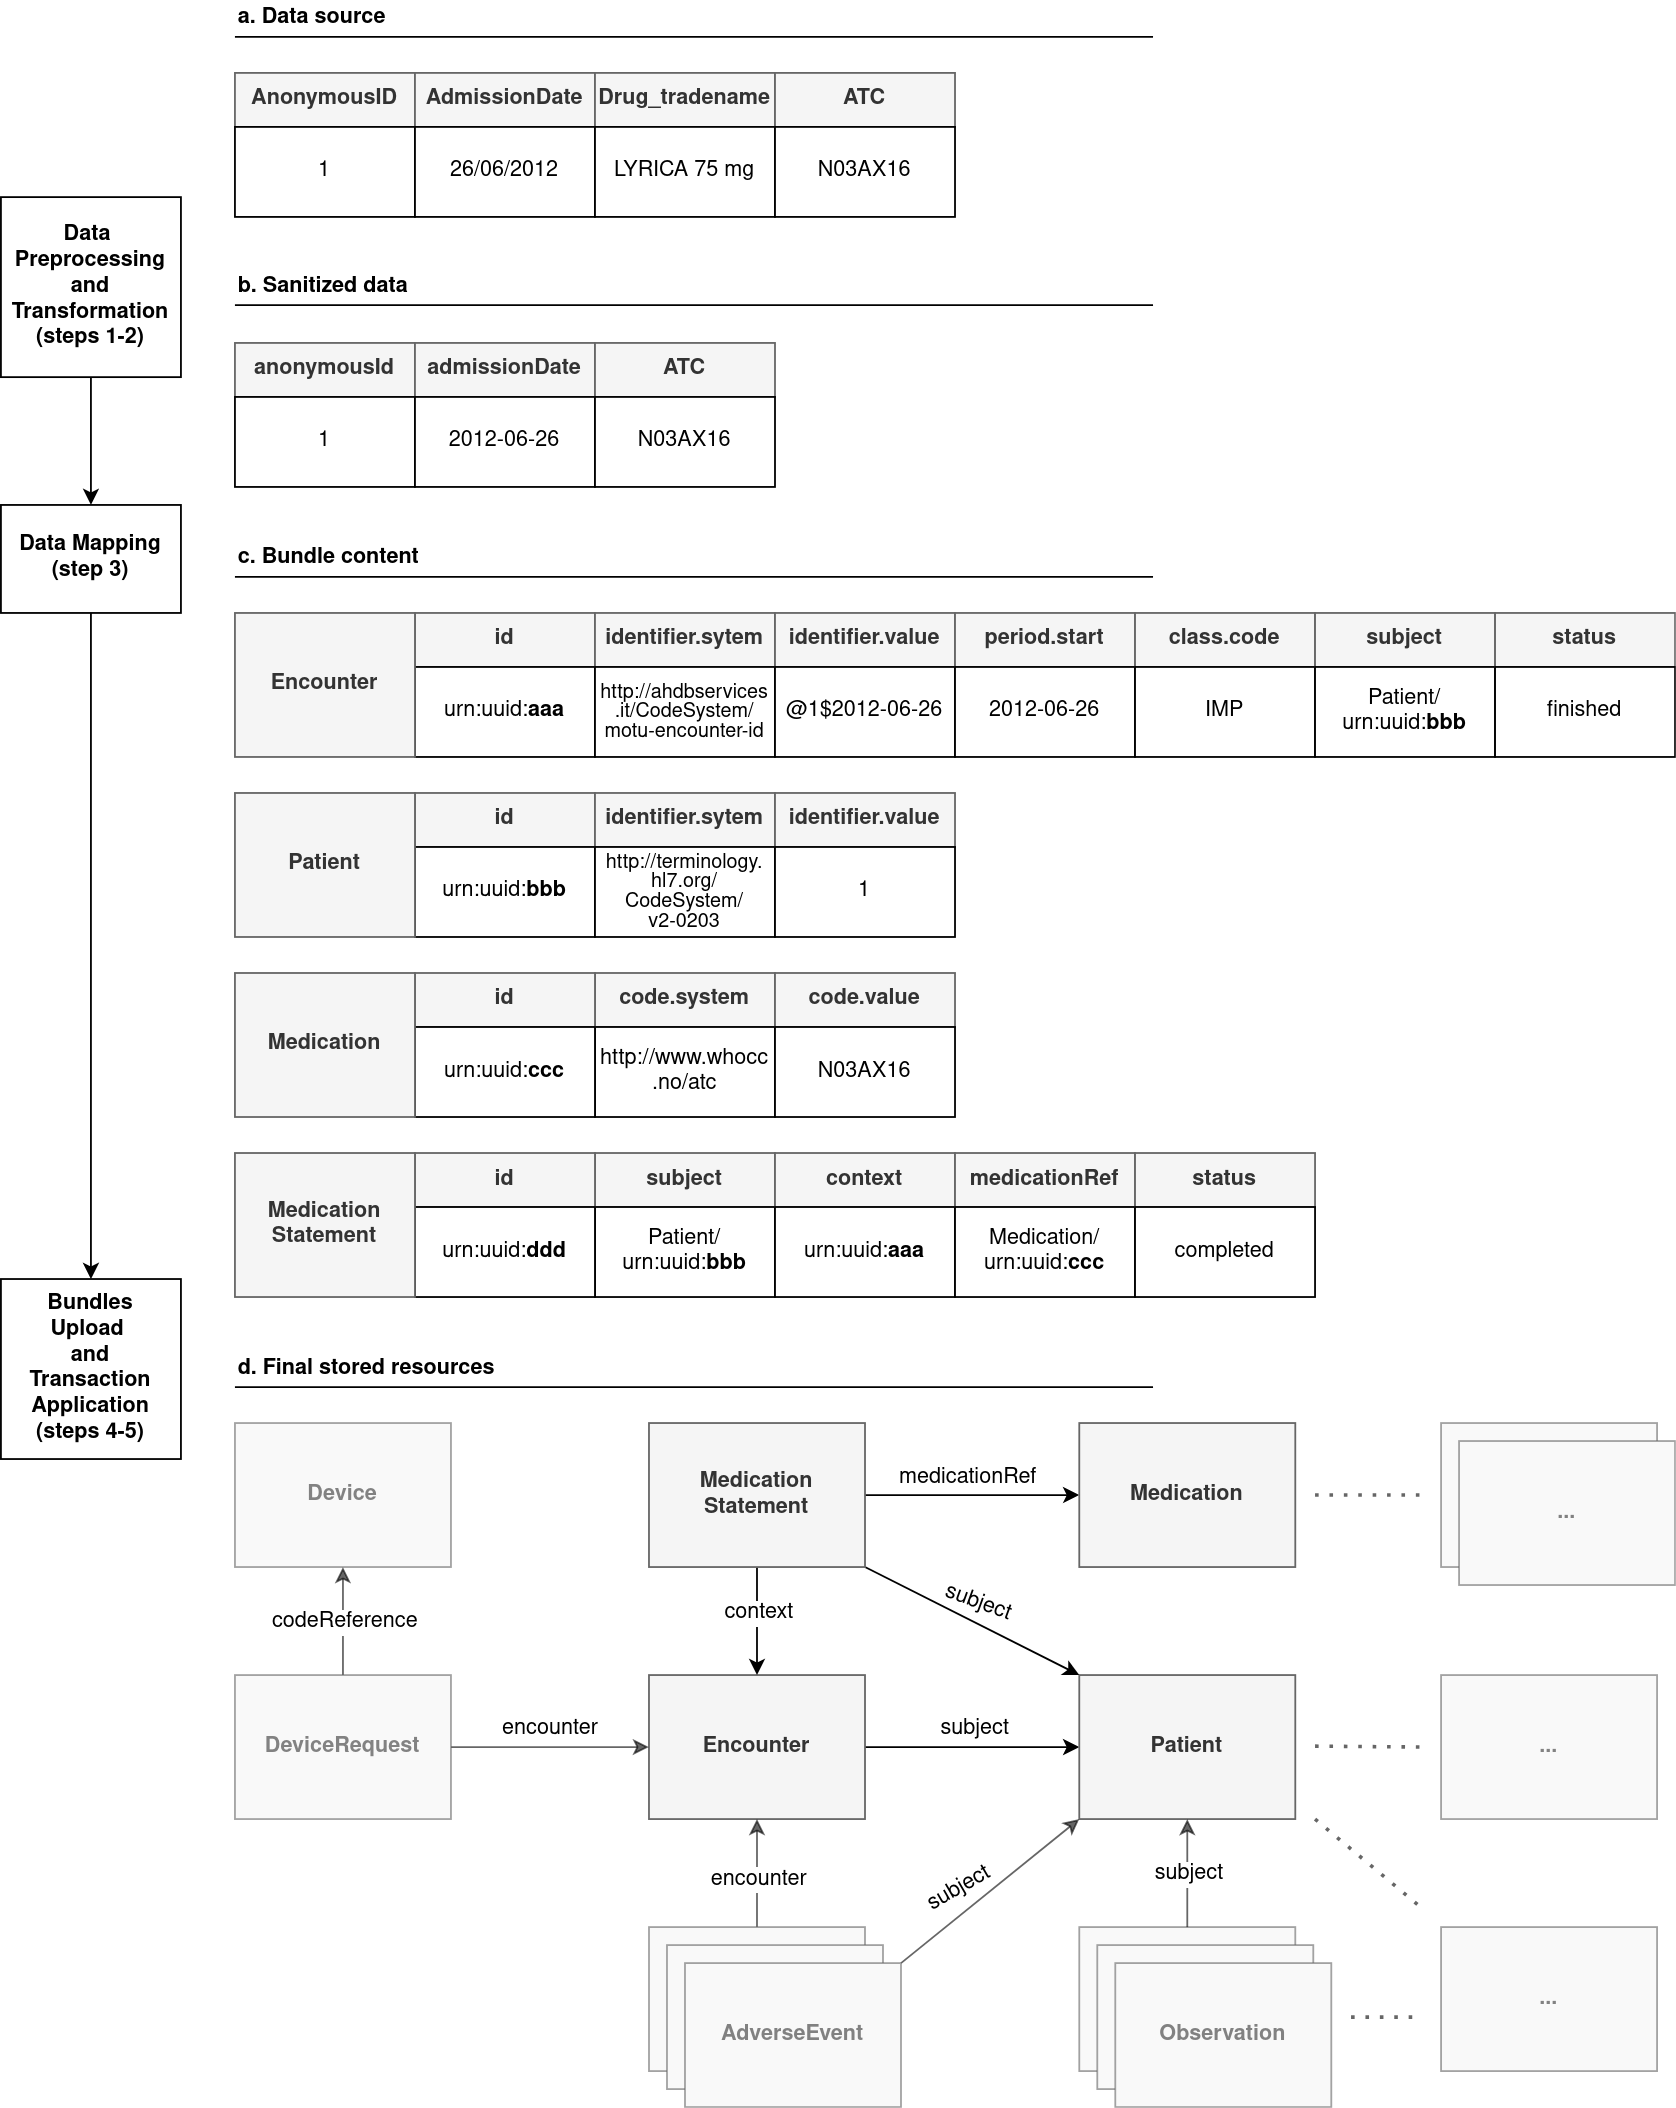
\includegraphics[width=\textwidth]{figures/paper2/4-data-conversion-workflow.png}}
%\caption{Simplified representation of a real-world example of data conversion workflow. It highlights all the crucial transformation steps from the source dataset (MOTU DrugHospitalStay table) to the FHIR domain. The resources produced in step 3 are implicitly organized inside a Bundle. Finally, in steps 4-5 the converted resources will be integrated with the prior knowledge.}
\caption{Diagram showing data conversion workflow from MOTU DrugHospitalStay table to FHIR domain, bundling resources in step 3, and integrating them with prior knowledge in steps 4-5."}
\label{paper2_5-data-conversion-workflow}
\end{figure}

\subsubsection{Implemented Mappings}

% \begin{table*}[t]
% \resizebox{\textwidth}{!}{%
% \begin{tabular}{|l|l|c|l|}
% \hline
% \textbf{MOTU} & \textbf{FHIR} & \textbf{Total resources} & \textbf{Usage} \\
% \hline
%  & Encounter & 1960 & Models the Information about the hospitalization of a patient \\
% \hline{1-3}
%  & QuestionnaireResponse & 23520 & Models the responses to standard questionnaires (Barthel, Morse, etc.) \\
%  & Account & 1960 &  \\
%  & Coverage & 1960 & \multirow{-2}{*}{Outline the entity in charge of payment} \\
%  & Observation & 11697 & Describes the measurements and the analysis results performed during the hospitalization \\
%  & Procedure & 1960 & Defines an intervention of amputation (body part, cause, date) \\
%  & Condition & 181 & Models any patient’s disorders, such as diabetes. \\
%  & DeviceRequest & 1835 & Model a request for knee prosthesis \\
%  & Careplan & 1960 &  \\
% \multirow{-10}{*}{HospitalStay} & Goal & 1960 & \multirow{-2}{*}{Describe the rehabilitation and the achieved goals} \\
% Knee & DeviceDefinition & 40 & Defines the properties of a certain model of knee prosthesis \\
%  & Medication & 370 &  \\
% \multirow{-2}{*}{Drug} & MedicationStatement & 3032 & \multirow{-2}{*}{Describe a drug and its prescriptions} \\
%  & AdverseEvent & 147 & Models a fall event associated with the hospitalization. \\
% \multirow{-2}{*}{Fall} & DocumentReference & 147 & Captures all the textual notes linked to the fall event \\
% Patient & Patient & 1005 & Models the patient's details \\\hline
% \end{tabular}%
% }
% \caption{Shows high-level mappings between MOTU tables and FHIR resources. These mappings establish a central reference point - Encounter, DeviceDefinition, Medication, AdverseEvent, and Patient - since it is referenced by all other resources derived from the same MOTU table's mapping process. }
% \label{tab:motu-references}
% \end{table*}

\begin{table*}[ht]
\resizebox{\textwidth}{!}{%
\begin{tabular}{|l|l|c|l|}
\hline
\textbf{MOTU} & \multicolumn{1}{c|}{\textbf{FHIR}} & \multicolumn{1}{c|}{\textbf{Total resources}} & \multicolumn{1}{c|}{\textbf{Usage}} \\ \hline
\multirow{10}{*}{HospitalStay} & Encounter & 1962 & Models the Information about the hospitalization of a patient \\ \cline{2-4} 
 & QuestionnaireResponse & 23544 & Models the responses to standard questionnaires (Barthel, Morse, etc.) \\ \cline{2-4} 
 & Account & 1962 & \multirow{2}{*}{Outline the entity in charge of payment} \\ \cline{2-3}
 & Coverage & 1962 &  \\ \cline{2-4} 
 & Observation & 11709 & Describes the measurements and the analysis results performed during the hospitalization \\ \cline{2-4} 
 & Procedure & 1962 & Defines an intervention of amputation (body part, cause, date) \\ \cline{2-4} 
 & Condition & 181 & Models any patient’s disorders, such as diabetes. \\ \cline{2-4} 
 & DeviceRequest & 1835 & Model a request for knee prosthesis \\ \cline{2-4} 
 & Careplan & 1962 & \multirow{2}{*}{Describe the rehabilitation and the achieved goals} \\ \cline{2-3}
 & Goal & 1962 &  \\ \hline
Knee & DeviceDefinition & 40 & Defines the properties of a certain model of knee prosthesis \\ \hline
\multirow{2}{*}{Drug} & Medication & 370 & \multirow{2}{*}{Describe a drug and its prescriptions} \\ \cline{2-3}
 & MedicationStatement & 3032 &  \\ \hline
Fall & AdverseEvent & 146 & Models a fall event associated with the hospitalization. \\ \hline
Patient & Patient & 1006 & Models the patient’s details \\ \hline
\end{tabular}%
}
\caption{Shows high-level mappings between MOTU tables and FHIR resources. These mappings establish a central reference point - Encounter, DeviceDefinition, Medication, AdverseEvent, and Patient - since it is referenced by all other resources derived from the same MOTU table’s mapping process.}
\label{tab:paper2_motu-references}
\end{table*}

% CHANGED: 
% The pipeline conversion process involves 157 fields of MOTU tables, covered by 15 distinct types of FHIR resources (Table \ref{tab:motu-references}).
% A correspondence with FHIR variables was found for 155 fields, representing 98.7\% of the dataset, of which 143 (91.1\%) were mapped to FHIR resources fields, and 12 identified as computable values through FHIRPath expressions.
% NEW:
The pipeline conversion process involves 157 fields from the MOTU tables, mapped to 15 distinct types of FHIR resources (Table \ref{tab:paper2_motu-references}). A correspondence to FHIR variables was established for 155 fields, covering 98.7\% of the dataset~\cite{arcobelli2024fhir}. Of these, 143 fields (91.1\%) were directly mapped to FHIR resource fields, while the remaining 12 (1.3\%) fields were recognized as computable values through FHIRPath expressions.
Several external ontologies, such as LOINC\footnote{https://loinc.org/}, SNOMED-CT\footnote{https://www.snomed.org/}, and Units of Measurement (UOM)\footnote{https://units-of-measurement.org/} ontology were adopted, to provide the results with a precise, consistent, and machine-readable representation of clinical concepts. As the information from the source dataset is specific, a corresponding concept from standard vocabularies was sometimes missing. Different Code Systems were created to overcome this lack of coverage. Moreover, before initiating the pipeline, shared concepts between all the records, such as Questionnaires, and Organizations were manually created and uploaded to the FHIR server. 

% CHANGED: 
% During our analysis of the dataset, we found redundant information in the source tables, such as the count of prescribed drugs during hospitalization. To avoid data duplication, inconsistencies, and potential errors, we decided not to include this information in the FHIR data model. We can still derive such pieces of information by using ad-hoc Search Parameters that incorporate FHIRPath expressions, which are accessible through the FHIR RESTful API.
% NEW:
% TODO: Controlla 157 variabili da dove vengono. Nel paragrafo sopra si parla di 75 fields.
% Of the initial 157 variables in the CSV dataset, we successfully established a correspondence with FHIR for 155 variables, representing 98.7\% of the dataset. We mapped 143 variables (91.1\%) to FHIR resources and identified 12 variables (1.3\%) that can be derived from FHIRPath expressions~\cite{moscato2024fhir}.

\subsubsection{Validation}
The validation process for resources derived from the MOTU dataset involved utilizing FHIRPath queries executed on the HAPI FHIR Server, and Python scripts for analyzing the original dataset. Initially, the validation encompassed counting the "root" resources, signifying overarching concepts uniquely identified by a primary key within the MOTU tables. This count was subsequently compared to the total number of rows within the tables, as outlined in Table \ref{tab:paper2_motu-convertion-results}. The consistent alignment of query counts across all assessments confirmed the accurate transformation of the core concepts of the MOTU domain. 
% CHANGED:
% In the validation test, utilizing queries provided by domain experts (Table \ref{tab:validation-queries}), we found consistent outcomes across both groups of queries (Table \ref{tab:motu-convertion-comparison}).
% NEW: attaccato paragrafo e cambiato "In the validation test" -> "Subsequently"
Subsequently, utilizing queries provided by domain experts (Table \ref{tab:paper2_validation-queries}), we found consistent outcomes across both groups of queries (Table \ref{tab:paper2_motu-convertion-comparison}).

% CHANGED:
% NEW:
% Identifying Relevant FHIR Elements for Data Quality Assessment in the German Core Data Set
% The OMOP common data model in Australian primary care data: Building a quality research ready harmonised dataset
% A Harmonized Data Quality Assessment Terminology and Framework for the Secondary Use of Electronic Health Record Data
% Development and initial validation of a data quality evaluation tool in obstetrics real-world data through HL7-FHIR interoperable Bayesian networks and expert rules
% Forse lo metterei in methodologies se diciamo che non sono verifiche, ma piu garanzie date dalla metodologia di lavoro


\begin{table}[ht]
\begin{tabular}{|l|l|c|c|}
\hline
\textbf{MOTU Table} & \textbf{FHIR Resource} & \textbf{No. MOTU} & \textbf{No. FHIR} \\ \hline
HospitalStay & Encounter & 1962 & 1962 \\ \hline
Knee & DeviceDefinition & 40 & 40 \\ \hline
Drug & MedicationStatement & 3035 & 3032* \\ \hline
Fall & AdverseEvent & 146 & 146 \\ \hline
Patient & Patient & 1006 & 1006 \\ \hline
\end{tabular}%
\caption{Comparison of distinct item counts in the original dataset and the corresponding FHIR “root” resources derived from mapping. Results are aligned, except for three MedicationStatement entries (*) excluded due to lacking ATC codes.}
\label{tab:paper2_motu-convertion-results}
\end{table}

% Please add the following required packages to your document preamble:
% \usepackage{graphicx}
% \usepackage[table,xcdraw]{xcolor}
% Beamer presentation requires \usepackage{colortbl} instead of \usepackage[table,xcdraw]{xcolor}
\begin{table}[ht]
\resizebox{\textwidth}{!}{%
\begin{tabular}{|l|c|c|}
\hline
\textbf{Query} & \textbf{Python count} & \textbf{SPARQL count} \\ \hline
Q1: How many patients who came for an initial supply return for a second hospitalization? & 85 & 85 \\ \hline
Q2: How many patients transition from the initial supply of a mechanical knee to a second supply of an electronic knee? & 34 & 34 \\ \hline
Q3: How many patients use anxiolytics/antidepressants (ATC Code: N06A and N05A) related to the risk of falls? & 67 & 67 \\ \hline
Q4:  Hospital stays from patients over 65 years old & 674 & 674 \\ \hline
Q5: How many falls per type of prosthesis (AMK, FK, etc.) & \begin{tabular}[c]{@{}l@{}}AMK - 11  \\ FK - 79  \\ LK - 26  \\ MPK - 28\end{tabular} & \begin{tabular}[c]{@{}l@{}}AMK - 11  \\ FK - 79  \\ LK - 26  \\ MPK - 28\end{tabular} \\ \hline
\end{tabular}%
}
\caption{Summary of results from demonstration queries. The total count for query Q5 is 144, reflecting the exclusion of two rows from the HospitalStay table due to the absence of any reference to the prosthesis model, leading to their omission in the inner join operation.}
\label{tab:paper2_motu-convertion-comparison}
\end{table}

% \begin{table}[]
% \resizebox{\textwidth}{!}{%
% \begin{tabular}{|l|l|l|}
% \hline
% \multicolumn{1}{|c|}{\textbf{DQA}} & \multicolumn{1}{c|}{\textbf{Description}}                           & \multicolumn{1}{c|}{\textbf{Implementation}}                                                                                                                                                                                                                                                  \\ \hline
% Value Conformance                  & Data values conform to allowed formats and values                   & \multirow{3}{*}{Adopting a FHIR Server with strict validation features ensures that data values conform to the correct formats, relational constraints are respected, and required values are always present, thus guaranteeing completeness and data integrity.}                             \\ \cline{1-2}
% Relational Conformance             & Data values conform to relational constraints and no duplicate keys &                                                                                                                                                                                                                                                                                               \\ \cline{1-2}
% Completeness                       & Absence of data under a predefined threshold                        &                                                                                                                                                                                                                                                                                               \\ \hline
% Computational Conformance          & Computed values conform to programming specification                & Computed values, like the number of medications, are not stored, as they can be derived dynamically using FHIRPath queries.                                                                                                                                                                   \\ \hline
% Uniqueness Plausibility            & There aren’t two or more resources that identify the same subject   & By adopting FHIR transactions for incremental updates, the risk of creating duplicate resources for the same patient is eliminated.                                                                                                                                                           \\ \hline
% Atemporal Plausibility             & Data measures are coherent to a local knowledge                     & \multirow{2}{*}{During the pre-processing phase, Python scripts with custom rules are used to validate input data, ensuring that temporal data adheres to expected time properties and that atemporal data is consistent with local knowledge and does not depend on time-sensitive factors.} \\ \cline{1-2}
% Temporal Plausibility              & Data measures are coherent with expected temporal properties        &                                                                                                                                                                                                                                                                                               \\ \hline
% \end{tabular}
% }%
% \caption{Implementation strategies for the Kahn framework data quality assessments (DQA).}
% \label{tab:kahn-indicators}
% \end{table}

\subsection{Discussion}\label{sec:paper2_discussion}
We successfully designed and implemented a modular FHIR-based conversion pipeline capable of extracting, preprocessing, and standardizing real-world health data.
Validation, performed on the MOTU dataset, ensures that the transformed data maintains accuracy and meaning. Consistent counts validated the preservation of core concepts, while clinician-driven queries affirmed the retention of semantic integrity and relational coherence. This comprehensive validation reinforces the trustworthiness of the transformed FHIR resources in capturing the essence of the MOTU domain. The resulting FHIR-conformant resources enhance interoperability, support high-throughput computation~\cite{hong_developing_2019}, and improve accessibility and readability for both humans and machines. This achievement is reinforced by the integration of standard ontologies, contributing to enriched semantic content and reduced ambiguities. Furthermore, the generated resources are efficiently findable through the RESTful Search API – a critical component for realizing a scalable platform capable of handling extensive volumes of information. Our harmonization process yields output with a greater volume than the input, attributable to the inclusion of metadata, mandatory fields, and references to external ontologies or concepts within FHIR resources. Managing this expanded knowledge corpus necessitates the deployment of automated software infrastructures, as emphasized in prior research~\cite{gehrmann_what_2023}. 

The implemented pipeline provides a versatile and scalable framework to support the FHIR modeling of custom data, including modules aimed at streamlining semi-automated data integration. The validation module removes the need for manual evaluation, cutting down time and reducing errors. This is pivotal for achieving semantic and structural interoperability in health information, identified as a significant research challenge in recent years~\cite{chatterjee_hl7_2022,kadakia_modernizing_2021}. As demonstrated with the MOTU dataset, this framework could play a crucial role in addressing a key aspect of digital health research — facilitating the comprehensive and meaningful reuse of real-world data. This capability is vital for supporting analyses in the field of Medical Data Science~\cite{gehrmann_what_2023}. 

In the realm of health informatics, the showcased pipeline exhibits several remarkable strengths that distinguish it from existing approaches. Primarily, its modular design ensures scalability and adaptability for a broad range of clinical studies and data sources, providing a versatile solution applicable across various scenarios. Notably, the adoption of Bundle transactions significantly enhances efficiency, enabling the processing of large datasets at speeds up to 50 times\footnote{https://smilecdr.com/docs/fhir\_standard/transactions.html} faster than individual operations. Furthermore, utilizing the RESTful interface provided by the FHIR server allows for parallel processing of bundles, further enhancing overall performance. 

An essential feature of the framework is its automated validation mechanism, systematically ensuring the adherence of each FHIR resource to the FHIR model. This procedure, supported by Structure Definitions and Structure Maps, distinguishes our study from others that rely on manual validation processes~\cite{montazeri2023developing}. Additionally, the adoption of a templating conversion strategy introduces a language-agnostic approach. This empowers users to concentrate exclusively on the mapping activity, irrespective of their technical proficiency. This eliminates the necessity for alterations to the framework code, allowing users to navigate the conversion process without requiring expertise in specific programming languages. 

Unlike similar solutions such as the .NET-based FHIR Converter\footnote{https://github.com/microsoft/FHIR-Converter}, limited to handling specific source data types (HL7 version 2 and CDA), our pipeline boasts versatility by accommodating any input format. In addition, adopting the FHIR Mapping Language not only formalizes the conversion process but also makes it externally accessible and publishable. This distinctive feature promotes transparency in our mappings, a quality often lacking in comparable studies~\cite{sinaci2023data,williams2023standardized}. 

The primary limitation of our research lies in its validation, which was exclusively conducted using the MOTU dataset. To enhance the robustness of our solution, our objective is to broaden the validation scope to encompass a wider range of datasets. This step is crucial for unveiling potential challenges and obstacles while assessing the practical adaptability of our pipeline architecture across diverse scenarios. For instance, it should be noted that, for the MOTU dataset, creating FHIR profiles was not necessary to handle explicit constraints given by domain-specific rules or requirements. On the contrary, other datasets may require the definition of FHIR profiles. As an example, the US Core FHIR profile\footnote{http://hl7.org/fhir/us/core/} provides its definitions for many FHIR resources, such as the Patient resource, which includes mandatory fields such as name and additional fields such as date of death, not natively mandatory in the basic Patient resource. The inclusion of FHIR profiles creation must be seamlessly integrated into our pipeline to map the structure and characteristics of the source information, avoiding any loss of context or meaning.

Other limitations arise from the current manual procedures for implementing ad-hoc input/refinement scripts and defining mappings. These tasks, inherently domain-specific, require substantial time and effort investment. A promising path for improvements involves exploring the implementation or integration of Natural Language Processing (NLP), as exemplified in Google's Healthcare Natural Language API\footnote{https://cloud.google.com/healthcare-api/docs/how-tos/nlp?hl=it }. NLP tools can be used to automatically extract structured data from unstructured clinical documents~\cite{hong_developing_2019} and to assist in creating mappings by suggesting the most suitable FHIR resources and external ontology codes to model specific concepts. In this regard, we are developing an automatic mapping tool that uses NLP to convert textual descriptions of variables into FHIR resources. By fine-tuning the model with FHIR documentation, the tool will act as a decision support system, suggesting outcomes that operators can review and approve. To enhance usability for non-technical users and streamline the process, these tools should feature a graphical user interface, ultimately saving time and simplifying the mapping workflow.

Finally, to enhance the efficiency of the overall post-hoc validation step, we are working on automation to streamline procedures. This involves integrating automated functionalities into a new pipeline module, aligned with DevOps principles. This module will orchestrate a series of tasks triggered by changes in mapping logic or source dataset. For instance, the generated FHIR resources will be converted directly into RDF format and integrated into a pre-deployed knowledge graph repository, like Apache Jena Fuseki. Afterward, predefined queries in configuration files will be analyzed against both input and output providing a comprehensive summary of results.
Automating these tasks facilitates seamless coverage and ensures consistent application of semantic integrity tests. Importantly, this approach decouples the technical implementation from the semantics of the queries outlined by non-technical users, significantly enhancing the acceptance process and pipeline usability.

\subsection{Conclusion}\label{sec:paper2_conclusion}
This paper presents an FHIR-based conversion pipeline designed to enhance the interoperability of real-world health data. The transition to a modern clinical standard, such as HL7 FHIR, represents a pivotal step towards unlocking latent value within heterogeneous data silos. Our solution, characterized by its modular architecture and templating mapping strategy based on the FHIR Mapping Language, offers a flexible and scalable approach to implementation, effectively addressing the complexities inherent in health data management. Furthermore, the employed templating approach ensures the formalization of mappings, providing an implementation-independent solution suitable for external publication. 
% CHANGED:
% NEW: attacca paragrafo
The effectiveness of our proposed solution underwent rigorous validation against the MOTU dataset. Through well-conceived queries on both the source dataset and the output generated by the pipeline, we demonstrated the pipeline's ability to seamlessly transform the MOTU dataset into FHIR without compromising accuracy or completeness.  

% CHANGED:
% Looking forward, future works involve the comprehensive validation of the pipeline across diverse datasets, considering variations in quality, format, and volume. As previously discussed, our emphasis lies in developing tools to streamline the mapping definition process, identified as a crucial bottleneck in the conversion workflow. By addressing these aspects, we aim to solidify the applicability and scalability of our FHIR-based conversion pipeline in real-world settings, effectively addressing prevailing challenges in health data interoperability. 
% NEW:
Building on these achievements, future efforts will prioritize expanding validation across diverse datasets, encompassing variations in structure, quality, and domain-specific requirements. Incorporating FHIR profile creation, where needed, will ensure that domain constraints are met without losing context or meaning. To address the manual bottlenecks in mapping and refinement, we plan to integrate advanced automation techniques, including natural language processing, to support variable extraction and mapping processes. Developing intuitive graphical interfaces for these tools will empower non-technical users, fostering broader adoption and usability.

Additionally, enhancing the automation of post-hoc validation through DevOps-aligned modules will streamline workflows, ensuring consistency and semantic coherence across all outputs. The incorporation of automated RDF conversion and semantic integrity tests within knowledge graphs will further reinforce the reliability of the pipeline while decoupling technical complexities from user interactions.

By addressing these aspects, we aim to solidify the applicability and scalability of our FHIR-based conversion pipeline in real-world settings, effectively addressing prevailing challenges in health data interoperability.

\subsection*{Acknowledgment}
This research was co-funded by the Complementary National Plan PNC-I.1 “Research initiatives for innovative technologies and pathways in the health and welfare sector” D.D. 931 of 06/06/2022, DARE - DigitAl lifelong pRevEntion initiative, code PNC0000002, CUP: 
(B53C22006450001) and by the Italian National Institute for Insurance against Accidents at Work (INAIL) within the MOTU++ project (PR19-PAI-P2). Authors express their gratitude to the AlmaHealthDB Team.

\subsection*{Code availability}
The MOTU-to-FHIR Mapping Pipeline code is available on GitLab at \url{https://gitlab.com/almahealthdb/ahdb-mapping-service/}. This repository includes all the necessary scripts, configuration files, and guidelines for converting the MOTU CSV dataset into a FHIRed dataset according to the HL7 FHIR standard (R4 version). It also offers a Docker Compose file configuring Matchbox and the HAPI FHIR Server, enabling automated pipeline deployment. For detailed instructions on running the pipeline, please refer to the README.md file in the repository.

% layout: keep this paper's floats within its section
\FloatBarrier



\chapter{Semantic Enrichment}
\label{chap:semantic_enrichment}

This chapter contains the two contributions associated with the \emph{Semantic Enrichment} stage described in Section~\ref{sec:semantic_enrichment}: Paper~3 (Section~\ref{sec:paper3}) and Paper~4 (Section~\ref{sec:paper4}). Together, they address RQ2, which is answered in Section~\ref{subsec:conclusions_rq2}.

% ============================================================================
% Paper 3 -- integrated from papers/meds_owl_JBI_2(1)/main.tex and supplementary.tex (front matter transcribed
% from the cas-dc \title/\author/\affiliation/\credit, abstract, graphical abstract and keywords; body converted
% mechanically, see the integration report). No bibliographic record for this paper was supplied, so it is not
% cited here.
% ============================================================================
\section{MEDS-OWL: An Ontology-Driven Framework for Clinical Outcome Prediction with Graph Learning}
\label{sec:paper3}

\paragraph{Authors.}
Alberto Marfoglia\textsuperscript{1,2,*}, Antonella Carbonaro\textsuperscript{1,*}, Adrien Coulet\textsuperscript{2,*}

{\raggedright % layout: ragged-right metadata block
\noindent\textsuperscript{1}Dept.\ of Computer Science and Engineering (DISI), University of Bologna, Bologna, Italy\\
\textsuperscript{2}Inria, Inserm, Universit\'e Paris Cit\'e, HeKA, UMR 1346, Paris, France\\
\textsuperscript{*}Corresponding author.\\
E-mail addresses: alberto.marfoglia2@unibo.it (A. Marfoglia), antonella.carbonaro@unibo.it (A. Carbonaro), adrien.coulet@inria.fr (A. Coulet).\\
URLs: \url{https://albertomarfoglia.github.io/} (A. Marfoglia), \url{https://www.unibo.it/sitoweb/antonella.carbonaro} (A. Carbonaro), \url{https://heka.gitlabpages.inria.fr/team/members/coulet.html} (A. Coulet).\\
ORCID: 0009-0000-5857-2376 (A. Marfoglia), 0000-0002-3890-4852 (A. Carbonaro), 0000-0002-1466-062X (A. Coulet).
\par}

{\raggedright
\noindent\textsuperscript{a}Dept. of Computer Science and Engineering (DISI), University of Bologna, Bologna, Italy\\
\textsuperscript{b}Inria, Inserm, Universit\'e Paris Cit\'e, HeKA, UMR 1346, Paris, France\\
\textsuperscript{*}Corresponding authors.\\
Preprint submitted for publication in the Journal of Biomedical Informatics. Available at SSRN: \url{https://papers.ssrn.com/sol3/papers.cfm?abstract_id=7545256}.\\
\par}

\subsection*{Abstract}

Objective: To develop a formal semantic representation of the Medical Event Data Standard (MEDS), an event-centric standard for structured clinical data, using Semantic Web technologies and supporting reproducible graph-based machine learning. We further investigate how the semantic granularity of the resulting graph representation affects clinical outcome prediction.\\
Methods: We present MEDS-OWL, a lightweight ontology that extends MEDS with a formal semantic representation, together with \texttt{meds2rdf}, a scalable Python library for transforming MEDS-compliant datasets into FAIR-aligned MEDS-RDF graphs. Round-trip fidelity and scalability were evaluated on four heterogeneous clinical datasets (NEUROVASC, MIMIC-IV, eICU, and NWICU), comprising more than 309,000 hospital stays. For downstream evaluation, 11 prediction tasks derived from MIMIC-IV were formulated as patient-level binary classification problems. A two-layer Relational Graph Convolutional Network with literal-aware encoding was evaluated across three MEDS-RDF schema variants differing in subject–event predicate granularity, enabling systematic assessment of the influence of representation granularity on graph-based learning.\\
Results: The framework preserved structural completeness and the core MEDS fields with high fidelity across the four datasets. Its streaming conversion architecture enabled processing RDF graphs of up to 937 GB, achieving a 2.7$\times$ speedup over its predecessor. Across the 11 prediction tasks, increasing semantic granularity from MEDS-RDF-Base to Partial to Full consistently improved Macro-F1, narrowing the performance gap with tabular baselines.\\
Conclusions: MEDS-OWL provides a scalable, interoperable, and FAIR-aligned framework for representing MEDS data as semantic clinical graphs. The results demonstrate that semantic representation extends beyond interoperability and therefore should be treated as an important determinant of graph-based clinical machine learning performance in predictive analytics for clinical outcomes.

\subsection*{Graphical abstract}

\begin{center}
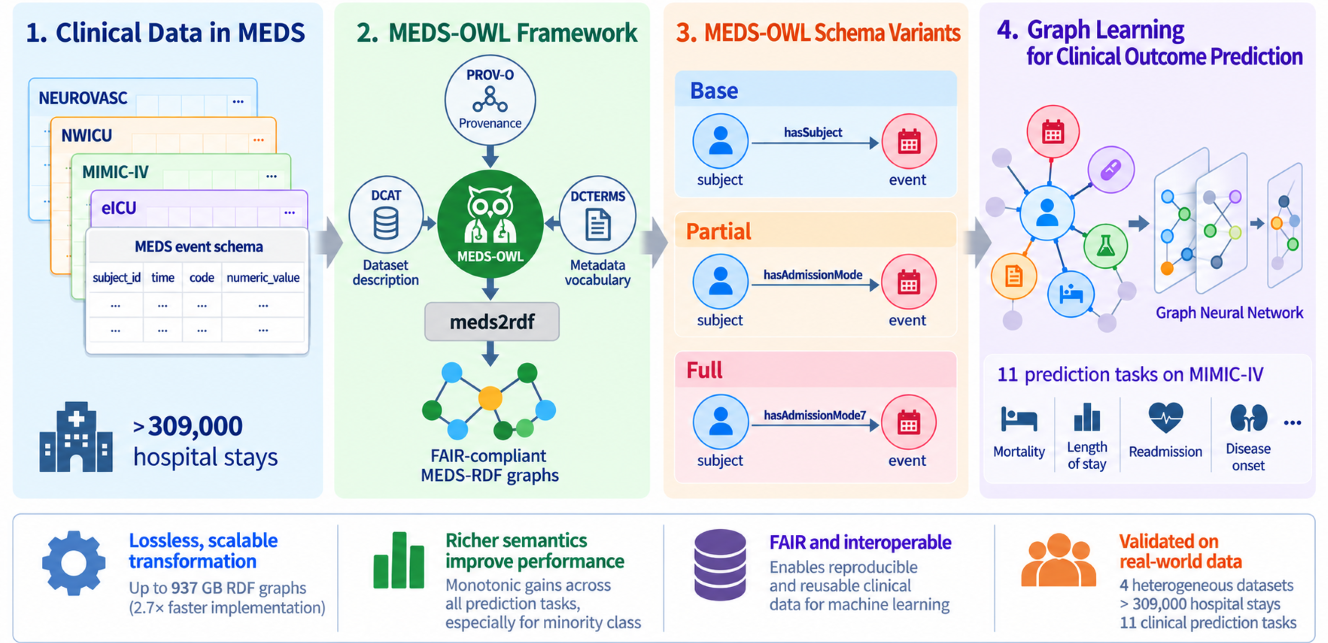
\includegraphics[width=\textwidth]{figures/paper3/graphical_abstract.png}
\end{center}

\paragraph{Keywords:} Medical Event Data Standard (MEDS); Knowledge graph; OWL ontology; Graph Convolutional Network; Healthcare; Predictive machine learning; FAIR principles

\subsection{Introduction}
Machine learning (ML) in healthcare is hindered by the lack of standardized representations for structured Electronic Health Record (EHR) data, resulting in dataset-specific preprocessing practices, limited reproducibility, and poor model portability across datasets. The Medical Event Data Standard (MEDS)~\cite{bert_arnrich_medical_2024,mcdermott_meds_2024} addresses this gap by introducing a unified, event-centric schema for longitudinal health data that is explicitly designed to support reproducible and efficient ML workflows. MEDS represents each clinical event using a minimal tuple consisting of a subject identifier, a code, and optional temporal and value attributes. This lightweight and pragmatically oriented design makes MEDS suitable for benchmarking, multi-center studies, and the development of foundation models. Accordingly, MEDS has been adopted in several ML projects; for example, it has been used to train transformer-based models for predicting future events in patient healthcare trajectories~\cite{renc_foundation_2025,oufattole_meds-tab_2024}.

In its native form, MEDS is a data-format specification and does not provide ontology-level semantics. The Semantic Web paradigm offers a complementary approach to address this limitation~\cite{hitzler_foundations_2009,MARFOGLIA2026108380}. Ontologies expressed using Resource Description Framework (RDF) and Web Ontology Language (OWL) provide machine-interpretable and interoperable representations of entities and their relationships, while supporting semantic querying and formal reasoning. They also enable the construction of knowledge graphs (KGs), facilitating the explicit linkage of dataset elements to external terminologies such as LOINC, SNOMED CT, or ATC~\cite{hogan_knowledge_2021}. 

Projecting MEDS datasets into RDF would thus facilitate their semantic integration and validation while creating opportunities for graph-based ML on longitudinal clinical data. By explicitly representing subjects, events, and their relationships as a graph, such representations can be processed using ML methods that exploit relational structure\cite{schlichtkrull_2018}. Despite the growing use of clinical KGs and graph neural networks, the effect of semantic representation granularity on graph-based clinical prediction has received limited systematic investigation.

In this study, we propose a semantic framework for representing MEDS-based clinical data as interoperable and FAIR-aligned graphs. This work is the first to (i) formalize a general-purpose OWL ontology named MEDS-OWL for the MEDS standard, (ii) develop a scalable, streaming MEDS-RDF conversion library validated at production scale, named \texttt{meds2rdf}, and (iii) demonstrate the utility of the MEDS-OWL representation for clinical outcome prediction on real-world data by systematically varying predicate granularity as an independent variable in graph-based predictive modeling.

\begin{table}[htbp]
\centering
\begin{tabular}{p{0.2\textwidth} p{0.8\textwidth}}
\hline
\textbf{Problem or Issue} &
MEDS provides a standardized event-centric format for clinical data, but lacks ontology-level semantics, limiting semantic interoperability and leaving the effect of representation granularity on graph-based prediction unclear.
\\[0.5em]

\textbf{What is Already Known} &
RDF and clinical knowledge graphs support interoperability, provenance, semantic querying, and graph-based learning, but existing representations are often tailored to specific data models, infrastructures, or use cases.
\\[0.5em]

\textbf{What this Paper Adds} &
We introduce MEDS-OWL, a general-purpose OWL ontology for MEDS, and meds2rdf, a scalable streaming framework for generating FAIR MEDS-RDF graphs. We further systematically evaluate how subject-event predicate granularity affects graph-based clinical outcome prediction across 11 MIMIC-IV tasks.
\\[0.5em]

\textbf{Who would benefit from the new knowledge in this paper} &
Clinical informatics researchers, biomedical data scientists, and machine-learning researchers working with interoperable, reproducible graph representations of longitudinal clinical data.
\\
\hline
\end{tabular}
\end{table}
%
%
%
%
%

\subsection{Related Work}
\label{sec:paper3_related_work}
%
While several data models and ontologies, such as FHIR~\cite{lehne_use_2019}, OMOP CDM~\cite{xiao_fhir-ontop-omop_2022}, and Phenopackets~\cite{kaliyaperumal_phenopackets_2022}, have been proposed to harmonize clinical data, RDF transformations of these models have seen limited adoption~\cite{xiao_fhir-ontop-omop_2022,marfoglia_towards_2025}, in part due to loosely specified semantics or incomplete coverage of the clinical domain.
Patient-centric RDF-based representations such as SPHN~\cite{toure2023} and CARE-SM~\cite{kaliyaperumal_semantic_2022} illustrate how KGs can facilitate interoperability, provenance modeling, and temporal reasoning.
However, these models are often tightly coupled to specific use cases or semantic frameworks.

KGs provide a natural representation for clinical data in which patients, events, concepts, and their relationships can be represented explicitly. KG embeddings map graph nodes and edges into continuous vector spaces, enabling relational structures to be incorporated into computational models~\cite{hamilton_representation_2018}. Such representations have been applied to tasks including link prediction, node classification, and clustering~\cite{wang_knowledge_2017}. Graph neural networks extend these ideas by learning representations directly from graph structure. In particular, Relational Graph Convolutional Networks (RGCNs) have been shown good performances when the underlying schema aligns with task-specific requirements~\cite{schlichtkrull_2018}; for instance, compact and patient-centered representations for outcome prediction \cite{MARFOGLIA2026108380}. 

MEDS-OWL addresses these gaps by providing a semantic representation of a data model specifically designed for ML research in healthcare. It preserves the compact, event-centric design of MEDS while adding ontology-level semantics, combining representation compactness with semantic expressiveness. This positions MEDS-OWL as a semantic foundation for FAIR clinical graphs while retaining the practical properties required for scalable ML workflows.

\subsection{Methods}\label{sec:paper3_methods}
In this section, we first describe the development of the MEDS-OWL ontology and of the \texttt{meds2rdf} library (Section~\ref{sec:paper3_meds-owl-design}). Second, we introduce the datasets and the semantic enrichment mechanism used to generate three MEDS-RDF schema variants of increasing semantic granularity (Section~\ref{sec:paper3_enrichment}). Finally, we present the clinical prediction tasks and the GNN-based predictive strategy used to evaluate the impact of these schema variants, including a tabular baseline and SHAP-guided pruning procedure that support their evaluation (Section~\ref{sec:paper3_prediction-task}), followed by the end-to-end experimental pipeline (Section~\ref{sec:paper3_exp-pipeline}).


\subsubsection{MEDS-OWL ontology, \texttt{meds2rdf} library and  MEDS-RDF datasets}
\label{sec:paper3_meds-owl-design}

\paragraph{Ontology Development Process.}\label{sec:paper3_ontology_development}
MEDS-OWL~\cite{marfoglia_teamhekameds-ontology_2025} was developed following the ontology-engineering methodology of Noy and McGuinness~\cite{mcguninnes}, using Protégé~\cite{musen_protege_2015}. It represents EHR- and claims-style medical events defined by MEDS together with dataset- and experiment-level metadata for reproducible ML workflows. The ontology defines seven core classes: \texttt{Subject}, \texttt{Event}, \texttt{Code}, \texttt{DatasetMetadata}, \texttt{SubjectSplit}, \texttt{SubjectLabel},
and \texttt{ValueModality}. A detailed description of the ontology design nd development process is provided in \cite{marfoglia_clinical_2026}; the correspondence with MEDS schema components and complete class descriptions are reported in Suppl. Tables~\ref{tab:paper3_schema-to-ontology} and \ref{tab:paper3_meds-owl-concepts}, respectively.

\paragraph{MEDS-RDF Generation Library: \texttt{meds2rdf}.}\label{sec:paper3_meds2rdf}
We developed \texttt{meds2rdf}~\cite{marfoglia_teamhekameds2rdf_2025}, a Python library implementing the mapping from MEDS datasets to
MEDS-OWL-compliant RDF graphs. The first release constructed the complete graph in an in-memory \texttt{rdflib.Graph}, which limited scalability for large EHR datasets. The second release introduces a \emph{sink-based} architecture that decouples triple generation from storage. Triples are generated incrementally as MEDS partitions are processed and passed to a \texttt{TripleSink} implementation. Two sinks are provided: \texttt{GraphSink}, which preserves the in-memory \texttt{rdflib.Graph} workflow for small datasets and testing, and \texttt{NTriplesSink}, which streams triples directly to disk in N-Triples format, with optional gzip compression and configurable batching. The latter avoids retaining the complete graph in memory and is intended for large-scale datasets.
Additional storage backends can be implemented by extending the \texttt{TripleSink} interface.

\paragraph{Conversion Workflow.}\label{sec:paper3_end-to-end-worflow}
Figure~\ref{fig:paper3_meds-to-rdf-etl} summarizes the end-to-end MEDS-RDF conversion workflow. (a) When source data are not already in MEDS format, \texttt{MEDS-extract}~\cite{mcdermott_meds_2024} first applies a declarative conversion template to generate MEDS event tuples. This step is optional for datasets already conforming to MEDS. (b) The resulting MEDS data are then transformed into MEDS-RDF using \texttt{meds2rdf}, whose deterministic, table-driven mappings associate MEDS schema elements with the corresponding MEDS-OWL classes and properties. (c) Generated triples are incrementally passed to the selected \texttt{TripleSink}. For \texttt{GraphSink} outputs, optional SHACL validation using \texttt{pySHACL} checks the semantic constraints encoded by MEDS-OWL
before serialization to standard RDF formats. This separation of mapping and validation allows ontology constraints to evolve independently from the conversion implementation; further details are provided in the Supplementary Methods.

\begin{figure*}[h]
  \centering
  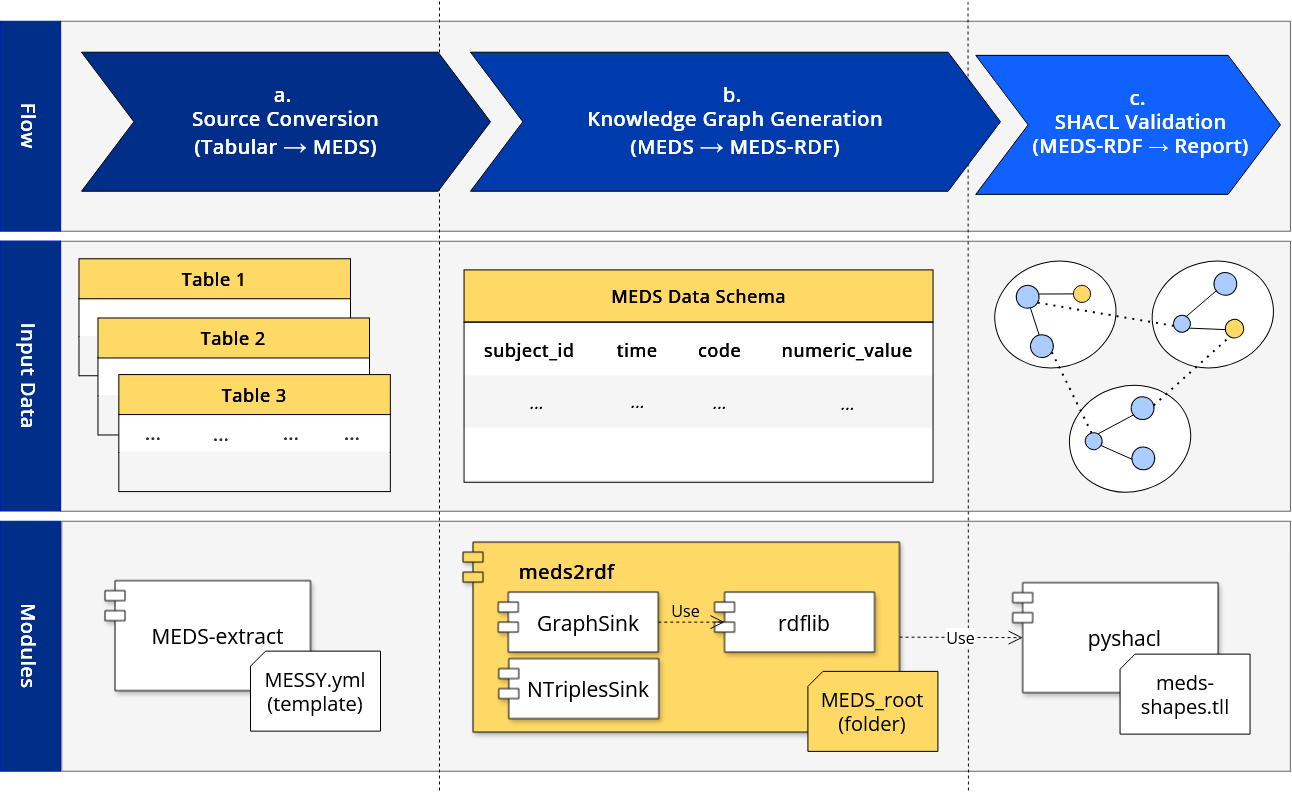
\includegraphics[width=\textwidth]{figures/paper3/fig0.png}
  \caption{Overview of the end-to-end MEDS-RDF transformation pipeline, illustrating (a) normalization and extraction of tabular data into MEDS event tuples, optional if data are already in MEDS, (b) transformation into MEDS-RDF KGs compliant with the MEDS-OWL ontology, and (c) optional SHACL-based validation and serialization into standard RDF formats.}
  \label{fig:paper3_meds-to-rdf-etl}
\end{figure*}
%
%
\paragraph{Evaluation Datasets.}\label{sec:paper3_datasets}
% \begin{table}[h]
% \caption{Datasets, with MEDS ETL support, used for evaluation. %All real-world datasets require credentialed access via PhysioNet. MEDS ETL links point to publicly available conversion pipelines
% }\label{tab:datasets}
% \begin{tabular*}{\tblwidth}{@{}L@{}R@{}C@{}C@{}C@{}}
% \toprule
% \textbf{Dataset} & \textbf{$\sim$ Stays} & \textbf{Version} &
% \textbf{Origin} & \textbf{Published}
% \\ % Table header row
% \midrule
% NEUROVASC & 10,000  & v1.0  & France & 2025  %& Synthetic care-pathway cohort for ruptured intracranial aneurysm patients
% \\
% NWICU     & 25,000  & v0.1.0 
% & USA    & 2023  %& Single-centre ICU database from Northwestern Memorial Hospital 
% \\
% MIMIC-IV  & 73,000  & v3.1   
% & USA    & 2020  %& Single-centre ICU database from Beth Israel Deaconess Medical Center 
% \\
% eICU      & 201,000 & v2.0  & USA    & 2017  %& Multi-centre ICU database spanning 208 US hospitals 
% \\

% \bottomrule
% \end{tabular*}
% \end{table}
We evaluated the MEDS-OWL framework on four datasets. NEUROVASC \cite{jhee_predicting_2025} is a synthetic open cohort describing care pathways of 10,000 patients hospitalised for ruptured intracranial aneurysms, generated from real-world EHR data at Nantes University Hospital, France. eICU \cite{pollard_eicu_2018} is a large multi-centre ICU database comprising approximately 201,000 admissions. MIMIC-IV \cite{johnson_mimic-iv_2023} contains de-identified EHR data for about 73,000 ICU stays and is one of the most widely used benchmarks in clinical informatics. NWICU \cite{moukheiber_northwestern_2024} is a single-centre ICU database covering approximately 25,000 stays. Access to eICU, MIMIC-IV, and NWICU requires credentialed PhysioNet registration and completion of a data-use agreement.

\paragraph{Round-Trip Fidelity Evaluation.}\label{sec:paper3_fidelity}
To assess whether the MEDS-RDF transformation preserves information faithfully, beyond the structural statistics reported in Section~\ref{sec:paper3_usage-examples}, we conducted a \emph{round-trip fidelity} evaluation across all four datasets. For each dataset, we (\textit{i}) converted five independent subsamples, each comprising MEDS events from 100 randomly selected patients, to RDF using \texttt{meds2rdf}, (\textit{ii}) reconstructed a tabular representation from the resulting RDF graph, and (\textit{iii}) compared the reconstructed data with the original MEDS source in terms of structural completeness and field-level fidelity. Detailed sampling procedures, metric definitions, and matching criteria are provided in the Suppl. Section \ref{sec:paper3_supp-fidelity}. The resulting fidelity measures are reported in Section~\ref{sec:paper3_evaluate-meds-rdf-conversion}.

\subsubsection{Graph Representation of Clinical Events}\label{sec:paper3_enrichment}
MEDS-RDF represents clinical events using \texttt{meds:hasSubject}, \texttt{meds:hasCode}, \texttt{meds:codeString}, and \texttt{meds:*Value} (Suppl. Table~\ref{tab:paper3_events}). In the base representation, all subject--event links use the generic \texttt{meds:hasSubject} predicate. To investigate how semantic granularity affects graph representation, \texttt{meds2rdf} provides a lightweight enrichment mechanism that specializes only the generated RDF instances, leaving the MEDS-OWL ontology unchanged. It derives more specific subject--event predicates from the event code string, which uses the \texttt{//} separator to encode progressively finer event information, as in \texttt{ATC//C08CA06} or \texttt{ICD//10//OBH17EZ}. This yields three representation variants (Figure~\ref{fig:paper3_meds-rdf-variants}): \emph{MEDS-RDF-Base}, which retains the generic \texttt{meds:hasSubject} relation; \emph{MEDS-RDF-Partial}, which specializes the relation using the event type before the first \texttt{//}; and \emph{MEDS-RDF-Full}, which further incorporates the complete code string, including the value-bearing segment.

For the enriched variants, predicates are generated deterministically by splitting the code string on non-alphanumeric delimiters, converting the resulting tokens to camelCase, and prefixing them with \texttt{has}. Codes without \texttt{//} produce identical Partial and Full predicates, while for codes containing multiple \texttt{//} separators, only the first separates the event type from the remaining code; subsequent separators are replaced with underscores to form valid normalized URIs.

% \subsection{Graph Representation of Clinical Events}\label{sec:enrichment}
% In MEDS-RDF, clinical events are represented using the predicates \texttt{meds:hasSubject}, \texttt{meds:hasCode}, \texttt{meds:codeString}, and \texttt{meds:*Value} (see Suppl. Table~\ref{tab:events}). While event attributes are explicitly modeled, the relation connecting a subject to an event is, in the base formulation, a single undifferentiated predicate (\texttt{meds:hasSubject}) that is shared across all event types.
% To investigate the effect of semantic granularity in graph construction, we introduce a lightweight semantic enrichment mechanism in \texttt{meds2rdf}. This mechanism refactors only the generated RDF instances, leaving the MEDS-OWL ontology unchanged, and replaces the generic subject--event relation with more specific predicates derived from the string associated with event codes. Such codes are of the form "event\_type//event\_subtype" where the separator // separates various levels of details of the event such as in "ATC//C08CA06" or "ICD//10//OBH17EZ". Our use of this specialisation of predicates yields three graph representation variants with increasing levels of semantic specificity, as illustrated in Figure~\ref{fig:meds-rdf-variants}:
% \begin{itemize}
%   \item \textbf{MEDS-RDF-Base}: the standard representation aligned with MEDS-OWL, where all subject--event links are expressed via \texttt{meds:hasSubject}.
%   \item \textbf{MEDS-RDF-Partial}: the subject--event relation is specialized using the event type, obtained from the code string segment preceding the first occurrence of the \texttt{//} separator.
%   \item \textbf{MEDS-RDF-Full}: the relation is further specialized using the complete code string, including the value-bearing segment following the last \texttt{//}, producing predicates that encode both event type and value.
% \end{itemize}

% For both enriched variants, predicates are automatically generated by \texttt{meds2rdf} through a deterministic transformation that splits code strings on non-alphanumeric delimiters, converts the resulting tokens to camelCase, and prefixes them with \texttt{has}. In the absence of a value segment (i.e., codes without the \texttt{//} delimiter), the partial and full variants coincide. In the case of more than one \texttt{//} delimiter, only the first is treated as the separator between the code and value segments; all subsequent occurrences are replaced with underscores (\texttt{\_}) to produce a valid, normalized URI.
% %Figure~\ref{fig:meds-rdf-variants} illustrates the three representations for the same example event, highlighting how progressively richer predicate semantics modify the structure of the resulting graph.
 
\begin{figure*}[h]
  \centering
  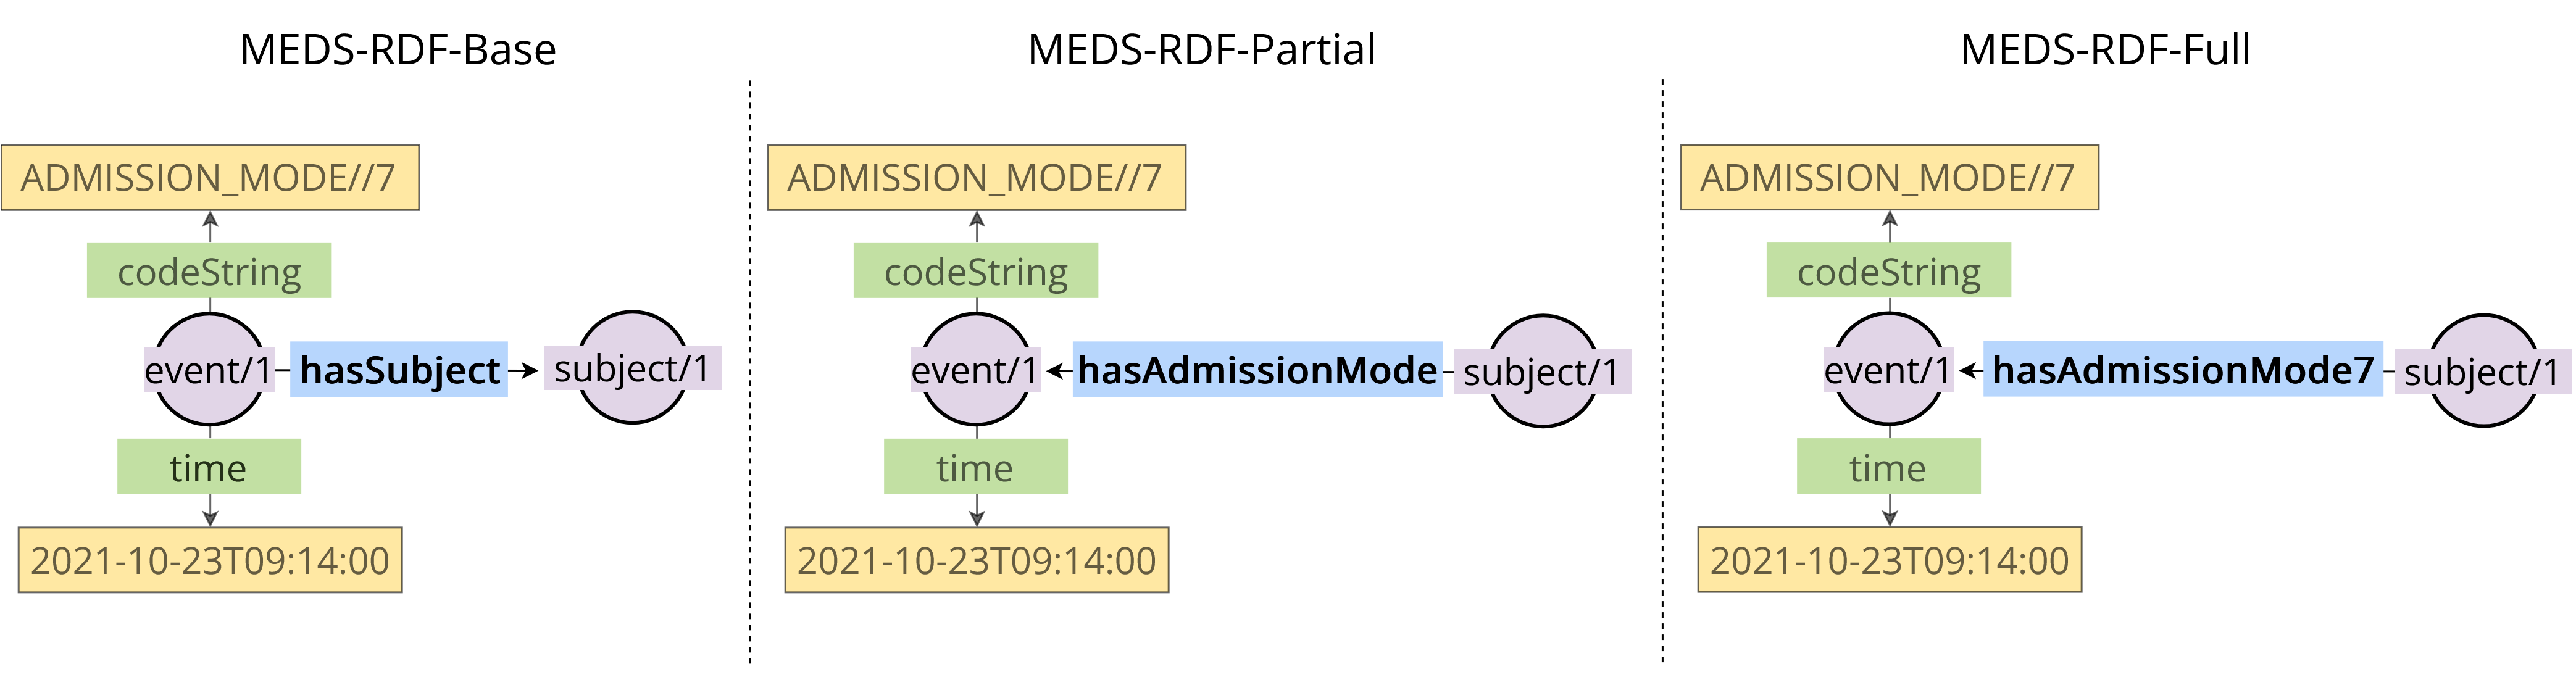
\includegraphics[width=\textwidth]{figures/paper3/fig5.png}
  \caption{MEDS-RDF representation variants of the same event (\texttt{Admission\_Mode//7}) under the three subject--event linking strategies.}
  \label{fig:paper3_meds-rdf-variants}
\end{figure*}
 
\subsubsection{Patient Outcome Prediction}\label{sec:paper3_prediction-task}
\paragraph{Prediction Tasks.}
To evaluate whether MEDS-RDF schema granularity affects downstream clinical prediction, and whether such effects generalize, we construct a multi-task predictive benchmark over MIMIC-IV using the 11 prediction tasks in Table~\ref{tab:paper3_mimic-tasks}. These latter are common prediction tasks, and we reproduce them by leveraging the ACES (Automatic Cohort Extraction System) definitions published by \cite{mcdermott_mimic-iv_2025} (see Section~\ref{sec:paper3_exp-pipeline}, Stage 2, for details). Each task is cast as a node classification problem over the corresponding MEDS-RDF graph, with patient nodes labelled according to the task-specific binary outcome. 
%
\begin{table*}[h]
\centering
\caption{A collection of various common predictive tasks on MIMIC-IV~\cite{mcdermott_mimic-iv_2025}}
\label{tab:paper3_mimic-tasks}
\begin{tabular}{p{4.8cm} p{8.4cm}}
\hline
\textbf{Task Name} & \textbf{Description} \\
\hline
First 24h in-hospital mortality & Predict mortality within a hospital admission using the first 24 hours of data from that admission. \\
First 48h in-hospital mortality & Predict mortality within a hospital admission using the first 48 hours of data from that admission. \\
First 24h in-ICU mortality & Predict mortality within an ICU admission using the first 24 hours of data from that admission. \\
First 48h in-ICU mortality & Predict mortality within an ICU admission using the first 48 hours of data from that admission. \\
Hospital LOS $>$3 days & Predict a hospital length of stay greater than 3 days, using the first 48 hours of data after admission.%, with a 24-hour gap between the input and target windows; patients who die or are discharged during the gap window are excluded. \\
\\
ICU LOS $>$3 days & Predict an ICU length of stay greater than 3 days, using the first 48 hours of data after ICU admission.%, with a 24-hour gap between the input and target windows; patients who die or are discharged during the gap window are excluded. \\
\\
30d post-hospital-discharge mortality & Predict mortality within 30 days after discharge. \\
1y post-hospital-discharge mortality & Predict mortality within 1 year after discharge. \\
30d re-admission & Predict hospital readmission within 30 days of discharge. \\
Myocardial infarction 1--5Y phenotyping & Predict myocardial infarction (MI) incidence 1--5 years after an hospital admission. \\
CKD onset in diabetics 5Y from kidney panel & Predict chronic kidney disease (CKD) onset in diabetic patients within 5 years of any kidney panel laboratory test. \\
\hline
\end{tabular}
\end{table*}
 %
 %
 
\paragraph{Architecture.}

We use a Relational Graph Convolutional Network (RGCN)~\cite{schlichtkrull_2018} as a common downstream model for all experiments, because it has been shown to provide competitive performance for entity classification against alternative graph-based approaches~\cite{schlichtkrull_2018}. We keep the architecture, hyperparameters, and training protocol fixed across graph variants, so that schema granularity (MEDS-RDF-Base, -Partial, and -Full) is the only experimental variable. RGCN is well suited to this comparison because it uses relation-specific transformations for different relation types and directions~\cite{schlichtkrull_2018}, making the learned representations sensitive to differences in predicate specialization.

For a graph $G = (\mathcal{V}, \mathcal{E}, \mathcal{R}, \mathcal{X})$ with node set $\mathcal{V}$, edge set $\mathcal{E}$, relation set $\mathcal{R}$, and initial embeddings $\mathcal{X} \in \mathbb{R}^{n \times d_0}$, the first-layer representation of target (patient) node $i$ is
\[
h_i^{(1)} =
\sigma
\left(
\sum_{r \in \mathcal{R}}
\sum_{j \in \mathcal{N}_i^r}
\frac{1}{c_{i,r}}
W_r^{(0)} x_j
+
W_0^{(0)} x_i
\right),
\]
where $\mathcal{N}_i^r$ is the neighborhood of $i$ under relation $r$, $c_{i,r}$ a normalization constant, $W_r^{(0)}$ the relation-specific weights, $W_0^{(0)}$ the self-connection weight, and $\sigma$ a nonlinear activation. We apply basis-decomposition regularization~\cite{schlichtkrull_2018} ($B=8$) to control parameter growth, which is especially important for MEDS-RDF-Full given its larger relation set. 

Since MEDS-RDF encodes attributes such as age and lab values as RDF literals, we adopt the RGCN+Literals extension~\cite{kristiadi_incorporating_2019}: literals are mapped to dense vectors via an MLP, $x_{\mathrm{literal}} = \sigma(Wv+b)$, and inserted into $\mathcal{X}$ before message passing.

After $L$ RGCN layers, each patient node $p \in \mathcal{P}$ is projected to a scalar logit $h_p$, trained with binary cross-entropy against the clinical outcome. Suppl. Figure~\ref{fig:paper3_rcgn+lit} shows the overall architecture.

\paragraph{Implementation.} We implement a two-layer RGCN with literal-aware input encoding using PyTorch Geometric's \texttt{RGCNConv}. Each node receives a type-specific base learnable embedding, with literal-bearing nodes additionally encoding their scalar value through $\mathrm{Linear}(1,d_{\text{embed}})$ and PReLU, masked by literal presence. The two \texttt{RGCNConv} layers use basis-decomposed relation weights, with dimensions $d_{\text{embed}}\rightarrow d_{\text{hidden}}\rightarrow1$ and PReLU activation between layers. Because all tasks are binary, the final layer outputs one patient-level logit, optimized with \texttt{BCEWithLogitsLoss}; at inference, the sigmoid probability is thresholded at 0.5 for hard predictions, while both class probabilities are used to compute AUC and AUPRC. Models were trained independently for the 11 tasks with $d_{\text{embed}}=d_{\text{hidden}}=32$, no dropout, Adam optimization ($\mathrm{lr}=5\times10^{-4}$, weight decay $=5\times10^{-4}$), and up to 2,000 epochs with early stopping (patience 50, minimum validation-loss improvement $10^{-4}$), restoring the best validation checkpoint. We used two layers because the compact MEDS-RDF topology allows information to propagate from subject nodes through events to their attributes within two message-passing steps. Sensitivity analyses with three, four, and five layers showed no predictive improvement while increasing computational cost (Suppl. Table~\ref{tab:paper3_rgcn-depth}).

% \paragraph{Implementation.}
% We implement a 2-layer RGCN with literal-aware input encoding using PyTorch Geometric's \texttt{RGCNConv}. Each node $i$ receives an initial feature vector based on its type: literal-bearing nodes (e.g., the \texttt{textValue}/ \texttt{numericValue} of a MEDS event) have their raw scalar value projected through $\mathrm{Linear}(1, d_{\text{embed}})$ followed by a PReLU activation, masked by an indicator of literal presence, and added to a base learnable embedding shared across all nodes. These features pass through two \texttt{RGCNConv} layers $(d_{\text{embed}} \rightarrow d_{\text{hidden}})$ then $(d_{\text{hidden}} \rightarrow 1)$ each using basis-decomposed relation weights, with a PReLU activation and dropout between layers. As every task is binary, the second layer outputs a single logit per patient node rather than a $K$-way softmax, trained by minimizing binary cross-entropy with logits (\texttt{BCEWithLogitsLoss}). At inference, the logit is passed through a sigmoid to obtain $P(y_p = \text{True})$, thresholded at 0.5 for hard predictions; the complementary probability $1 - P(y_p = \text{True})$ is used alongside to compute AUC and AUPRC. Models are trained independently for each of the 11 tasks, with $d_{\text{embed}} = d_{\text{hidden}} = 32$, dropout $=0$, and Adam optimization ($\text{lr}=5\times10^{-4}$, weight decay $=5\times10^{-4}$) for up to 2,000 epochs with early stopping (patience 50 epochs on validation loss, minimum improvement delta $10^{-4}$), restoring the best validation checkpoint at the end of training.

% We use two RGCN layers because thanks to the compact topology of MEDS-RDF, two message-passing steps are sufficient to propagate information from patient/subject nodes through event nodes to their leaf-level attributes. To assess the sensitivity of this choice, we additionally evaluated RGCN+lit models with three, four, and five layers under the same experimental protocol. These deeper configurations did not improve predictive performance while increasing computational cost (Suppl. Table~\ref{tab:rgcn-depth}).

\paragraph{Tabular learning baselines.}
%\textcolor{blue}{ac: \textbf{Tab learning as a baseline}. I think we should have few works about you tab learning baseline here (before Stage 5 of 2.4.  }
Tabular methods, particularly gradient-boosted tree ensembles such as XGBoost~\cite{Chen_2016}, are well established as highly competitive with neural network approaches on structured and longitudinal medical data~\cite{oufattole_meds-tab_2024}. We therefore contextualize RGCN+Literals against three tabular baselines spanning a range of model complexity: Logistic Regression, Random Forest, and XGBoost. Because these baselines receive no graph or relational structure, comparing them against RGCN+Literals isolates the predictive contribution of the relational representation itself, independent of schema granularity. Their construction and evaluation are detailed in Stages~5 and~6 of Section~\ref{sec:paper3_exp-pipeline}.

\paragraph{SHAP-guided relation pruning.}
%\textcolor{blue}{ac: \textbf{SHAP-guided pruning}. I think we should have a paragraph here describing the approach of pruning based on SHAPE values.}
MEDS-RDF-Full introduces substantially more relation types than MEDS-RDF-Base or -partial (Section~\ref{sec:paper3_enrichment}), which increases GPU memory requirements and risks diluting the RGCN's capacity across many low-information relations. To reduce this burden, we reuse the XGBoost baseline\cite{xu_aces_2025} introduced above to identify the most predictive event types: SHAP (SHapley Additive exPlanations) values are computed on the trained XGBoost model, and only the event types ranked highest by SHAP importance are retained. SHAP is a post-hoc explainability technique that uses a game-theoretic approach to assign each feature a Shapley value, quantifying its contribution to a model's output for a given prediction~\cite{nohara_explanation_2021}. This retained event set is then used to prune the patient timeline before MEDS-RDF conversion. This procedure is applied identically across schema variants, so that pruning isolates schema granularity as the sole experimental variable. The specific instantiation of this procedure for MIMIC-IV is given in Stage~4 of Section~\ref{sec:paper3_exp-pipeline}.

\subsubsection{Experimental Pipeline for MIMIC-IV}\label{sec:paper3_exp-pipeline}
The following section summarises the end-to-end experimental pipeline, which proceeds through six sequential stages.
 
\paragraph{Stage 1 -- MEDS conversion.} Unlike NEUROVASC, which requires a custom MEDS-extract mapping configuration (Section~\ref{sec:paper3_usage-examples}), MIMIC-IV is already distributed in MEDS format via its publicly available MEDS-ETL pipeline~\cite{mcdermott_mimic-iv_2025,van_de_water_mimic-iv_2025}, so no custom mapping configuration is required upstream. The downloaded MIMIC-IV-MEDS dataset serves as the single source for all subsequent stages.
 
\paragraph{Stage 2 -- Cohort extraction.} The 11 prediction task cohorts (Table~\ref{tab:paper3_mimic-tasks}) are extracted from MIMIC-IV-MEDS using ACES~\cite{xu_aces_2025}, a reproducible, configuration-driven framework that identifies patient windows satisfying each task's inclusion criteria (e.g., index time, label window, exclusion conditions) directly from the MEDS event stream without requiring task-specific data transformations.
 
\paragraph{Stage 3 -- Balanced subsampling and preprocessing.} For each task, 5 independent subsamples of 1,000 patients are drawn, each composed of a set of 500 patients with a false  class label and another of 500 with a true label, %, stratified by outcome class 
to ensure balanced training conditions. The sole exception is \emph{CKD onset in diabetics 5Y from kidney panel}, where the pool of positive patients is insufficient for five independent draws of 500 each as the dataset only contains 443 positives. For this task, subsamples are capped at 886 patients in total, same positive, but distinct negative patients were drawn in each subsamples of this task. Within each subsample, timestamped events are aggregated by a task-specific time window (matching the input window defined in Table~\ref{tab:paper3_mimic-tasks}: 24h, 48h, or full history to prediction time): numerical measurements are represented as minimum and maximum over the window, static codes are kept as-is. %, and dynamic codes are counted.
 
\paragraph{Stage 4 -- SHAP-guided relation pruning.}
We instantiate the pruning procedure introduced in Section~\ref{sec:paper3_prediction-task} as follows. For each task, the XGBoost baseline (Section~\ref{sec:paper3_prediction-task}) is trained on a tabular representation of the Stage~3 subsample, using one feature per MEDS event type. %as summarized in Table~\ref{tab:feature-mapping}. 
SHAP values are then computed on this trained model using \texttt{TreeExplainer}, with per-feature importance taken as the mean absolute SHAP value, computed separately for each output class (TRUE/FALSE); the retained feature set for threshold $\theta$ is the union of per-class features whose importance is at or above the $\theta$-th quantile of that class's distribution. At $\theta = 0.90$ (top 10\%), MEDS events whose code is not in the retained set are dropped from the preprocessed dataset before any RDF conversion, applied identically across schema variants. The choice of $\theta = 0.90$ is justified empirically in Section~\ref{sec:paper3_results-ablation}.

% \begin{table}[h]
% \caption{Mapping from MEDS event types to tabular features used for XGBoost training.}\label{tab:feature-mapping}
% \begin{tabular}{p{1.4cm} p{3.3cm} l}
% \toprule
% \textbf{Event type} & \textbf{Feature construction} & \textbf{Example} \\
% \midrule
% Static\break{}Categorical & One-hot encoding from the code suffix & \texttt{GENDER} $\rightarrow$ \texttt{F} \\
% Static\break{}Numeric & Value retained as-is (single occurrence) & \texttt{LAB//51277} \\
% Dynamic\break{}Categorical & Occurrence count within the observation window & \texttt{DIAGNOSIS//X\_count} \\
% Dynamic\break{}Numeric & Mean value across all occurrences within the window & \texttt{LAB//51277} \\
% \bottomrule
% \end{tabular}%
% \end{table}

\paragraph{Stage 5 -- Graph and tabular representation.} Each pruned MEDS subsample is then branched into two parallel representations used for the two classes of models evaluated:
\begin{itemize}
  \item \emph{MEDS-RDF (for RGCN):} the pruned MEDS dataset is converted to RDF using \texttt{meds2rdf} (Section~\ref{sec:paper3_meds2rdf}), instantiated independently in each of the three subject-event linking modes (MEDS-RDF-Base, -partial, and -full) described in Section~\ref{sec:paper3_enrichment}. Because the unpruned full-granularity graph could not be loaded into GPU memory on MIMIC-IV, MEDS-RDF-Full is evaluated only on the SHAP-pruned subset; MEDS-RDF-Base and -partial are evaluated on both the entire (unpruned) dataset and the pruned subset for reference.
  \item \emph{Tabular (for tabular baselines):} the same pruned MEDS subsample is pivoted into a wide feature matrix (one feature per $(code, value)$ pair), used to train and evaluate Logistic Regression, Random Forest, and XGBoost models.
\end{itemize}

\paragraph{Stage 6 -- Prediction and evaluation.}
Both the RGCN + Literals model (Section~\ref{sec:paper3_prediction-task}) and the tabular baselines (Section~\ref{sec:paper3_results-schema}) are trained and evaluated using a stratified 10-fold cross-validation protocol (80\% training, 10\% validation, 10\% test per fold; random seed 77), with identical patient assignments across models to ensure paired comparisons. The 10-fold cross-validation is performed independently for each of the 5 patient subsamples generated in Stage~3. All tasks are binary classification problems, and cohorts are class-balanced by construction. For each fold, we report per-class F1-scores (positive and negative), along with Macro-F1, Weighted-F1, Accuracy, AUC, and AUPRC. AUC and AUPRC are computed using the predicted probability of the positive class $P(y=\text{True})$, with the negative class implicitly defined as $1 - P(y=\text{True})$. Final results are aggregated across the 5 subsamples and their 10 cross-validation folds and are reported as the mean and standard deviation of the resulting fold-level scores. To assess whether differences in predictive performance between RGCN2+lit and XGBoost were statistically significant, we performed two-sided paired t-tests separately for each of the 11 prediction tasks. %For each task, the five subsample-level Macro-F1 scores obtained from RGCN2+lit and XGBoost were treated as paired observations, since the same patient subsamples and cross-validation assignments were used for both models. The test was performed on the unrounded Macro-F1 values, with statistical significance assessed at $p < 0.05$.

\subsection{Results}\label{sec:paper3_results}
This section evaluates MEDS-OWL and \texttt{meds2rdf} across three dimensions: preservation of the MEDS event model in RDF, scalability to large clinical datasets, and the impact of semantic expressiveness on downstream predictive performance. We first characterize the ontology mapping and end-to-end conversion process (Sections~\ref{sec:paper3_ontology-mapping} and~\ref{sec:paper3_usage-examples}), then evaluate round-trip fidelity and conversion scalability (Sections~\ref{sec:paper3_fidelity} and
\ref{sec:paper3_scalability}), and finally assess predictive performance across alternative graph representations (Section~\ref{sec:paper3_prediction-results}).

\subsubsection{Ontology Overview and Mapping Results}\label{sec:paper3_ontology-mapping}
MEDS-OWL in its first release comprehends  13 classes, 10 object properties, 20 data properties, and 24 OWL axioms, and it is accompanied by example RDF instances and a SHACL validation suite. MEDS-OWL is illustrated in Suppl. Figure~\ref{fig:paper3_ontology-diagram}. %and its documentation is available on Zenodo and GitHub~\citep{marfoglia_teamhekameds-ontology_2025}.

Mappings between MEDS core data schema elements and MEDS-OWL are reported in Suppl. Tables \ref{tab:paper3_events}-\ref{tab:paper3_labels}. Suppl. Table \ref{tab:paper3_events} reports those to the \texttt{meds:Event} class. In MEDS-OWL, events are required to be associated with exactly one subject and exactly one code, while temporal and value-related attributes are optional and for this reason constrained by cardinality restrictions. Table \ref{tab:paper3_codes} reports mappings to the \texttt{meds:Code} class. Code metadata is modeled explicitly as individuals of type \texttt{meds:Code}, which enables reusability, hierarchical organization, and linkage to external terminologies. Dataset-level provenance and conversion metadata are represented by the \texttt{meds:DatasetMetadata} class, which is aligned with both \texttt{dcat:Dataset} and \texttt{prov:Entity}. Cardinality constraints are enforced at the OWL level. The corresponding mappings are shown in Table \ref{tab:paper3_dataset}. Finally, Table \ref{tab:paper3_labels} reports the mapping for dataset splits and supervised learning labels. Dataset partitions are modeled as predefined individuals of class \texttt{meds:SubjectSplit}, while label samples are represented as instances of \texttt{meds:SubjectLabel} with exactly one label value.

%The \textbf{meds2rdf library} that implements the mapping rules is available on Zenodo and GitHub \citep{marfoglia_teamhekameds2rdf_2025}.

\subsubsection{MEDS-RDF Transformation Pipeline}\label{sec:paper3_usage-examples}
We illustrate the MEDS-RDF transformation using two complementary datasets: NEUROVASC, which provides a controlled synthetic cohort, and the 100-patient MIMIC-IV demo~\cite{mcdermott_mimic-iv_2025}, which illustrates application to real-world EHR data. The complete workflows, including the intermediate MEDS representation and provenance links, are shown in Suppl. Figures~\ref{fig:paper3_etl-conversion} and~\ref{fig:paper3_provenance-instance}. \texttt{meds2rdf} transformed the 245,015 NEUROVASC events from 10,000 subjects into 1.33 million RDF triples, while the MIMIC-IV demo produced 916,166 events and 6.41 million triples from 100 subjects. In both cases, the resulting graphs instantiate the corresponding MEDS-OWL classes and preserve dataset, split, and provenance metadata. Detailed graph statistics and ontology instantiation counts are provided in Suppl. Section~\ref{sec:paper3_supp-transformation-examples}. The MIMIC-IV example uses the fixed 100-patient demo solely for illustration; the systematic round-trip fidelity and scalability analyses instead use the full MIMIC-IV dataset together with NEUROVASC, eICU, and NWICU.

\subsubsection{Correctness and Scalability of MEDS-RDF Transformation}\label{sec:paper3_evaluate-meds-rdf-conversion}
We evaluate the MEDS-RDF transformation along two complementary dimensions: \emph{round-trip fidelity}, which assesses whether MEDS information can be reconstructed from RDF, and \emph{scalability and performance}, which measures the computational cost of generating RDF graphs from complete clinical datasets.

\paragraph{Round-Trip Fidelity Evaluation.}
Table~\ref{tab:paper3_fidelity} summarises the round-trip fidelity results across the four datasets using the protocol described in Section~\ref{sec:paper3_fidelity}. For each dataset, $K=5$ independent samples of $N=100$ patients were evaluated. Structural and subject completeness, as well as \texttt{subject\_id}, \texttt{code}, \texttt{time}, and \texttt{numeric\_value} fidelity, are 1.0 across all datasets, with zero numeric error and temporal deviation. The MIMIC-IV results reported here are based on random samples from the complete dataset and therefore differ from the fixed 100-patient \emph{MIMIC-IV demo} subset used in Section~\ref{sec:paper3_usage-examples}; complete-dataset conversion is instead assessed in Section~\ref{sec:paper3_scalability}.

The only deviations from perfect fidelity occur in \texttt{text\_value} and code completeness for some real-world datasets. Text-value fidelity is 0.981 for MIMIC-IV and 0.9998 for both eICU and NWICU, reflecting normalization of special or control characters during RDF conversion. Code completeness is 0.9998 for MIMIC-IV and 0.9996 for eICU, due to a small number of non-conformant source codes that are dropped during conversion. These deviations are limited to free-form or loosely validated source content; the core schema-defined MEDS fields are preserved exactly.

Duplicate-key events, defined by identical (\texttt{subject\_id}, \texttt{time}, \texttt{code}) values, occur in all real-world datasets and are excluded from join-based fidelity metrics because they cannot be uniquely matched during reconstruction. They account for 7.8--11.0\% of MIMIC-IV events, 0.2--0.5\% of eICU events, and 1.8--2.3\% of NWICU events; approximate matching yielded \texttt{numeric\_value} fidelity of 1.0 for these events.

\begin{table*}[h]
\centering
\caption{Round-trip fidelity results across four MEDS datasets (sampled at 100 patients, averaged over 5 samples). Subject identifier, code, time, and numeric value fidelity are 1.0 across all datasets; text value fidelity is slightly below 1.0 for the real-world datasets due to RDF-compatible normalisation of special characters in free-text fields. Structural losses are ontology-level limitations present in all cases.}
\label{tab:paper3_fidelity}
\resizebox{\textwidth}{!}{%
\begin{tabular}{lrrrr}
\hline
\textbf{Metric} & \textbf{NEUROVASC} & \textbf{MIMIC-IV} & \textbf{eICU} & \textbf{NWICU} \\ \hline
Events (original / reconstructed) & 251 / 251 & 161,356 / 161,356 & 1,373,226 / 1,373,226 & 157,884 / 157,884 \\
Structural completeness & 1.0 & 1.0 & 1.0 & 1.0 \\
Subjects (original / reconstructed) & 100 / 100 & 100 / 100 & 100 / 100 & 100 / 100 \\
Subject completeness & 1.0 & 1.0 & 1.0 & 1.0 \\ \hline
Fidelity — \texttt{subject\_id} & 1.0 & 1.0 & 1.0 & 1.0 \\
Fidelity — \texttt{code} & 1.0 & 1.0 & 1.0 & 1.0 \\
Fidelity — \texttt{time} & 1.0 & 1.0 & 1.0 & 1.0 \\
Fidelity — \texttt{numeric\_value} & 1.0 & 1.0 & 1.0 & 1.0 \\
Fidelity — \texttt{text\_value} & 1.0 & 0.981 & 0.9998 & 0.9998 \\
Numeric max abs.\ error & 0.0 & 0.0 & 0.0 & 0.0 \\
Numeric mean abs.\ error & 0.0 & 0.0 & 0.0 & 0.0 \\
Temporal max $\Delta$ (s) & 0.0 & 0.0 & 0.0 & 0.0 \\
Temporal mean $\Delta$ (s) & 0.0 & 0.0 & 0.0 & 0.0 \\
\hline
Codes (original / reconstructed) & 91 / 91 & 5,608 / 5,607 & 2,225 / 2,224 & 3,413 / 3,413 \\
Code completeness & 1.0 & 0.9998 & 0.9996 & 1.0 \\ \hline
Null rate \texttt{numeric\_value} (orig.) & 1.000 & 0.508 $\pm$ 0.016 & 0.711 $\pm$ 0.025 & 0.405 $\pm$ 0.010 \\
Null rate \texttt{text\_value} (orig.) & 1.000 & 0.613 $\pm$ 0.076 & 0.998 $\pm$ 0.0004 & 0.995 $\pm$ 0.0007 \\
Duplicate-key rows (\% of events) & 0.0\% & 7.8–11.0\% & 0.2–0.5\% & 1.8–2.3\% \\ \hline
\end{tabular}%
}
\end{table*}

\paragraph{Scalability and Performance Evaluation.}\label{sec:paper3_scalability}
We next assess whether \texttt{meds2rdf} can perform complete conversions at scale. Conversion time and output size were measured for all four datasets, while the first and second releases of \texttt{meds2rdf} were compared on NEUROVASC, the only dataset for which the in-memory v1 conversion could be completed. Experiments were performed on Ubuntu 24.04.2 LTS using 16 AMD EPYC-Genoa cores and 32~GB of RAM.

On the complete NEUROVASC dataset, comprising 245,015 MEDS events from 10,000 patients, v1 required 39.9~s, whereas v2 completed the conversion in 15~s, corresponding to a 2.7$\times$ speedup. The v1 converter could not complete the three real-world datasets because its in-memory \texttt{rdflib.Graph} exhausted available RAM, whereas v2 successfully processed all four datasets using the streaming \texttt{NTriplesSink} strategy. Table~\ref{tab:paper3_scalability} reports conversion times and output sizes with and without gzip compression. These complete-dataset conversions are complementary to the sampled round-trip evaluation: the former measures scalability, whereas the latter evaluates information preservation.

% Please add the following required packages to your document preamble:
% \usepackage{graphicx}
\begin{table*}[h]
\centering
\caption{Scalability results for \texttt{meds2rdf} v2 (NTriplesSink) on complete conversions of all four datasets.} %The v1 converter is shown only for NEUROVASC; all real-world datasets exceeded available RAM and could not be completed.}
\label{tab:paper3_scalability}
\resizebox{\textwidth}{!}{%
\begin{tabular}{lrrrrrr}
\hline
\textbf{Dataset} & \textbf{Time (plain)} & \textbf{Size (plain)} & \textbf{Time (gzip)} & \textbf{Size (gzip)} & \multicolumn{1}{c}{\textbf{\begin{tabular}[c]{@{}c@{}}Time\\ overhead\end{tabular}}} & \multicolumn{1}{c}{\textbf{\begin{tabular}[c]{@{}c@{}}Size\\ reduction\end{tabular}}} \\ \hline
NEUROVASC & 15 s & 247 MB & 22 s & 6.9 MB & +32\% & -97\% \\
NWICU & 1h 07m 42s & 62 GB & 1h 32m 40s & 2.0 GB & +27\% & -97\% \\
eICU & 38m 31s & 41 GB & 53m 08s & 800 MB & +28\% & -98\% \\
MIMIC-IV & 17h 17m 53s & 937 GB & 25h 02m 34s & 32 GB & +31\% & -97\% \\ \hline
\end{tabular}%
}
\end{table*}
%
%
%
%
\subsubsection{Outcome Prediction Results on MIMIC-IV}\label{sec:paper3_prediction-results}
The experiments in this section assess whether increasing the semantic expressiveness of MEDS-RDF improves graph-based outcome prediction across the 11 MIMIC-IV tasks introduced in Section~\ref{sec:paper3_prediction-task}. As described in Section~\ref{sec:paper3_enrichment}, MEDS-RDF-Full assigns a distinct relation to each $(\text{code},\text{value})$ pair and exceeds available GPU memory when constructed from the complete MIMIC-IV dataset. We therefore apply SHAP-guided event pruning before RDF conversion, using the same filtered event set for all three schema variants. %This ensures that performance differences between MEDS-RDF-Base, MEDS-RDF-Partial, and MEDS-RDF-Full reflect semantic representation rather than differences in the underlying clinical information.

The results are presented in four stages. (\textit{i}) We first justify the SHAP-guided pruning strategy using a representative prediction task, examining feature importance, pruning thresholds, and the contribution of temporal and literal information. (\textit{ii}) We then evaluate the three MEDS-RDF schema variants across all 11 prediction tasks. (\textit{iii}) Next, we analyze the computational and environmental costs associated with increasing semantic granularity. (\textit{iv}) Finally, we compare the best-performing graph representation with established tabular learning baselines.

\paragraph{SHAP-guided pruning and configuration ablation.}\label{sec:paper3_results-ablation}
We first calibrated the SHAP-based retention threshold on the \emph{First 24h in-hospital mortality} task using an XGBoost model and
then fixed it for all subsequent experiments. The SHAP rankings identified a stable set of influential clinical features, led by patient age and followed by laboratory, medication, and admission-related events (Figure~\ref{fig:paper3_shap-summary}), supporting the use of a common threshold.
%
\begin{figure*}[h]
  \centering
  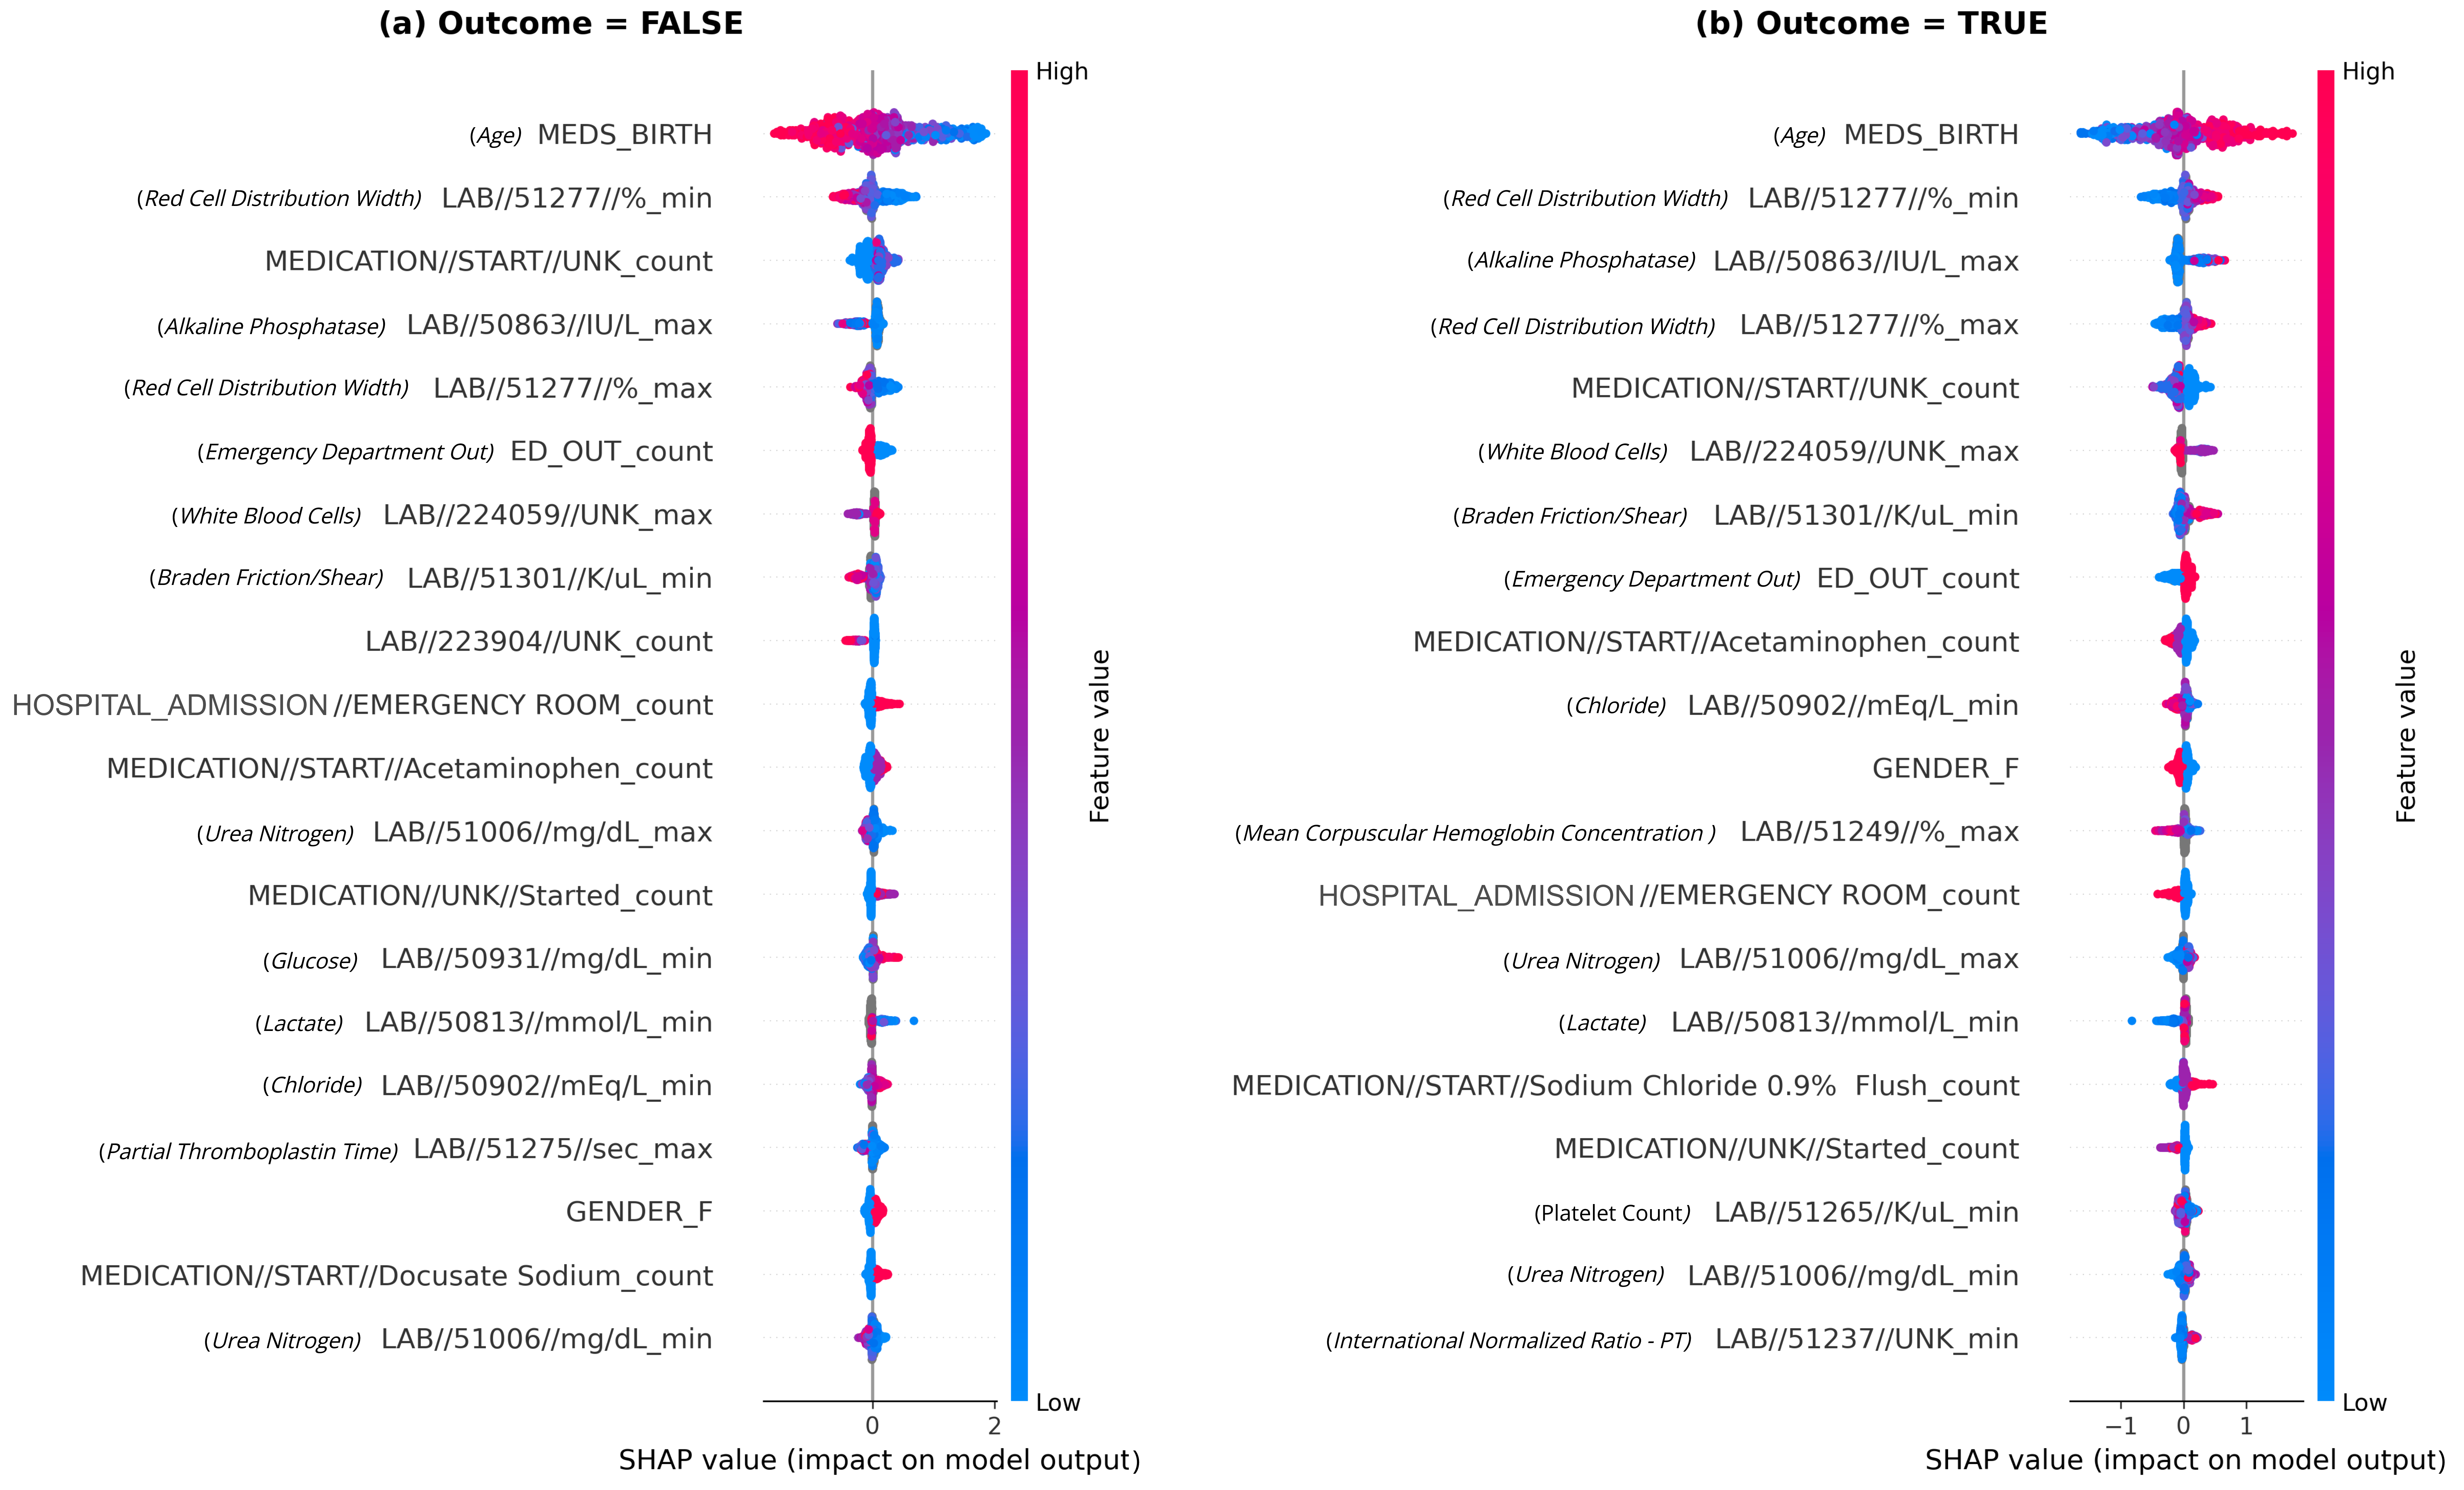
\includegraphics[width=\textwidth]{figures/paper3/fig6.png}
\caption{SHAP summary plots for the XGBoost model used to rank MEDS (code, value) features by importance for SHAP-guided relation pruning on \emph{First 24h in-hospital mortality}, reported separately for each outcome class: (a) FALSE, (b) TRUE. Each point is one patient; horizontal position is the SHAP value (contribution to model output) and colour encodes the feature's value (low to high). For readability, only the top-20 features are shown.}
  \label{fig:paper3_shap-summary}
\end{figure*}

Across MEDS-RDF-Full, varying the retention threshold from the top 1\% to 30\% yielded similar predictive performance (Macro-F1: 0.70--0.72; AUC: 0.77--0.80) while reducing the number of retained relations from 205 to 14; we therefore selected the top 10\% as a balance between graph compactness and predictive performance. At this threshold, MEDS-RDF-Full achieved a Macro-F1 of 0.72 and AUC of 0.80, compared with 0.63 and 0.69 for MEDS-RDF-Partial and 0.56 and 0.59 for MEDS-RDF-Base, respectively. Removing temporal information reduced Macro-F1 to 0.71 and AUC to 0.76, while additionally removing literal information reduced them to 0.70 and 0.75, indicating complementary contributions from temporal and literal information (Table~\ref{tab:paper3_results-ablation}).

\begin{table*}[h]
\caption{Configuration ablation on \emph{First 24h in-hospital mortality}: SHAP-pruning threshold (retained top-percentile of relations by importance), literal/temporal information, and resulting graph size. Experiments use RGCN2+lit with all-MiniLM-L6-v2 for textual values, except \emph{Full (no-time; no-txt)}, where no sentence transformer is used.}
\label{tab:paper3_results-ablation}
\resizebox{\textwidth}{!}{%
\begin{tabular}{llccccccccc}
\hline
\multicolumn{1}{c}{\multirow{2}{*}{Dataset}} & \multicolumn{1}{c}{\multirow{2}{*}{\begin{tabular}[c]{@{}c@{}}MEDS-RDF variant\end{tabular}}} & \multicolumn{1}{l}{\multirow{2}{*}{Predicates}} & \multicolumn{1}{l}{\multirow{2}{*}{Triples}} & \multicolumn{4}{c}{F1-score} & \multirow{2}{*}{Accuracy} & \multirow{2}{*}{AUC} & \multirow{2}{*}{AUPRC} \\ \cline{5-8}
\multicolumn{1}{c}{} & \multicolumn{1}{c}{} & \multicolumn{1}{l}{} & \multicolumn{1}{l}{} & False & True & Macro & Weighted &  &  &  \\ \hline
\multirow{2}{*}{Entire} & Base & 9 & \multirow{2}{*}{2,768,048} & 0.61 ±   0.06 & 0.63 ± 0.12 & 0.62 ± 0.08 & 0.62 ± 0.08 & 0.61 ± 0.06 & 0.66 ± 0.07 & 0.67 ± 0.07 \\
 & Partial & 19 &  & 0.66 ± 0.05 & 0.66 ± 0.06 & 0.66 ± 0.05 & 0.66 ± 0.05 & 0.65 ± 0.04 & 0.73 ± 0.05 & 0.72 ± 0.06 \\
\hline
  Only top 30\% & \multirow{2}{*}{Full} & 205 & \multicolumn{1}{r}{968,738} & 0.70 ± 0.04 & 0.69 ± 0.06 & 0.69 ± 0.05 & 0.69 ± 0.05 & 0.69 ± 0.05 & 0.77 ± 0.04 & 0.78 ± 0.04 \\ 
  Only top 15\% &  & 105 & \multicolumn{1}{r}{511,006} & 0.72 ± 0.05 & 0.71 ± 0.06 & 0.71 ± 0.04 & 0.71 ± 0.04 & 0.71 ± 0.04 & 0.79 ± 0.05 & 0.79 ± 0.05 \\
\hline
\multirow{5}{*}{Only top 10\%} & Base & 7 & \multirow{5}{*}{366,053} & 0.54 ± 0.15 & 0.57 ± 0.16 & 0.56 ± 0.12 & 0.56 ± 0.12 & 0.56 ± 0.06 & 0.59 ± 0.09 & 0.60 ± 0.08 \\
 & Partial & 12 &  & 0.64 ± 0.06 & 0.62 ± 0.05 & 0.63 ± 0.05 & 0.63 ± 0.05 & 0.63 ± 0.05 & 0.69 ± 0.06 & 0.67 ± 0.06 \\
 & Full & 74 &  & \textbf{0.73 ± 0.05} & \textbf{0.71 ± 0.05} & \textbf{0.72 ± 0.04} & \textbf{0.72 ± 0.04} & \textbf{0.72 ± 0.05} & \textbf{0.80 ± 0.05} & \textbf{0.79 ± 0.05} \\
 & \begin{tabular}[c]{@{}l@{}}Full (no-time)\end{tabular} & 74 &  & 0.71 ± 0.05 & 0.71 ± 0.05 & 0.71 ± 0.04 & 0.71 ± 0.04 & 0.70 ± 0.04 & 0.76 ± 0.05 & 0.75 ± 0.05 \\
 & \begin{tabular}[c]{@{}l@{}}Full (no-time;no-txt)\end{tabular} & 74 &  & 0.69 ± 0.05 & 0.70 ± 0.05 & 0.70 ± 0.04 & 0.70 ± 0.04 & 0.69 ± 0.04 & 0.75 ± 0.06 & 0.74 ± 0.06 \\
 \hline
% Only top 30\% & \multirow{4}{*}{Full} & 205 & \multicolumn{1}{r}{968,738} & 0.70 ± 0.04 & 0.69 ± 0.06 & 0.69 ± 0.05 & 0.69 ± 0.05 & 0.69 ± 0.05 & 0.77 ± 0.04 & 0.78 ± 0.04 \\ 
%Only top 15\% &  & 105 & \multicolumn{1}{r}{511,006} & 0.72 ± 0.05 & 0.71 ± 0.06 & 0.71 ± 0.04 & 0.71 ± 0.04 & 0.71 ± 0.04 & 0.79 ± 0.05 & 0.79 ± 0.05 \\
Only top 5\% & \multirow{2}{*}{Full} & 41 & \multicolumn{1}{r}{202,437} & 0.72 ± 0.06 & 0.72 ± 0.06 & 0.72 ± 0.05 & 0.72 ± 0.05 & 0.72 ± 0.06 & 0.80 ± 0.06 & 0.78 ± 0.06 \\
Only top 1\% &  & 14 & \multicolumn{1}{r}{45,892} & 0.71 ± 0.07 & 0.70 ± 0.05 & 0.70 ± 0.05 & 0.70 ± 0.05 & 0.70 ± 0.05 & 0.78 ± 0.05 & 0.76 ± 0.06 \\
\hline
\multicolumn{11}{c}{\textbf{Task : First 24h in-hospital mortality}} \\ \hline
\end{tabular}%
}
\end{table*}
 
\paragraph{Impact of semantic representation across prediction tasks.}\label{sec:paper3_results-schema}
Using the top-10\% SHAP-pruning threshold established in Section~\ref{sec:paper3_results-ablation}, we compared MEDS-RDF-Base, MEDS-RDF-Partial, and MEDS-RDF-Full across the 11 MIMIC-IV prediction tasks. Table~\ref{tab:paper3_results-illustrative} presents three representative tasks, while complete results and comparisons with Logistic Regression, Random Forest, and XGBoost are reported in Supplementary Tables~\ref{tab:paper3_results-schema-full} and~\ref{tab:paper3_results-tabular-full}. Because all pruned variants use the same filtered event set, performance differences isolate the effect of semantic specialization. Macro-F1 increased consistently with schema granularity across all 11 tasks, with MEDS-RDF-Full providing the highest Macro-F1 in every case. %On the unpruned dataset, the same progression was observed in 9 of 11 tasks; the two exceptions disappear once SHAP-guided pruning is applied. This indicate that pruning does not merely make MEDS-RDF-Full tractable, but also removes noise from rare or uninformative codes that can otherwise destabilise the coarser partial schema.
We also evaluated RGCN depth and found no benefit from increasing the number of message-passing layers beyond two: on \emph{First 24 in-hospital mortality}, Macro-F1 decreased from 0.72 with RGCN2+lit to 0.71 with three to five layers, while training time increased from 55.1~$\pm$~29.6~s to 66.4--77.2~s (Suppl. Table~\ref{tab:paper3_rgcn-depth}).
Against tabular baselines, XGBoost achieved the highest mean Macro-F1 across the 11 tasks (0.816), compared with 0.813 for Random Forest and 0.796 for Logistic Regression, while RGCN2+lit with MEDS-RDF-Full (pruned) achieved 0.784. Paired tests identified significant differences between RGCN2+lit and XGBoost in 8 of 11 tasks, with the largest gap for \emph{LOS in ICU $>3$ days} (Macro-F1: 0.831 vs.\ 0.937, $p<0.001$); detailed per-task comparisons are provided in Supplementary Table~\ref{tab:paper3_results-xgb-statistical}.

% \begin{table*}[h]
% \caption{Schema-granularity progression and comparison with the XGBoost tabular baseline for three representative tasks. \emph{Entire} denotes the unpruned dataset; \emph{Only top 10\%} denotes the subset retaining the top 10\% of relations by SHAP importance. \emph{Base}, \emph{Partial}, and \emph{Full} denote the corresponding MEDS-RDF schema variants. The best-performing model--schema combination within each task--dataset block is shown in bold. Full results for all 11 tasks and all tabular baselines are reported in Suppl. Tables \ref{tab:results-schema-full} and \ref{tab:results-tabular-full}.}
% \label{tab:results-illustrative}
% \resizebox{\textwidth}{!}{%
% \begin{tabular}{llllcccccc}
% \hline
% \multicolumn{1}{c}{\multirow{4}{*}{Task}} & \multirow{4}{*}{Model} & \multicolumn{1}{c}{\multirow{4}{*}{Dataset}} & \multicolumn{1}{c}{\multirow{4}{*}{Schema}} & \multicolumn{3}{c}{\multirow{2}{*}{F1-score}} & \multirow{4}{*}{Accuracy} & \multirow{4}{*}{AUC} & \multirow{4}{*}{AUPRC} \\
% \multicolumn{1}{c}{} &  & \multicolumn{1}{c}{} & \multicolumn{1}{c}{} & \multicolumn{3}{c}{} &  &  &  \\ \cline{5-7}
% \multicolumn{1}{c}{} &  & \multicolumn{1}{c}{} & \multicolumn{1}{c}{} & \multirow{2}{*}{False} & \multirow{2}{*}{True} & \multirow{2}{*}{Macro} &  &  &  \\
% \multicolumn{1}{c}{} &  & \multicolumn{1}{c}{} & \multicolumn{1}{c}{} &  &  &  &  &  &  \\ \hline
% \multirow{6}{*}{\begin{tabular}[c]{@{}l@{}}First 24h \\ in-ICU \\ mortality\end{tabular}} & \multicolumn{1}{c}{\multirow{5}{*}{RGCN2+lit}} & \multirow{2}{*}{Entire} & Base & 0.34 ± 0.25 & 0.38 ± 0.22 & 0.36 ± 0.13 & 0.50 ± 0.04 & 0.52 ± 0.07 & 0.53 ± 0.05 \\
%  & \multicolumn{1}{c}{} &  & Partial & 0.60 ± 0.05 & 0.60 ± 0.06 & 0.60 ± 0.05 & 0.59 ± 0.05 & 0.64 ± 0.07 & 0.65 ± 0.06 \\ \cline{3-10} 
%  & \multicolumn{1}{c}{} & \multirow{4}{*}{\begin{tabular}[c]{@{}l@{}}Only \\ top 10\%\end{tabular}} & Base & 0.42 ± 0.23 & 0.31 ± 0.27 & 0.37 ± 0.16 & 0.50 ± 0.02 & 0.50 ± 0.06 & 0.51 ± 0.05 \\
%  & \multicolumn{1}{c}{} &  & Partial & 0.58 ± 0.06 & 0.57 ± 0.13 & 0.58 ± 0.08 & 0.57 ± 0.05 & 0.62 ± 0.06 & 0.62 ± 0.07 \\
%  & \multicolumn{1}{c}{} &  & Full & \textbf{0.74 ± 0.06} & \textbf{0.74 ± 0.05} & \textbf{0.74 ± 0.05} & \textbf{0.74 ± 0.04} & \textbf{0.82 ± 0.05} & \textbf{0.80 ± 0.05} \\
%  & XGBoost &  & Tabular & \textbf{0.78 ± 0.02} & \textbf{0.79 ± 0.02} & \textbf{0.78 ± 0.02} & \textbf{0.78 ± 0.02} & \textbf{0.87 ± 0.02} & \textbf{0.86 ± 0.02} \\ \hline
% \multirow{6}{*}{\begin{tabular}[c]{@{}l@{}}1y post \\ -hospital \\ -discharge \\ mortality\end{tabular}} & \multirow{5}{*}{RGCN2+lit} & \multirow{2}{*}{Entire} & Base & 0.67 ± 0.07 & 0.63 ± 0.15 & 0.65 ± 0.10 & 0.64 ± 0.06 & 0.71 ± 0.06 & 0.70 ± 0.06 \\
%  &  &  & Partial & 0.76 ± 0.06 & 0.73 ± 0.05 & 0.74 ± 0.04 & 0.74 ± 0.04 & 0.82 ± 0.04 & 0.81 ± 0.05 \\ \cline{3-10} 
%  &  & \multirow{4}{*}{\begin{tabular}[c]{@{}l@{}}Only \\ top 10\%\end{tabular}} & Base & 0.63 ± 0.16 & 0.63 ± 0.09 & 0.63 ± 0.11 & 0.61 ± 0.08 & 0.68 ± 0.09 & 0.71 ± 0.06 \\
%  &  &  & Partial & 0.77 ± 0.05 & 0.74 ± 0.05 & 0.76 ± 0.04 & 0.75 ± 0.05 & 0.84 ± 0.04 & 0.83 ± 0.05 \\
%  &  &  & Full & \textbf{0.82 ± 0.05} & \textbf{0.80 ± 0.06} & \textbf{0.81 ± 0.05} & \textbf{0.81 ± 0.05} & \textbf{0.89 ± 0.04} & \textbf{0.89 ± 0.04} \\
%  & XGBoost &  & Tabular & \textbf{0.81 ± 0.01} & \textbf{0.82 ± 0.01} & \textbf{0.82 ± 0.01} & \textbf{0.82 ± 0.01} & \textbf{0.90 ± 0.00} & \textbf{0.90 ± 0.00} \\ \hline
% \multirow{6}{*}{\begin{tabular}[c]{@{}l@{}}Myocardial \\ infarction \\ 1--5Y \\ phenotyping\end{tabular}} & \multirow{5}{*}{RGCN2+lit} & \multirow{2}{*}{Entire} & Base & 0.58 ± 0.09 & 0.55 ± 0.17 & 0.57 ± 0.11 & 0.56 ± 0.05 & 0.62 ± 0.07 & 0.64 ± 0.07 \\
%  &  &  & Partial & 0.70 ± 0.06 & 0.71 ± 0.04 & 0.71 ± 0.04 & 0.70 ± 0.04 & 0.78 ± 0.04 & 0.77 ± 0.05 \\ \cline{3-10} 
%  &  & \multirow{4}{*}{\begin{tabular}[c]{@{}l@{}}Only \\ top 10\%\end{tabular}} & Base & 0.57 ± 0.08 & 0.51 ± 0.21 & 0.54 ± 0.13 & 0.57 ± 0.06 & 0.64 ± 0.06 & 0.66 ± 0.06 \\
%  &  &  & Partial & 0.71 ± 0.05 & 0.71 ± 0.06 & 0.71 ± 0.05 & 0.71 ± 0.05 & 0.78 ± 0.04 & 0.77 ± 0.05 \\
%  &  &  & Full & \textbf{0.72 ± 0.05} & \textbf{0.76 ± 0.06} & \textbf{0.74 ± 0.04} & \textbf{0.73 ± 0.04} & \textbf{0.82 ± 0.04} & \textbf{0.82 ± 0.06} \\
%  & XGBoost &  & Tabular & \textbf{0.74 ± 0.02} & \textbf{0.74 ± 0.02} & \textbf{0.74 ± 0.02} & \textbf{0.74 ± 0.02} & \textbf{0.83 ± 0.02} & \textbf{0.83 ± 0.02} \\ \hline
% \end{tabular}%
% }
% \end{table*}


% Please add the following required packages to your document preamble:
% \usepackage{multirow}
% \usepackage{graphicx}
\begin{table*}[]
\caption{Schema-granularity progression and comparison with the XGBoost tabular baseline for three representative tasks. \emph{Entire} denotes the unpruned dataset; \emph{Only top 10\%} denotes the subset retaining the top 10\% of relations by SHAP importance. \emph{Base}, \emph{Partial}, and \emph{Full} denote the corresponding MEDS-RDF schema variants. The best-performing model--schema combination within each task--dataset block is shown in bold. Full results for all 11 tasks and all tabular baselines are reported in Suppl. Tables \ref{tab:paper3_results-schema-full} and \ref{tab:paper3_results-tabular-full}.}
\label{tab:paper3_results-illustrative}
\resizebox{\textwidth}{!}{%
\begin{tabular}{llllcccccccc}
\hline
\multicolumn{1}{c}{\multirow{2}{*}{Task}} & \multirow{2}{*}{Model} & \multicolumn{1}{c}{\multirow{2}{*}{Dataset}} & \multicolumn{1}{c}{\multirow{2}{*}{Schema}} & \multicolumn{3}{c}{F1-score} & \multirow{2}{*}{Accuracy} & \multirow{2}{*}{AUC} & \multirow{2}{*}{AUPRC} & \multirow{2}{*}{\begin{tabular}[c]{@{}c@{}}Duration\\ (s)\end{tabular}} & \multirow{2}{*}{\begin{tabular}[c]{@{}c@{}}Emission\\ (gCO2eq)\end{tabular}} \\ \cline{5-7}
\multicolumn{1}{c}{} &  & \multicolumn{1}{c}{} & \multicolumn{1}{c}{} & False & True & Macro &  &  &  &  &  \\ \hline
\multirow{6}{*}{\begin{tabular}[c]{@{}l@{}}First 24h \\ in-ICU \\ mortality\end{tabular}} & \multicolumn{1}{c}{\multirow{5}{*}{RGCN2+lit}} & \multirow{2}{*}{Entire} & Base & 0.34 ± 0.25 & 0.38 ± 0.22 & 0.36 ± 0.13 & 0.50 ± 0.04 & 0.52 ± 0.07 & 0.53 ± 0.05 & 23.0 ± 23.6 & 1.78 ± 1.97 \\
 & \multicolumn{1}{c}{} &  & Partial & 0.60 ± 0.05 & 0.60 ± 0.06 & 0.60 ± 0.05 & 0.59 ± 0.05 & 0.64 ± 0.07 & 0.65 ± 0.06 & 131.1 ± 144.1 & 5.47 ± 6.02 \\ \cline{3-12} 
 & \multicolumn{1}{c}{} & \multirow{4}{*}{\begin{tabular}[c]{@{}l@{}}Only \\ top 10\%\end{tabular}} & Base & 0.42 ± 0.23 & 0.31 ± 0.27 & 0.37 ± 0.16 & 0.50 ± 0.02 & 0.50 ± 0.06 & 0.51 ± 0.05 & 5.1 ± 2.5 & 0.21 ± 0.09 \\
 & \multicolumn{1}{c}{} &  & Partial & 0.58 ± 0.06 & 0.57 ± 0.13 & 0.58 ± 0.08 & 0.57 ± 0.05 & 0.62 ± 0.06 & 0.62 ± 0.07 & 14.3 ± 15.8 & 0.57 ± 0.61 \\
 & \multicolumn{1}{c}{} &  & Full & \textbf{0.74 ± 0.06} & \textbf{0.74 ± 0.05} & \textbf{0.74 ± 0.05} & \textbf{0.74 ± 0.04} & \textbf{0.82 ± 0.05} & \textbf{0.80 ± 0.05} & 81.1 ± 36.8 & 3.45 ± 1.57 \\
 & XGBoost &  & Tabular & \textbf{0.78 ± 0.02} & \textbf{0.79 ± 0.02} & \textbf{0.78 ± 0.02} & \textbf{0.78 ± 0.02} & \textbf{0.87 ± 0.02} & \textbf{0.86 ± 0.02} & 2.50 ± 0.19 & 0.07 ± 0.01 \\ \hline
\multirow{6}{*}{\begin{tabular}[c]{@{}l@{}}1y post \\ -hospital \\ -discharge \\ mortality\end{tabular}} & \multirow{5}{*}{RGCN2+lit} & \multirow{2}{*}{Entire} & Base & 0.67 ± 0.07 & 0.63 ± 0.15 & 0.65 ± 0.10 & 0.64 ± 0.06 & 0.71 ± 0.06 & 0.70 ± 0.06 & 42.6 ± 33.6 & 4.19 ± 3.15 \\
 &  &  & Partial & 0.76 ± 0.06 & 0.73 ± 0.05 & 0.74 ± 0.04 & 0.74 ± 0.04 & 0.82 ± 0.04 & 0.81 ± 0.05 & 188.7 ± 152.7 & 8.40 ± 6.87 \\ \cline{3-12} 
 &  & \multirow{4}{*}{\begin{tabular}[c]{@{}l@{}}Only \\ top 10\%\end{tabular}} & Base & 0.63 ± 0.16 & 0.63 ± 0.09 & 0.63 ± 0.11 & 0.61 ± 0.08 & 0.68 ± 0.09 & 0.71 ± 0.06 & 40.5 ± 56.7 & 1.51 ± 2.21 \\
 &  &  & Partial & 0.77 ± 0.05 & 0.74 ± 0.05 & 0.76 ± 0.04 & 0.75 ± 0.05 & 0.84 ± 0.04 & 0.83 ± 0.05 & 39.1 ± 27.5 & 1.57 ± 1.13 \\
 &  &  & Full & \textbf{0.82 ± 0.05} & \textbf{0.80 ± 0.06} & \textbf{0.81 ± 0.05} & \textbf{0.81 ± 0.05} & \textbf{0.89 ± 0.04} & \textbf{0.89 ± 0.04} & 84.5 ± 38.8 & 3.92 ± 1.81 \\
 & XGBoost &  & Tabular & \textbf{0.81 ± 0.01} & \textbf{0.82 ± 0.01} & \textbf{0.82 ± 0.01} & \textbf{0.82 ± 0.01} & \textbf{0.90 ± 0.00} & \textbf{0.90 ± 0.00} & 2.75 ± 0.09 & 0.09 ± 0.01 \\ \hline
\multirow{6}{*}{\begin{tabular}[c]{@{}l@{}}Myocardial \\ infarction \\ 1--5Y \\ phenotyping\end{tabular}} & \multirow{5}{*}{RGCN2+lit} & \multirow{2}{*}{Entire} & Base & 0.58 ± 0.09 & 0.55 ± 0.17 & 0.57 ± 0.11 & 0.56 ± 0.05 & 0.62 ± 0.07 & 0.64 ± 0.07 & 20.5 ± 19.5 & 1.38 ± 1.38 \\
 &  &  & Partial & 0.70 ± 0.06 & 0.71 ± 0.04 & 0.71 ± 0.04 & 0.70 ± 0.04 & 0.78 ± 0.04 & 0.77 ± 0.05 & 50.3 ± 37.1 & 2.12 ± 1.58 \\ \cline{3-12} 
 &  & \multirow{4}{*}{\begin{tabular}[c]{@{}l@{}}Only \\ top 10\%\end{tabular}} & Base & 0.57 ± 0.08 & 0.51 ± 0.21 & 0.54 ± 0.13 & 0.57 ± 0.06 & 0.64 ± 0.06 & 0.66 ± 0.06 & 20.3 ± 26.2 & 0.81 ± 1.02 \\
 &  &  & Partial & 0.71 ± 0.05 & 0.71 ± 0.06 & 0.71 ± 0.05 & 0.71 ± 0.05 & 0.78 ± 0.04 & 0.77 ± 0.05 & 15.9 ± 10.9 & 0.63 ± 0.45 \\
 &  &  & Full & \textbf{0.72 ± 0.05} & \textbf{0.76 ± 0.06} & \textbf{0.74 ± 0.04} & \textbf{0.73 ± 0.04} & \textbf{0.82 ± 0.04} & \textbf{0.82 ± 0.06} & 38.7 ± 25.0 & 1.60 ± 1.11 \\
 & XGBoost &  & Tabular & \textbf{0.74 ± 0.02} & \textbf{0.74 ± 0.02} & \textbf{0.74 ± 0.02} & \textbf{0.74 ± 0.02} & \textbf{0.83 ± 0.02} & \textbf{0.83 ± 0.02} & 2.08 ± 0.16 & 0.05 ± 0.01 \\ \hline
\end{tabular}%
}
\end{table*}


% \subsubsection*{Comparison with tabular baselines}\label{sec:results-tabular}
% Finally, Table~\ref{tab:results-tabular} compares RGCN2+lit on MEDS-RDF-Full (top 10\% of relations by SHAP importance, justified in Section~\ref{sec:results-ablation}) against three tabular baselines (Logistic Regression, Random Forest, XGBoost) on every task; the best-performing model on each task is shown in bold. XGBoost is the strongest tabular model on 8 of 11 tasks, narrowly ahead of Random Forest (mean Macro-F1 across tasks: XGBoost 0.816, Random Forest 0.813, Linear 0.796); on the remaining 3 tasks (\emph{30d re-admission}, \emph{Myocardial Infarction phenotyping}, \emph{CKD onset in diabetics}). %Random Forest is marginally ahead of XGBoost instead, confirming that ``tabular wins'' is a property of tree-based ensembles broadly rather than of XGBoost specifically.
% RGCN2+lit on MEDS-RDF-Full reaches a mean Macro-F1 of 0.784 across the 11 tasks, trailing the best tabular baseline by a moderate margin overall, but the gap is highly task-dependent: RGCN reaches statistical parity with the best tabular baseline on \emph{30d re-admission} (0.70 for RGCN and XGBoost, with Random Forest marginally ahead at 0.71), on \emph{Myocardial Infarction phenotyping} (0.74 for both RGCN and XGBoost, with Random Forest at 0.75), and on \emph{LOS in Hospital $>$3 days} (all models $\approx$0.99, a near-ceiling task). On the \emph{Myocardial Infarction} task in particular, RGCN's True-class F1 (0.76 $\pm$ 0.06) exceeds every tabular model's, including XGBoost's (0.74 $\pm$ 0.02), indicating a more sensitive, if noisier, detector of the positive class despite the tied Macro-F1. The largest remaining gap is on \emph{LOS in ICU $>$3 days} (RGCN 0.83 vs.\ XGBoost 0.94, a 0.11 Macro-F1 gap, the widest of any task) and \emph{CKD onset in diabetics} (0.76 vs.\ 0.81 for both Random Forest and XGBoost); both tasks aggregate many repeated measurements over a comparatively dense window, which may favour tabular count/aggregate features over the relation-typed graph structure. We additionally note that RGCN's standard deviation across folds is consistently 2--4$\times$ larger than the tabular models' (e.g., \emph{LOS in ICU $>$3 days} Macro-F1: RGCN $\pm$0.04 vs.\ XGBoost $\pm$0.01), indicating that graph-based training is less stable across folds than gradient-boosted or linear models, a limitation discussed further in Section~\ref{sec:discussion}.
 
\paragraph{Sustainability.}\label{sec:paper3_results-sustainability}
Building on the schema comparison above, Table~\ref{tab:paper3_results-illustrative} also reports training duration and estimated carbon emission for three representative tasks, while the complete results across all 11 MIMIC-IV tasks are provided in the Suppl. Tables~\ref{tab:paper3_results-sustainability-a}, \ref{tab:paper3_results-sustainability-b}. 
The relationship between pruning and computational cost is more nuanced than schema granularity alone would suggest. Across the 11 tasks, the SHAP-pruned full schema trains faster and emits less CO\textsubscript{2}eq than the unpruned partial schema in 8 tasks. For example, for \emph{1y post-hospital-discharge mortality}, the pruned full schema requires 84.5,s and emits 3.92,gCO\textsubscript{2}eq, compared with 188.7,s and 8.40,gCO\textsubscript{2}eq for the unpruned partial schema, corresponding to a $2.23\times$ reduction in training duration and a 53.3\% reduction in estimated carbon emissions, while also improving Macro-F1 from 0.74 to 0.81. Thus, in this representative case, SHAP-guided pruning makes the more expressive full schema substantially more computationally tractable without sacrificing predictive performance.

\subsection{Discussion}\label{sec:paper3_discussion}
This study demonstrates that MEDS-OWL and \texttt{meds2rdf} provide a faithful, scalable, and extensible RDF representation of MEDS data, while enabling downstream graph-based learning. The following discussion interprets these findings in terms of the conversion pipeline and ontology design, considers the limitations of the current approach, and examines the implications of the predictive results and opportunities for future graph-based learning.

\subsubsection{The MEDS-RDF Conversion Pipeline}
%
\paragraph{Semantic consistency.}
Our semantic evaluation (Section~\ref{sec:paper3_usage-examples}) on the NEUROVASC cohort and the MIMIC-IV demo shows that MEDS-OWL can represent MEDS events and associated provenance in RDF while preserving the intended ontology structure. The resulting graphs were successfully validated with SHACL, supporting semantic and structural consistency of the generated representation. The examples further illustrate that the same ontology and conversion pipeline can be applied across synthetic and real-world MEDS data.

\paragraph{Round-trip fidelity.}
Our round-trip fidelity evaluation (Section~\ref{sec:paper3_fidelity}) shows that MEDS-RDF preserves the core MEDS data model with high fidelity across NEUROVASC, MIMIC-IV, eICU, and NWICU. Structural and subject completeness, as well as fidelity of \texttt{subject\_id}, \texttt{code}, \texttt{time}, and \texttt{numeric\_value}, were 1.0, with zero numeric or temporal error. The only deviations occurred in \texttt{text\_value} and code completeness, reflecting RDF validity constraints on free-text literals and source-code IRIs. \texttt{meds2rdf} handles these cases by normalising invalid text characters and excluding non-conformant codes rather than generating invalid RDF, prioritising semantic validity and queryability over strict byte-level fidelity. Duplicate events sharing the same (\texttt{subject\_id}, \texttt{time}, \texttt{code}) key affect join-based reconstruction but not the RDF representation itself, as MEDS-OWL assigns each event a distinct IRI. This limitation therefore concerns the reconstruction method rather than the ontology.

\paragraph{Scalable conversion.}
The scalability evaluation (Section~\ref{sec:paper3_scalability}) highlights a qualitative difference between the two \texttt{meds2rdf} versions. The v1 converter, based on an in-memory \texttt{rdflib.Graph}, could not complete the three real-world ICU conversions on the 32~GB evaluation machine, whereas v2 successfully converted all four datasets, including MIMIC-IV, which generated a 937~GB plain N-Triples file. The streaming architecture therefore extends \texttt{meds2rdf} to datasets at the scale used in clinical ML research. Gzip compression reduced RDF size by 97--98\% across the evaluated datasets, reducing the MIMIC-IV export from 937~GB to 32~GB at a 27--32\% increase in conversion time (Table~\ref{tab:paper3_scalability}). The \texttt{TripleSink} architecture further supports alternative storage backends without modifying the conversion or mapping logic. As additional MEDS ETL pipelines become available, the same framework can be applied to new MEDS-compliant datasets without changes to the core ontology.

% \paragraph{Semantic consistency}
% Our semantic evaluation on two complementary datasets (Section~\ref{sec:usage-examples}), the synthetic NEUROVASC cohort and a real-world subset of MIMIC-IV, demonstrates that MEDS-OWL can faithfully represent MEDS event data and associated provenance in RDF while remaining compact and operationally pragmatic. The resulting RDF graphs are SHACL-validated, supporting semantic and structural consistency. Moreover, while the neurovasc dataset illustrates a test on a controlled synthetic cohort, the MIMIC-IV conversion demonstrates that the approach scales to large, heterogeneous, real-world data. The latter confirms that \texttt{meds2rdf} can process high event volumes while preserving semantic consistency.

% \paragraph{Round-trip fidelity} 
% Our round-trip fidelity evaluation (Section~\ref{sec:fidelity}) shows that MEDS-RDF preserves the core MEDS data model with high fidelity across NEUROVASC, MIMIC-IV, eICU, and NWICU. Structural and subject completeness, as well as fidelity of \texttt{subject\_id}, \texttt{code}, \texttt{time}, and \texttt{numeric\_value}, were 1.0, with zero numeric or temporal error. The only deviations occurred in \texttt{text\_value} and code completeness, reflecting RDF validity constraints on free-text literals and source-code IRIs; \texttt{meds2rdf} handles these cases by normalising invalid text characters and excluding non-conformant codes rather than producing invalid RDF. This design prioritises semantically valid and queryable graphs over strict byte-level fidelity, while future releases could expose the handling policy as a configurable option. Duplicate events sharing the same (\texttt{subject\_id}, \texttt{time}, \texttt{code}) key also affect join-based reconstruction, but not the RDF representation itself: MEDS-OWL assigns each event a distinct IRI, preserving their identity. This limitation therefore arises from the reconstruction method, motivating future evaluations based on multiset or IRI-aware comparisons.

% \paragraph{Round-trip fidelity}
% Our round-trip fidelity evaluation (Section~\ref{sec:fidelity}) demonstrates that the MEDS-RDF transformation implemented by \texttt{meds2rdf} and MEDS-OWL preserves nearly all tabular field values without loss or distortion. Across four datasets (NEUROVASC, MIMIC-IV, eICU, and NWICU) spanning synthetic and real-world EHR data, structural completeness, subject completeness, and the fidelity of all structured, schema-defined fields, \texttt{subject\_id}, \texttt{code}, \texttt{time}, and \texttt{numeric\_value}, are 1.0, with zero numeric error and zero temporal deviation. These results confirm that the ontology's cardinality constraints and datatype mappings are correctly specified and that \texttt{meds2rdf} implements them faithfully for the core MEDS event model.
 
% The two minor deviations from perfect fidelity reported in Section~\ref{sec:fidelity}, in \texttt{text\_value} and in code completeness, are worth interpreting rather than merely restating. Both originate from the same underlying tension: RDF literal and IRI syntax impose validity constraints (e.g., on permitted characters) that free-form clinical text and locally-coined source codes do not always respect. \texttt{meds2rdf} resolves this tension conservatively, by normalising offending characters in text and by dropping non-conformant codes rather than silently corrupting them or failing the entire conversion. This is a deliberate design trade-off: an alternative implementation could instead escape or percent-encode all non-conformant content to achieve strict byte-for-byte fidelity, at the cost of producing literals and IRIs that are harder to read, query, and reuse downstream. We consider the current behaviour preferable for a library whose primary purpose is to produce semantically meaningful, queryable knowledge graphs rather than an exact binary mirror of the source files, but future releases could expose this as a configurable policy so that users requiring strict fidelity can opt out of normalisation.
 
% The presence of duplicate-key rows, events sharing the same (\texttt{subject\_id}, \texttt{time}, \texttt{code}) composite key, deserves attention. Such rows arise naturally in real-world ICU data, where multiple simultaneous measurements of the same variable are clinically meaningful but cannot be uniquely addressed by a simple join key; their proportions, reported in Section~\ref{sec:fidelity}, are highest in MIMIC-IV. MEDS-OWL handles these correctly by minting a distinct IRI per event, so no information is lost in the RDF graph; the limitation is specific to the join-based reconstruction strategy used in our round-trip evaluation, not to the ontology itself. Future evaluation protocols could address this by adopting multiset comparison or a SPARQL-based reconstruction that exploits the IRI-level identity of events.

% \paragraph{Scalable conversion.}
% The scalability evaluation (Section~\ref{sec:scalability}) reveals a qualitative shift between the two versions of \texttt{meds2rdf}. The v1 converter, built around an in-memory \texttt{rdflib.Graph}, is limited in practice to datasets that fit entirely in RAM. On the 32 GB evaluation machine used in this study, this constraint prevented conversion of all three real-world ICU datasets. The v2 converter, by contrast, completed all four conversions successfully, including MIMIC-IV, which produces a 937 GB plain N-Triples file. This is not merely a quantitative improvement but a qualitative one: the framework transitions from a prototypical research tool to one that can operate on the scale of datasets routinely used in clinical ML research.

% Zip compression substantially reduces storage requirements with a moderate time overhead. Size reductions of 97–98\% across the evaluated datasets (Table~\ref{tab:scalability}) shrink multi-gigabyte, and for MIMIC-IV multi-hundred-gigabyte, N-Triples files to sizes compatible with standard storage quotas and network transfer; for MIMIC-IV specifically, the plain export's 937 GB footprint is reduced to 32 GB. The overhead of compression ranges from 27\% to 32\% of conversion time across all four datasets, a modest cost given the storage savings. For most deployment scenarios, particularly those involving archival, sharing, or ingestion into a triple store via file import, gzip mode is therefore the recommended default.

% The extensible sink architecture, described in Section~\ref{sec:meds2rdf}, further broadens the practical scope of the library. By exposing a stable \texttt{TripleSink} interface, \texttt{meds2rdf} allows users to direct triples to any storage backend, including triple stores such as GraphDB or Virtuoso, cloud object storage, or custom streaming pipelines, without modifying the converter or the mapping logic. This separation of concerns is consistent with the principle of reusability: the conversion layer remains stable while the persistence layer can be adapted to the requirements of each deployment environment.
 
% The choice to evaluate only datasets with pre-existing, publicly available MEDS ETL pipelines is a deliberate methodological decision. It confirms that MEDS-OWL is not tied to a specific institution or data model, but functions as a general semantic layer over any MEDS-compliant dataset. As the MEDS ecosystem grows and additional ETL pipelines are released, the scope of MEDS-OWL applicability will expand correspondingly without requiring changes to the ontology itself.

% \paragraph{Scalable conversion} 
% The scalability evaluation (Section~\ref{sec:scalability}) highlights a qualitative difference between the two \texttt{meds2rdf} versions. The v1 converter, based on an in-memory \texttt{rdflib.Graph}, could not complete the three real-world ICU conversions on the 32~GB evaluation machine, whereas v2 successfully converted all four datasets, including MIMIC-IV, which generated a 937~GB plain N-Triples file. Thus, the streaming architecture extends \texttt{meds2rdf} from a prototype to a tool capable of processing datasets at the scale used in clinical ML research.

% Gzip compression reduced RDF size by 97--98\% across all datasets, reducing the MIMIC-IV export from 937~GB to 32~GB, at a 27--32\% increase in conversion time (Table~\ref{tab:scalability}). This trade-off makes compressed output attractive for storage, transfer, and file-based ingestion. The extensible \texttt{TripleSink} architecture further allows triples to be directed to alternative backends, including triple stores, cloud storage, or custom streaming pipelines, without modifying the conversion or mapping logic.

% As additional MEDS ETL pipelines become available, the same ontology and conversion framework can be applied without requiring changes to the core ontology.

% The evaluation deliberately included only datasets with publicly available MEDS ETL pipelines, providing a reproducible test of MEDS-OWL as a general semantic layer over MEDS-compliant data rather than a framework tied to a specific source dataset. 


\subsubsection{The MEDS-RDF Representation} 
Compared to existing approaches for representing clinical data in RDF including FHIR-RDF, SPHN, and CARE-SM, MEDS-OWL occupies a distinct position. FHIR-RDF provides a direct serialisation of the FHIR resource model but inherits its loosely specified semantics and its clinical-documentation orientation, which is misaligned with the event-centric, ML-oriented design of MEDS. SPHN and CARE-SM demonstrate that patient-centric KG representations can support interoperability and provenance modeling, but they are tightly coupled to specific research infrastructures and semantic frameworks. Moreover, unlike MEDS-RDF's automatically specialized subject-event relations, the others do not offer a built-in mechanism for varying the granularity of the subject-event relation itself. %To the best of our knowledge, no publicly available SPHN-RDF or CARE-SM conversion of MIMIC-IV currently exists. Consequently, a direct, large-scale empirical comparison between these schemas and MEDS-RDF on the MIMIC-IV prediction tasks remains future work.

MEDS-OWL deliberately follows the minimality of MEDS, introducing only the concepts and relations required to represent its data model and reusing established vocabularies such as PROV-O, DCAT, DCTERMS, and SKOS where appropriate. This design limits semantic overhead while preserving the information defined by MEDS, as reflected in the near-complete round-trip fidelity observed across the evaluated datasets. More specialized extensions, including temporal, unit, or richer code ontologies, can therefore be added as optional layers without imposing additional complexity on the core representation.

Exporting MEDS datasets as knowledge graphs also bridges the event-centric, ML-oriented structure of MEDS with the relational expressiveness of graph-based representations. By explicitly encoding entities, relations, and provenance, MEDS-RDF exposes multi-relational dependencies between clinical events that can be directly exploited by graph representation learning methods.


This representation design also has implications for model complexity. The depth-sensitivity analysis (Section~\ref{sec:paper3_results-schema}) showed no measurable predictive benefit from increasing RGCN depth beyond two layers, while computational cost increased. This suggests that the predictive structure encoded by MEDS-RDF can be captured within a relatively local relational neighborhood. Consequently, the semantically explicit but structurally compact representation supports effective prediction with relatively lightweight graph architectures, illustrating that data representation can influence not only semantic expressivity but also the complexity required to exploit it downstream.

% \subsection{Limitations}
% The current evaluation has several limitations that inform the research agenda for future work. First, performance profiling remains incomplete. Conversion times are reported as wall-clock measurements on a single machine configuration and reflect single runs without warm-cache controls. A more rigorous performance analysis would include memory profiling, multi-run averaging, and evaluation across different hardware configurations and triple-store ingestion pipelines. Second, the round-trip evaluation currently covers four datasets. Extending it to additional MEDS-formatted corpora would provide a more comprehensive characterisation of fidelity across the full MEDS data model. Third, SHACL validation statistics across multiple datasets have not yet been systematically aggregated. Running full SHACL validation on the large-scale conversions and reporting violation rates, violation types, and their correlation with data quality issues would strengthen the case for MEDS-OWL as a data quality tool, not only a semantic layer.

% The current MEDS-OWL ontology does not capture certain operational constraints of MEDS datasets. Specifically, MEDS requires subject contiguity, which means that all the features associated with a single subject should appear in a single sort and should be temporally sorted. While temporal ordering becomes largely irrelevant when converting tabular MEDS data to RDF graphs, subject contiguity can be partially represented by associating each subject with a specific ML partition via the meds:SubjectSplit class. Importantly, a single subject may participate in multiple independent splits (e.g., for repeated experiments or cross-validation); however, within each split, the subject can belong to only one subset (e.g., training, validation, or test). This ensures that partitioning is mutually exclusive at the level of each experiment while still supporting multiple, independent splits for variability analysis. To address this limitation, future releases of MEDS-OWL will incorporate enhanced axioms, potentially using disjointness rules or qualified cardinality restrictions in description logics, thereby allowing the ontology to more accurately represent MEDS operational constraints.

\subsubsection{Limitations}
The current evaluation has several limitations. First, performance profiling is limited to wall-clock measurements from single runs on one machine configuration, without warm-cache controls; future analyses should include memory profiling, repeated runs, diverse hardware, and triple-store ingestion. Second, round-trip fidelity was evaluated on four datasets; additional MEDS-formatted corpora would provide broader coverage of the MEDS data model. Third, SHACL validation statistics have not been systematically aggregated across datasets. Full validation of large-scale conversions, including violation rates and types and their relationship to data quality, would further establish MEDS-OWL as a data quality tool in addition to a semantic layer.

MEDS-OWL also does not yet capture all operational constraints of MEDS. In particular, MEDS requires subject contiguity, with all features for a subject appearing in a single sorted sequence. While temporal ordering is largely irrelevant in RDF, subject membership in an ML partition can be represented through the \texttt{meds:SubjectSplit} class. A subject may participate in multiple independent splits, such as repeated experiments or cross-validation, but can belong to only one subset within each split, preserving partition exclusivity while supporting repeated analyses. Future releases will strengthen these constraints through additional axioms, potentially including disjointness rules and qualified cardinality restrictions, to more accurately represent MEDS operational requirements.

\subsubsection{Downstream Predictive Performance}
Section~\ref{sec:paper3_prediction-results} evaluates the downstream value of graph-based representations and the effect of RDF schema design across 11 real MIMIC-IV prediction tasks, using matched, identically seeded cross-validation folds for graph and tabular models. Among the SHAP-pruned variants, which contain the same underlying event set, Macro-F1 increased monotonically from MEDS-RDF-Base to Partial to Full on all 11 tasks, suggesting that predicate specialization is an important determinant of performance in this benchmark. Compared with XGBoost, the strongest tabular baseline overall, RGCN2+lit showed no statistically significant difference on three tasks (\emph{30-day readmission}, \emph{myocardial infarction phenotyping}, and \emph{Hospital LOS}), while XGBoost achieved higher mean Macro-F1 on the remaining eight tasks (Suppl. Table~\ref{tab:paper3_results-xgb-statistical}). Thus, the performance gap was strongly task-dependent, ranging from near-zero on \emph{Hospital LOS} and \emph{30-day readmission} to substantially larger differences on \emph{ICU LOS $>3$ days}.

Three factors may contribute to why MEDS-RDF-Full nevertheless trails XGBoost in mean performance across tasks.

\paragraph{Parameter complexity.} MEDS-RDF-Full introduces many more relation types by assigning a distinct RDF predicate to each retained $(\text{code},\text{value})$ pair. Although basis decomposition limits the growth in RGCN parameters, greater relation granularity still requires estimating more relation-specific coefficients. With a fixed task-specific cohort, this can reduce the amount of supervision available for each relation and make parameter estimation more difficult. This represents a trade-off between semantic expressiveness and statistical efficiency in relation-aware graph models. The threshold analysis in Section~\ref{sec:paper3_results-ablation} suggests that SHAP-guided pruning partly mitigates this trade-off by removing infrequent or low-information relations while retaining most of the predictive signal.

\paragraph{Differences in feature representation.} SHAP-guided pruning is derived from an XGBoost model operating on tabular features that explicitly aggregate clinical events, such as event counts and laboratory-value statistics. The RGCN instead operates directly on the event graph and must recover such aggregate patterns through message passing. Thus, although pruning preserves clinically informative events, the retained event set is optimized for a tabular learner rather than for a graph model. Graph-specific feature-importance methods may therefore provide a more suitable basis for pruning in future work.

\paragraph{Training variability.} The RGCN also shows greater variability across cross-validation folds than the tabular baselines (Suppl. Table~\ref{tab:paper3_results-tabular-full}). This suggests greater sensitivity to the training partition and may contribute to the lower mean performance of the graph model. Such variability is compatible with the stochastic nature of graph neural network training, including parameter initialization and optimization, as well as differences in the graph structure induced by the patients assigned to each fold.


\subsubsection{Future Directions for Graph-Based Learning}
The predictive results suggest that further enriching the graph representation could provide additional opportunities for downstream graph-based learning. Importantly, such enrichment can be performed without modifying the MEDS-OWL ontology definition itself. Because the round-trip fidelity evaluation in Section~\ref{sec:paper3_fidelity} confirms that the RDF representation already preserves all information present in the MEDS source, additional semantics can be layered onto this representation as a post-processing step, working exclusively at the level of generated RDF instances rather than the ontology schema.

The flat \texttt{meds:Code} individuals can be automatically enriched with external ontology hierarchies (e.g., linking ICD-10 or ATC codes to their parent concepts via \texttt{meds:parentCode}, already foreseen in the mapping defined in Suppl. Table \ref{tab:paper3_codes}), providing graph-based models with explicit access to clinical concept hierarchies that are currently only implicit in the code strings. 

Finally, because MEDS events carry an explicit timestamp, the RDF representation also naturally supports the construction of Temporal Knowledge Graphs (TKGs) on top of the existing MEDS-OWL schema, without requiring a dedicated temporal ontology extension. This opens further directions for longitudinal patient modeling and temporally aware prediction tasks, which we plan to investigate jointly with the semantic enrichment and cross-model benchmarking strategies described above.

% \section{Conclusion}\label{sec:conclusion}
% We presented MEDS-OWL, a lightweight ontology that formalizes the MEDS event model using Semantic Web standards, together with \texttt{meds2rdf}, a scalable library for transforming MEDS-compliant datasets into FAIR-aligned MEDS-RDF graphs. The framework preserves MEDS's ML-oriented design while adding explicit semantics, provenance, and links to established biomedical vocabularies, supporting interoperable and reproducible graph-based analysis. The sink-based \texttt{meds2rdf} architecture enabled conversion of four heterogeneous clinical datasets and supported RDF graphs of up to 937~GB, with a 2.7$\times$ speedup over the previous implementation. Round-trip evaluation showed high fidelity for the structured information defined by MEDS, with complete structural and subject preservation. Across 11 MIMIC-IV prediction tasks, increasing semantic granularity from MEDS-RDF-Base to Partial and Full consistently improved Macro-F1 and narrowed the performance gap with tabular baselines, while SHAP-guided pruning made the most expressive representation computationally tractable.
% Overall, these results show that semantic representation extends beyond interoperability and can materially influence the performance and computational characteristics of graph-based clinical ML. MEDS-OWL and \texttt{meds2rdf} therefore provide a practical foundation for interoperable, reproducible, and scalable graph-based analysis of MEDS-formatted clinical data. Future work will evaluate MEDS-RDF against other clinical RDF standards, incorporate external biomedical code hierarchies to further structure the predicate space, and investigate inductive learning settings involving newly introduced patients and event types.

\subsection{Conclusion}\label{sec:paper3_conclusion}
We presented MEDS-OWL, a lightweight ontology that formalizes the MEDS event model using Semantic Web standards, together with \texttt{meds2rdf}, a scalable library for generating FAIR-aligned MEDS-RDF graphs. The framework preserves MEDS's ML-oriented design while adding explicit semantics, provenance, and links to established biomedical vocabularies. Its sink-based architecture enabled conversion of four heterogeneous clinical datasets, including RDF output of up to 937~GB and a 2.7$\times$ speedup over the previous implementation, while round-trip evaluation showed high fidelity with complete structural and subject preservation. Across 11 MIMIC-IV prediction tasks, increasing semantic granularity from MEDS-RDF-Base to Partial and Full consistently improved Macro-F1 and narrowed the gap with tabular baselines; SHAP-guided pruning further enabled the full representation to remain computationally tractable. These findings show that semantic representation can influence not only interoperability but also the predictive and computational properties of graph-based clinical ML. MEDS-OWL and \texttt{meds2rdf} therefore provide a practical foundation for interoperable, reproducible, and scalable analysis of MEDS-formatted clinical data. Future work will compare MEDS-RDF with other clinical RDF standards, incorporate external biomedical code hierarchies, and investigate inductive learning for newly introduced patients and event types.

\subsection*{Reproducibility Statement}
All experiments and dataset conversions presented in this article are fully reproducible using the two repositories described below.
The MEDS-RDF conversion pipeline, together with the round-trip fidelity and scalability evaluations, is available at \url{https://github.com/albertomarfoglia/meds-to-owl-examples}. The outcome prediction experiments on MIMIC-IV leveraging the RGCN+Literals model is available at \href{https://github.com/albertomarfoglia/patient-centric-GNNs}{\texttt{https://github.com/albertomarfoglia/patient- centric-GNNs}}.
They rely only on open-source tools and publicly available data or scripts. All software dependencies and configuration files are specified in the repository, and randomized steps are executed with fixed seeds to ensure repeatability.

\subsection*{Declaration of Generative AI and AI-assisted technologies in the writing process}
During the preparation of this work, the author(s) used ChatGPT model 4.0 in order to proofread some sentences in the manuscript. After using this tool/service, the author(s) reviewed and edited the content as needed and take(s) full responsibility for the content of the publication.

% \printcredits of the source replaced by the CRediT statement built from the source \credit{} commands
\subsection*{CRediT authorship contribution statement}

\textbf{Alberto Marfoglia:} Conceptualization; Methodology; Software; Investigation; Data curation; Writing – review \& editing.
\textbf{Antonella Carbonaro:} Supervision; Writing – review \& editing.
\textbf{Adrien Coulet:} Conceptualization; Supervision; Writing – review \& editing.


\subsection*{Declaration of Competing Interest}
A.C. receives funding from Sanofi and Doctolib companies for research projects independent from this work. The other authors declare that they have no known competing financial interests or personal relationships that could have appeared to influence the work reported in this paper.

\subsection*{Acknowledgements}
This study was partially supported by the Italian Ministry of University and Research under PNRR-PNC Project PNC0000002 “DARE - Digital Lifelong Prevention” (CUP: B53C22006450001) and by the French National Research Agency under the France 2030 program throught the NEUROVASC (ANR-22-PESN-0007) and ShareFAIR(ANR-22-PESN-0008) projects.

% layout: keep the main-text floats before the supplementary material
\FloatBarrier

\subsection{Supplementary Material}
\label{sec:paper3_supplementary}

% Content of papers/meds_owl_JBI_2(1)/supplementary.tex (title page, author block and table of contents of the
% standalone supplementary document omitted; its S-prefixed figure/table numbering is replaced by thesis numbering).

	\subsubsection{Supplementary Figures}
	\label{sec:paper3_supp-figures}
	
	This section provides supplementary figures that give additional detail on the MEDS-OWL ontology, the MEDS-to-RDF conversion workflow, provenance representation, and the graph-learning architecture. These figures support the descriptions and results presented in the main manuscript.
	
	\begin{figure}[ht]
		\centering
		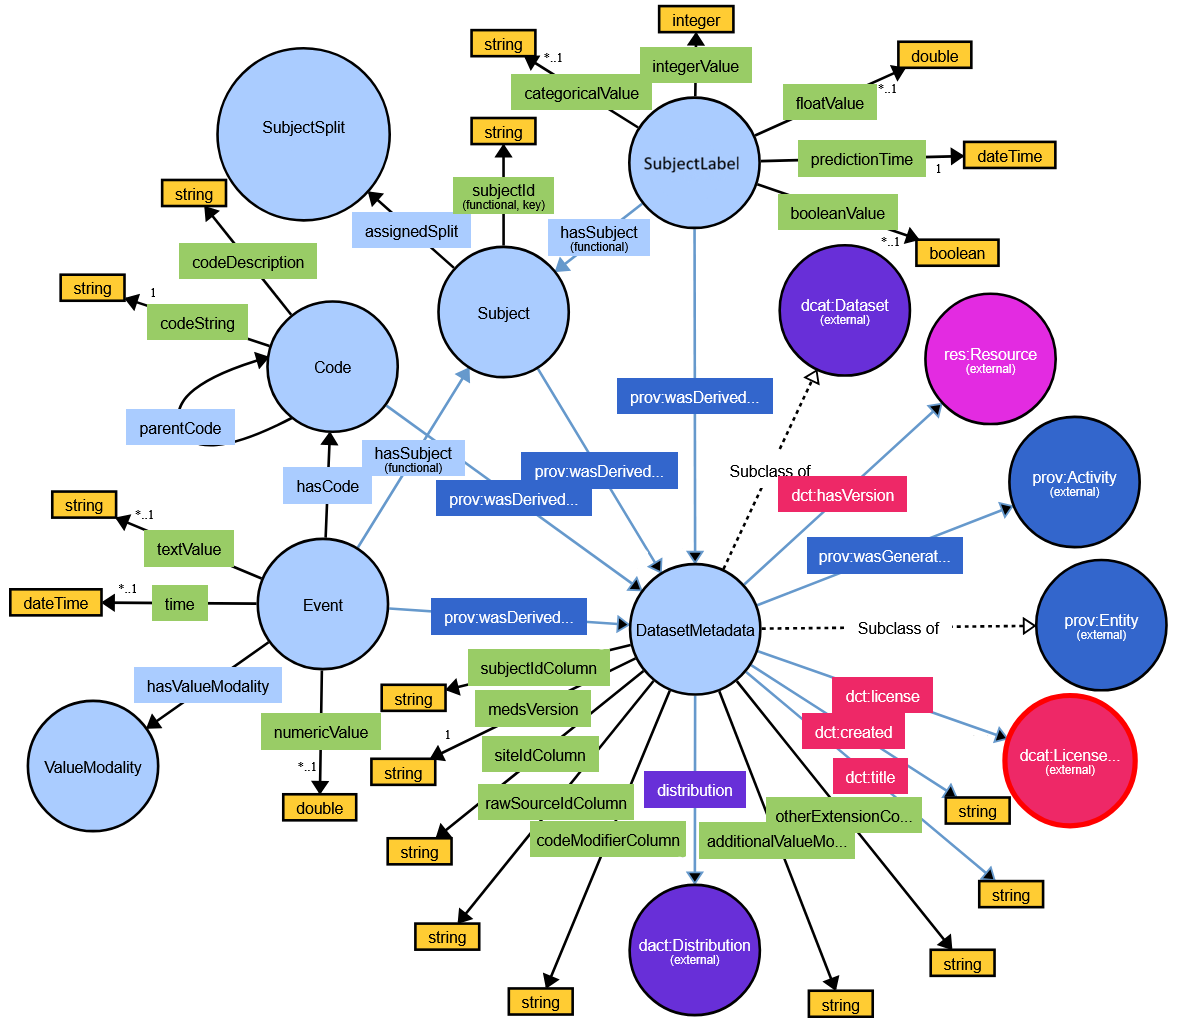
\includegraphics[width=\textwidth]{figures/paper3/fig1.png}
		\caption{Overview of the MEDS-OWL ontology. Azure nodes and edges denote locally defined classes and object properties, respectively. Black edges with green labels are datatype properties. Nodes and edges colored differently indicate imported entities from either the Data Catalogue Vocabulary (\texttt{dcat} prefix), Dublin Core Terms (\texttt{dct} prefix) or PROV-O (prefix \texttt{prov}). Dotted edges represent \texttt{subClassOf} predicate. The figure is drawn with WebVOWL.}%~\citep{lohmann_webvowl_2014}.}
	\label{fig:paper3_ontology-diagram}
\end{figure}

\begin{figure}[ht]
	\centering
	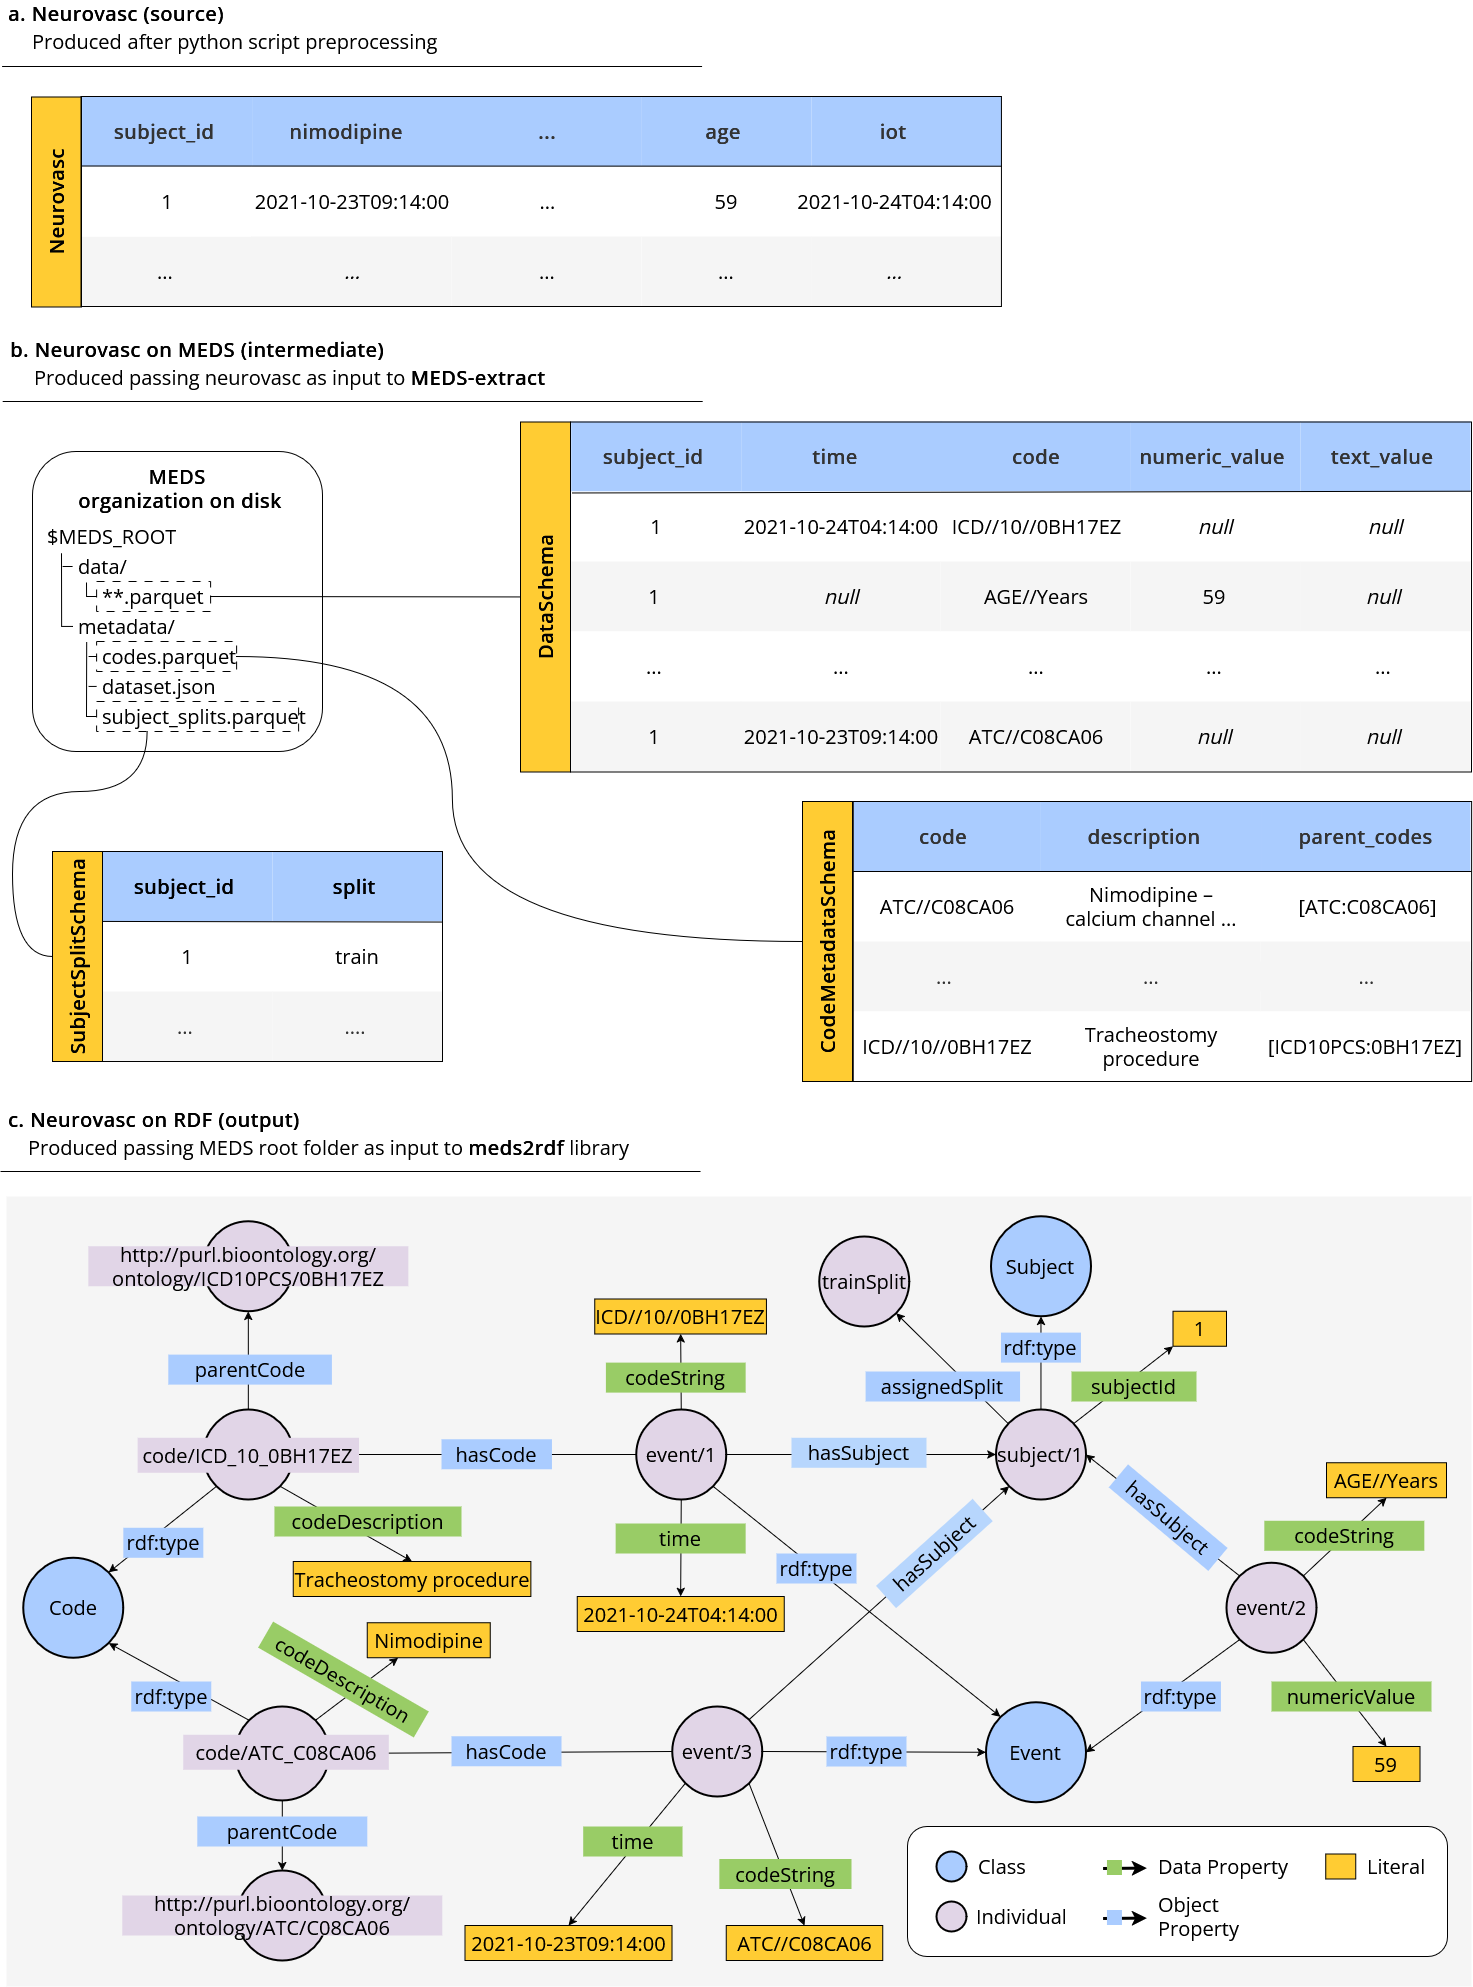
\includegraphics[width=\textwidth]{figures/paper3/fig2.png}
	\caption{MEDS-OWL conversion workflow for the NEUROVASC dataset. (a) Initial preprocessing of three patient features: age, nimodipine administration (ATC code: C08CA06), and tracheostomy procedure (ICD-10-PCS code: 0BH17EZ). (b) Conversion to MEDS tabular format via \texttt{MEDS-extract}, with each feature represented as a distinct event. (c) Transformation of the resulting MEDS dataset into MEDS-RDF using \texttt{meds2rdf}, which instantiates the corresponding MEDS-OWL classes.}
	\label{fig:paper3_etl-conversion}
\end{figure}

\begin{figure}[ht]
	\centering
	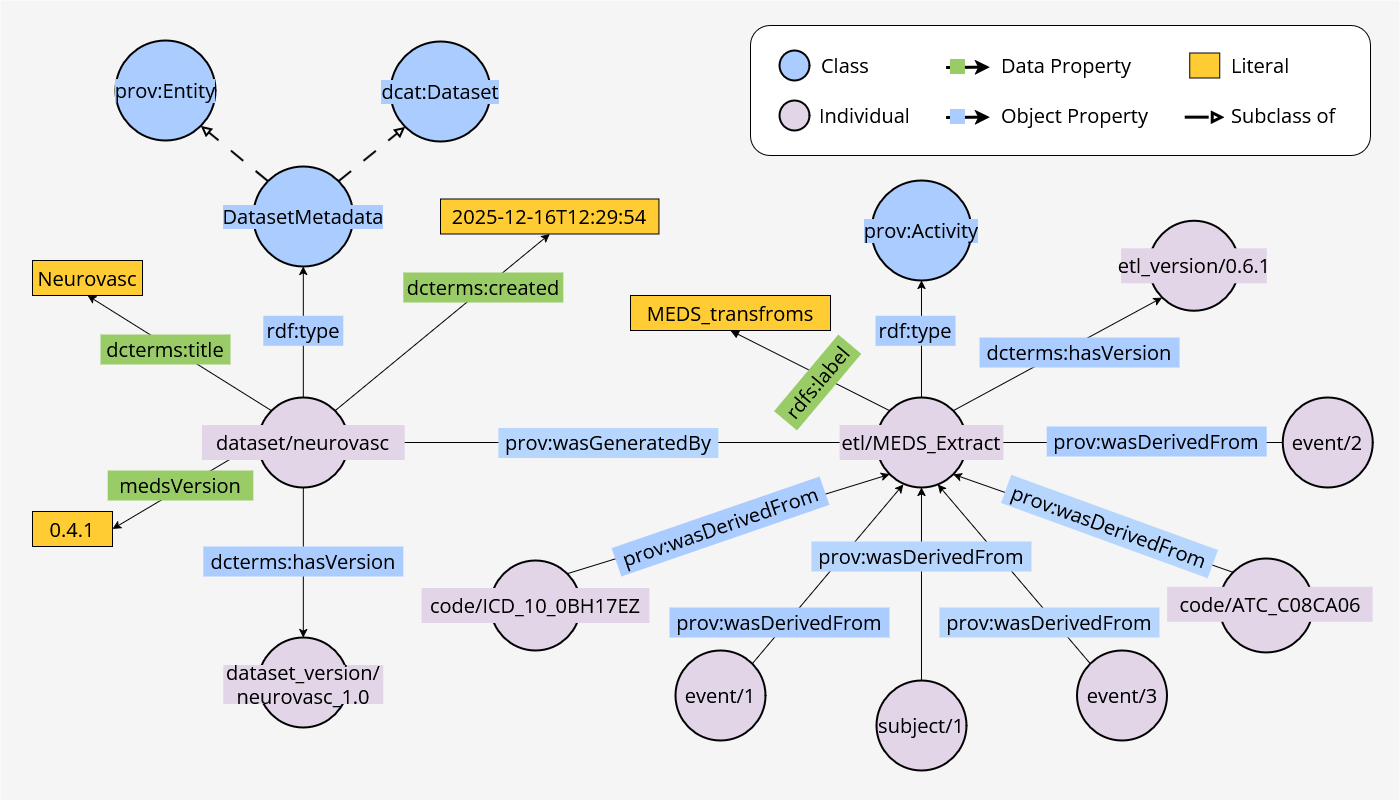
\includegraphics[width=\textwidth]{figures/paper3/fig3.png}
	\caption{Provenance linkage of MEDS events, codes, and subjects using MEDS-OWL, PROV-O, and Dublin Core. Each event references its source \texttt{meds:DatasetMetadata} instance (here, NEUROVASC) via \texttt{prov:wasDerivedFrom}; the dataset metadata records the creation time, MEDS schema version, and dataset title and is associated with the generating ETL activity (\texttt{prov:Activity}), here \texttt{MEDS-extract}.}
	\label{fig:paper3_provenance-instance}
\end{figure}

\begin{figure}[ht]
	\centering
	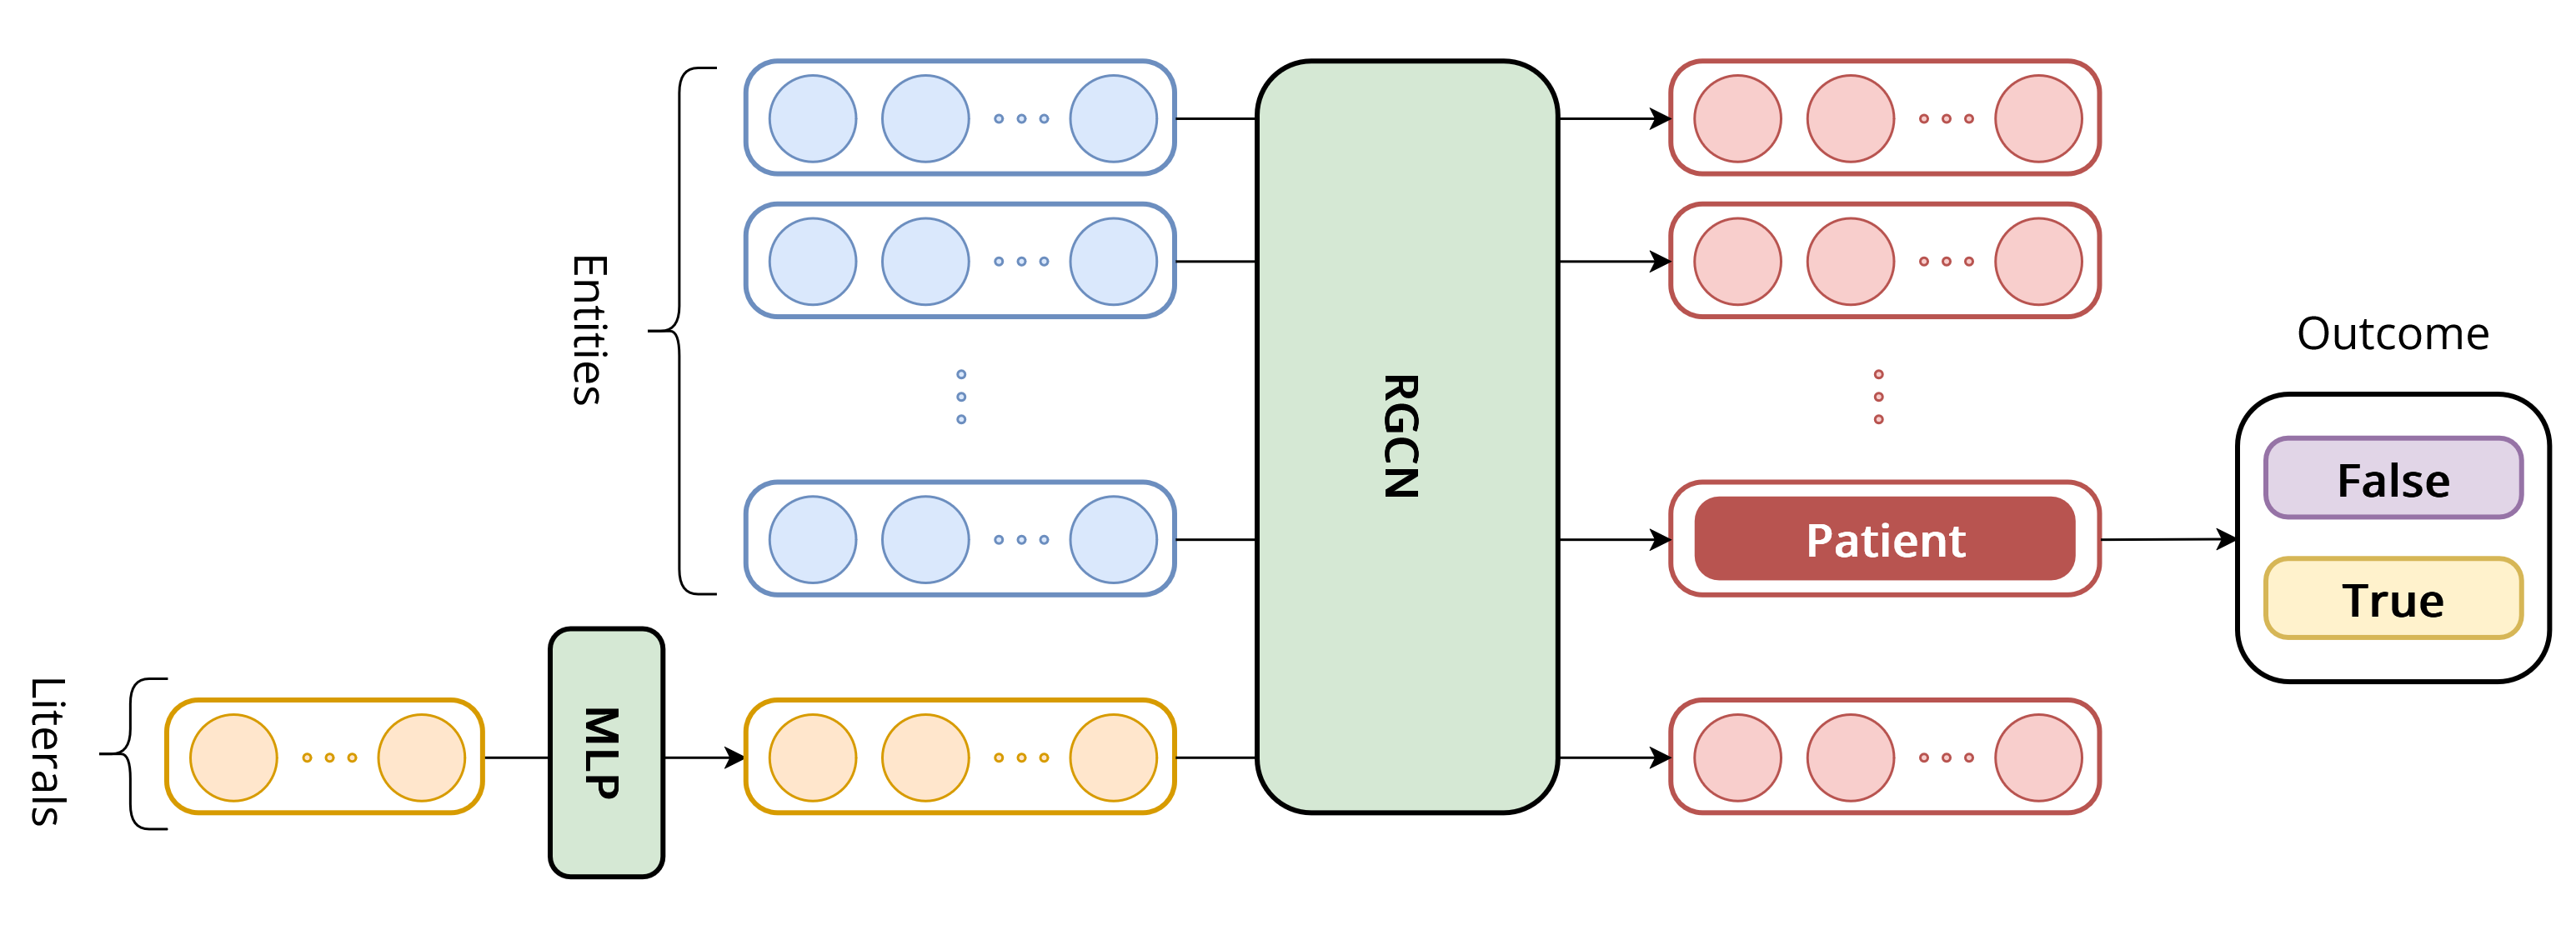
\includegraphics[width=\textwidth]{figures/paper3/fig4.png}
	\caption{Illustration of the RGCN+Lit model for patient outcome prediction.}
	\label{fig:paper3_rcgn+lit}
\end{figure}



%% ============================================================
\subsubsection{MEDS-OWL Mapping Tables}
\label{sec:paper3_supp-mapping-tables}
This section provides supplementary details on the MEDS-OWL ontology and
its correspondence with the MEDS schema. Table~\ref{tab:paper3_meds-owl-concepts}
summarizes the core MEDS-OWL classes, their intended meaning, and
representative examples. Table~\ref{tab:paper3_schema-to-ontology} provides a
high-level correspondence between the main MEDS schema components and the
MEDS-OWL classes used to represent them. The subsequent tables provide the
complete element-level mappings and the corresponding RDF triples:
Table~\ref{tab:paper3_events} details the mapping of the DataSchema elements to
\texttt{meds:Event} and \texttt{meds:Subject}; Table~\ref{tab:paper3_dataset}
details the mapping of DatasetMetadataSchema elements to
\texttt{meds:DatasetMetadata}; Table~\ref{tab:paper3_codes} reports the mapping of
CodeMetadataSchema elements to \texttt{meds:Code}; and
Table~\ref{tab:paper3_labels} reports the mappings of SubjectSplitSchema and
LabelSchema elements to \texttt{meds:SubjectSplit} and
\texttt{meds:SubjectLabel}, respectively.

\begin{table}[ht]
	\centering
	\caption{Core MEDS-OWL classes and their description, as defined by MEDS format.}
	\label{tab:paper3_meds-owl-concepts}
	\begin{tabular}{p{3.3cm} p{6.5cm} p{3.4cm}}
		\hline
		\textbf{Class} & \textbf{Description} & \textbf{Example} \\
		\hline
		\texttt{Subject} &
		Primary entity under observation, typically corresponding to a patient, admission, or longitudinal unit to which events are attributed. &
		Patient \#10234 \\
		\texttt{Event} &
		Atomic clinical observation or intervention representing a single MEDS row, characterized by a subject, a coded concept, and optional temporal and value attributes. &
		Administration of nimodipine at admission \\
		\texttt{Code} &
		An entity used to type events, which includes canonical identifiers, descriptions, and optional linkage to external terminologies or ontologies. &
		ATC:C08CA06 (Nimodipine) \\
		\texttt{DatasetMetadata} &
		Dataset-level description and provenance information, capturing identity, versioning, creation time, and ETL-related metadata. &
		X dataset, in MEDS format, v1.0 \\
		\texttt{SubjectSplit} &
		An assignment  of subjects to several disjoint sets aimed for an ML experiment. &
		Split for experiment 5 into a train, eval, and test sets\\
		\texttt{SubjectLabel} &
		A supervised learning instance defined by a subject identifier, an as-of prediction time (the latest time up to which subject data may be used for the prediction), and exactly one observed ground truth label value \(y\). &
		Subject \#10234, prediction time = discharge date, categorical label = rehabilitation\\
		\texttt{ValueModality} & Generic, extensible entity that links an \texttt{Event} to additional value modalities (for example, images, waveform recordings, audio clips, or other non-tabular payloads). & Chest X-ray image (DICOM series URI)\\
		\hline
	\end{tabular}
\end{table}

\begin{table}[ht]
	\centering
	\caption{Mapping from MEDS schema components to MEDS-OWL classes. See Table~\ref{tab:paper3_meds-owl-concepts} for class definitions and examples.}
	\label{tab:paper3_schema-to-ontology}
	\begin{tabular}{p{2.4cm} p{5.4cm} p{5.4cm}}
		\hline
		\textbf{MEDS schema} & \textbf{Brief description} & \textbf{Mapped MEDS-OWL class(es)} \\
		\hline
		DataSchema &
		Core medical event table describing sequences of subject events, where each row corresponds to a single clinical event. &
		\texttt{meds:Event} as the primary representation of each MEDS row from this table.  
		\texttt{meds:ValueModality} is used to model additional or non-tabular payloads associated with an event (e.g., images, waveforms, signals).  
		See Suppl. Table \ref{tab:paper3_events} for row-to-triple mappings. \\[4pt]%~\ref{tab:events}
		
		DatasetMetadata \\ Schema &
		Dataset-level metadata captures dataset identity, versioning, creation time, licensing, and ETL provenance information. &
		\texttt{meds:DatasetMetadata}, aligned with \texttt{dcterms} and \texttt{dcat}, and linked to ETL activities via \texttt{prov:wasGeneratedBy}.  
		See Suppl. Table \ref{tab:paper3_dataset}. \\[4pt] %~\ref{tab:dataset}
		
		CodeMetadata \\ Schema &
		Metadata describing the controlled vocabularies and codes used to type medical events, including canonical identifiers and hierarchical relations. &
		\texttt{meds:Code}, with \texttt{meds:codeString} as a canonical identifier and optional \texttt{meds:parentCode} relations to represent code hierarchies.  
		See Suppl. Table \ref{tab:paper3_codes}. \\[4pt] %~\ref{tab:codes}
		
		SubjectSplit \\ Schema &
		Specification of how subjects are assigned to disjoint subsets (e.g., for training, tuning, held-out) within a given supervised learning experiment. &
		\texttt{meds:SubjectSplit}, with subjects linked via \texttt{meds:assignedSplit}.  
		Multiple splits may coexist across experiments, while each subject belongs to exactly one subset per split.  
		See Suppl. Table \ref{tab:paper3_labels}. \\[4pt]%~\ref{tab:labels}
		
		LabelSchema &
		Definition of supervised learning labels associated with a subject at a specific prediction time, including the observed ground truth value. &
		\texttt{meds:SubjectLabel}, capturing the prediction cutoff time (\texttt{meds:predictionTime}) and exactly one label value using datatype-specific properties.  
		See Suppl. Table \ref{tab:paper3_labels}. \\[4pt] %~\ref{tab:labels}
		
		(subject identifier) &
		Subject identifiers appear across multiple MEDS schemas and provide the logical join key between events, splits, and labels. &
		\texttt{meds:Subject}, representing the canonical subject entity via \texttt{meds:subjectId}, and serving as the hub linking \texttt{Event}, \texttt{SubjectLabel}, and \texttt{SubjectSplit}. \\
		
		\hline
	\end{tabular}
\end{table}

\begin{table}[ht]
	\centering
	\caption{Mapping of the elements of the MEDS DataSchema tables to \texttt{meds:Event} and \texttt{meds:Subject} classes, with descriptions. For each tuple (or row) of DataSchema, a list of associated RDF triples is generated. Card. stands for the cardinality of the relationship.}
	\label{tab:paper3_events}
	\begin{tabular}{l p{4.8cm} >{\raggedright}p{3.8cm} c}
		\hline
		\textbf{MEDS element} & \textbf{Description} & \textbf{RDF triple} & \textbf{Card.} \\
		\hline
		event\_row e & The row representing an event e of the subject s. & \texttt{?e a meds:Event.}  & 1 \\
		subject\_id id& The identifier of the subject s (typically the patient). & \texttt{?s a meds:Subject. \break ?s meds:subjectId ?id}\verb|^^|\texttt{xsd:string.} \break \texttt{?e meds:hasSubject ?s.} & 1 \\
		time t& The time of the measurement, nullable for static measurements. & \texttt{?e meds:time ?t}\verb|^^|\texttt{xsd:dateTime.} & 0..1 \\
		code c & The categorical descriptor of the measurement (e.g., lab test, diagnosis code). & \texttt{?c a meds:Code. \break ?e meds:hasCode ?c.} & 1 \\
		code\_string cs& The string representation of the code. & \texttt{?e meds:codeString ?cs.}\verb|^^|\texttt{xsd:string.} & 1 \\
		numeric\_value nv & A numeric value associated with the measurement (e.g., lab test result), nullable. & \texttt{?e meds:numericValue ?nv}\verb|^^|\texttt{xsd:double.} & 0..1 \\
		text\_value tv & A text value associated with the measurement (e.g., clinical note, text-based test result), nullable. & \texttt{?e meds:textValue ?tv}\verb|^^|\texttt{xsd:string.} & 0..1 \\
		\hline
	\end{tabular}
\end{table}
%
\begin{table}[ht]
	\centering
	\caption{Mapping metadata of a transformed MEDS dataset (DatasetMetadataSchema) to the \texttt{meds:DatasetMetadata} class. For each dataset generated, a list of associated ``meta'' RDF triples is generated.}
	\label{tab:paper3_dataset}
	\begin{tabular}{l p{3.8cm} >{\raggedright}p{4.6cm} c}
		\hline
		\textbf{MEDS element} & \textbf{Description} & \textbf{RDF triple} & \textbf{Card.} \\
		\hline
		dataset ds & The dataset converted to RDF. & \texttt{?ds a meds:DatasetMetadata.%\break rdfs:subClassOf prov:Entity, dcat:Dataset.
		} & 1 \\
		dataset\_name n & The name of the dataset ds. & \texttt{?ds dct:title ?n}\verb|^^|\texttt{xsd:string.} & 1 \\
		dataset\_version dsv& The version of the dataset. & \texttt{?ds dct:hasVersion ?dsv.} & 0..1 \\
		meds\_version mv& The version of the MEDS schema. & \texttt{?ds meds:medsVersion ?mv}\verb|^^|\texttt{xsd:string.} & 1 \\
		created\_at & ISO 8601 creation date and time. & \texttt{?ds dct:created ?time}\verb|^^|\texttt{xsd:dateTime.} & 1 \\
		license & License under which the dataset is released. & \texttt{?li a dct:LicenseDocument. \break ?ds dct:license ?li.} & 0..1 \\
		location\_uri & URI(s) where the dataset is hosted. & \texttt{?ds dcat:distribution ?dist. \break ?dist dcat:downloadURL ?dw.} & 0..* \\
		description\_uri & URI(s) referencing a detailed description of the dataset. & \texttt{?dist dcat:accessURL ?au.} & 0..* \\
		etl\_name etln& Name of the ETL process etl that generated the dataset. & \texttt{?etl a prov:Activity. \break ?etl rdfs:label ?etln. \break ?ds prov:wasGeneratedBy ?etl.} & 0..1 \\
		etl\_version etlv& Version of the ETL process. & 
		\texttt{?etl dct:hasVersion ?etlv.} & 0..1 \\
		\hline
	\end{tabular}
\end{table}
%
\begin{table}[ht]
	\centering
	\caption{Mapping of the elements of the MEDS CodeMetadataSchema table to \texttt{meds:Code} class. For each tuple (or row) of CodeMetadataSchema, a list of associated RDF triples is generated. } 
	\label{tab:paper3_codes}
	\begin{tabular}{l p{4.2cm} >{\raggedright}p{4.5cm} c}
		\hline
		\textbf{MEDS element} & \textbf{Description} & \textbf{RDF triple} & \textbf{Card.} \\
		\hline
		code\_row c & The row representing a code c in the dataset. & \texttt{?c a meds:Code.} & 1 \\
		code\_string cs & The categorical descriptor of a possible measurement; links to the DataSchema code column. & \texttt{?c meds:codeString ?cs}\verb|^^|\texttt{xsd:string.} & 1 \\
		description d& A human-readable description of what the code represents. & \texttt{?c meds:codeDescription ?d}\verb|^^|\texttt{xsd:string.} & 0..1 \\
		parent\_codes p & One or more higher-level or parent codes in an ontological hierarchy, possibly linking to other codes in MEDS or external vocabularies (e.g., OMOP CDM). & \texttt{?p a meds:Code. \break ?c meds:parentCode ?p.} & 0..* \\
		\hline
	\end{tabular}
\end{table}
%
\begin{table}[ht]
	\centering
	\caption{Mapping of the elements of MEDS SubjectSplitSchema and LabelSchema tables to \texttt{meds:SubjectSplit} and \texttt{meds:SubjectLabel} classes, respectively. For each tuple (or row) of LabelSchema, a list of associated RDF triples is generated.
	}
	\label{tab:paper3_labels}
	\begin{tabular}{l >{\raggedright}p{4.2cm} >{\raggedright}p{4.5cm} c}
		\hline
		\textbf{MEDS element} & \textbf{Description} & \textbf{RDF triple} & \textbf{Card.} \\
		\hline
		split & The name of the subset a subject is assigned to, following a dataset split (e.g., train, validation, test). & \texttt{?set a meds:SubjectSplit. \break ?s a meds:Subject. \break ?s meds:assignedSplit ?set.} & 0..* \\
		
		label\_row & A prediction label (sample) for a subject in a supervised learning task. This is the ground truth label extracted from the dataset according to the task specification. & \texttt{?l a meds:SubjectLabel. \break ?l meds:hasSubject ?s.} & 0..* \\
		
		prediction\_time & The timestamp representing the endpoint of the data that can be used to predict the label for the given sample. This is not necessarily the time of the event itself nor the deployment prediction time. It defines the "as-of" cutoff for input data. & \texttt{?l meds:predictionTime ?pt}\verb|^^|\texttt{xsd:dateTime.} & 1 \\
		
		label\_value & The value for the label. It can be one of the following types depending on the task: binary tasks, ordinal or continuous numeric tasks, and categorical tasks. 
		&
		\texttt{?l meds:booleanValue ?bv}\verb|^^|\texttt{xsd:boolean.} \break
		\texttt{?l meds:integerValue ?iv}\verb|^^|\texttt{xsd:integer.} \break
		\texttt{?l meds:floatValue ?fv}\verb|^^|\texttt{xsd:double.} \break
		\texttt{?l meds:categoricalValue ?cv}\verb|^^|\texttt{xsd:string.} & 0..1 \\
		\hline
	\end{tabular}
\end{table}

%% ============================================================

%\section{Supplementary Methods}

\subsubsection{Round-Trip Fidelity Evaluation}\label{sec:paper3_supp-fidelity}
To assess whether the MEDS-RDF transformation preserves information faithfully, %, beyond the structural statistics reported in Section~\ref{sec:usage-examples},
we conducted a \emph{round-trip fidelity} evaluation across all four datasets previously described. For each dataset, we (\textit{i}) converted a sample of MEDS events to RDF using \texttt{meds2rdf}, (\textit{ii}) reconstructed a tabular representation from the resulting RDF graph, and (\textit{iii}) compared the reconstructed data with the original MEDS source along several dimensions.

\paragraph{Sampling strategy.}
Because several datasets are too large to process exhaustively on a single workstation, we performed $K = 5$ independent random samples per dataset. Each sample $k \in \{1, \ldots, K\}$ was drawn by selecting $N = 100$ patients uniformly at random without replacement, retaining all events associated with those patients. Let $\mathcal{D}_k^{\text{orig}}$ and $\mathcal{D}_k^{\text{recon}}$ denote the sets of events in the original and reconstructed samples, respectively, and let $\mathcal{S}_k^{\text{orig}}$, $\mathcal{S}_k^{\text{recon}}$ denote the corresponding subject sets. For each scalar metric $m$, we report the sample mean $\bar{m} = \frac{1}{K}\sum_{k=1}^{K} m_k$. For the numeric null-rate, where within-dataset variability is clinically meaningful, we additionally report the sample standard deviation $\sigma_m = \sqrt{\frac{1}{K-1}\sum_{k=1}^{K}(m_k - \bar{m})^2}$.

\paragraph{Metrics.}
Let $f \in \{$\texttt{subject\_id}, \texttt{code}, \texttt{time}, \texttt{numeric\_value}, \texttt{text\_value}$\}$ denote a MEDS field, and let $e_i^{\text{orig}}$, $e_i^{\text{recon}}$ denote the values of field $f$ for event $i$ in the original and reconstructed datasets, respectively. We define the following metrics for sample $k$:

\begin{itemize}
	
	\item \emph{Structural completeness}:
	\[
	C_{\text{struct}} = \frac{|\mathcal{D}_k^{\text{recon}}|}{|\mathcal{D}_k^{\text{orig}}|}
	\]
	the proportion of original events successfully recovered after round-trip conversion.
	
	\item \emph{Subject completeness}:
	\[
	C_{\text{subj}} = \frac{|\mathcal{S}_k^{\text{recon}}|}{|\mathcal{S}_k^{\text{orig}}|}
	\]
	the proportion of original subjects whose events appear in the reconstructed dataset.
	
	\item \emph{Field-level fidelity} for field $f$, computed over the $n$ uniquely joinable event pairs:
	\[
	F_f = \frac{1}{n} \sum_{i=1}^{n} \mathbf{1}\!\left[e_i^{\text{recon}} = e_i^{\text{orig}}\right]
	\]
	the exact-match rate. Events with duplicate composite keys $(\texttt{subject\_id}, \texttt{time}, \texttt{code})$ cannot be uniquely matched and are excluded from this metric; their fidelity is assessed separately via approximate matching.
	
	\item \emph{Numeric precision} for \texttt{numeric\_value}, computed over non-null value pairs:
	\[
	\varepsilon_{\max} = \max_i \left| e_i^{\text{recon}} - e_i^{\text{orig}} \right|, \qquad
	\bar{\varepsilon} = \frac{1}{n} \sum_{i=1}^{n} \left| e_i^{\text{recon}} - e_i^{\text{orig}} \right|
	\]
	and the 99th-percentile relative error: \break $\varepsilon_{99} = \operatorname{Quantile}_{0.99}\!\left(\frac{|e_i^{\text{recon}} - e_i^{\text{orig}}|}{|e_i^{\text{orig}}| + \epsilon}\right)$, where $\epsilon = 10^{-9}$ avoids division by zero.
	
	\item \emph{Temporal precision} for \texttt{time}, expressed in seconds:
	\[
	\delta_{\max} = \max_i \left| t_i^{\text{recon}} - t_i^{\text{orig}} \right|_{\text{s}}, \qquad
	\bar{\delta} = \frac{1}{n} \sum_{i=1}^{n} \left| t_i^{\text{recon}} - t_i^{\text{orig}} \right|_{\text{s}}
	\]
	
	\item \emph{Code and split completeness}:
	\[
	C_{\text{code}} = \frac{|\mathcal{C}^{\text{recon}}|}{|\mathcal{C}^{\text{orig}}|}, \qquad
	C_{\text{split}} = \frac{|\mathcal{P}^{\text{recon}}|}{|\mathcal{P}^{\text{orig}}|}
	\]
	where $\mathcal{C}$ and $\mathcal{P}$ denote the sets of distinct codes and split assignments, respectively.
\end{itemize}

\subsubsection{MEDS-RDF Transformation Examples}
\label{sec:paper3_supp-transformation-examples}
% To ground the formal model in practice, we now illustrate the full transformation pipeline from raw clinical data to RDF graphs. We use two datasets, NEUROVASC and MIMIC-IV, chosen to contrast a controlled synthetic cohort with a large-scale real-world EHR dataset.

\paragraph{NEUROVASC example}
The NEUROVASC dataset provides a compact setting for illustrating the full MEDS-RDF pipeline. Each patient is represented by 30 clinical features, including 8 time-stamped events representing the interval from hospital admission to their first occurrence, and 22 non-temporal demographic or historical features. Patient outcomes are categorized in one of three values: Back Home, Rehabilitation, or Death, depending on the patient's status at the end of the hospital stay. %The dataset preserves realistic correlations and event transitions, making it suitable for testing ontology-driven data representation of clinical pathways and basic analytics. 
The complete NEUROVASC transformation workflow is illustrated in Suppl. Figure~\ref{fig:paper3_etl-conversion}, while the corresponding provenance representation is provided in Suppl. Figure~\ref{fig:paper3_provenance-instance}.

The subsequent conversion of MEDS events into RDF using the \texttt{meds2rdf} library results in a KG comprising 1,330,351 RDF triples. The graph contains 255,135 distinct subjects, 18 predicates, and 46,722 distinct objects, corresponding to 255,161 distinct IRIs and 36,594 literals, with no blank nodes generated. In terms of instantiated ontology elements, the graph includes 245,015 individuals of class \texttt{meds:Event}, corresponding one-to-one with the MEDS events, as well as 10,000 \texttt{meds:Subject} instances and 115 \texttt{meds:Code} instances reused across events. Dataset-level metadata is represented by a single \texttt{meds:DatasetMetadata} individual, while three predefined \texttt{meds:SubjectSplit} individuals capture the train, validation, and test partitions. No label instances are generated for this dataset, as outcome labels are not represented in the current transformation.

Finally, we analyzed the structural footprint of events in the resulting RDF graph. Each \texttt{meds:Event} node is described, on average, by 5.31 RDF triples (standard deviation 0.46), with a minimum of 5 and a maximum of 6 triples per event. This low variance reflects the regular structure imposed by MEDS-OWL cardinality constraints, where subject and code associations are mandatory, while temporal and value-related properties are optional. These statistics demonstrate that the transformation produces a compact RDF representation of events while preserving semantic richness and provenance information.

\paragraph{MIMIC-IV example of usage} To further demonstrate the applicability of \texttt{meds2rdf} to real-world EHRs at a level of detail comparable to the NEUROVASC example above, we applied the library to the publicly available \textit{MIMIC-IV demo} dataset, a fixed, pre-defined 100-patient subset of MIMIC-IV already formatted in MEDS. We use this small, openly accessible demo specifically for this illustrative example, as it keeps the workflow tractable for visualization and reproducibility. %The round-trip fidelity and scalability evaluations reported in Sections~\ref{sec:fidelity} and \ref{sec:scalability} instead use the full MIMIC-IV dataset, and are therefore not directly comparable to the statistics reported below.

The conversion generated 916,166 MEDS events distributed across the ML splits as follows: 803,992 in the train set, 69,620 in the tuning set, and 42,554 in the held-out set. The resulting KG comprises 6,408,529 RDF triples, including 925,706 distinct subjects, 19 predicates, 126,680 distinct objects, 925,733 distinct IRIs, and 117,132 literals, with no blank nodes generated. Ontology instantiation includes 916,166 individuals of class \texttt{meds:Event}, 100 \texttt{meds:Subject} individuals, 9,435 \texttt{meds:Code} individuals, three \texttt{meds:SubjectSplit} individuals, and one \texttt{meds:DatasetMetadata} individual. No label or \texttt{ValueModality} instances were included in this subset. Each \texttt{meds:Event} in the MIMIC-IV subset is represented by an average of 6.97 RDF triples (median 7.0, minimum 5, maximum 8, standard deviation 0.42), indicating a slightly richer structure per event compared to NEUROVASC, due to the higher number of numeric and text values associated with MIMIC events. As with the NEUROVASC example, this conversion used the \texttt{GraphSink} strategy. %Together, these two usage examples confirm that \texttt{meds2rdf} preserves the semantic and provenance structure defined by MEDS-OWL; the next two subsections evaluate this preservation, and the computational cost of achieving it, systematically and at scale across all four datasets.

\subsubsection{Full Prediction Task Results}
\label{sec:paper3_supp-results}

This section reports the complete per-task results. Table~\ref{tab:paper3_results-schema-full} reports the full schema-granularity progression (MEDS-RDF-Base, -Partial, and -Full) across all 11 MIMIC-IV prediction tasks, considering both the entire (unpruned) dataset and the SHAP-pruned subset. Table~\ref{tab:paper3_rgcn-depth} reports the sensitivity of predictive performance and computational cost to increasing the RGCN depth from two to five layers. Table~\ref{tab:paper3_results-tabular-full} reports the complete comparison of RGCN2+lit (MEDS-RDF-Full, SHAP-pruned) with the three tabular baselines (Logistic Regression, Random Forest, and XGBoost) across all 11 tasks. Finally, Table~\ref{tab:paper3_results-xgb-statistical} provides the subsample-level Macro-F1 results for RGCN+lit and XGBoost, together with the paired differences and statistical significance of their performance differences across the five patient subsamples for each task.

% Please add the following required packages to your document preamble:
% \usepackage{multirow}
% \usepackage{graphicx}
\begin{table}[ht]
	\caption{Schema-granularity progression across MIMIC-IV tasks. \emph{Entire} denotes the unpruned dataset; \emph{Only top 10\%} denotes the subset retaining the top 10\% of relations by SHAP importance. \emph{Base}, \emph{Partial}, and \emph{Full} denote the corresponding MEDS-RDF schema variants. The winning schema per task is shown in bold.}
	\label{tab:paper3_results-schema-full}
	\resizebox{\textwidth}{!}{%
		\begin{tabular}{lllcccccc}
			\hline
			\multicolumn{1}{c}{\multirow{4}{*}{Task}} & \multicolumn{1}{c}{\multirow{4}{*}{Dataset}} & \multicolumn{1}{c}{\multirow{4}{*}{\begin{tabular}[c]{@{}c@{}}Schema\end{tabular}}} & \multicolumn{3}{c}{\multirow{2}{*}{F1-score}} & \multirow{4}{*}{Accuracy} & \multirow{4}{*}{AUC} & \multirow{4}{*}{AUPRC} \\
			\multicolumn{1}{c}{} & \multicolumn{1}{c}{} & \multicolumn{1}{c}{} & \multicolumn{3}{c}{} &  &  &  \\ \cline{4-6}
			\multicolumn{1}{c}{} & \multicolumn{1}{c}{} & \multicolumn{1}{c}{} & \multirow{2}{*}{False} & \multirow{2}{*}{True} & \multirow{2}{*}{Macro} &  &  &  \\
			\multicolumn{1}{c}{} & \multicolumn{1}{c}{} & \multicolumn{1}{c}{} &  &  &  &  &  &  \\ \hline
			\multirow{5}{*}{\begin{tabular}[c]{@{}l@{}}First 24h \\ in-hospital\\ mortality\end{tabular}} & \multirow{2}{*}{Entire} & Base & 0.61 ± 0.06 & 0.63 ± 0.12 & 0.62 ± 0.08 & 0.61 ± 0.06 & 0.66 ± 0.07 & 0.67 ± 0.07 \\
			&  & Partial & 0.66 ± 0.05 & 0.66 ± 0.06 & 0.66 ± 0.05 & 0.65 ± 0.04 & 0.73 ± 0.05 & 0.72 ± 0.06 \\ \cline{2-9} 
			& \multirow{3}{*}{\begin{tabular}[c]{@{}l@{}}Only \\ top 10\%\end{tabular}} & Base & 0.54 ± 0.15 & 0.57 ± 0.16 & 0.56 ± 0.12 & 0.56 ± 0.06 & 0.59 ± 0.09 & 0.60 ± 0.08 \\
			&  & Partial & 0.64 ± 0.06 & 0.62 ± 0.05 & 0.63 ± 0.05 & 0.63 ± 0.05 & 0.69 ± 0.06 & 0.67 ± 0.06 \\
			&  & Full & \textbf{0.73 ± 0.05} & \textbf{0.71 ± 0.05} & \textbf{0.72 ± 0.04} & \textbf{0.72 ± 0.05} & \textbf{0.80 ± 0.05} & \textbf{0.79 ± 0.05} \\ \hline
			\multirow{5}{*}{\begin{tabular}[c]{@{}l@{}}First 24h \\ in-ICU\\ mortality\end{tabular}} & \multirow{2}{*}{Entire} & Base & 0.34 ± 0.25 & 0.38 ± 0.22 & 0.36 ± 0.13 & 0.50 ± 0.04 & 0.52 ± 0.07 & 0.53 ± 0.05 \\
			&  & Partial & 0.60 ± 0.05 & 0.60 ± 0.06 & 0.60 ± 0.05 & 0.59 ± 0.05 & 0.64 ± 0.07 & 0.65 ± 0.06 \\ \cline{2-9} 
			& \multirow{3}{*}{\begin{tabular}[c]{@{}l@{}}Only \\ top 10\%\end{tabular}} & Base & 0.42 ± 0.23 & 0.31 ± 0.27 & 0.37 ± 0.16 & 0.50 ± 0.02 & 0.50 ± 0.06 & 0.51 ± 0.05 \\
			&  & Partial & 0.58 ± 0.06 & 0.57 ± 0.13 & 0.58 ± 0.08 & 0.57 ± 0.05 & 0.62 ± 0.06 & 0.62 ± 0.07 \\
			&  & Full & \textbf{0.74 ± 0.06} & \textbf{0.74 ± 0.05} & \textbf{0.74 ± 0.05} & \textbf{0.74 ± 0.04} & \textbf{0.82 ± 0.05} & \textbf{0.80 ± 0.05} \\ \hline
			\multirow{5}{*}{\begin{tabular}[c]{@{}l@{}}First 48h \\ in-hospital\\ mortality\end{tabular}} & \multirow{2}{*}{Entire} & Base & 0.45 ± 0.22 & 0.50 ± 0.20 & 0.48 ± 0.16 & 0.53 ± 0.06 & 0.55 ± 0.08 & 0.58 ± 0.07 \\
			&  & Partial & 0.67 ± 0.06 & 0.67 ± 0.06 & 0.67 ± 0.05 & 0.66 ± 0.05 & 0.72 ± 0.06 & 0.71 ± 0.07 \\ \cline{2-9} 
			& \multirow{3}{*}{\begin{tabular}[c]{@{}l@{}}Only \\ top 10\%\end{tabular}} & Base & 0.55 ± 0.20 & 0.46 ± 0.23 & 0.51 ± 0.17 & 0.55 ± 0.06 & 0.57 ± 0.10 & 0.58 ± 0.08 \\
			&  & Partial & 0.65 ± 0.05 & 0.64 ± 0.06 & 0.65 ± 0.04 & 0.64 ± 0.04 & 0.70 ± 0.05 & 0.70 ± 0.06 \\
			&  & Full & \textbf{0.74 ± 0.06} & \textbf{0.72 ± 0.06} & \textbf{0.73 ± 0.05} & \textbf{0.73 ± 0.05} & \textbf{0.80 ± 0.05} & \textbf{0.79 ± 0.07} \\ \hline
			\multirow{5}{*}{\begin{tabular}[c]{@{}l@{}}First 48h \\ in-ICU\\ mortality\end{tabular}} & \multirow{2}{*}{Entire} & Base & 0.45 ± 0.19 & 0.49 ± 0.32 & 0.47 ± 0.19 & 0.52 ± 0.03 & 0.52 ± 0.06 & 0.54 ± 0.05 \\
			&  & Partial & 0.62 ± 0.05 & 0.63 ± 0.06 & 0.63 ± 0.04 & 0.62 ± 0.04 & 0.66 ± 0.05 & 0.66 ± 0.05 \\ \cline{2-9} 
			& \multirow{3}{*}{\begin{tabular}[c]{@{}l@{}}Only \\ top 10\%\end{tabular}} & Base & 0.44 ± 0.27 & 0.57 ± 0.22 & 0.51 ± 0.19 & 0.56 ± 0.08 & 0.57 ± 0.10 & 0.58 ± 0.09 \\
			&  & Partial & 0.61 ± 0.08 & 0.61 ± 0.07 & 0.61 ± 0.06 & 0.60 ± 0.05 & 0.65 ± 0.06 & 0.66 ± 0.06 \\
			&  & Full & \textbf{0.74 ± 0.05} & \textbf{0.74 ± 0.06} & \textbf{0.74 ± 0.05} & \textbf{0.74 ± 0.05} & \textbf{0.82 ± 0.05} & \textbf{0.81 ± 0.06} \\ \hline
			\multirow{5}{*}{\begin{tabular}[c]{@{}l@{}}LOS in ICU \\ \textgreater 3 days\end{tabular}} & \multirow{2}{*}{Entire} & Base & 0.72 ± 0.13 & 0.79 ± 0.14 & 0.76 ± 0.12 & 0.76 ± 0.07 & 0.84 ± 0.06 & 0.86 ± 0.06 \\
			&  & Partial & 0.59 ± 0.08 & 0.59 ± 0.10 & 0.59 ± 0.09 & 0.59 ± 0.08 & 0.62 ± 0.11 & 0.63 ± 0.10 \\ \cline{2-9} 
			& \multirow{3}{*}{\begin{tabular}[c]{@{}l@{}}Only \\ top 10\%\end{tabular}} & Base & 0.58 ± 0.29 & 0.70 ± 0.25 & 0.64 ± 0.24 & 0.69 ± 0.14 & 0.74 ± 0.16 & 0.77 ± 0.16 \\
			&  & Partial & 0.68 ± 0.08 & 0.67 ± 0.10 & 0.68 ± 0.08 & 0.67 ± 0.09 & 0.73 ± 0.09 & 0.73 ± 0.09 \\
			&  & Full & \textbf{0.83 ± 0.04} & \textbf{0.83 ± 0.05} & \textbf{0.83 ± 0.04} & \textbf{0.83 ± 0.04} & \textbf{0.91 ± 0.03} & \textbf{0.91 ± 0.03} \\ \hline
			\multirow{5}{*}{\begin{tabular}[c]{@{}l@{}}LOS \\ in Hospital \\ \textgreater 3 days\end{tabular}} & \multirow{2}{*}{Entire} & Base & 0.73 ± 0.05 & 0.81 ± 0.05 & 0.77 ± 0.04 & 0.76 ± 0.04 & 0.84 ± 0.04 & 0.85 ± 0.04 \\
			&  & Partial & 0.99 ± 0.01 & 0.99 ± 0.01 & 0.99 ± 0.01 & 0.99 ± 0.01 & 0.99 ± 0.01 & 1.00 ± 0.01 \\ \cline{2-9} 
			& \multirow{3}{*}{\begin{tabular}[c]{@{}l@{}}Only \\ top 10\%\end{tabular}} & Base & 0.72 ± 0.06 & 0.82 ± 0.06 & 0.77 ± 0.04 & 0.75 ± 0.05 & 0.84 ± 0.04 & 0.85 ± 0.05 \\
			&  & Partial & 0.99 ± 0.01 & 0.99 ± 0.02 & 0.99 ± 0.01 & 0.99 ± 0.01 & 1.00 ± 0.01 & 1.00 ± 0.00 \\
			&  & Full & \textbf{0.99 ± 0.01} & \textbf{1.00 ± 0.01} & \textbf{0.99 ± 0.01} & \textbf{0.99 ± 0.01} & \textbf{1.00 ± 0.01} & \textbf{1.00 ± 0.00} \\ \hline
			\multirow{5}{*}{\begin{tabular}[c]{@{}l@{}}1y \\ post-hospital- \\discharge \\ mortality\end{tabular}} & \multirow{2}{*}{Entire} & Base & 0.67 ± 0.07 & 0.63 ± 0.15 & 0.65 ± 0.10 & 0.64 ± 0.06 & 0.71 ± 0.06 & 0.70 ± 0.06 \\
			&  & Partial & 0.76 ± 0.06 & 0.73 ± 0.05 & 0.74 ± 0.04 & 0.74 ± 0.04 & 0.82 ± 0.04 & 0.81 ± 0.05 \\ \cline{2-9} 
			& \multirow{3}{*}{\begin{tabular}[c]{@{}l@{}}Only \\ top 10\%\end{tabular}} & Base & 0.63 ± 0.16 & 0.63 ± 0.09 & 0.63 ± 0.11 & 0.61 ± 0.08 & 0.68 ± 0.09 & 0.71 ± 0.06 \\
			&  & Partial & 0.77 ± 0.05 & 0.74 ± 0.05 & 0.76 ± 0.04 & 0.75 ± 0.05 & 0.84 ± 0.04 & 0.83 ± 0.05 \\
			&  & Full & \textbf{0.82 ± 0.05} & \textbf{0.80 ± 0.06} & \textbf{0.81 ± 0.05} & \textbf{0.81 ± 0.05} & \textbf{0.89 ± 0.04} & \textbf{0.89 ± 0.04} \\ \hline
			\multirow{5}{*}{\begin{tabular}[c]{@{}l@{}}30d \\ post-hospital- \\discharge \\ mortality\end{tabular}} & \multirow{2}{*}{Entire} & Base & 0.75 ± 0.06 & 0.71 ± 0.06 & 0.73 ± 0.04 & 0.72 ± 0.05 & 0.79 ± 0.04 & 0.79 ± 0.06 \\
			&  & Partial & 0.79 ± 0.06 & 0.76 ± 0.04 & 0.77 ± 0.04 & 0.77 ± 0.04 & 0.85 ± 0.03 & 0.84 ± 0.04 \\ \cline{2-9} 
			& \multirow{3}{*}{\begin{tabular}[c]{@{}l@{}}Only \\ top 10\%\end{tabular}} & Base & 0.69 ± 0.12 & 0.73 ± 0.07 & 0.71 ± 0.09 & 0.71 ± 0.06 & 0.78 ± 0.10 & 0.79 ± 0.08 \\
			&  & Partial & 0.79 ± 0.06 & 0.78 ± 0.05 & 0.79 ± 0.04 & 0.79 ± 0.04 & 0.87 ± 0.04 & 0.86 ± 0.04 \\
			&  & Full & \textbf{0.87 ± 0.04} & \textbf{0.86 ± 0.04} & \textbf{0.86 ± 0.03} & \textbf{0.86 ± 0.03} & \textbf{0.94 ± 0.02} & \textbf{0.94 ± 0.02} \\ \hline
			\multirow{5}{*}{\begin{tabular}[c]{@{}l@{}}30d \\ re-admission\end{tabular}} & \multirow{2}{*}{Entire} & Base & 0.64 ± 0.09 & 0.61 ± 0.17 & 0.62 ± 0.10 & 0.60 ± 0.06 & 0.65 ± 0.07 & 0.65 ± 0.07 \\
			&  & Partial & 0.58 ± 0.05 & 0.61 ± 0.07 & 0.59 ± 0.06 & 0.59 ± 0.06 & 0.63 ± 0.05 & 0.65 ± 0.06 \\ \cline{2-9} 
			& \multirow{3}{*}{\begin{tabular}[c]{@{}l@{}}Only \\ top 10\%\end{tabular}} & Base & 0.63 ± 0.06 & 0.61 ± 0.15 & 0.62 ± 0.09 & 0.62 ± 0.05 & 0.68 ± 0.04 & 0.69 ± 0.05 \\
			&  & Partial & 0.62 ± 0.05 & 0.66 ± 0.08 & 0.64 ± 0.06 & 0.64 ± 0.06 & 0.69 ± 0.06 & 0.69 ± 0.06 \\
			&  & Full & \textbf{0.68 ± 0.05} & \textbf{0.72 ± 0.06} & \textbf{0.70 ± 0.05} & \textbf{0.70 ± 0.05} & \textbf{0.76 ± 0.05} & \textbf{0.78 ± 0.05} \\ \hline
			\multirow{5}{*}{\begin{tabular}[c]{@{}l@{}}Myocardial \\ infarction\\ 1--5Y \\ phenotyping\end{tabular}} & \multirow{2}{*}{Entire} & Base & 0.58 ± 0.09 & 0.55 ± 0.17 & 0.57 ± 0.11 & 0.56 ± 0.05 & 0.62 ± 0.07 & 0.64 ± 0.07 \\
			&  & Partial & 0.70 ± 0.06 & 0.71 ± 0.04 & 0.71 ± 0.04 & 0.70 ± 0.04 & 0.78 ± 0.04 & 0.77 ± 0.05 \\ \cline{2-9} 
			& \multirow{3}{*}{\begin{tabular}[c]{@{}l@{}}Only \\ top 10\%\end{tabular}} & Base & 0.57 ± 0.08 & 0.51 ± 0.21 & 0.54 ± 0.13 & 0.57 ± 0.06 & 0.64 ± 0.06 & 0.66 ± 0.06 \\
			&  & Partial & 0.71 ± 0.05 & 0.71 ± 0.06 & 0.71 ± 0.05 & 0.71 ± 0.05 & 0.78 ± 0.04 & 0.77 ± 0.05 \\
			&  & Full & \textbf{0.72 ± 0.05} & \textbf{0.76 ± 0.06} & \textbf{0.74 ± 0.04} & \textbf{0.73 ± 0.04} & \textbf{0.82 ± 0.04} & \textbf{0.82 ± 0.06} \\ \hline
			\multirow{5}{*}{\begin{tabular}[c]{@{}l@{}}CKD onset \\ in diabetics \\ 5Y from \\ kidney panel\end{tabular}} & \multirow{2}{*}{Entire} & Base & 0.71 ± 0.13 & 0.64 ± 0.12 & 0.67 ± 0.10 & 0.67 ± 0.07 & 0.74 ± 0.05 & 0.73 ± 0.06 \\
			&  & Partial & 0.72 ± 0.06 & 0.69 ± 0.04 & 0.70 ± 0.04 & 0.70 ± 0.04 & 0.76 ± 0.05 & 0.74 ± 0.06 \\ \cline{2-9} 
			& \multirow{3}{*}{\begin{tabular}[c]{@{}l@{}} Only \\ top 10\%\end{tabular}} & Base & 0.70 ± 0.07 & 0.68 ± 0.06 & 0.69 ± 0.04 & 0.68 ± 0.04 & 0.75 ± 0.04 & 0.74 ± 0.05 \\
			&  & Partial & 0.72 ± 0.05 & 0.70 ± 0.05 & 0.71 ± 0.04 & 0.70 ± 0.04 & 0.77 ± 0.05 & 0.75 ± 0.06 \\
			&  & Full & \textbf{0.76 ± 0.05} & \textbf{0.75 ± 0.05} & \textbf{0.76 ± 0.04} & \textbf{0.75 ± 0.04} & \textbf{0.84 ± 0.04} & \textbf{0.83 ± 0.05} \\ \hline
		\end{tabular}%
	}
\end{table}


\begin{table}[ht]
	\caption{Sensitivity of RGCN+lit predictive performance and computational cost to the number of RGCN layers for the \emph{First 24h in-hospital mortality} task. Results are reported for the two-layer configuration used in the main experiments and for three-, four-, and five-layer variants under the same evaluation protocol.}
	\label{tab:paper3_rgcn-depth}
	\resizebox{\textwidth}{!}{%
		\begin{tabular}{ccccccccc}
			\hline
			\multirow{4}{*}{Model} & \multicolumn{3}{c}{\multirow{2}{*}{F1-score}} & \multirow{4}{*}{Accuracy} & \multirow{4}{*}{AUC} & \multirow{4}{*}{AUPRC} & \multirow{4}{*}{Duration (s)} & \multirow{4}{*}{Emission (gCO2eq)} \\
			& \multicolumn{3}{c}{} &  &  &  &  &  \\ \cline{2-4}
			& \multirow{2}{*}{False} & \multirow{2}{*}{True} & \multirow{2}{*}{Macro} &  &  &  &  &  \\
			&  &  &  &  &  &  &  &  \\ \hline
			RGCN2+lit & 0.73 ± 0.05 & 0.71 ± 0.05 & 0.72 ± 0.04 & 0.72 ± 0.05 & 0.80 ± 0.05 & 0.79 ± 0.05 & 55.1 ± 29.6 & 1.96 ± 1.06 \\
			RGCN3+lit & 0.72 ± 0.06 & 0.71 ± 0.05 & 0.71 ± 0.05 & 0.71 ± 0.05 & 0.71 ± 0.05 & 0.79 ± 0.05 & 0.79 ± 0.05 & 66.4 ± 38.9 \\
			RGCN4+lit & 0.72 ± 0.05 & 0.71 ± 0.05 & 0.71 ± 0.04 & 0.71 ± 0.04 & 0.78 ± 0.05 & 0.77 ± 0.06 & 68.1 ± 42.7 & 2.45 ± 1.55 \\
			RGCN5+lit & 0.71 ± 0.06 & 0.70 ± 0.06 & 0.71 ± 0.05 & 0.70 ± 0.05 & 0.78 ± 0.05 & 0.77 ± 0.06 & 77.2 ± 40.3 & 2.78 ± 1.46 \\ \hline
			\multicolumn{9}{c}{\textbf{Task : First 24h in-hospital mortality}} \\ \hline
		\end{tabular}%
	}
\end{table}

\begin{table}[ht]
	\caption{MEDS-RDF-Full (RGCN2+lit, top 10\% of relations by SHAP importance) vs. tabular baselines. The best-performing model per task is shown in bold.}
	\label{tab:paper3_results-tabular-full}
	\resizebox{\textwidth}{!}{%
		\begin{tabular}{llcccccc}
			\hline
			\multicolumn{1}{c}{\multirow{4}{*}{Task}} & \multicolumn{1}{c}{\multirow{4}{*}{Model}} & \multicolumn{3}{c}{\multirow{2}{*}{F1-score}} & \multirow{4}{*}{Accuracy} & \multirow{4}{*}{AUC} & \multirow{4}{*}{AUPRC} \\
			\multicolumn{1}{c}{} & \multicolumn{1}{c}{} & \multicolumn{3}{c}{} &  &  &  \\ \cline{3-5}
			\multicolumn{1}{c}{} & \multicolumn{1}{c}{} & \multirow{2}{*}{False} & \multirow{2}{*}{True} & \multirow{2}{*}{Macro} &  &  &  \\
			\multicolumn{1}{c}{} & \multicolumn{1}{c}{} &  &  &  &  &  &  \\ \hline
			\multirow{4}{*}{\begin{tabular}[c]{@{}l@{}}First 24h \\ in-hospital \\ mortality\end{tabular}} & LR & 0.75 ± 0.02 & 0.75 ± 0.02 & 0.75 ± 0.02 & 0.75 ± 0.02 & 0.83 ± 0.02 & 0.83 ± 0.03 \\
			& RF & 0.76 ± 0.02 & 0.77 ± 0.02 & 0.76 ± 0.02 & 0.76 ± 0.02 & 0.85 ± 0.02 & 0.84 ± 0.03 \\
			& XGBoost & \textbf{0.76 ± 0.02} & \textbf{0.77 ± 0.02} & \textbf{0.76 ± 0.02} & \textbf{0.77 ± 0.02} & \textbf{0.85 ± 0.02} & \textbf{0.84 ± 0.03} \\
			& RGCN2+lit & 0.73 ± 0.05 & 0.71 ± 0.05 & 0.72 ± 0.04 & 0.72 ± 0.05 & 0.80 ± 0.05 & 0.79 ± 0.05 \\ \hline
			\multirow{4}{*}{\begin{tabular}[c]{@{}l@{}}First 24h \\ in-ICU \\ mortality\end{tabular}} & LR & 0.77 ± 0.01 & 0.77 ± 0.02 & 0.77 ± 0.01 & 0.77 ± 0.01 & 0.84 ± 0.02 & 0.83 ± 0.02 \\
			& RF & 0.78 ± 0.02 & 0.79 ± 0.01 & 0.78 ± 0.01 & 0.78 ± 0.01 & 0.86 ± 0.01 & 0.85 ± 0.02 \\
			& XGBoost & \textbf{0.78 ± 0.02} & \textbf{0.79 ± 0.02} & \textbf{0.78 ± 0.02} & \textbf{0.78 ± 0.02} & \textbf{0.87 ± 0.02} & \textbf{0.86 ± 0.02} \\
			& RGCN2+lit & 0.74 ± 0.06 & 0.74 ± 0.05 & 0.74 ± 0.05 & 0.74 ± 0.04 & 0.82 ± 0.05 & 0.80 ± 0.05 \\ \hline
			\multirow{4}{*}{\begin{tabular}[c]{@{}l@{}}First 48h \\ in-hospital \\ mortality\end{tabular}} & LR & 0.76 ± 0.01 & 0.76 ± 0.01 & 0.76 ± 0.01 & 0.76 ± 0.01 & 0.84 ± 0.02 & 0.82 ± 0.02 \\
			& RF & 0.75 ± 0.01 & 0.76 ± 0.01 & 0.76 ± 0.01 & 0.76 ± 0.01 & 0.84 ± 0.01 & 0.82 ± 0.02 \\
			& XGBoost & \textbf{0.77 ± 0.02} & \textbf{0.77 ± 0.01} & \textbf{0.77 ± 0.01} & \textbf{0.77 ± 0.01} & \textbf{0.85 ± 0.02} & \textbf{0.83 ± 0.02} \\
			& RGCN2+lit & 0.74 ± 0.06 & 0.72 ± 0.06 & 0.73 ± 0.05 & 0.73 ± 0.05 & 0.80 ± 0.05 & 0.79 ± 0.07 \\ \hline
			\multirow{4}{*}{\begin{tabular}[c]{@{}l@{}}First 48h \\ in-ICU \\ mortality\end{tabular}} & LR & 0.77 ± 0.01 & 0.77 ± 0.01 & 0.77 ± 0.01 & 0.77 ± 0.01 & 0.84 ± 0.01 & 0.83 ± 0.02 \\
			& RF & \multicolumn{1}{l}{0.78 ± 0.02} & 0.79 ± 0.01 & 0.78 ± 0.01 & 0.78 ± 0.01 & 0.87 ± 0.01 & 0.85 ± 0.02 \\
			& XGBoost & \textbf{0.79 ± 0.02} & \textbf{0.80 ± 0.02} & \textbf{0.79 ± 0.02} & \textbf{0.79 ± 0.02} & \textbf{0.88 ± 0.01} & \textbf{0.87 ± 0.01} \\
			& RGCN2+lit & 0.74 ± 0.05 & 0.74 ± 0.06 & 0.74 ± 0.05 & 0.74 ± 0.05 & 0.82 ± 0.05 & 0.81 ± 0.06 \\ \hline
			\multirow{4}{*}{\begin{tabular}[c]{@{}l@{}}LOS \\ in ICU \\ \textgreater 3 days\end{tabular}} & LR & 0.90 ± 0.01 & 0.90 ± 0.01 & 0.90 ± 0.01 & 0.90 ± 0.01 & 0.96 ± 0.01 & 0.95 ± 0.01 \\
			& RF & 0.92 ± 0.01 & 0.91 ± 0.01 & 0.92 ± 0.01 & 0.92 ± 0.01 & 0.97 ± 0.00 & 0.98 ± 0.00 \\
			& XGBoost & \textbf{0.94 ± 0.01} & \textbf{0.93 ± 0.01} & \textbf{0.94 ± 0.01} & \textbf{0.94 ± 0.01} & \textbf{0.98 ± 0.00} & \textbf{0.98 ± 0.00} \\
			& RGCN2+lit & 0.83 ± 0.04 & 0.83 ± 0.05 & 0.83 ± 0.04 & 0.83 ± 0.04 & 0.91 ± 0.03 & 0.91 ± 0.03 \\ \hline
			\multirow{4}{*}{\begin{tabular}[c]{@{}l@{}}LOS \\ in Hospital \\ \textgreater 3 days\end{tabular}} & LR & 0.99 ± 0.00 & 0.99 ± 0.00 & 0.99 ± 0.00 & 0.99 ± 0.00 & 1.00 ± 0.00 & 1.00 ± 0.00 \\
			& RF & 0.99 ± 0.00 & 0.99 ± 0.00 & 0.99 ± 0.00 & 0.99 ± 0.00 & 1.00 ± 0.00 & 1.00 ± 0.00 \\
			& XGBoost & \textbf{0.99 ± 0.00} & \textbf{0.99 ± 0.00} & \textbf{0.99 ± 0.00} & \textbf{0.99 ± 0.00} & \textbf{1.00 ± 0.00} & \textbf{1.00 ± 0.00} \\
			& RGCN2+lit & 0.99 ± 0.01 & 1.00 ± 0.01 & 0.99 ± 0.01 & 0.99 ± 0.01 & 1.00 ± 0.01 & 1.00 ± 0.00 \\ \hline
			\multirow{4}{*}{\begin{tabular}[c]{@{}l@{}}1y \\ post-hospital- \\ discharge  \\ mortality\end{tabular}} & LR & 0.80 ± 0.02 & 0.80 ± 0.01 & 0.80 ± 0.01 & 0.80 ± 0.01 & 0.88 ± 0.02 & 0.88 ± 0.02 \\
			& RF & 0.81 ± 0.01 & 0.82 ± 0.01 & 0.82 ± 0.01 & 0.82 ± 0.01 & 0.90 ± 0.01 & 0.90 ± 0.01 \\
			& XGBoost & \textbf{0.81 ± 0.01} & \textbf{0.82 ± 0.01} & \textbf{0.82 ± 0.01} & \textbf{0.82 ± 0.01} & \textbf{0.90 ± 0.00} & \textbf{0.90 ± 0.00} \\
			& RGCN2+lit & 0.82 ± 0.05 & 0.80 ± 0.06 & 0.81 ± 0.05 & 0.81 ± 0.05 & 0.89 ± 0.04 & 0.89 ± 0.04 \\ \hline
			\multirow{4}{*}{\begin{tabular}[c]{@{}l@{}}30d \\ post-hospital- \\ discharge \\ mortality\end{tabular}} & LR & 0.86 ± 0.01 & 0.85 ± 0.01 & 0.85 ± 0.01 & 0.85 ± 0.01 & 0.92 ± 0.01 & 0.92 ± 0.01 \\
			& RF & 0.86 ± 0.01 & 0.86 ± 0.01 & 0.86 ± 0.01 & 0.86 ± 0.01 & 0.93 ± 0.01 & 0.93 ± 0.00 \\
			& XGBoost & \textbf{0.87 ± 0.01} & \textbf{0.88 ± 0.01} & \textbf{0.88 ± 0.01} & \textbf{0.88 ± 0.01} & \textbf{0.94 ± 0.00} & \textbf{0.94 ± 0.01} \\
			& RGCN2+lit & 0.87 ± 0.04 & 0.86 ± 0.04 & 0.86 ± 0.03 & 0.86 ± 0.03 & 0.94 ± 0.02 & 0.94 ± 0.02 \\ \hline
			\multirow{4}{*}{\begin{tabular}[c]{@{}l@{}}30d \\ re-admission\end{tabular}} & LR & 0.70 ± 0.00 & 0.67 ± 0.00 & 0.69 ± 0.00 & 0.69 ± 0.00 & 0.74 ± 0.01 & 0.77 ± 0.01 \\
			& RF & \textbf{0.73 ± 0.01} & \textbf{0.68 ± 0.01} & \textbf{0.71 ± 0.01} & \textbf{0.71 ± 0.01} & \textbf{0.77 ± 0.01} & \textbf{0.80 ± 0.01} \\
			& XGBoost & 0.72 ± 0.02 & 0.67 ± 0.02 & 0.70 ± 0.02 & 0.70 ± 0.02 & 0.77 ± 0.02 & 0.80 ± 0.02 \\
			& RGCN2+lit & 0.68 ± 0.05 & 0.72 ± 0.06 & 0.70 ± 0.05 & 0.70 ± 0.05 & 0.76 ± 0.05 & 0.78 ± 0.05 \\ \hline
			\multirow{4}{*}{\begin{tabular}[c]{@{}l@{}}Myocardial \\ infarction \\ 1--5Y \\ phenotyping\end{tabular}} & LR & 0.74 ± 0.03 & 0.72 ± 0.03 & 0.73 ± 0.03 & 0.73 ± 0.03 & 0.82 ± 0.02 & 0.82 ± 0.02 \\
			& RF & \textbf{0.75 ± 0.01} & \textbf{0.74 ± 0.01} & \textbf{0.75 ± 0.01} & \textbf{0.75 ± 0.01} & \textbf{0.83 ± 0.01} & \textbf{0.83 ± 0.02} \\
			& XGBoost & 0.74 ± 0.02 & 0.74 ± 0.02 & 0.74 ± 0.02 & 0.74 ± 0.02 & 0.83 ± 0.02 & 0.83 ± 0.02 \\
			& RGCN2+lit & 0.72 ± 0.05 & 0.76 ± 0.06 & 0.74 ± 0.04 & 0.73 ± 0.04 & 0.82 ± 0.04 & 0.82 ± 0.06 \\ \hline
			\multirow{4}{*}{\begin{tabular}[c]{@{}l@{}}CKD onset \\ in diabetics \\ 5Y from \\ kidney panel\end{tabular}} & LR & 0.76 ± 0.01 & 0.74 ± 0.01 & 0.75 ± 0.01 & 0.75 ± 0.01 & 0.82 ± 0.02 & 0.82 ± 0.02 \\
			& RF & \textbf{0.81 ± 0.02} & \textbf{0.82 ± 0.02} & \textbf{0.81 ± 0.02} & \textbf{0.81 ± 0.02} & \textbf{0.90 ± 0.01} & \textbf{0.89 ± 0.01} \\
			& XGBoost & 0.81 ± 0.02 & 0.82 ± 0.02 & 0.81 ± 0.02 & 0.81 ± 0.02 & 0.90 ± 0.02 & 0.89 ± 0.02 \\
			& RGCN2+lit & 0.76 ± 0.05 & 0.75 ± 0.05 & 0.76 ± 0.04 & 0.75 ± 0.04 & 0.84 ± 0.04 & 0.83 ± 0.05 \\ \hline
		\end{tabular}%
	}
\end{table}


\begin{table}[ht]
	\caption{Subsample-level comparison of Macro-F1 performance between RGCN+lit and XGBoost across the 11 clinical prediction tasks. %For each task, Macro-F1 scores are reported for the five independent patient subsamples. 
		The reported $\Delta$ Macro-F1 represents the mean paired difference between RGCN+lit and XGBoost ($\Delta = \text{Macro-F1}_{RGCN+lit} - \text{Macro-F1}_{XGBoost}$). Statistical significance was assessed using a two-sided paired $t\text{-}test$ on the five matched subsample-level Macro-F1 scores, with $p<0.05$ considered statistically significant.} %The Significative column indicates whether this threshold was met.}
\label{tab:paper3_results-xgb-statistical}
\resizebox{\textwidth}{!}{%
	\begin{tabular}{lcccccc}
		\hline
		\multicolumn{1}{c}{\multirow{4}{*}{Task}} & \multicolumn{1}{c}{\multirow{4}{*}{Subample}} & \multirow{4}{*}{\begin{tabular}[c]{@{}c@{}}F1-Score\\      RGCN+lit\end{tabular}} & \multirow{4}{*}{\begin{tabular}[c]{@{}c@{}}F1-Score\\      XGBoost\end{tabular}} & \multirow{4}{*}{$\Delta$ Macro-F1} & \multirow{4}{*}{P-value} & \multirow{4}{*}{\begin{tabular}[c]{@{}c@{}}Significative\\      (p\textless{}0,05)\end{tabular}} \\
		\multicolumn{1}{c}{} & \multicolumn{1}{c}{} &  &  &  &  &  \\
		\multicolumn{1}{c}{} & \multicolumn{1}{c}{} &  &  &  &  &  \\
		\multicolumn{1}{c}{} & \multicolumn{1}{c}{} &  &  &  &  &  \\ \hline
		\multirow{5}{*}{\begin{tabular}[c]{@{}l@{}}First 24h in-hospital mortality\end{tabular}} & 1 & 0,748 & 0,773 & \multirow{5}{*}{-0,0531} & \multirow{5}{*}{0,0037} & \multirow{5}{*}{True} \\
		& 2 & 0,695 & 0,744 &  &  &  \\
		& 3 & 0,703 & 0,753 &  &  &  \\
		& 4 & 0,704 & 0,777 &  &  &  \\
		& 5 & 0,722 & 0,792 &  &  &  \\ \hline
		\multirow{5}{*}{\begin{tabular}[c]{@{}l@{}}First 24h in-ICU mortality\end{tabular}} & 1 & 0,724 & 0,779 & \multirow{5}{*}{-0,0527} & \multirow{5}{*}{0,0028} & \multirow{5}{*}{True} \\
		& 2 & 0,736 & 0,762 &  &  &  \\
		& 3 & 0,716 & 0,791 &  &  &  \\
		& 4 & 0,744 & 0,794 &  &  &  \\
		& 5 & 0,756 & 0,814 &  &  &  \\ \hline
		\multirow{5}{*}{\begin{tabular}[c]{@{}l@{}}First 48h in-hospital mortality\end{tabular}} & 1 & 0,742 & 0,774 & \multirow{5}{*}{-0,0470} & \multirow{5}{*}{0,0010} & \multirow{5}{*}{True} \\
		& 2 & 0,741 & 0,787 &  &  &  \\
		& 3 & 0,734 & 0,776 &  &  &  \\
		& 4 & 0,712 & 0,761 &  &  &  \\
		& 5 & 0,692 & 0,757 &  &  &  \\ \hline
		\multirow{5}{*}{\begin{tabular}[c]{@{}l@{}}First 48h in-ICU mortality\end{tabular}} & 1 & 0,725 & 0,799 & \multirow{5}{*}{-0,0549} & \multirow{5}{*}{0,0019} & \multirow{5}{*}{True} \\
		& 2 & 0,707 & 0,769 &  &  &  \\
		& 3 & 0,747 & 0,808 &  &  &  \\
		& 4 & 0,756 & 0,805 &  &  &  \\
		& 5 & 0,756 & 0,785 &  &  &  \\ \hline
		\multirow{5}{*}{\begin{tabular}[c]{@{}l@{}}LOS in ICU \textgreater 3 days\end{tabular}} & 1 & 0,813 & 0,932 & \multirow{5}{*}{-0,1063} & \multirow{5}{*}{0,0002} & \multirow{5}{*}{True} \\
		& 2 & 0,822 & 0,950 &  &  &  \\
		& 3 & 0,846 & 0,935 &  &  &  \\
		& 4 & 0,845 & 0,936 &  &  &  \\
		& 5 & 0,828 & 0,932 &  &  &  \\ \hline
		\multirow{5}{*}{\begin{tabular}[c]{@{}l@{}}LOS in Hospital \textgreater 3 days\end{tabular}} & 1 & 0,995 & 0,994 & \multirow{5}{*}{-0,0006} & \multirow{5}{*}{0,3047} & \multirow{5}{*}{False} \\
		& 2 & 0,993 & 0,993 &  &  &  \\
		& 3 & 0,993 & 0,994 &  &  &  \\
		& 4 & 0,995 & 0,996 &  &  &  \\
		& 5 & 0,993 & 0,995 &  &  &  \\ \hline
		\multirow{5}{*}{\begin{tabular}[c]{@{}l@{}}1y post-hospital-discharge mortality\end{tabular}} & 1 & 0,814 & 0,829 & \multirow{5}{*}{-0,0138} & \multirow{5}{*}{0,0491} & \multirow{5}{*}{True} \\
		& 2 & 0,799 & 0,816 &  &  &  \\
		& 3 & 0,796 & 0,825 &  &  &  \\
		& 4 & 0,815 & 0,825 &  &  &  \\
		& 5 & 0,812 & 0,810 &  &  &  \\ \hline
		\multirow{5}{*}{\begin{tabular}[c]{@{}l@{}}30d post-hospital-discharge mortality\end{tabular}} & 1 & 0,855 & 0,863 & \multirow{5}{*}{-0,0154} & \multirow{5}{*}{0,0140} & \multirow{5}{*}{True} \\
		& 2 & 0,861 & 0,883 &  &  &  \\
		& 3 & 0,869 & 0,890 &  &  &  \\
		& 4 & 0,856 & 0,877 &  &  &  \\
		& 5 & 0,867 & 0,872 &  &  &  \\ \hline
		\multirow{5}{*}{\begin{tabular}[c]{@{}l@{}}30d re-admission\end{tabular}} & 1 & 0,679 & 0,689 & \multirow{5}{*}{0,0014} & \multirow{5}{*}{0,8101} & \multirow{5}{*}{False} \\
		& 2 & 0,706 & 0,688 &  &  &  \\
		& 3 & 0,692 & 0,682 &  &  &  \\
		& 4 & 0,691 & 0,697 &  &  &  \\
		& 5 & 0,704 & 0,710 &  &  &  \\ \hline
		\multirow{5}{*}{\begin{tabular}[c]{@{}l@{}}Myocardial infarction 1--5Y \\ phenotyping\end{tabular}} & 1 & 0,745 & 0,755 & \multirow{5}{*}{-0,0127} & \multirow{5}{*}{0,0639} & \multirow{5}{*}{False} \\
		& 2 & 0,739 & 0,766 &  &  &  \\
		& 3 & 0,730 & 0,729 &  &  &  \\
		& 4 & 0,734 & 0,740 &  &  &  \\
		& 5 & 0,717 & 0,738 &  &  &  \\ \hline
		\multirow{5}{*}{\begin{tabular}[c]{@{}l@{}}CKD onset in diabetics 5Y from \\ kidney panel\end{tabular}} & 1 & 0,751 & 0,818 & \multirow{5}{*}{-0,0591} & \multirow{5}{*}{0,0007} & \multirow{5}{*}{True} \\
		& 2 & 0,740 & 0,819 &  &  &  \\
		& 3 & 0,782 & 0,839 &  &  &  \\
		& 4 & 0,743 & 0,787 &  &  &  \\
		& 5 & 0,750 & 0,799 &  &  &  \\ \hline
	\end{tabular}%
}
\end{table}



\subsubsection{Sustainability Tables}
\label{sec:paper3_sustainability-tables}
This section reports the complete sustainability results. Tables~\ref{tab:paper3_results-sustainability-a} and~\ref{tab:paper3_results-sustainability-b} report training duration and estimated carbon emissions for the RGCN2+lit model across all 11 MIMIC-IV prediction tasks, considering the entire (unpruned) dataset and the SHAP-pruned subset retaining the top 10\% of relations. The XGBoost tabular baseline is also reported for comparison. Together, these tables provide the complete computational-cost results corresponding to the representative sustainability comparisons discussed in the main manuscript.

\begin{table}[ht]
\caption{Training duration and estimated carbon emissions for the first five of the 11 MIMIC-IV prediction tasks, comparing RGCN2+lit across schema variants and XGBoost as a tabular baseline. \emph{Entire} denotes the unpruned dataset; \emph{Only top 10\%} denotes the subset retaining the top 10\% of relations by SHAP importance. See Table~\ref{tab:paper3_results-sustainability-b} for the remaining six tasks.}
\label{tab:paper3_results-sustainability-a}

\resizebox{\textwidth}{!}{%
	\begin{tabular}{llllcc}
		\hline
		\multicolumn{1}{c}{Task} & \multicolumn{1}{c}{Dataset} & Model & \multicolumn{1}{c}{Schema} & Duration (s) & {\begin{tabular}[c]{@{}l@{}}Emission \\ (gCO2eq) \end{tabular}} \\ \hline
		\multirow{7}{*}{\begin{tabular}[c]{@{}l@{}}First 24h \\ in-hospital \\ mortality\end{tabular}} & \multirow{3}{*}{Entire} & \multirow{2}{*}{RGCN2+lit} & MEDS-RDF-Base & 42.5 ± 36.1 & 2.46 ± 2.12 \\
		&  &  & MEDS-RDF-Partial & 25.5 ± 14.0 & 1.02 ± 0.58 \\
		&  & XGBoost & Tabular & 3.06 ± 0.48 & 0.11 ± 0.03 \\ \cline{2-6} 
		& \multirow{4}{*}{Only top 10\%} & \multirow{3}{*}{RGCN2+lit} & MEDS-RDF-Base & 8.3 ± 6.8 & 0.32 ± 0.26 \\
		&  &  & MEDS-RDF-Partial & 10.7 ± 5.4 & 0.38 ± 0.20 \\
		&  &  & MEDS-RDF-Full & \textbf{55.1 ± 29.6} & \textbf{1.96 ± 1.06} \\
		&  & XGBoost & Tabular & 2.21 ± 0.45 & 0.05 ± 0.01 \\ \hline
		\multirow{7}{*}{\begin{tabular}[c]{@{}l@{}}First 24h \\ in-ICU \\ mortality\end{tabular}} & \multirow{3}{*}{Entire} & \multirow{2}{*}{RGCN2+lit} & MEDS-RDF-Base & 23.0 ± 23.6 & 1.78 ± 1.97 \\
		&  &  & MEDS-RDF-Partial & \textbf{131.1 ± 144.1} & \textbf{5.47 ± 6.02} \\
		&  & XGBoost & Tabular & 4.31 ± 0.39 & 0.23 ± 0.04 \\ \cline{2-6} 
		& \multirow{4}{*}{Only top 10\%} & \multirow{3}{*}{RGCN2+lit} & MEDS-RDF-Base & 5.1 ± 2.5 & 0.21 ± 0.09 \\
		&  &  & MEDS-RDF-Partial & 14.3 ± 15.8 & 0.57 ± 0.61 \\
		&  &  & MEDS-RDF-Full & 81.1 ± 36.8 & 3.45 ± 1.57 \\
		&  & XGBoost & Tabular & 2.50 ± 0.19 & 0.07 ± 0.01 \\ \hline
		\multirow{7}{*}{\begin{tabular}[c]{@{}l@{}}First 48h \\ in-hospital \\ mortality\end{tabular}} & \multirow{3}{*}{Entire} & \multirow{2}{*}{RGCN2+lit} & MEDS-RDF-Base & 18.4 ± 16.7 & 1.15 ± 1.10 \\
		&  &  & MEDS-RDF-Partial & 44.9 ± 36.4 & 1.82 ± 1.51 \\
		&  & XGBoost & Tabular & 3.28 ± 0.44 & 0.14 ± 0.04 \\ \cline{2-6} 
		& \multirow{4}{*}{Only top 10\%} & \multirow{3}{*}{RGCN2+lit} & MEDS-RDF-Base & 7.1 ± 5.5 & 0.35 ± 0.30 \\
		&  &  & MEDS-RDF-Partial & 8.3 ± 3.7 & 0.32 ± 0.15 \\
		&  &  & MEDS-RDF-Full & \textbf{68.4 ± 40.3} & \textbf{2.52 ± 1.50} \\
		&  & XGBoost & Tabular & 2.15 ± 0.06 & 0.06 ± 0.01 \\ \hline
		\multirow{7}{*}{\begin{tabular}[c]{@{}l@{}}First 48h \\ in-ICU \\ mortality\end{tabular}} & \multirow{3}{*}{Entire} & \multirow{2}{*}{RGCN2+lit} & MEDS-RDF-Base & 23.4 ± 30.8 & 2.10 ± 2.79 \\
		&  &  & MEDS-RDF-Partial & \textbf{112.8 ± 113.8} & \textbf{4.75 ± 4.81} \\
		&  & XGBoost & Tabular & 5.62 ± 0.42 & 0.35 ± 0.14 \\ \cline{2-6} 
		& \multirow{4}{*}{Only top 10\%} & \multirow{3}{*}{RGCN2+lit} & MEDS-RDF-Base & 27.4 ± 30.7 & 1.02 ± 1.17 \\
		&  &  & MEDS-RDF-Partial & 33.1 ± 20.8 & 1.27 ± 0.84 \\
		&  &  & MEDS-RDF-Full & 75.3 ± 34.9 & 3.39 ± 1.71 \\
		&  & XGBoost & Tabular & \multicolumn{1}{l}{2.65 ± 0.22} & 0.08 ± 0.02 \\ \hline
		\multirow{7}{*}{\begin{tabular}[c]{@{}l@{}}LOS in ICU \\ \textgreater 3 days\end{tabular}} & \multirow{3}{*}{Entire} & \multirow{2}{*}{RGCN2+lit} & MEDS-RDF-Base & 138.9 ± 78.5 & 5.58 ± 3.18 \\
		&  &  & MEDS-RDF-Partial & \textbf{367.9 ± 407.3} & \textbf{15.4 ± 17.1} \\
		&  & XGBoost & Tabular & 5.42 ± 0.59 & 0.34 ± 0.07 \\ \cline{2-6} 
		& \multirow{4}{*}{Only top 10\%} & \multirow{3}{*}{RGCN2+lit} & MEDS-RDF-Base & 37.7 ± 47.5 & 1.43 ± 1.81 \\
		&  &  & MEDS-RDF-Partial & 108.0 ± 104.2 & 4.30 ± 4.21 \\
		&  &  & MEDS-RDF-Full & 108.7 ± 34.6 & 5.42 ± 1.76 \\
		&  & XGBoost & Tabular & 2.75 ± 0.10 & 0.08 ± 0.01 \\ \hline
	\end{tabular}%
}
\end{table}


\begin{table}[ht]
\caption{Training duration and estimated carbon emissions for the remaining six of the 11 MIMIC-IV prediction tasks, comparing RGCN2+lit across schema variants and XGBoost as a tabular baseline. \emph{Entire} denotes the unpruned dataset; \emph{Only top 10\%} denotes the subset retaining the top 10\% of relations by SHAP importance. See Table~\ref{tab:paper3_results-sustainability-a} for the first five tasks.}
\label{tab:paper3_results-sustainability-b}

\resizebox{\textwidth}{!}{%
	\begin{tabular}{llllcc}
		\hline
		\multicolumn{1}{c}{Task} & \multicolumn{1}{c}{Dataset} & Model & \multicolumn{1}{c}{Schema} & Duration (s) & {\begin{tabular}[c]{@{}l@{}}Emission \\ (gCO2eq) \end{tabular}} \\ \hline
		\multirow{7}{*}{\begin{tabular}[c]{@{}l@{}}1y post\\-hospital\\-discharge\\ mortality \end{tabular}} & \multirow{3}{*}{Entire} & \multirow{2}{*}{RGCN2+lit} & MEDS-RDF-Base & 42.6 ± 33.6 & 4.19 ± 3.15 \\
		&  &  & MEDS-RDF-Partial & \textbf{188.7 ± 152.7} & \textbf{8.40 ± 6.87} \\
		&  & XGBoost & Tabular & 3.79 ± 0.21 & 0.17 ± 0.02 \\ \cline{2-6} 
		& \multirow{4}{*}{Only top 10\%} & \multirow{3}{*}{RGCN2+lit} & MEDS-RDF-Base & 40.5 ± 56.7 & 1.51 ± 2.21 \\
		&  &  & MEDS-RDF-Partial & 39.1 ± 27.5 & 1.57 ± 1.13 \\
		&  &  & MEDS-RDF-Full & 84.5 ± 38.8 & 3.92 ± 1.81 \\
		&  & XGBoost & Tabular & 2.75 ± 0.09 & 0.09 ± 0.01 \\ \hline
		\multirow{7}{*}{\begin{tabular}[c]{@{}l@{}}LOS \\ in Hospital \\ \textgreater 3 days \end{tabular}} & \multirow{3}{*}{Entire} & \multirow{2}{*}{RGCN2+lit} & MEDS-RDF-Base & 36.8 ± 21.2 & 1.99 ± 1.20 \\
		&  &  & MEDS-RDF-Partial & 49.8 ± 48.9 & 2.00 ± 2.00 \\
		&  & XGBoost & Tabular & 3.04 ± 0.19 & 0.11 ± 0.01 \\ \cline{2-6} 
		& \multirow{4}{*}{Only top 10\%} & \multirow{3}{*}{RGCN2+lit} & MEDS-RDF-Base & 5.5 ± 4.0 & 0.26 ± 0.22 \\
		&  &  & MEDS-RDF-Partial & 12.9 ± 14.7 & 0.51 ± 0.61 \\
		&  &  & MEDS-RDF-Full & \textbf{76.9 ± 52.6} & \textbf{2.89 ± 2.00} \\
		&  & XGBoost & Tabular & 2.00 ± 0.13 & 0.05 ± 0.01 \\ \hline
		\multirow{7}{*}{\begin{tabular}[c]{@{}l@{}} 30d post\\-hospital\\-discharge\\mortality \end{tabular}} & \multirow{3}{*}{Entire} & \multirow{2}{*}{RGCN2+lit} & MEDS-RDF-Base & 77.2 ± 45.2 & 9.13 ± 5.52 \\
		&  &  & MEDS-RDF-Partial & \textbf{284.6 ± 226.8} & \textbf{12.81 ± 10.28} \\
		&  & XGBoost & Tabular & 6.01 ± 0.60 & 0.48 ± 0.13 \\ \cline{2-6} 
		& \multirow{4}{*}{Only top 10\%} & \multirow{3}{*}{RGCN2+lit} & MEDS-RDF-Base & 95.0 ± 80.0 & 3.69 ± 3.10 \\
		&  &  & MEDS-RDF-Partial & 106.2 ± 103.8 & 4.51 ± 4.47 \\
		&  &  & MEDS-RDF-Full & 163.5 ± 62.2 & 8.62 ± 3.37 \\
		&  & XGBoost & Tabular & 3.20 ± 0.18 & 0.13 ± 0.02 \\ \hline
		\multirow{7}{*}{\begin{tabular}[c]{@{}l@{}} 30d \\ re-admission \end{tabular}} & \multirow{3}{*}{Entire} & \multirow{2}{*}{RGCN2+lit} & MEDS-RDF-Base & 75.4 ± 116.9 & 2.95 ± 4.58 \\
		&  &  & MEDS-RDF-Partial & \textbf{120.7 ± 157.3} & \textbf{5.32 ± 7.04} \\
		&  & XGBoost & Tabular & 3.25 ± 0.26 & 0.12 ± 0.01 \\ \cline{2-6} 
		& \multirow{4}{*}{Only top 10\%} & \multirow{3}{*}{RGCN2+lit} & MEDS-RDF-Base & 26.5 ± 29.9 & 0.99 ± 1.14 \\
		&  &  & MEDS-RDF-Partial & 39.3 ± 42.2 & 1.57 ± 1.71 \\
		&  &  & MEDS-RDF-Full & 74.6 ± 43.9 & 3.37 ± 2.09 \\
		&  & XGBoost & Tabular & 2.33 ± 0.20 & 0.06 ± 0.01 \\ \hline
		\multirow{7}{*}{\begin{tabular}[c]{@{}l@{}} Myocardial \\ infarction \\ 1--5Y \\ phenotyping\end{tabular}} & \multirow{3}{*}{Entire} & \multirow{2}{*}{RGCN2+lit} & MEDS-RDF-Base & 20.5 ± 19.5 & 1.38 ± 1.38 \\
		&  &  & MEDS-RDF-Partial & \textbf{50.3 ± 37.1} & \textbf{2.12 ± 1.58} \\
		&  & XGBoost & Tabular & 2.66 ± 0.20 & 0.01 ± 0.00 \\ \cline{2-6} 
		& \multirow{4}{*}{Only top 10\%} & \multirow{3}{*}{RGCN2+lit} & MEDS-RDF-Base & 20.3 ± 26.2 & 0.81 ± 1.02 \\
		&  &  & MEDS-RDF-Partial & 15.9 ± 10.9 & 0.63 ± 0.45 \\
		&  &  & MEDS-RDF-Full & 38.7 ± 25.0 & 1.60 ± 1.11 \\
		&  & XGBoost & Tabular & 2.08 ± 0.16 & 0.05 ± 0.01 \\ \hline
		\multirow{7}{*}{\begin{tabular}[c]{@{}l@{}} CKD onset \\ in diabetics \\ 5Y from \\ kidney panel\end{tabular}} & \multirow{3}{*}{Entire} & \multirow{2}{*}{RGCN2+lit} & MEDS-RDF-Base & 36.9 ± 23.3 & 3.47 ± 2.24 \\
		&  &  & MEDS-RDF-Partial & \textbf{135.8 ± 122.1} & \textbf{5.97 ± 5.38} \\
		&  & XGBoost & Tabular & 3.56 ± 0.06 & 0.01 ± 0.01 \\ \cline{2-6} 
		& \multirow{4}{*}{Only top 10\%} & \multirow{3}{*}{RGCN2+lit} & MEDS-RDF-Base & 59.3 ± 42.1 & 2.25 ± 1.61 \\
		&  &  & MEDS-RDF-Partial & 44.9 ± 29.9 & 1.81 ± 1.22 \\
		&  &  & MEDS-RDF-Full & 91.5 ± 44.9 & 4.39 ± 2.16 \\
		&  & XGBoost & Tabular & 2.38 ± 0.07 & 0.07 ± 0.01 \\ \hline
	\end{tabular}%
}
\end{table}

% layout: keep this paper's floats within its section
\FloatBarrier


% ============================================================================
% Paper 4 -- integrated from papers/IEEE_Conference_MADTECC___Representation_of_Machine_Learning_Models_to_Enhance_
% Simulation_Capabilities_Within_Digital_Twins_in_Personalized_Healthcare/conference_101719.tex (front matter
% transcribed from the IEEEtran author blocks, abstract and IEEEkeywords; inline \thebibliography converted to
% BibTeX entries; body converted mechanically, see the integration report).
% ============================================================================
\papersection{Representation of Machine Learning Models to Enhance Simulation Capabilities Within Digital Twins in Personalized Healthcare}{sec:paper4}

\noindent This section contains the article~\cite{marfoglia_2024_mimo}.

\begin{paperheader}
\textbf{Authors:} Alberto Marfoglia, Filippo Nardini, Sabato Mellone, Antonella Carbonaro.\par
2024 IEEE International Conference on Pervasive Computing and Communications Workshops and Other Affiliated Events (PerCom Workshops), 2024, pp. 100--105. DOI: \url{https://doi.org/10.1109/PerComWorkshops59983.2024.10502444}.
\end{paperheader}

\begin{paperabstract}

Healthcare has always been a strategic area where innovative technologies can be applied to increase the effectiveness of services and the quality of patient care. Recent progress has been made in the adoption of machine-learning models within digital twins and knowledge graphs. Nevertheless, their deployment needs to address the complex nature of the framework itself, which entails numerous technical, organizational, legal, and ethical challenges. In this paper, we propose an evolution of the CONNECTED conceptual framework, a multi-layered system in which heterogeneous data sources are integrated, standardized, and used to realize digital twins supported by knowledge graphs accessible through dedicated APIs. The extension involves the integration of machine learning models into digital twins, thereby enabling simulation capabilities. The inclusion of a formal and machine-readable self-description with these models serves as a foundation for semantic reasoning. This pivotal feature empowers our architecture with the capability for automatic indexing, aggregation, and querying of the models.
\end{paperabstract}

\paragraph{Keywords:} Machine Learning Models, Digital Twins, Personal Knowledge Graphs, Healthcare

\subsection{Introduction}\label{sec:paper4_introduction}

Personalized healthcare is an evolving field of study aimed at delivering targeted treatments and preventive care tailored to each patient's unique medical history, genetic makeup, and specific values \cite{johnson_precision_2021}. Personalized healthcare services have the potential to enhance the quality of life for people worldwide by providing individualized data-driven insights, thereby aiding medical professionals in making more informed decisions. This approach can not only reduce healthcare costs but also drive breakthroughs in all healthcare systems. Artificial Intelligence plays a pivotal role in the realization of personal healthcare services; it is not surprising that its integration in the healthcare sector continues to evolve \cite{sun_review_2022}. To advance the field of personalized healthcare systems, digital twin (DT) solutions can be employed. The DT can excel at identifying subtle, disease-specific patterns from a wide array of sources, optimizing the performance of patient-specific treatment plans, recommending lifestyle advice, and predicting the future state of an individual's health to allow the activation of efficient preventive measures \cite{hassani_impactful_2022}. By leveraging AI and machine learning (ML) techniques, it becomes possible to estimate optimal personalized treatment guidelines, which rely on high-dimensional, subject-specific feature variables.

Semantic technologies serve as fundamental components within numerous intelligent systems, enabling the attainment of semantic interoperability for heterogeneous data and information sources \cite{sadeghi_interoperability_2023}. Semantic models facilitate the intuitive representation of system information while providing a concise and unified description of such data \cite{delgoshaei_semantic_2022}. These models are expressed in standardized ontology languages, thus enabling the specification of direct relationships among diverse systems and models \cite{lan_semantic_2022}. Among the advanced semantic technologies, knowledge graphs (KGs) have emerged as a powerful tool for representing model information in the form of entities and relationships. This capacity allows for the generation of new knowledge through the utilization of reasoning engines \cite{ren_smore_2022}. As a result, semantic modeling and KG modeling are adopted for the integration of diverse DT models within complex systems \cite{raj_building_2023}, \cite{ploennigs_scaling_2022}, \cite{jia_simple_2022}. 

Due to the explosion of data generation processes in healthcare, ML, despite being an old concept, has recently gained a lot of attention in this field \cite{javaid_significance_2022}. According to \cite{alanazi_using_2022}, approximately 86\% of healthcare
organizations use some form of ML solutions and more than 80\% of
healthcare organization leaders have an AI plan. The intersection of various disciplines, especially mathematics, statistics, and computer science, is an important essence of the data science
required to implement various ML models. The explosive growth of data and the concurrent advancement of computer processing power have opened up a promising avenue for harnessing ML to augment human decision-making. Leveraging the wide availability of data and the power of ML algorithms, we can now incorporate a substantial amount of contextual information into our decision-making processes, leading to more informed and insightful outcomes. However, the efficacy of any ML model hinges on the quality and representativeness of the data employed to train it. Consequently, the successful integration of ML models into healthcare requires a comprehensive data management strategy that encompasses all levels of data collection, storage, and processing. Additionally, user-friendly front-end interfaces should be integrated into data processing and ML pipelines to facilitate the transformation of raw data into usable training datasets for various ML models \cite{menghani_efficient_2023}. To effectively leverage the generated data, relevant stakeholders must collaborate to establish a robust data governance strategy.

This paper outlines the enhancements made to CONNECTED \cite{10.3389/fdgth.2023.1322428_carbonaro_connected}, our conceptual multi-level framework designed to create general-purpose patient DTs, which serve as the foundation for developing a wide range of clinical applications. Specifically, these DTs are backed by KGs that aggregate information from heterogeneous sources, employing modern healthcare standards. In the first version of the framework, DTs act as repositories storing patients' complete clinical histories and offering real-time status updates on demand. To harness the full potential of the system, we propose to improve CONNECTED by integrating simulation capabilities through the adoption of ML models. To this aim, we pair them with a machine-readable formal description detailing their inputs and outputs. This combination enables automatic indexing and enhances the utilization of ML model functionalities within our architecture.

The paper is structured as follows: Section~\ref{sec:paper4_related_works} provides the essential background information preceding the main contribution. 
Section~\ref{sec:paper4_connected} introduces the initial iteration of the CONNECTED architecture, which features DTs serving as clinical repositories that maintain a high degree of semantic expressiveness. Section~\ref{sec:paper4_representation} presents an advanced version of CONNECTED that incorporates ML models alongside their formal, machine-readable descriptions to augment the framework's capabilities including seamless integration of new models and their coordination with existing algorithms or data sources.
The contribution ends with a discussion, conclusion, and an outlook in Section~\ref{sec:paper4_discussion}.

\subsection{Related works}\label{sec:paper4_related_works}

In the domain of DTs, the establishment of robust architectural frameworks serves as a cornerstone for molding their functionalities and expanding their utility \cite{wang_mobility_2022}. This section delves into a selection of significant contributions that introduce architectural models designed to build and elevate DTs across different domains. After an analysis of each one, they will be summarized to highlight their main capabilities.
Subsequently, these functionalities will provide the basis for developing our framework’s requirements.

Malakuti et al. provide an abstract four-layer architecture pattern to construct DTs in the industrial
context \cite{malakuti_four-layer_2019}. In their vision, the bottom layer consists of many heterogeneous information sources that feed data to the DTs through the Model layer, which is responsible for aggregating information. The processed data is made accessible to applications through specialized DT APIs. Remarkably, this framework is intentionally engineered to be both extensible, accommodating a dynamic range of information sources, and flexible, enabling it to adeptly handle a variety of data types, making it a versatile foundation for DT development.
In \cite{jinzhi_exploring_2022} the authors propose a conceptual architecture for cognitive DT design according to existing standards using a KG-based framework together with an enabling tool-chain. The result is the Intelligent DT, an evolution of the DT, equipped with a module for model comprehension using artificial intelligence to continuously adapt and learn. They propose a modular solution in which the communication between physical and virtual assets is bidirectional. It also includes a reasoning engine, aimed at deducing knowledge from heterogeneous models and running predictions of future states of the system.
Ricci et al. discuss a vision in which healthcare, a complex domain, can be modeled as an open ecosystem of DTs, owned by different organizations, but designed to communicate and cooperate in the same scenarios \cite{ricci_web_2022}. In this perspective, DTs are not bound to a specific application, but they are thought more of as services exposing their APIs, leading to a digital twin-as-a-service approach. They shift away from the traditional vertical representation of DT, embracing a layered architecture in which their capabilities can be horizontally composed. Within this vision, DTs serve as a stable foundation on top of which applications and smart algorithms can be built.
The analysis of the state of the art reveals some crucial needs that DT frameworks in the healthcare context must address:

\begin{itemize}
    \item Real-time data streaming: The frameworks must incorporate ports to enable the real-time flow of data streams. Therefore, it is necessary a layer capable of gathering real-time data from IoT devices, medical devices, smartphones, organizations, etc.
    \item Heterogeneous sources integration: It must be possible to collect data from diverse sources and feed them to the relevant DTs. To do that, the gathered information must be harmonized to a common domain model. Especially in the healthcare context, standards might facilitate this process, also improving interoperability across organizations.
    \item Symbolic reasoning: As KG can effectively describe and manage healthcare information, by employing reasoning algorithms, they facilitate the derivation of insights regarding a patient’s status and prognostications. Furthermore, the stored knowledge can be accessed through intuitive semantic queries, in an explorative search fashion.
    \item General-purpose digital twin: DTs should act as a foundation for developing smart applications. Hence, they do not need to be aware of specific program details. In this regard, DTs can be represented by services exposing proper APIs, enabling effective communication with external software.
\end{itemize}

\subsection{Connected}\label{sec:paper4_connected}

CONNECTED (COmpreheNsive and staNdardized hEalthCare plaTforms to collEct and harmonize clinical Data) is a conceptual framework aimed at integrating data from heterogeneous sources, harmonizing, and collecting them in KGs, and making general-purpose digital copies of patients, on which healthcare applications can be developed. Our platform fulfills the requirements that emerged from the analysis of the state described in the previous section. CONNECTED enhances the semantics of the data by adopting existing healthcare standards and ontologies, enabling advanced queries and reasoning. The framework in its previous setup is structured in a multi-layer fashion, as shown in Figure \ref{paper4_fig1}{}:

\begin{itemize}
    \item Level 1 (Source): it enables the handling of real-time messages, such as data coming from smartphones, medical devices, IoT devices, web applications, and more. This layer requires the generation and exploitation of patient data, including treatment history, behavioral preferences, environmental factors, demographic data, etc. The process must ensure that no information is lost during transformation and manage data heterogeneity and event time series. As an appropriate transformation of this data into a homogeneous digital representation will provide generality and facilitate the implementation of personalized services, data representation models must consider the integration of various types of data, including homogeneous, heterogeneous, structured, unstructured, temporal, and non-temporal data, also considering that they differ in volume, quality, and format. 
    \item Level 2 (Standard): processing national and cross-national scientific data across different institutions and software systems requires international standards and terminologies. This level focuses on exploiting standards to ensure the interoperability of data flowing through it. To this end, the adoption of well-known solutions proves essential in providing a domain modeling that is validated by a vast international community of experts. For example, the Observational Medical Outcomes Partnership\footnote{https://www.ohdsi.org/data-standardization/} (OMOP) was developed to transform data in disparate databases into a common format and to map EHR data into a standardized vocabulary. Further established standards are the terminologies Systematized Nomenclature of Medicine Clinical Terms\footnote{https://www.snomed.org/value-of-snomedct} (SNOMED CT) and Logical Observation Identifiers, Names, and Codes\footnote{https://loinc.org/} (LOINC). SNOMED CT is the most comprehensive clinical healthcare terminology worldwide, whereas LOINC is a standard for laboratory tests and clinical observations. One of the latest emerging standards for the exchange of health data is the standard Fast Healthcare Interoperability Resources\footnote{https://www.hl7.org/fhir/} (FHIR).
    \item Level 3 (Digital Twin): it provides the abstraction of a DT of a patient, by providing aggregated information about them. It connects patients in the physical environment, virtual twins in the virtual environment, and healthcare data allowing real-time data analysis and status monitoring to detect various health issues before occurrences, thus facilitating risk management, cost reduction, and future predictions. 
    The KG, first proposed by Google, can be used to build semantic relation networks between nodes. It is an effective tool for describing the attributes of physical entities and their relations.
    As in this version of CONNECTED, the current layer does not integrate ML models, its simulation capacity is precluded. Indeed DTs act as a foundation for building smart applications on the upper layer. 
    \item Level 4 (Application): it’s the layer on top of the architecture, it is designed to exploit DT capabilities, to build smart applications, algorithms, and services, for example for proactive disease diagnosis (facilitating preventive care to reduce or prevent occurrences of such diseases on the patient), personalized treatment (by enhancing individualized medication prescriptions and treatment plans), vaccine development and usage (by shortening the discovery time of vaccine candidates) and personalized preventive care (by suggesting personalized lifestyle changes and medications depending on individual health records and other related parameters).  
\end{itemize}

\begin{figure}
\begin{center}
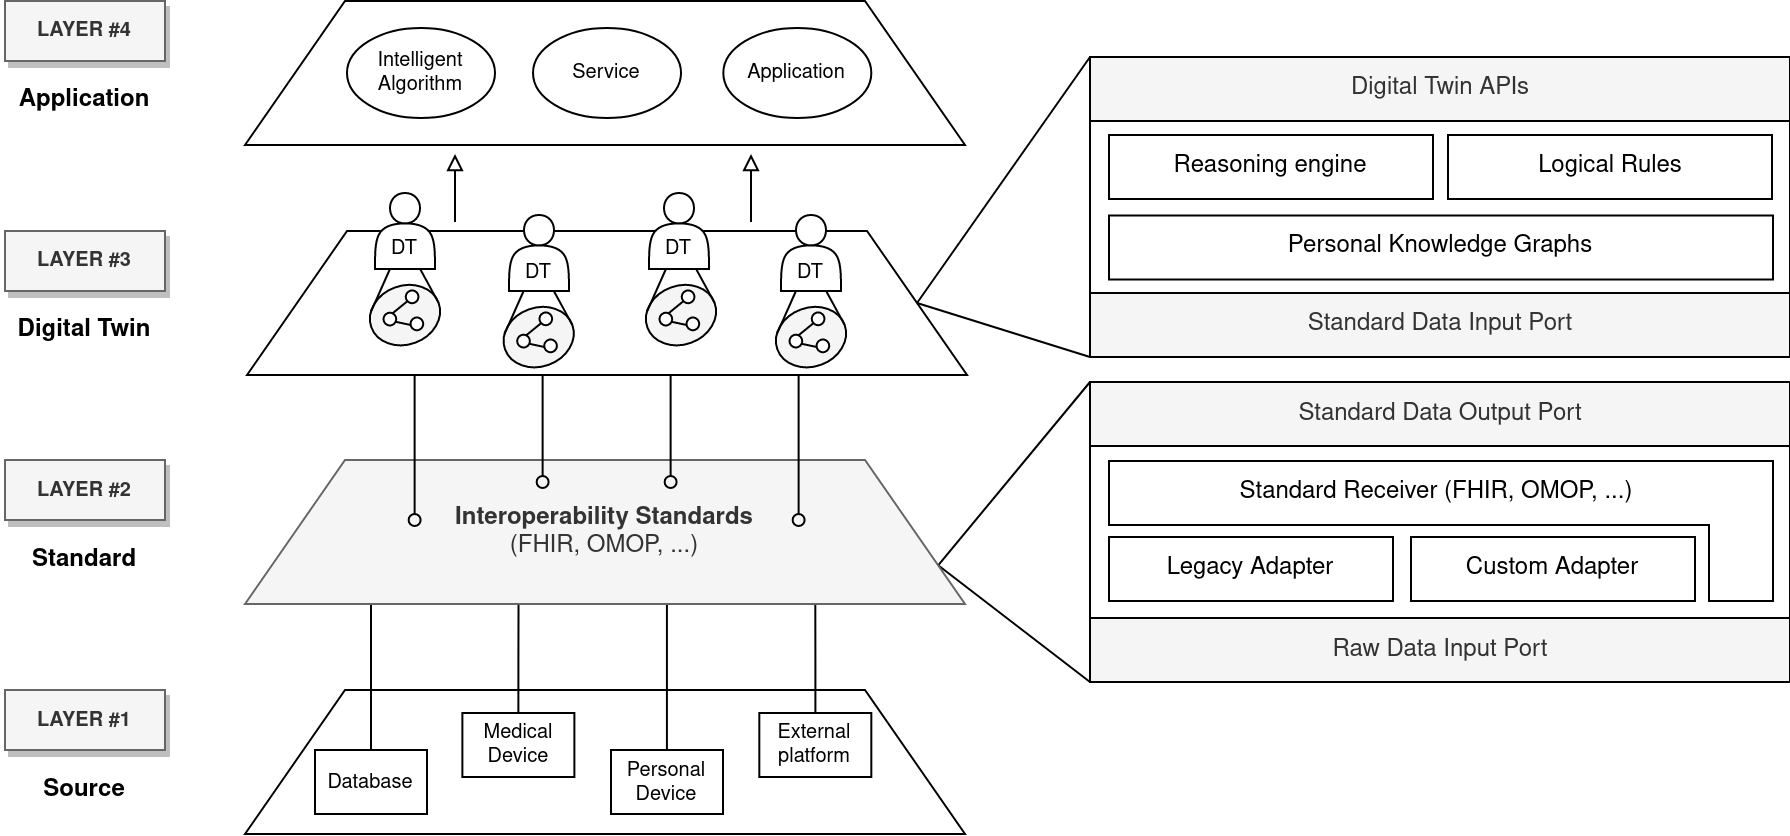
\includegraphics[width=\textwidth]{figures/paper4/Connected.png}
\end{center}
\caption{Illustration depicting the 4-tier architecture's former setup: data from the Physical Assets, modeled using FHIR resources, feed the state of the DTs for the overlying applications and services.}
\label{paper4_fig1}
\end{figure}

CONNECTED is designed in a microservices architectural style which consists of dividing services into a set of small services. Microservices architecture is considered well-suited for the modular development of flexible, evolving, and distributed systems such as the proposed architecture. Indeed, the microservices architecture offers elasticity. This is manifested in the ability to update the DT framework frequently during runtime. This practice reduces the software delivery time and provides the necessary flexibility to respond quickly and effectively to workload changes that edge and cloud resources may experience. Moreover, it enables seamless orchestration among multiple edge and cloud resources.

Considering the wide range of applications, the flexibility in interaction modes, and the evolution of the system, we consider the development of CONNECTED's microservices using the clean architecture pattern \cite{martin2017clean} that allows the separation of business logic from implementation specifications. In this case, the functionalities of the DT are made available externally through the use of adapters that can make use of specific libraries. Any modifications to the adapters will not affect the core logic of the DT.

The correct communication between the various services is an essential element for the functioning of the whole system. Among the most popular solutions for event-driven information exchange, the use of a message queue is particularly effective. In this asynchronous interaction approach, microservices do not dialogue directly with each other as they produce and consume messages by exploiting a central communication bus, favoring scalability, resilience in the event of disruptions of one or more system components, the decoupling of microservices and the flexibility in introducing new microservices into the system without having to make changes to other components. We adopted Apache Kafka, a distributed event streaming platform, the de facto standard for the implementation of message queues in the context of microservices architectures.

In the following section, we propose an enhancement of the existing CONNECTED architecture, integrating ML models with a formal, machine-readable description of their characteristics. This serves as a standard documentation of the models, possibly empowering the framework with additional capabilities, such as seamless integration of new models, and their coordination with existing algorithms or data sources.

\subsection{Representation of Machine Learning models within CONNECTED}\label{sec:paper4_representation}

Representing the DT as a mere repository of real-time data, while sufficient for certain use cases, does not fully utilize the capabilities of this paradigm. To achieve that, it is necessary to enhance our DT by enabling simulations. Therefore, we are actively striving to integrate ML models into our framework.

A recent survey has shown that up to 87\% of well-performing ML projects never get deployed due to integration issues\cite{venturebeat_why_2019}. A solution to this problem is the adoption of an MLOps workflow that promotes a smoother development experience throughout the whole ML lifecycle time. It results in the deployment of plenty of models through web services. These models can be described utilizing reports, i.e. documents that inform researchers, software developers, stakeholders, and interested persons (such as patients) about the specific model adopted, the inputs, the output, what the ML approach performs, and potential technical or ethical problems. A similar approach, using model cards, is suggested by NIH through their Bridge2AI programme to provide informative and transparent descriptions of ML models to stakeholders \cite{Amith2022}. Nonetheless, as a static document, they do limit opportunities to permit the information contained within the report to be computable.
We propose to pair every model with a Manifest: a machine-readable formal description that enriches the model with a detailed explanation of its interface, adopting existing standards and ontologies, such as LOINC, SNOMED-CT, and UOM. It essentially allows us to produce a computable version of the model that can be shared, reused, and linked. The adoption of the Manifest allows for the development of algorithms to automatically index models, aggregate their capabilities, and exploit them to deal with complex tasks. By using an ontology to construct our formal representation of ML models, we standardize the nomenclature and representation of ML model reports, essentially producing a computable version of the model that can be shared, reused, and linked. Manifests are computable artifacts, able to link information about ML models, leverage semantic reasoning to link the information, and open up software tooling opportunities, aggregation of models, and querying of the information for healthcare ML research.

After defining a bespoke ontology aimed at defining model manifests, we enhance CONNECTED by introducing a bridge linking the DT level (Layer 3) with the ML models. Its purpose is to empower the architecture with the ability to execute models. To do so, it parses Manifests and looks for the required ontological concepts within the patient KG, which will be automatically supplied as input to the respective model. 

Consider the integration of a hypothetical clinical ML model within our evolved framework, aimed at predicting an individual's risk of developing cardiovascular disease over the following decade. This model draws insights from a range of health indicators including blood pressure, cholesterol levels, and BMI. Stakeholders operating at Layer 4 can harness the diverse capabilities of this model, tailoring them to align with the distinctive profiles of patients through the use of the DT API. Specifically, the expanded Layer 3 accesses the model Manifest (Figure~\ref{paper4_fig2}), providing comprehensive descriptions of each health parameter using LOINC codes from the CONNECTED ontology. These codes facilitate the retrieval of precise values from the patient KG, essential as inputs for the model's computations (Figure~\ref{paper4_fig3}). Once the model completes its execution, the outcomes are conveyed back to the user in a standardized format via the DT API.

\begin{figure}
\begin{center}
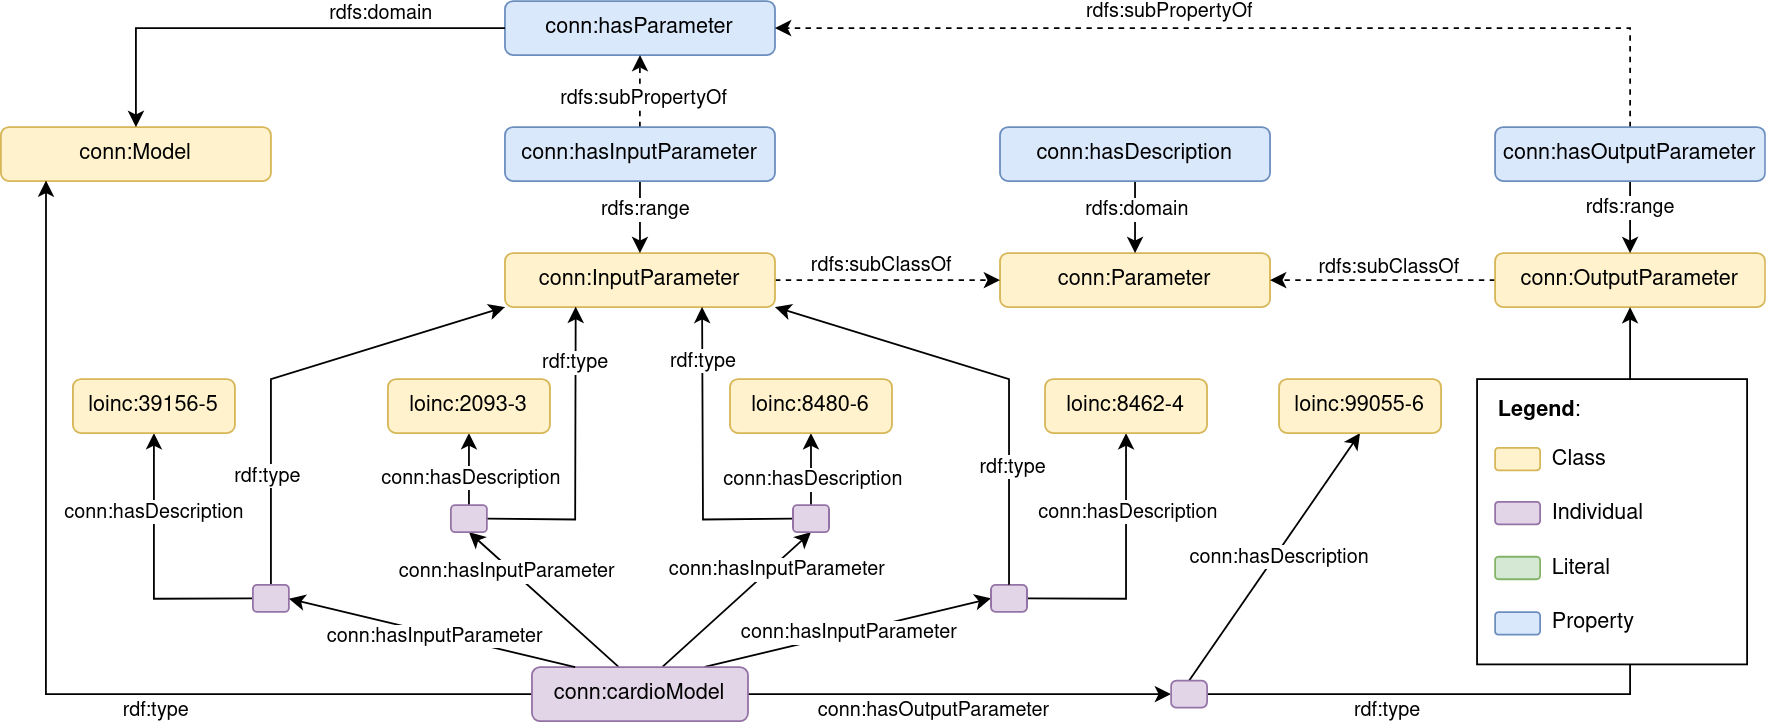
\includegraphics[width=\textwidth]{figures/paper4/connected-ontology-and-model.png}
\end{center}
\caption{RDF Representation of the cardiovascular disease prediction Manifest using the CONNECTED ontology (conn:). It integrates the LOINC ontology terms to uniquely identify the description of the inputs and output of the model.}\label{paper4_fig2}

\end{figure}

\begin{figure}
\begin{center}
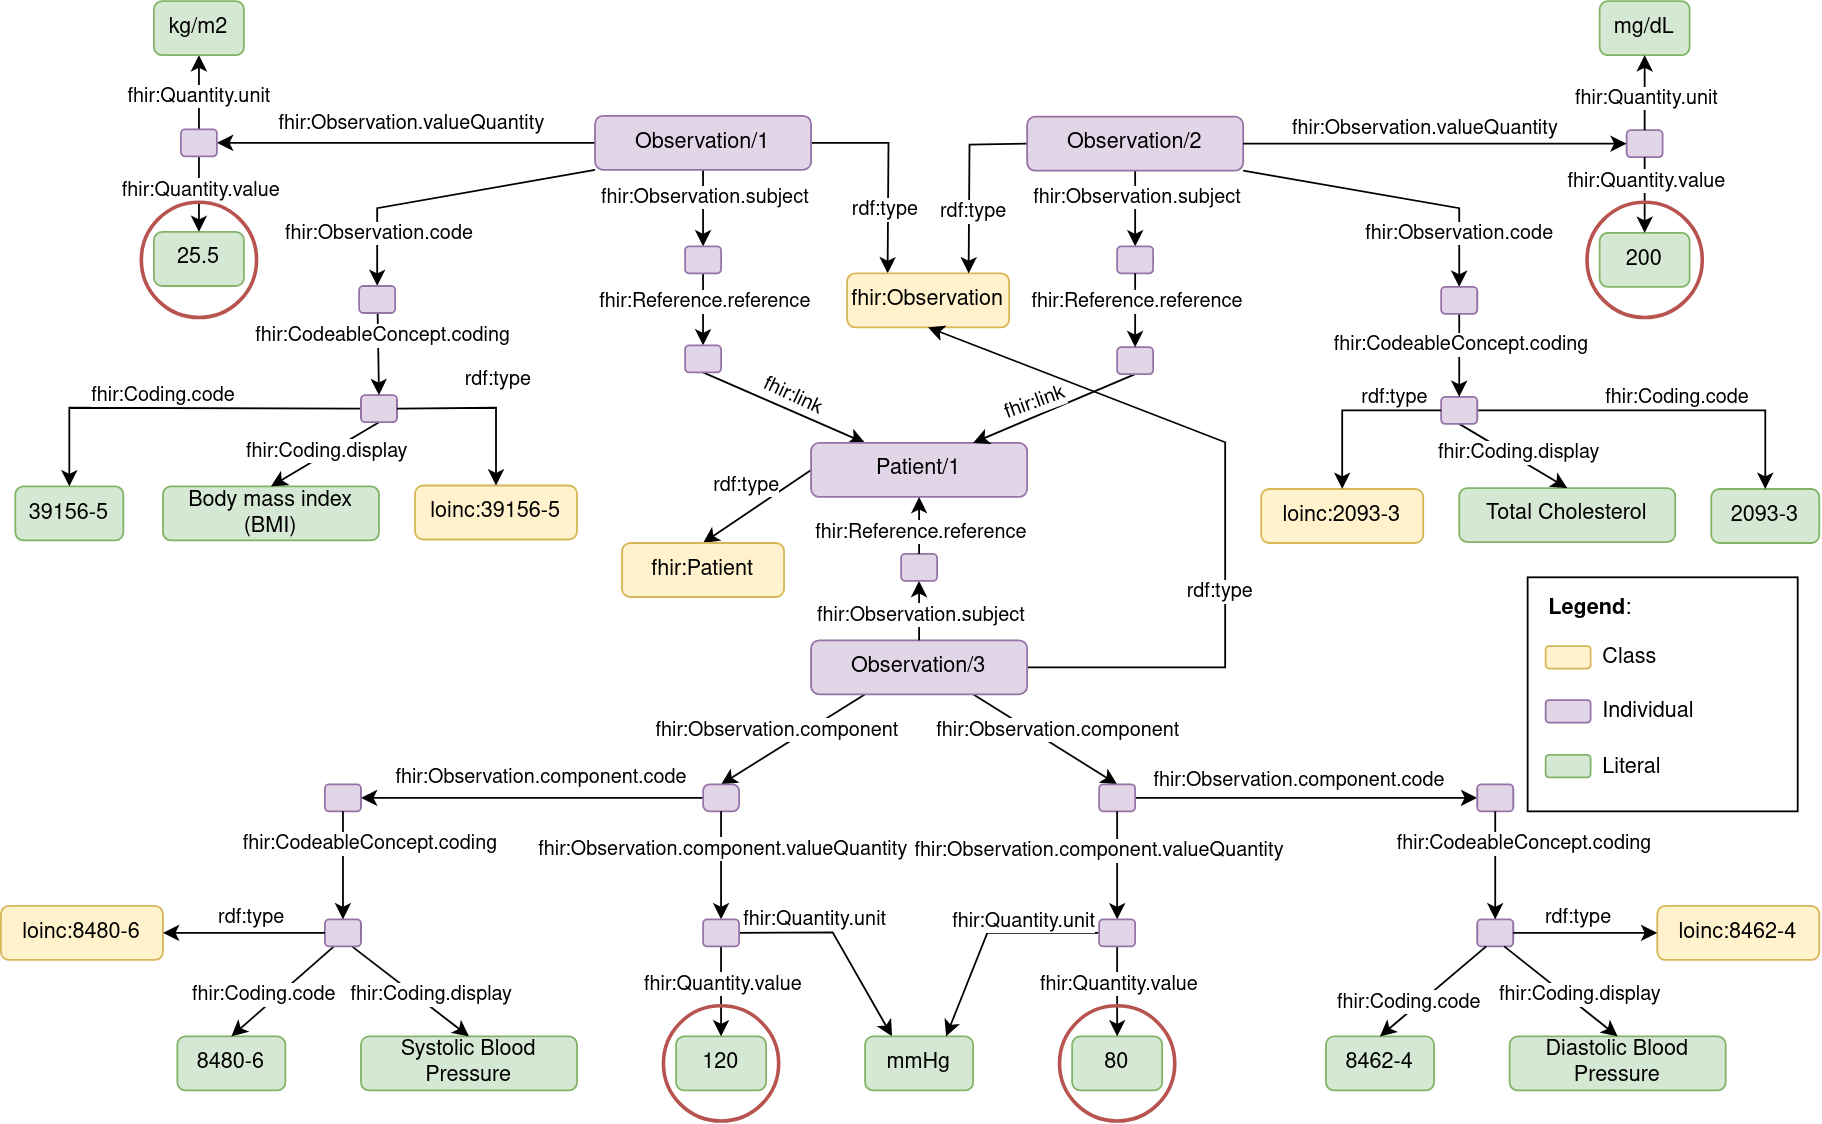
\includegraphics[width=\textwidth]{figures/paper4/patient-fhir-kg.png}
\end{center}
\caption{RDF Representation of a subset of the patient knowledge graph, that uses FHIR/RDF to describe clinical concepts. The marked nodes, being identified by a LOINC code, are those that will be fed to the cardiovascular risk prediction model.}\label{paper4_fig3}
\end{figure}

\subsection{Discussion and Conclusion}\label{sec:paper4_discussion}
This paper proposed the evolution of the CONNECTED conceptual framework, a multi-layered system designed to seamlessly integrate and standardize heterogeneous data sources, facilitating the realization of DTs supported by KGs. Our contribution lies in the introduction of the Manifest concept, which serves as a formal and machine-readable description for ML models, thereby enabling semantic reasoning. This key feature empowers the effective aggregation of these models and facilitates information retrieval regarding their usage. The proposed enhancement not only refines our current vision of DT but also introduces simulation capabilities and an ecosystem where models can be systematically indexed and leveraged. By having a clear description of the models, existing data can be fed automatically to them, improving their overall usability. Some benefits of this approach are: 
\begin{itemize}
    \item Model capabilities described by a document that is independent of a specific language, technology, or framework. 
    \item Detailed and standard description of a model feature, including input/output, through ontologies, dictionaries, etc. 
    \item Automatic/semi-automatic wiring of model input/output with patient data. 
    \item Personalizing generic ML models to specific patient features fosters tailored medicine approach. 
    \item Optionally, create a pipeline of models in which the output of one computation can become the input of the subsequent one. This pipeline could be first validated by matching the types and later executed on specific patients. 
    \item Enabling comparison of different models. 
\end{itemize}
We are applying the proposed extension to some use cases to verify how OWL2-based manifest can represent and formalize ML model information and to show the coverage and usefulness of our proposal in transforming static ML models into a computable format for machine-based processing.

\subsection*{Acknowledgment}
This study was partially supported by the Italian Ministry
of University and Research under PNRR-PNC Project
PNC0000002 ”DARE – Digital Lifelong Prevention” (CUP: B53C22006240001).

% layout: keep this paper's floats within its section
\FloatBarrier



\chapter{Inference and Reasoning}
\label{chap:inference_reasoning}

This chapter contains the two contributions associated with the \emph{Inference and Reasoning} stage described in Section~\ref{sec:inference_reasoning}: Paper~5 (Section~\ref{sec:paper5}) and Paper~6 (Section~\ref{sec:paper6}).

% ============================================================================
% Paper 5 -- integrated from papers/Frontiers___CONNECTED__Leveraging_Digital_Twins_and_Personal_Knowledge_Graphs_
% in_Healthcare_Digitalization/frontiers.tex (front matter transcribed from \Authors, \Address, \corrAuthor,
% \corrEmail, abstract and keywords; body converted mechanically, see the integration report).
% frontiers_SupplementaryMaterial.tex and test.bib in the same folder are unmodified Frontiers template files and
% contain no paper content; they are not integrated.
% ============================================================================
\section{CONNECTED: Leveraging Digital Twins and Personal Knowledge Graphs in Healthcare Digitalization}
\label{sec:paper5}

\noindent This section contains the article~\cite{10.3389/fdgth.2023.1322428_carbonaro_connected}.

\paragraph{Authors.}
Antonella Carbonaro\,$^{1,*}$, Alberto Marfoglia\,$^{1}$, Filippo Nardini\,$^{2}$ and Sabato Mellone\,$^{3}$

{\raggedright
\noindent\textsuperscript{1}Department of Computer Science and Engineering, Universit\`a di Bologna, Cesena, Italy\\
\textsuperscript{2}Department of Industrial Engineering, Universit\`a di Bologna, Bologna, Italy\\
\textsuperscript{3}Department of Electrical, Electronic, and Information Engineering ``Guglielmo Marconi'', Universit\`a di Bologna, Cesena, Italy\\
\textsuperscript{*}Corresponding author. E-mail address: antonella.carbonaro@unibo.it.\\
Front. Digit. Health 5 (2023) 1322428. doi: \url{https://doi.org/10.3389/fdgth.2023.1322428}. Received 16 October 2023; Accepted 27 November 2023; Published 7 December 2023.\\
\textcopyright{} 2023 Carbonaro, Marfoglia, Nardini and Mellone. This is an open-access article distributed under the terms of the Creative Commons Attribution License (CC BY).
\par}

\subsection*{Abstract}

Healthcare has always been a strategic domain in which innovative technologies can be applied to increase the effectiveness of services and patient care quality. Recent advancements have been made in the adoption of Digital Twins (DTs) and Personal Knowledge Graphs (PKGs) in this field. Despite this, their introduction has been hindered by the complex nature of the context itself which leads to many challenges both technical and organizational. In this article, we reviewed the literature about these technologies and their integrations, identifying the most critical requirements for clinical platforms. These latter have been used to design CONNECTED (COmpreheNsive and staNdardized hEalth-Care plaTforms to collEct and harmonize clinical Data), a conceptual framework aimed at defining guidelines to overcome the crucial issues related to the development of healthcare applications. It is structured in a multi-layer shape, in which heterogeneous data sources are first integrated, then standardized, and finally used to realize general-purpose DTs of patients backed by PKGs and accessible through dedicated APIs. These DTs will be the foundation on which smart applications can be built.

\paragraph{Keywords:} healthcare, digital twins, architectural framework, personal knowledge graphs, data integration

\subsection{Introduction}

In the era of rapid technological advancements, digitalization has become a game-changer in healthcare, with the potential to improve patient care quality and safety~\cite{engstrom_impact_2023}. However, the successful realization of the digital revolution requires addressing several issues such as data fragmentation, lack of interoperability, and management of vast streams of real-time data~\cite{mumtaz_current_2023}. Modern technologies, such as Digital Twin (DT), emerged as a response to these challenges~\cite{sun_digital_2023}, but they are usually designed to have a vertical perspective which limits their capability to synergistically cooperate~\cite{9325551_ricci}.  

On the other hand, precision medicine has been a hot topic in recent years, improving the effectiveness and decreasing the side effects of clinical treatments~\cite{cailleaux_fused_2021}. Personal Knowledge Graph (PKG) emerged as a promising solution to provide tailored services to its users~\cite{skjaeveland_ecosystem_2023}, offering a comprehensive and patient-centric perspective on the individual’s health. Hence, there is an urgent need for architectural guidelines aimed at facilitating the development of an ecosystem of Digital Twins capable of communicating, which will act as a foundation for the implementation of healthcare applications. 

In this perspective, we propose CONNECTED (COmpreheNsive and staNdardized hEalth-Care plaTforms to collEct and harmonize clinical Data), a conceptual multi-level framework aimed at integrating heterogeneous data sources using modern healthcare standards. The gathered information is fed to PKGs, which will support general-purpose patient DTs. Finally, custom applications can communicate with DTs through their APIs, realizing specific tasks, services, simulations, etc.

In the forthcoming sections, we will first review the existing literature on PKGs and DTs. Next, we will analyze current architectural approaches that incorporate these technologies, aiming to identify shared features. These highlighted characteristics will serve as the foundation for establishing the essential requirements that will guide the development of our framework.

\subsection{Recent Advancements in Personal Knowledge Graph}
In the existing literature, PKGs have been defined in multiple ways~\cite{skjaeveland_ecosystem_2023}. According to Balog and Kenter~\cite{balog_personal_2019}, a PKG is characterized as a source of structured knowledge about entities and their relationships, where the entities and relationships are of personal importance to the user. Diverging from conventional knowledge graphs, a PKG is intentionally crafted to capture an individual’s personal knowledge and experiences, embodying a spiderweb-like layout. Thus, the primary aim is to facilitate the provision of services tailored specifically to its owner. In the current landscape, there has been significant interest in the application of PKGs, which have been employed in several healthcare applications. 

Gyrard et al. propose a PKG framework aimed at developing personalized healthcare applications to effectively manage chronic disease~\cite{gyrard_personalized_2018}.
Rastogi and Zaki suggest that PKGs could be used to personalize recommendations from good platforms to encourage a healthy lifestyle~\cite{rastogi_personal_2020}.  
Ammar et al. present a mobile health digital intervention that combines both patients’ personal health data and contextual knowledge from various sources~\cite{ammar_using_2021}. The objective is to offer tailored recommendations for enhancing self-care behaviors among diabetic adults. Seneviratne et al. introduce a PKG that supports the generation of tailored dietary recommendations for Type 2 Diabetes self-management~\cite{seneviratne_personal_2021}. To do so, reasonings are made over the PKG, that encodes clinical guidelines represented in OWL. 

\subsection{Digital Twin in Healthcare}
DTs have found application in many healthcare sectors, such as oncology~\cite{sager_digital_2023}, cardiology~\cite{corral-acero_digital_2020}, geriatrics~\cite{liu_novel_2019}, neurology~\cite{voigt_digital_2021}, internal medicine~\cite{subramanian_digital_2020}, trauma management~\cite{croatti_integration_2020}, pharmaceutics~\cite{Björnsson2019}, orthopedics~\cite{aubert_development_2021}, surgery~\cite{heartflow_case_nodate}. 

Croatti et al. discussed the application of agent-based DTs to digitalize the process of severe trauma management, realizing a continuous monitoring~\cite{croatti_integration_2020}. A pre-hospital DT collects real-time information from the central unit, GPS systems, and smart rescuers’ equipment, registers the severity of the ongoing trauma decided by the rescuers, and automatically compiles emergency forms. Information is later sent to another DT aimed at managing the trauma process inside the hospital. Its life cycle evolves according to the macrosteps related to trauma and terminates when the patient is ready for hospitalization.

Björnsson et al. proposed to build DTs of patients, which can be computationally treated with thousands of drugs to find the optimal one, evaluating each one’s pros and cons~\cite{Björnsson2019}.  

Aubert et al. developed a virtual replica to evaluate stabilization method variants for tibial plateau fracture surgery at distinct stages of bone healing~\cite{aubert_development_2021}. It demonstrates how DTs can provide quantitative and high-value information for clinical decision-making. 

\subsection{Architectural Frameworks for Digital Twins}\label{sec:paper5_architectural-frameworks}
In the domain of DTs, the establishment of robust architectural frameworks serves as a cornerstone for molding their functionalities and expanding their utility~\cite{minerva_digital_2021}. This section delves into a selection of significant contributions that introduce architectural models designed to build and elevate DTs across different domains. After an analysis of each one, they will be summarized to highlight their main capabilities. Subsequently, these functionalities will provide the basis for developing our framework's requirements. 

Malakuti et al. provide an abstract four-layer architecture pattern to construct DTs in the industrial context~\cite{malakuti_four-layer_2019}. In their vision, the bottom layer consists of many heterogeneous information sources that feed data to the DTs through the Model layer, which aggregates information. The processed data is made accessible to applications through specialized DT APIs. Remarkably, this framework is intentionally engineered to be both extensible, accommodating a dynamic range of information sources, and flexible, enabling it to adeptly handle a variety of data types, making it a versatile foundation for DT development. 

Sahlab et al. conceptualize a multi-layer KG-based architecture for the application of DTs in Cyber-Physical Systems, providing improved capabilities, such as internal linking and referencing, knowledge completion, error detection, collective reasoning, and semantic querying~\cite{sahlab_knowledge_2021}. The result is the Intelligent DT, an evolution of the DT, equipped with a module for model comprehension using artificial intelligence to continuously adapt and learn. They propose a modular solution in which the communication between physical and virtual assets is bidirectional. It also includes a reasoning engine, aimed at deducing knowledge from heterogeneous models and running predictions of future states of the system. 

Ricci et al. discuss a vision in which healthcare, a complex domain, can be modeled as an open ecosystem of DTs, owned by different organizations, but designed to communicate and cooperate in the same scenarios~\cite{9325551_ricci}. In this perspective, DTs are not bound to a specific application, but they are thought more of as services exposing their APIs, leading to a Digital Twin-as-a-service approach. They shift away from the traditional vertical representation of DT, embracing a layered architecture in which their capabilities can be horizontally composed. Within this vision, DTs serves as a stable foundation on top of which applications and smart algorithms can be built. 

The work presented underlines features that address shared crucial needs of DT frameworks, from which it was possible to explicitly derive the requirements of CONNECTED: 

\begin{itemize}
    \item \textit{Real-time data streaming}: The framework must incorporate ports to enable the real-time flow of data streams. Therefore, it necessitates a layer capable of gathering real-time data from IoT devices, medical devices, smartphones, organizations, etc. 
    \item \textit{Heterogeneous sources integration}: It must be possible to collect data from diverse sources and feed them to the relevant DTs. To do that, the gathered information must be harmonized to a common domain model. Especially in the healthcare context, standards might facilitate this process, also improving interoperability across organizations.  
    \item \textit{Symbolic reasoning}: As Knowledge Graphs can effectively describe and manage healthcare information, by employing reasoning algorithms, they facilitate the derivation of insights regarding a patient's status and prognostications. Furthermore, the stored knowledge can be accessed through intuitive semantic queries, in an explorative search fashion. 
    \item \textit{General-purpose Digital Twin}: DTs should act as a foundation on top of which smart applications can be developed. Hence, they do not need to be aware of specific program details. In this regard, DTs can be represented by services exposing proper APIs, enabling effective communication with external software. 
\end{itemize}

\subsection{CONNECTED: a framework for general-purpose Digital Twins}
In this section we introduce CONNECTED, a conceptual framework aimed at defining guidelines to develop healthcare applications based on DTs of patients. It has been based on the requirements defined in the previous section, and it has been designed following a modular approach. Hence, the result is a multi-layer architecture in which functionalities are partitioned into horizontal levels (Figure \ref{fig:paper5_framework1}): \textit{Source}, \textit{Standard}, \textit{Digital Twin}, and \textit{Application}. The communication between them is monodirectional, so data can flow from one layer to the above one only by passing through designated input and output interfaces.  
 
\begin{figure}%[h!]
\begin{center}
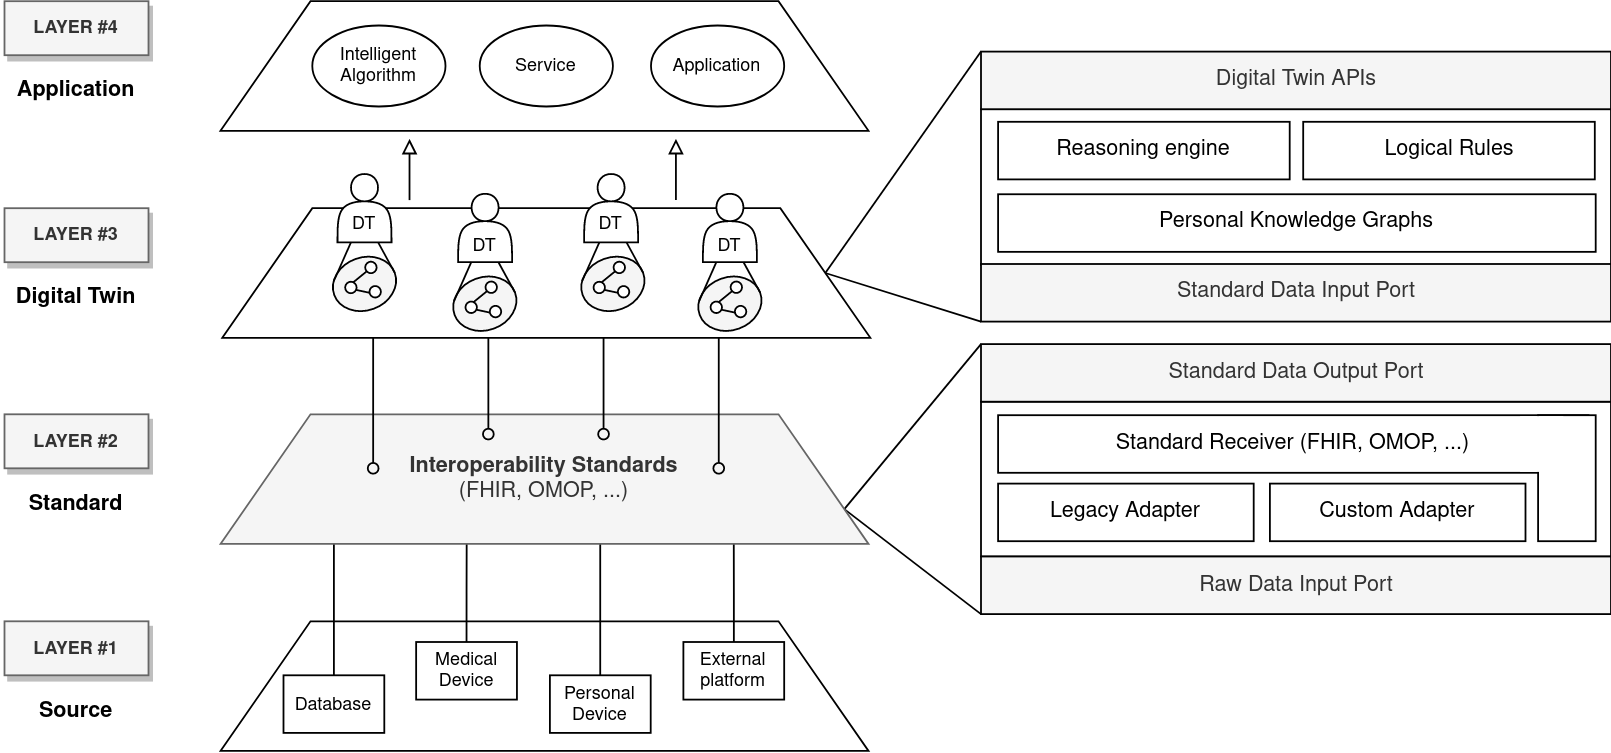
\includegraphics[width=1\linewidth]{figures/paper5/framework1.png}
\end{center}
\caption{Proposed four-layer architecture. Data flows from the lower levels to the upper ones.}\label{fig:paper5_framework1}
\end{figure}

\subsubsection{Level 1: Source}
In the healthcare context, a wide array of data sources exists, including personal and medical devices, as well as various platforms and databases. A key aspect of the proposed architecture is its capability to effectively communicate with these sources. 
Since incoming data may vary in terms of volume, quality, and format, the \textit{Source} layer functions as a sort of funnel. Its primary role is to efficiently manage this diverse information, accommodating different protocols for communication. Ultimately, its aim is to transmit the data stream to the higher-level layer. 

\subsubsection{Level 2: Standard}
The second level of the framework focuses on exploiting standards according to the interoperability requirement defined in Section \ref{sec:paper5_architectural-frameworks}. To this end, the adoption of a well-known solution, such as FHIR\footnote{https://www.hl7.org/fhir/}, proves essential in providing domain modeling that is validated by a vast international community of experts. This layer operates as a pipe, in which incoming raw data is harmonized and passed to the \textit{Digital Twin} layer. In this regard, this level must include submodules (\textit{Adapters} in Figure \ref{fig:paper5_framework1}) able to process data from legacy standards, and custom or proprietary formats to modern healthcare standards. 

\subsubsection{Level 3: Digital Twin}
To enhance our understanding of patients and their progress, we can utilize all the standardized data so far gathered to populate the DTs. From our perspective, these digital replicas serve as reliable sources of truth, enabling us to track a patient's evolution over time. While it doesn't provide simulation capabilities, this DT functions as a versatile repository of data that paints a comprehensive picture of the patient. This data can be leveraged to develop intelligent applications.

Given the heterogeneity of collected information and the constant evolution of the DT model, it is required a data structure capable of managing its changes and expressing semantic relationships between concepts. PKG is identified as an optimal solution to achieve that, as it allows us to capture personal information valuable for a specific subject and integrate it with general concepts of the healthcare domain. This can be done by taking advantage of web semantic tools such as ontologies (e.g., SNOMED-CT) and logical rules (e.g., SWRL). In fact, they can be provided as input to the semantic \textit{Reasoning Engine} aimed at automatically inferring new knowledge about the patient to support a well-informed decision-making process. 
Finally, DTs offer APIs to run explorative queries on single patients’ PKG. A matching subset of resources is returned to the caller.

\subsubsection{Level 4: Application}
Since Level 3 doesn't provide computational resources, the computational models implementing DT applications are located on Level 4. This layer hosts all the applications that need to observe the state of DTs, through their APIs. Following the previously defined requirements, an application is not bound to a single DT, whereas one DT may serve many. Examples of such clients include a wide range of applications, going from simple user interfaces to visualize patient information, to more sophisticated ones like smart assistants to support decision-making or monitoring systems.

\subsection{Validation}
In this section, we introduce a concrete scenario aimed at clarifying the framework data models and validating its expressiveness.
The chosen case study revolves around the identification and prediction of accidental falls in elderly patients, especially those suffering from osteoporosis, a critical domain that benefits from a comprehensive data analysis.
This entails capturing heterogeneous information, including patient activity preceding the accident, comprehensive EHR records (e.g medications, treatments, and previous CT scans), besides measuring the impact of the fall itself. 
In CONNECTED, these diverse data sources are managed in the \textit{Source} layer, and send messages towards the \textit{Standard} level.
Supposing \textit{Medical Device} is FHIR complaint, the fall data is already structured as an AdverseEvent FHIR resource, while data coming from EHR, being based on an HL7 legacy version, requires a conversion step, made by a default adapter (\textit{Legacy Adapter} in Figure~\ref{fig:paper5_framework2}), transforming it into FHIR resources. As concerns the step count tracked by the patient's \textit{Personal Device}, it operates using a proprietary format, requiring the development of an ad-hoc adapter (\textit{Custom Adapter} in Figure~\ref{fig:paper5_framework2}). The resulting information will be finally merged into the Patient DT existing PKG.
Leveraging this data will enable smart algorithms to estimate fracture risk for continuous monitoring, facilitating prompt emergency response, if necessary.

\begin{figure}
\begin{center}
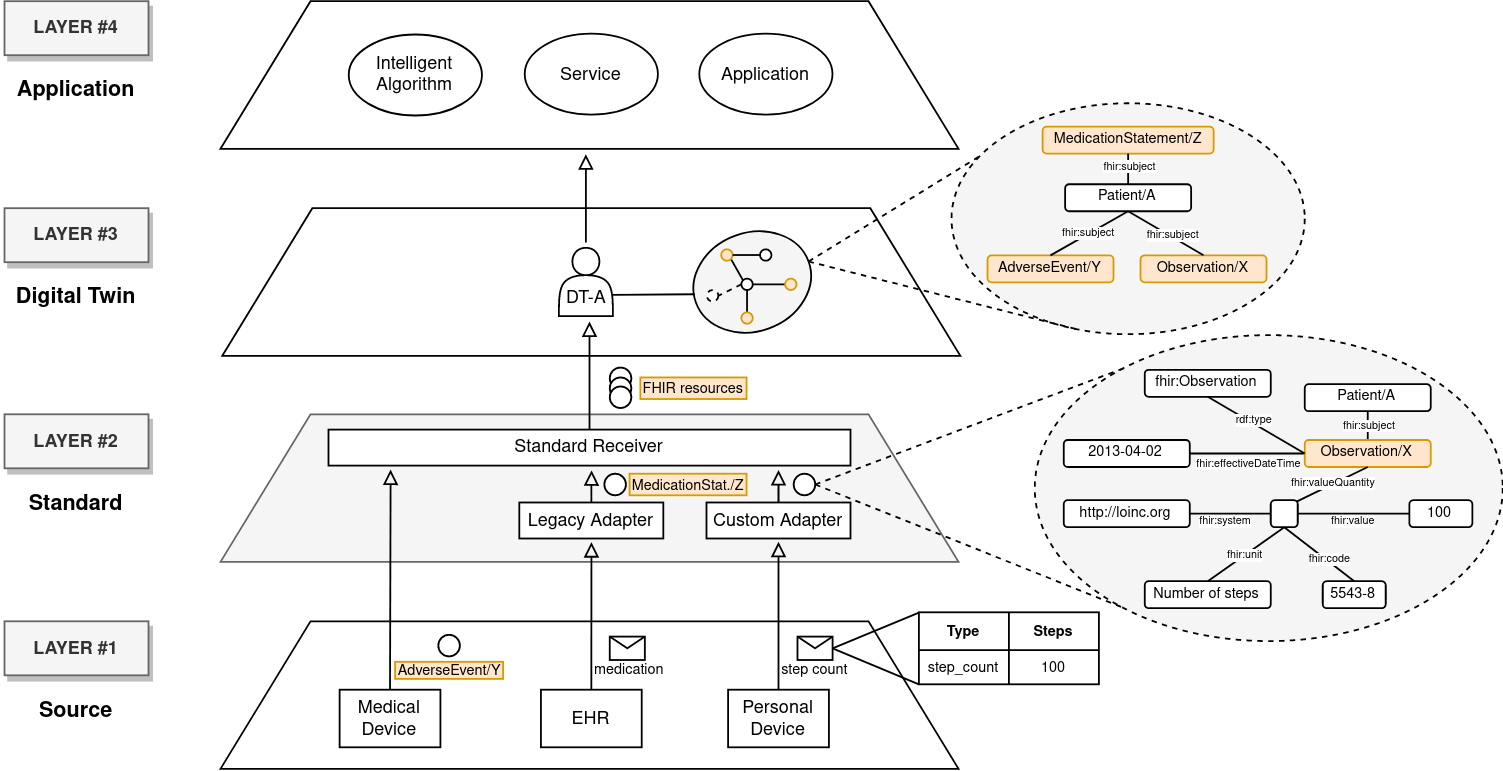
\includegraphics[width=1\linewidth]{figures/paper5/framework2.png}
\end{center}
\caption{Implementation of the proposed use case through the adoption of CONNECTED.}\label{fig:paper5_framework2}
\end{figure}

\subsection{Discussion}

In this article, we proposed CONNECTED, a modular framework in which various data sources are integrated through the adoption of modern healthcare standards, to feed general-purpose DTs of patients. Indeed, we identified PKGs as a solid backbone for DTs, given their ability to model heterogeneous data while keeping their high semantic expressiveness and to enable semantic search, supported by a reasoner, which is ideal for complex, dynamic, and rapidly changing environments such as healthcare. General-purpose DTs act as a source of truth and establish a foundation to design and develop smart applications. At last, we presented a use case aimed at validating CONNECTED expressiveness.

Within this perspective, several challenges are yet to be addressed, given the high sensitivity of healthcare data. From a technical point of view, it is fundamental to guarantee the integrity and validity of collected data, ensuring the reliability of the information stored in the PKGs, and fostering their backbone role within the framework. Another primary concern is related to PKG realization. For example, if many PKGs are extracted by a unique underlying graph, it is hard to trace a clear boundary between distinct patients. On the other hand, if PKGs are physically separated, information might be duplicated, possibly leading to inconsistencies. To this end, access-control policies must be implemented to allow specific stakeholders to query only the DTs for which they are given rights.  
Furthermore, due to the nature of treated information, it is worth mentioning that this kind of platform must deal with complex legal, ethical, and regulatory issues, such as different privacy policies of distinct organizations. 

Future work will focus on selecting the best-suited technologies for implementing the proposed framework and its adoption in real-use case healthcare scenarios. In this regard, we are currently developing a solution aimed at unveiling the issues and practical challenges associated with the concrete implementation of the framework. Specifically, we are evaluating the use of Eclipse Hono~\footnote{https://projects.eclipse.org/projects/iot.hono} for the \textit{Source} layer. This technology empowers the architecture with the ability to communicate with a multitude of IoT devices, regardless of the communication protocol, as well as supporting custom adapters for data transformation. 
Afterward, standardized data streams are channeled through a distributed and asynchronous message bus, implemented using Apache Kafka~\footnote{https://kafka.apache.org/}. These streams ultimately converge on DTs, where they are stored in a graph database. Our choice for this database is Stardog~\footnote{https://www.stardog.com/}, primarily due to its capacity to enable information querying and knowledge inference through the utilization of a reasoner.
Our aim is to release the resulting prototype as open-source software for readers to validate them. Finally, further extensions of the framework should be investigated, such as the possibility of integrating computational models into the existing vision of DT, enabling simulation capabilities.

\subsection*{Conflict of Interest Statement}
The authors declare that the research was conducted in the absence of any commercial or financial relationships that could be construed as a potential conflict of interest.

\subsection*{Funding}
This study was partially supported by the Italian Ministry of University and Research under PNRR-PNC Project PNC0000002 ”DARE – Digital Lifelong Prevention” (CUP: B53C22006240001).

% layout: keep this paper's floats within its section
\FloatBarrier


% ============================================================================
% Paper 6 -- integrated from papers/_FGCS____DIGITA_25_extended__camera_ready_(1)/cas-dc-template.tex (front
% matter transcribed from the cas-dc \title/\tnotetext/\author/\affiliation, abstract, highlights and keywords;
% body converted mechanically, see the integration report). The source contains \credit{} commands but
% \printcredits is commented out, so no CRediT statement is printed (as in the source).
% ============================================================================
\section{A Knowledge Graph-Driven Framework for Deploying AI-Powered Patient Digital Twins}
\label{sec:paper6}

\noindent This section contains the article~\cite{MARFOGLIA2026108380}.

\paragraph{Authors.}
Alberto Marfoglia\textsuperscript{1,*}, Christian D'Errico\textsuperscript{1}, Sabato Mellone\textsuperscript{2}, Antonella Carbonaro\textsuperscript{1}

{\raggedright % layout: ragged-right metadata block
\noindent\textsuperscript{1}Dept. of Computer Science and Engineering - DISI, University of Bologna, Cesena, Italy\\
\textsuperscript{2}Dept. of Electrical, Electronic and Information - DEI, Engineering ``Guglielmo Marconi'', Bologna, Italy\\
\textsuperscript{*}Corresponding author: Alberto Marfoglia (alberto.marfoglia2@unibo.it)\\
E-mail addresses: alberto.marfoglia2@unibo.it (A. Marfoglia), christian.derrico2@unibo.it (C. D'Errico), sabato.mellone@unibo.it (S. Mellone), antonella.carbonaro@unibo.it (A. Carbonaro).\\
ORCID: \url{https://orcid.org/0009-0000-5857-2376} (A. Marfoglia), \url{https://orcid.org/0009-0002-5784-0492} (C. D'Errico), \url{https://orcid.org/0000-0001-7688-0188} (S. Mellone), \url{https://orcid.org/0000-0002-3890-4852} (A. Carbonaro). \\
Future Generation Computer Systems 180 (2026) 108380. \url{https://doi.org/10.1016/j.future.2026.108380}. Received 20 May 2025; Received in revised form 23 October 2025; Accepted 16 January 2026; Available online 20 January 2026.\\ 0167-739X/\textcopyright{} 2026 The Author(s). Published by Elsevier B.V. This is an open access article under the CC BY license (\url{http://creativecommons.org/licenses/by/4.0/}). 
\par}

\subsection*{Abstract}

Background: The healthcare sector faces diverse challenges, including poor interoperability and a lack of personalized approaches, which limit patient outcomes. Ineffective data exchange and one-size-fits-all treatments fail to meet individual needs. Emerging technologies like digital twins (DTs), the semantic web, and AI show promise in tackling these obstacles. For this reason, we introduced CONNECTED, a conceptual multi-level framework that combines these techniques to deploy general-purpose patient DTs.
%
Objective: This study assesses CONNECTED's comprehensiveness, applicability, and utility for developing intelligent, personalized healthcare applications. Specifically, we deliver a preliminary version of the framework to predict future patient states and demonstrate its automation benefits in deploying semantically enriched, AI-powered patient DTs.
%
Methods: We enhanced the CONNECTED architecture by providing a formal definition of DT and modularizing its core functionalities into microservices—Properties, State, Capabilities, and Manifest. The Manifest service facilitates AI model integration through the Model Interface Manifest Ontology (MIMO), enabling automatic data-to-model binding via a reasoner. Using the HeartBeatKG quality assessment tool, we validated MIMO and tested the internal logic by integrating a well-established stroke-risk model.
%
Results: Our implementation comprehends: (1) deploying a FHIR-compliant, patient-centric API for clinical history access, real-time monitoring, and predictive simulation; (2) publishing MIMO; (3) establishing the Manifest protocol for seamless, general-purpose AI model integration tailored to individual patient profiles; and (4) a proof-of-concept benchmarking application comparing multiple stroke risk classifiers.
%
Conclusion: CONNECTED establishes a flexible, scalable foundation for interoperable semantic patient DTs. Automation reduces technical overhead and enables users to focus on delivering personalized, insight-driven care.

\subsection*{Highlights}

\begin{itemize}
\item Enable patient digital twin deployment via a knowledge-driven, modular framework
\item Provide clinical data access and simulation through a FHIR-compliant API
\item Publish MIMO ontology to standardize and increase transparency of AI model interfaces
\item Automate AI model integration using a manifest-based binding protocol
\item Benchmark stroke risk models with real-time, time-aware clinical data streams
\end{itemize}

\paragraph{Keywords:} Digital Twins; Healthcare; Knowledge Graphs; Machine Learning Models; Pervasive Computing; Semantic Web; Personalized Medicine; Predictive Analytics

\subsection{Introduction}~\label{paper6_introduction}
The ongoing digital transformation of healthcare is reshaping how care is delivered, driven by the increasing need to integrate heterogeneous, real-time data streams and provide more personalized, patient-centered services \cite{engstrom_impact_2023,amri_data-driven_2023}. These advancements promise improved precision in diagnosis and treatment, reduced side effects, and greater patient empowerment \cite{engstrom_impact_2023,cailleaux_fused_2021}.
%%%% CHANGED: 
%However, realizing this potential remains challenging due to fragmented data sources, a lack of interoperability, and the absence of scalable architectures that support seamless communication across systems \cite{mumtaz_current_2023}.
%%%% TO:
However, the full realization of these advancements remains constrained by fragmented data ecosystems, limited interoperability, and the absence of scalable, knowledge-driven architectures capable of unifying data and services across institutions~\cite{mumtaz_current_2023}.

Digital Twins (DTs), virtual replicas that continuously mirror the status and behavior of physical systems, are gaining traction in healthcare as tools for real-time patient monitoring \cite{johnson_digital_2024}, personalized treatment planning \cite{vallee_digital_2023}, and optimizing clinical operations \cite{sun_digital_2023}. Yet, despite their promise, current healthcare DTs face several limitations. These include the difficulty of multi-scale modeling, limited access to high-quality and standardized clinical data for validation \cite{arcobelli2024fhir,marfoglia_towards_2025}, and rigid, vertically designed architectures that inhibit interoperability and reuse across settings \cite{9325551_ricci}.
%%%% CHANGED:
%%%% TO:
Therefore, enabling interoperable, semantically enriched, and AI-augmented DT frameworks is essential to realize the vision of continuous, personalized, and predictive healthcare.

Concurrently, Artificial Intelligence (AI) and the Internet of Things (IoT) are automating time-intensive clinical tasks, particularly in domains such as precision imaging \cite{johnson_precision_2021}. While AI is expected to become central in advancing integrated, data-driven healthcare systems \cite{gupta_artificial_2021}, its effectiveness depends heavily on high-quality, multi-modal data and rigorous real-world validation. In addition, using AI in clinical decision-making raises ethical challenges related to transparency, explainability, and accountability \cite{sun_ai_2023}.

Knowledge representation is another cornerstone of intelligent healthcare systems. Among the most effective tools in this area are knowledge graphs (KGs), which structure complex, interconnected data to improve integration, reasoning, and scalability \cite{peng_knowledge_2023}. In healthcare, KGs help bridge data silos and enhance decision support by facilitating semantic interoperability and trust in machine-generated insights \cite{peng_knowledge_2023,abu-salih_healthcare_2023}.

To address these architectural and integration challenges while unifying the strengths of DTs, AI, and KGs, we propose CONNECTED (COmpreheNsive and staNdardized hEalth-Care plaTforms to collEct and harmonize clinical Data) \cite{10.3389/fdgth.2023.1322428_carbonaro_connected}, a multi-level framework for deploying general-purpose patient DTs following a DTs-as-a-service (DTaaS) approach. CONNECTED is designed to aggregate clinical data across sources, support real-time monitoring, and ensure interoperability through semantic web technologies. In its original conception, CONNECTED enabled patient DTs to store structured clinical histories as KGs and provide dynamic status updates on demand \cite{10.3389/fdgth.2023.1322428_carbonaro_connected}.

We then extended CONNECTED by equipping DTs with predictive simulation capabilities powered by AI models \cite{marfoglia_2024_mimo}. To enable their seamless integration, we designed the Manifest protocol. Each model is accompanied by an RDF machine-readable formal description, called  Manifest, which specifies the functional requirements needed to execute it, such as input, output, location, and runtime constraints. Once uploaded into the framework, each Manifest can be linked to patient-specific DTs via the Capability abstraction defined in CONNECTED's DT Layer.

The Manifest protocol enables automatic integration of AI models, regardless of algorithmic implementation, communication protocol, or hosting environment. The Capability abstraction further enhances model potential by tailoring general-purpose models to the unique characteristics of each patient, thus supporting personalized care. Moreover, because both model interfaces and DT states are represented semantically as KGs, CONNECTED can automatically extract the required patient data, invoke the model with appropriate inputs, and record the outputs as predictive outcomes within the DT. This degree of automation and the CONNECTED API significantly reduces the technical burden on users, allowing them to focus on insight-driven decision-making.

This paper evaluates CONNECTED's comprehensiveness, applicability, and utility for developing intelligent and personalized healthcare applications. We introduce a preliminary implementation designed to forecast patient health trajectories and demonstrate its ability to automate the deployment of semantically enriched, AI-powered DTs. 

Our implementation achieves four key contributions:
\begin{itemize}
    \item A FHIR-compliant, patient-centric API that enables access to clinical histories, real-time monitoring, and predictive simulation;
    \item The publication of the Model Interface Manifest Ontology (MIMO) in the Linked Open Data Cloud (LOD) to support transparent and standards-based model descriptions;
    \item The implementation of the Manifest protocol, enabling automated data-to-model binding and seamless integration of general-purpose AI models into patient DTs;
    \item A proof-of-concept benchmarking application built on the CONNECTED API, enabling the dynamic integration, evaluation, and comparison of multiple stroke risk classifiers. Incoming data streams drive continuous, time-aware model selection and performance ranking.
\end{itemize}
%%%% CHANGED:
% The remainder of this paper is structured as follows. Section~\ref{sec:related_work} surveys related work on healthcare DTs and foundational frameworks, positioning our contributions within the current landscape. Section~\ref{sec:architectural_background} describes the CONNECTED architecture and its core components. Section~\ref{sec:results} presents the core results, including the FHIR-compliant DT API, the MIMO ontology, the implementation of the Manifest protocol for stroke risk classification, and a proof-of-concept benchmarking application. Finally, Section~\ref{sec:discussion} discusses limitations and outlines future research directions.
%%%% TO:
The remainder of this paper is structured as follows. Section~\ref{sec:paper6_related_work} surveys related work on healthcare DTs and foundational frameworks, positioning our contributions within the current landscape. Section~\ref{sec:paper6_architectural_background} presents the CONNECTED architecture, followed by the implementation details in Section~\ref{sec:paper6_implementation}. Section~\ref{sec:paper6_manifest_protocol} describes the Manifest protocol, and Section~\ref{sec:paper6_evaluation} presents our evaluation results. Section~\ref{sec:paper6_discussion} provides a broader discussion of findings and limitations, outlining future research directions.

\subsection{Related Work}~\label{sec:paper6_related_work}
DT frameworks have seen growing interest across multiple domains. However, most existing solutions originate from industrial applications~\cite{wang_mobility_2022}and are not well-suited to the unique challenges of healthcare. These include heterogeneous clinical data integration, adherence to stringent interoperability standards, and the need for patient-centered design. As a result, many general-purpose DT architectures lack the semantic, dynamic, and modular features required for medical applications.
%
%%%% CHANGED:
%\subsection{Healthcare-Specific DT Efforts}
%%%% TO:
\subsubsection{Patient-Centric DT Initiatives}
Several efforts have sought to tailor DTs to clinical use cases. Saxby et al.~\cite{saxby_digital_2023} explored DTs for neuromusculoskeletal modeling, demonstrating their utility for tendon strain analysis and neurorehabilitation. However, their approach lacks standardized mechanisms for data exchange, limiting scalability and integration potential.

In a more patient-specific approach, Rad et al.~\cite{sarani_rad_personalized_2024} present a DT framework for diabetes management using Personal Knowledge Graphs (PKGs). Although their use of FHIR-aligned ontologies supports data integration and real-time decision-making, they do not offer a patient DT formal definition or provide reusable implementation artifacts, limiting reproducibility.

Similarly, Jameil et al.~\cite{jameil_digital_2025} integrate IoT and hybrid machine learning for anomaly detection in real-time monitoring. Despite technical maturity, their work conflates DT and AI components and does not propose a modular, generalizable framework for semantic model integration.
%
%%%% CHANGED:
%\subsection{Semantic and Knowledge-Driven Architectures}
%%%% TO:
\subsubsection{Knowledge-Driven Architectures}
KGs are increasingly leveraged to enhance semantic interoperability and reasoning in DTs. Jinzhi et al.~\cite{jinzhi_exploring_2022} propose a KG-based DT framework with reasoning capabilities to forecast future states. However, it lacks healthcare-specific adaptability and contextualization.

Sahlab et al.~\cite{sahlab_knowledge_2021} introduce a KG-enhanced DT framework for Cyber-Physical Systems (CPS), supporting internal linking, error detection, and semantic querying. While rich in knowledge processing, the framework struggles with integrating digital artifacts and lacks standard data formats, making AI model integration cumbersome.

Lee et al.~\cite{lee_digital_2025} explore the construction of PKGs using SNOMED CT and LOINC to support AI-driven healthcare services. Their design emphasizes longitudinal patient records but lacks temporal reasoning capabilities and a clear DT formalization, hindering real-time adaptability and personalization.
%
\subsubsection{Foundational Frameworks}
At a more abstract level, Angelelli et al.~\cite{pellegrino_conceptual_2025} offer a conceptual framework that identifies 11 key dimensions for DT evaluation in healthcare, including modularity and interoperability. While useful as a design compass, it lacks empirical validation and does not provide implementation strategies or code artifacts.

Ricci et al.~\cite{9325551_ricci} propose a service-oriented architecture using horizontally layered, API-driven components to improve composability and interoperability. While conceptually aligned with modern software principles, their framework remains under-specified in implementation. Specifically, they omit mechanisms for semantic integration, AI model binding, or patient-level personalization—features central to real-world deployment.

Lombardo et al.~\cite{LOMBARDO2024107203} address real-time learning through a DT architecture focused on intelligent location-based services. Although capable of continual adaptation, the system lacks patient-centered care mechanisms and does not leverage semantic representations, limiting its relevance for personalized clinical applications.

\subsubsection{Summary and Differentiation}
Across prior work, a recurring gap emerges between conceptual richness and implementation maturity. Many frameworks offer theoretical contributions or single-purpose prototypes, but fall short in three critical areas:
%
\begin{enumerate}
    \item A formal definition of patient-specific DTs: specifying their responsibilities and functional boundaries. For example, what types of patient data can be retrieved and observed? What kinds of simulations can be performed? DTs remain abstract and difficult to standardize or operationalize without such a definition.
    \item Semantic-level interoperability: the ability to automatically interpret and integrate data across heterogeneous systems using shared ontologies and standard vocabularies. A key challenge is to collect, harmonize, and store vast amounts of clinical data while preserving, and ideally enriching, its semantic meaning.
    \item Modular integration of AI models: enabling algorithms to be seamlessly connected to patient data in a plug-and-play fashion, supporting personalized and predictive care with minimal manual configuration. A robust framework should provide an abstraction layer between AI models and DT functionalities to support continuous integration, model comparison, and replacement. This facilitates dynamic evaluation and selection of the most appropriate model for predicting specific patient trajectories.
\end{enumerate}
%
CONNECTED addresses these challenges by offering both a conceptual and technical solution. Conceptually, it organizes functionalities into a layered architecture and defines a patient-oriented DT model. Technically, it delivers:
%
\begin{itemize}
    \item A microservice-based architecture that exposes DT functionalities through a FHIR-compliant RESTful API, enabling access to clinical histories, observation of current patient states, and execution of predictive simulations;
    \item The Manifest protocol and MIMO to describe, bind, and execute AI models in a transparent, reusable, and interoperable manner;
    \item The use of semantic web technologies to harmonize and enrich patient data and AI model interfaces. This allows automatic data-to-model matching and ensures consistent knowledge management as the ecosystem evolves.
\end{itemize}
%
Through this combination, CONNECTED offers a generalizable and scalable foundation for intelligent, patient-centered DTs in healthcare, reducing technical overhead while overcoming long-standing barriers to standardization, semantic interoperability, and modular AI integration.

%%%% CHANGED:
% \section{Methods}~\label{sec:methods}
%%%% TO:
\subsection{Architectural background}~\label{sec:paper6_architectural_background}
%%%% CHANGED:
%This section presents the architectural and methodological foundations underpinning the CONNECTED framework.
%It aims to address key challenges in real-time data integration, semantic interoperability, and intelligent service orchestration by abstracting the complexity of physical systems and offering a uniform digital representation of patients. Inspired by the cyber–physical abstraction principles and the DTaaS paradigm, CONNECTED structures its components to support scalable, interoperable, and domain-agnostic applications.

% The following subsections outline the design principles, system architecture, and semantic technologies that constitute the core of the CONNECTED platform.
%%%% TO:
This section provides a concise recap of the CONNECTED architecture and the DT conceptual model. For a comprehensive extended discussion of the original design principles and motivation, the reader is referred to our prior works~\cite{10.3389/fdgth.2023.1322428_carbonaro_connected,marfoglia_connected_2025}.

%%%% CHANGED:
% \subsection{From Data Sources to Services: A Multi-Layered Approach}
%%%% TO:
\subsubsection{Multi-layer Architecture}
This CONNECTED framework introduces a multi-layer architecture (Figure~\ref{paper6_fig1}) comprising four key layers: \textit{Source}, \textit{Standard}, \textit{Digital Twin}, and \textit{Application}, each responsible for a specific function within the system. The framework employs a modular, layered structure to manage data flows and decouple services, providing flexibility and robustness in handling heterogeneous data sources and dynamic healthcare requirements. Each framework's layer plays a critical role in ensuring the smooth flow of data and functionality between physical systems and high-level applications.
%
\begin{figure}
    \centering
    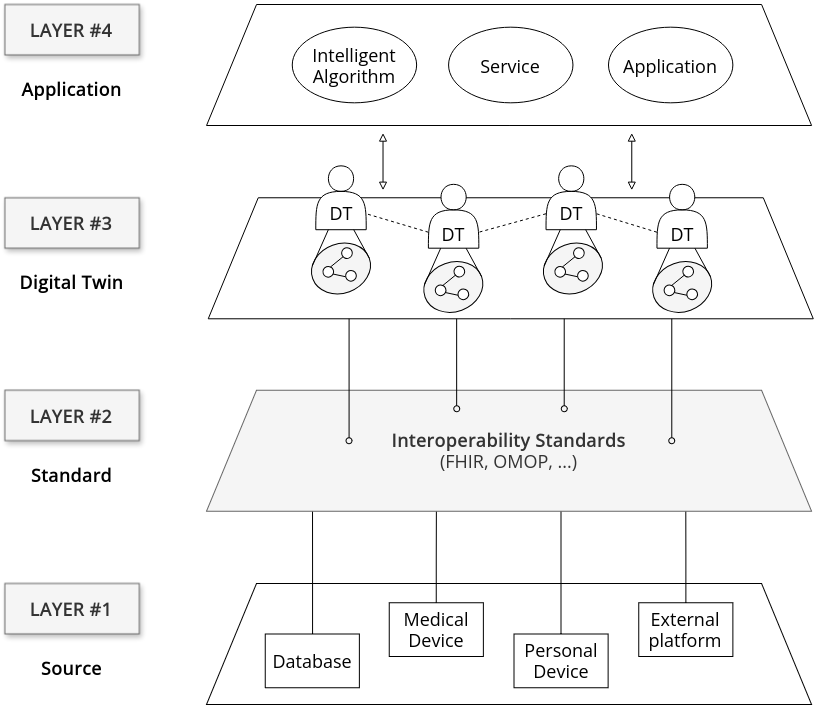
\includegraphics[width=1\linewidth]{figures/paper6/fig1.png}
    \caption{Diagram of the 4-tier architecture setup: data from the sources, structured with FHIR resources, are used to update the DTs' states, enabling functionality for applications and services in the highest layer.}\label{paper6_fig1}
\end{figure}
%
The Source Layer collects data in real-time from a wide array of devices, including medical and IoT devices, smartphones, and healthcare platforms. This layer functions as a data funnel, handling varying data volumes, formats, and protocols. It preprocesses the incoming data to ensure it is ready for further processing in the next layer.

The Standard Layer ensures interoperability across heterogeneous systems by adopting well-established healthcare standards such as FHIR. Incoming data is harmonized and transformed into a common format that supports interoperability across different devices and platforms. This layer includes adapters to process data from legacy and proprietary formats, facilitating integration with modern healthcare standards.

At the heart of the framework, the DT Layer creates virtual replicas of physical patients. These DTs enable real-time monitoring, retrieval of clinical history, and predictive analytics. This layer structures the collected data by employing KGs and ontologies to support advanced reasoning and inference, enabling the generation of insights into patient health.

The Application layer hosts applications that interact with the DTs via APIs. These applications range from simple visualization tools to complex decision-support systems that assist clinicians in decision-making. This layer leverages the data and capabilities provided by the DTs to deliver personalized and preventive care services. The API-driven architecture ensures that applications are not tightly coupled to specific DTs, enhancing the system’s flexibility and scalability.
%
%%%% CHANGED:
% \subsection{The Role of the Digital Twin Paradigm}
%%%% TO:
\subsubsection{Digital Twin Model}
The DT paradigm is an abstraction that bridges physical and digital layers of healthcare systems. DTs in CONNECTED are not static replicas, but intelligent, evolving entities that unify data from diverse sources, support semantic reasoning, and expose actionable interfaces for clinical applications. Healthcare data arises from heterogeneous sources (e.g., wearables, medical devices, and hospital systems) using different formats and protocols. The DT Layer abstracts this complexity by harmonizing inputs into a consistent digital representation. This cyber–physical decoupling enables the provision of a uniform abstraction and service level functionality to upper layers. In this way, these latter can focus on analysis and decision-making without needing to manage low-level infrastructural details. 

Each DT operates as an independent service under the DTaaS paradigm, exposing well-defined RESTful APIs to access state, trigger simulations, and retrieve derived insights. This modular design allows applications to interact with DTs in a scalable and reusable way, avoiding domain-specific silos.

Beyond mere data mirroring, each DT maintains a KG that semantically integrates heterogeneous, real-time data with domain ontologies and logical rules. This semantic layer supports reasoning over the patient's condition, enabling the inference of clinical states, risk factors, or behavioral trends, essential for preventive and personalized care.

In our framework, the DT serves as a virtual patient replica, describing the patient’s pathophysiology through three primary components:
\begin{itemize}
    \item \textbf{Properties}: A set of immutable attributes that define the identity and core characteristics of the patient, such as demographic data. By isolating fixed identifiers, Properties ensure consistency across systems, simplify data linkage, and reduce update complexity, supporting long-term traceability.
    \item \textbf{State}: A dynamic, time-sensitive information representing the patient’s evolving condition, including vital signs and clinical observations. The state supports real-time monitoring, which can be retrieved at any point as a historical snapshot. It also supports a shadowing mechanism to remain synchronized with incoming data, ensuring digital fidelity.
    \item \textbf{Capabilities}: A set of virtual operations or simulations the DT can perform, powered by algorithms that process its State and Properties to predict health outcomes or support clinical decisions. Moreover, Capabilities decouple prediction goals from implementation strategies, enabling the definition and comparison of multiple approaches to achieve the same objective.
\end{itemize}
%
\subsection{Platform implementation}\label{sec:paper6_implementation}
The implementation presented in this paper realizes the conceptual architecture summarized in Section~\ref{sec:paper6_architectural_background}. 
%%%% CHANGED:
%%%% TO:
Developing CONNECTED introduces several challenges, many of which fall outside the scope of our research. To address this, we have refined the platform's features based on the following assumptions: (i) The Application Layer can be emulated using a straightforward REST client, such as Postman; (ii) Data from the Source Layer are reliable, conform to the FHIR model, and include the DT's identifier; (iii) Any required data preprocessing is handled directly by the models, and (iv) Communication between the source and higher layers operates on a push-based model. 
%%%% CHANGED:
%These considerations enable us to concentrate on the DT Layer, as its development can contribute novel insights to the scientific community.
%Below we describe the concrete choices, microservice decomposition, and data-flow mechanisms that constitute the platform built for the experiments and validation reported in Section~\ref{sec:results}.
%%%% TO:
These assumptions allow us to focus primarily on the DT Layer, as its design and implementation can contribute novel insights to the scientific community. The following sections describe the concrete implementation choices, microservice decomposition, and data-flow mechanisms that form the basis of the platform used for the experiments and validation discussed in Section~\ref{sec:paper6_evaluation}.
%
%%%% CHANGED:
% \subsection{From Conceptual to a Microservice Implementation}
%%%% TO:
\subsubsection{Microservice Architecture}
The multi-layered structure of CONNECTED, combined with its diverse use cases and evolving requirements, led us to adopt a microservices architecture; a detailed description is provided in~\cite{marfoglia_connected_2025}. This approach improves maintainability by isolating components, minimizes interdependencies between services, and offers the flexibility needed to scale and adapt to future demands. By adhering to the information-hiding principle, each microservice exposes only minimal interfaces, thereby managing the system's complexity. Additionally, microservices avoid shared state or storage, enabling independent deployments and reducing the risk of system-wide failures.

A key challenge in a microservices architecture is defining clear service boundaries. From domain-driven design, services are segmented by business domains rather than specific functionalities. This domain-oriented approach simplifies feature development and integration, making it more cost-effective to introduce new capabilities or combine existing ones, rather than altering established services.

Each microservice follows the hexagonal architecture pattern~\cite{martin2017clean}, decoupling core business logic from external dependencies such as frameworks and libraries. This isolation ensures that DT functionalities remain agnostic to the implementation. By organizing internal modules in this layered, "onion-like" structure, we increase flexibility, streamline collaboration across teams, and simplify the development of unit tests.
%%%% CHANGED:
%%%% TO:
\subsubsection{Digital Twin Layer Services}
The functionalities of the DT Layer are structured into four independent Ktor web services (Figure \ref{paper6_fig2}): Model, Capability, State, and Property. The Manifest service allows the uploading, updating, and deleting of manifests, while the other three provide concrete implementations of the DT conceptualization introduced in the previous subsection. Additionally, we have developed a DT Manager that oversees the addition and modification of DT instances, ensuring the integrity of DT identifiers and maintaining consistency between the State and Capability services. Moreover, the Capabilities service interacts with a MongoDB database to store associations between DT and Manifest identifiers. Finally, we implemented an authentication service to manage user access to the platform and an NGINX gateway that exposes the CONNECTED API while concealing internal business logic.

\begin{figure}
    \centering
    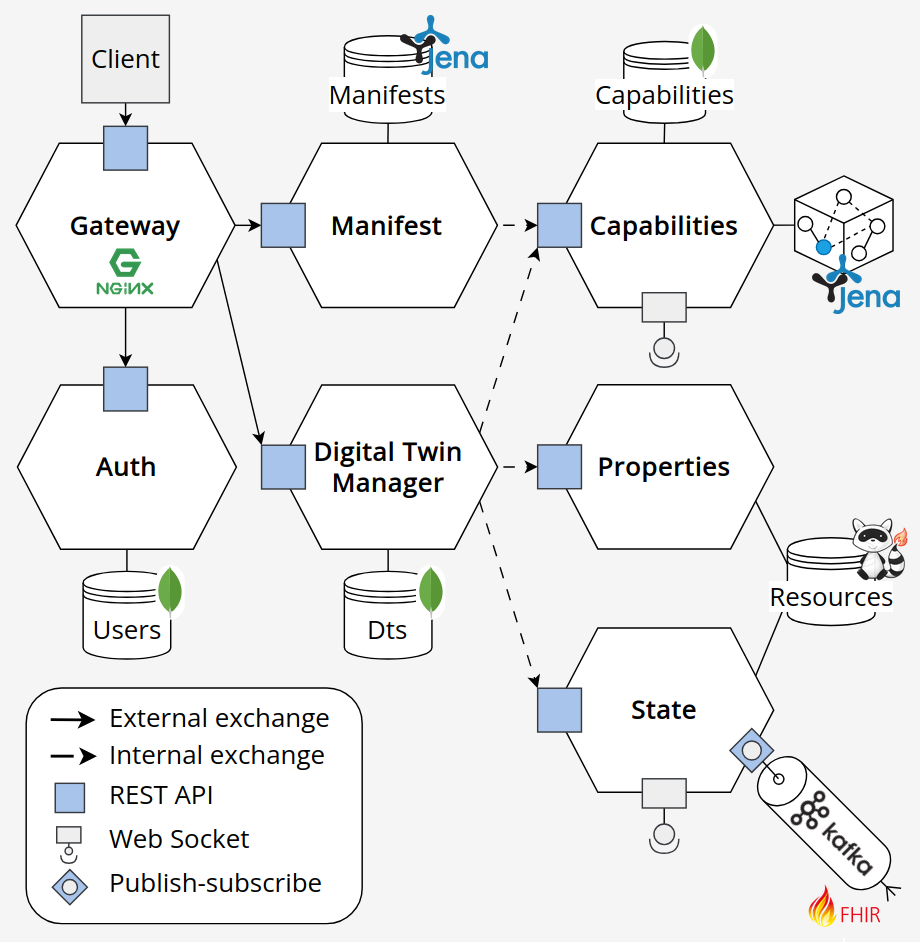
\includegraphics[width=1\linewidth]{figures/paper6/fig2.png}
    \caption{Micro-services architecture of the Digital Twin Layer.}\label{paper6_fig2}
\end{figure}

The domain modeling phase was notably time-intensive due to the heterogeneity of concepts across the various services. The Manifests uploaded are transformed into RDF graphs via the Jena RDF API and stored on a Fuseki server. We leveraged the FHIR specification to model the information describing the patient DT. Specifically, the FHIR Patient resource represents the Properties acting as the root linking all other standard resources (Observation, Encounter, etc.), modeling the State. The HAPI FHIR library facilitates development by providing a comprehensive Java implementation of the FHIR standard along with other utilities, including a client for effective interaction with FHIR-compliant services.

The system employs synchronous, blocking communication for both internal and external interactions, with a few key exceptions. In the Source Layer, data from external services and devices is converted into events and published to a Kafka event bus for asynchronous processing. Additionally, WebSockets enable real-time communication to exchange simulation results and monitor the state evolution of the DT.
%
%%%% CHANGED:
% \section{AI Model Semantic Binding via the Manifest Protocol}
%%%% TO:
\subsection{Manifest Protocol}\label{sec:paper6_manifest_protocol}
In CONNECTED, each DT can expose unique capabilities to predict future patient trajectories. These capabilities are underpinned by general-purpose AI models tailored to specific patient characteristics, which are activated upon triggering. Our framework seamlessly integrates the models through the Manifest protocol and automates all the crucial steps behind the execution of a DT capability: (1) takes a snapshot of the patient state and converts it into a KG; (2) retrieve the Manifest associated to that capability; (3) checks if the model interface can be fulfilled with the extracted data; (4) accesses and executes the models returning the result as soon as available.

%%%% CHANGED:
%%%% TO:
To evaluate the Manifest protocol, we selected a Neural Network classifier for stroke prediction originally proposed by Dev et al.~\cite{dev_predictive_2022}. We wrapped the model in Python, deployed it through a Flask web service, and independently recalculated its key performance metrics, including precision, recall, F1-Score, accuracy, miss rate, and false positive rate. Model validity was confirmed by ensuring that its accuracy fell within the distribution range reported by the authors. We then defined a Manifest instance describing the model's input requirements and registered it within CONNECTED. This enabled fully automated execution of the model via the Capabilities service. The metrics derived from Manifest-driven execution were compared with those from the baseline to confirm functional equivalence.

To further demonstrate the model-agnostic nature of the Manifest protocol, we also integrated a Decision Tree and Random Forest classifiers from Dev et al.'s study~\cite{dev_predictive_2022}. A dedicated Manifest instance was created for each model and uploaded within the infrastructure. These Manifests were then used to develop a proof-of-concept benchmarking application leveraging the framework’s RESTful APIs. This application showcases the semantic generality and technical flexibility of the Manifest protocol, which supports AI models regardless of their internal logic or complexity and validates the expressiveness of the CONNECTED API.

The Manifest protocol offers a level of automation that alleviates the technical burden on users, enabling them to concentrate on insight-driven decision-making. Its development required two distinct efforts: (a) the MIMO ontology to describe the AI models' interfaces, and (b) the implementation of the DT Capabilities component. 
%%%% CHANGED:
%%%% TO:
\subsubsection{MIMO: Design and Publication}
MIMO was designed following the Noy and McGuinness 1O1 Development Guide~\cite{mcguninnes}, and then implemented using the Protégé editor. It functions as a task ontology, capturing structural and operational aspects of executable models. It formally defines their interfaces as a combination of metadata, such as inputs, outputs, and location. We publicly released the MIMO ontology as a generalizable specification into the LOD repository to support reproducibility and promote reuse. Moreover, we documented MIMO using LODE (Live OWL Documentation Environment), a tool that automatically extracts ontology entities and generates human-readable HTML documentation based on their metadata \footnote{\url{https://model-interface-manifest-ontology-ad0613.gitlab.io/}}. Finally, the ontology was validated leveraging KGHeartBeat, an open-source KG quality assessment tool.
%%%% CHANGED:
%%%% TO:
\subsubsection{Semantic Binding and Orchestration}
The Capabilities component is realized as a dedicated microservice responsible for orchestrating model execution. When a specific capability is invoked, the service retrieves the required patient data and the corresponding model manifest by querying RESTful APIs exposed by the other services. These data sources are transformed into RDF-based KGs using the Jena RDF API and dynamically loaded into an in-memory graph at runtime.

A Jena reasoner, configured with OWL Description Logic (DL) rules and the Simulation and Integration Model Ontology (SIMO), is then applied to perform semantic inference. SIMO serves as a bridge between the model-centric MIMO schema and FHIR-compliant patient data representations. Notably, SIMO has not been published, as it is a task-specific application ontology developed to implement internal integration logics that are not intended for reuse beyond this context. The reasoner infers correspondences between a model’s input parameters and the patient data. Once valid mappings are established for all required inputs, the Capabilities service automatically triggers execution of the associated predictive model.

%%%% CHANGED:
%To evaluate the Manifest protocol, we selected a Neural Network classifier for stroke prediction originally proposed by Dev et al.~\cite{dev_predictive_2022}. We wrapped the model in Python, deployed it through a Flask web service, and independently recalculated its key performance metrics, including precision, recall, F1-score, accuracy, miss rate, and fall-out rate. Model validity was confirmed by ensuring that its accuracy fell within the distribution range reported by the authors. We then defined a Manifest instance describing the model's input requirements and registered it within CONNECTED. This enabled fully automated execution of the model via the Capabilities service. The metrics derived from Manifest-driven execution were compared with those from the baseline to confirm functional equivalence.
%
%To further demonstrate the model-agnostic nature of the Manifest protocol, we also integrated a Decision Tree and Random Forest classifiers from Dev et al.'s study~\cite{dev_predictive_2022}. A dedicated Manifest instance was created for each model and uploaded within the infrastructure. These Manifests were then used to develop a proof-of-concept benchmarking application leveraging the framework’s RESTful APIs. This application highlights the Manifest protocol's semantic generality and technical flexibility, which support AI models regardless of their internal logic or complexity, and validate the CONNECTED API's expressiveness.
%%%% TO:
%
\subsection{Evaluation and Experimental Results}~\label{sec:paper6_evaluation}
This section presents the principal outcomes of our work, structured around four core contributions: (1) the design and implementation of the DT Layer as a FHIR-compliant, patient-centric API enabling structured access to clinical history, real-time monitoring, and predictive simulation; (2) the development of the Model Interface Manifest Ontology (MIMO), published as LOD and evaluated through the HeartBeatKG quality assessment tool; (3) the validation of the Manifest protocol by integrating a well-established Neural Network model to identify patients at high risk of stroke; (4) the demonstration of the framework’s potential through a benchmarking proof-of-concept application that supports continuous evaluation of multiple stroke risk classifiers;
%%%% CHANGED: 
%%%% TO: 
and (5) a performance evaluation quantifying the platform’s scalability, latency, and throughput under concurrent workloads.
%%%% CHANGED:
% \subsection{Enabling Digital Twin Services through FHIR-Compliant API}
%%%% TO:
\subsubsection{FHIR-compliant API for DT Services}
Implementing CONNECTED opens new opportunities for healthcare applications by leveraging patient-specific DT to enhance clinical decision-making and streamline care delivery. 
%%%% CHANGED:
%%%% TO:
Unlike conventional systems that primarily provide raw data retrieval or event-based alerts, CONNECTED’s DTs offer a continuous, context-aware, and predictive representation of each patient. The platform’s FHIR-compliant REST API enables users to:
\begin{itemize}
    \item Retrieve comprehensive clinical histories, offering unified access to patient-centric, multi-source data.
    \item Monitor real-time health updates in the context of each patient’s evolving condition.
    \item Perform predictive simulations using integrated AI models, enabling clinicians to anticipate potential clinical trajectories.
\end{itemize}
%
This subsection illustrates these three core API-driven capabilities through UML sequence diagrams that reveal the system’s internal coordination. Each diagram focuses on the high-level orchestration among the framework's microservices, abstracting away lower-level infrastructure components such as authentication mechanisms, persistence layers, and proxy servers. The result is a clear and concise view of the logical information flow required to support each clinical use case.

\paragraph{Retrieving Patient Clinical History}
This operation allows external systems or applications to access a structured, comprehensive snapshot of a patient’s current and historical medical data. Specifically, the system returns a FHIR Bundle that encapsulates all relevant resources representing the patient's state at a given time. Figure~\ref{fig:paper6_clinical_history_sequence} illustrates that only the State service is required to fulfill the request.

% UML Sequence Diagram for Clinical History Retrieval
\begin{figure}
    \centering
    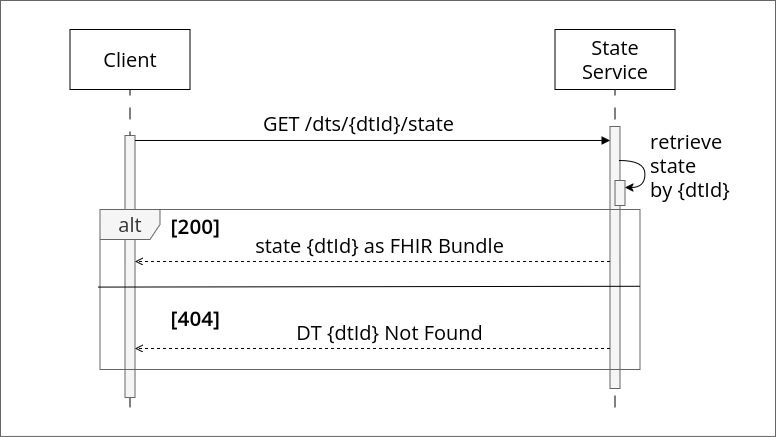
\includegraphics[width=1\linewidth]{figures/paper6/fig5.png}
    \caption{UML sequence diagram illustrating the patient’s clinical history retrieval request.}
    \label{fig:paper6_clinical_history_sequence}
\end{figure}

\paragraph{Real-time Monitoring of Patient Updates}
CONNECTED enables real-time patient monitoring by supporting continuous data streaming from each patient's DT to subscribed client applications. This capability is vital in dynamic clinical settings, where immediate access to the most current patient data is essential for timely and informed decision-making.

As depicted in Figure~\ref{fig:paper6_real_time_monitoring_sequence}, updates to the DT’s state are delivered via a persistent WebSocket connection and formatted in FHIR. Each state change is propagated as soon as it is registered within the system. For example, a medical device can trigger an update by publishing an event to the Kafka broker within the Source Layer. This event-driven architecture ensures low-latency data delivery and high responsiveness, facilitating seamless integration with real-time applications such as clinical dashboards, alerting mechanisms, and decision support systems.

\begin{figure}
    \centering
    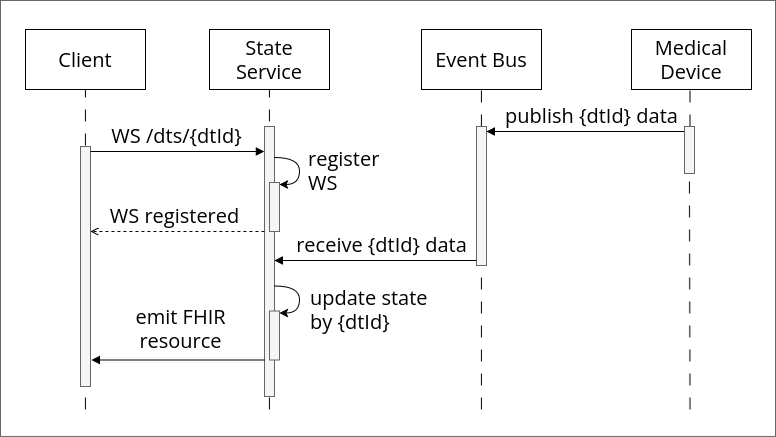
\includegraphics[width=1\linewidth]{figures/paper6/fig6.png}
    \caption{UML sequence diagram illustrating the patient real-time monitoring.}
    \label{fig:paper6_real_time_monitoring_sequence}
\end{figure}

\paragraph{Prediction of Patient Trajectories}
Among CONNECTED’s most advanced capabilities is its support for predictive simulations over patient-specific DTs by executing AI models defined via Manifests. This functionality empowers clinicians and healthcare applications to anticipate future clinical trajectories, such as the likelihood of disease onset or progression, based on a patient's most recent health status.

As shown in Figure~\ref{fig:paper6_predictive_trajectory_sequence}, a predictive request is initiated when the client application invokes a capability exposed by the patient’s DT. The platform then performs semantic alignment between the AI model’s input requirements specified in the Manifest and the current patient data encoded in the DT. If the necessary input parameters are available, CONNECTED automatically triggers the model execution through its dedicated API (labeled \texttt{Executable AI Model} in Figure~\ref{fig:paper6_predictive_trajectory_sequence}).

Given the potential computational cost of model inference, the framework executes prediction tasks asynchronously. Once the computation is completed, the prediction result is delivered back to the client via a WebSocket channel. This asynchronous design ensures non-blocking interactions, system scalability, and timely delivery of model outputs without compromising the user experience.

\begin{figure*}
    \centering
    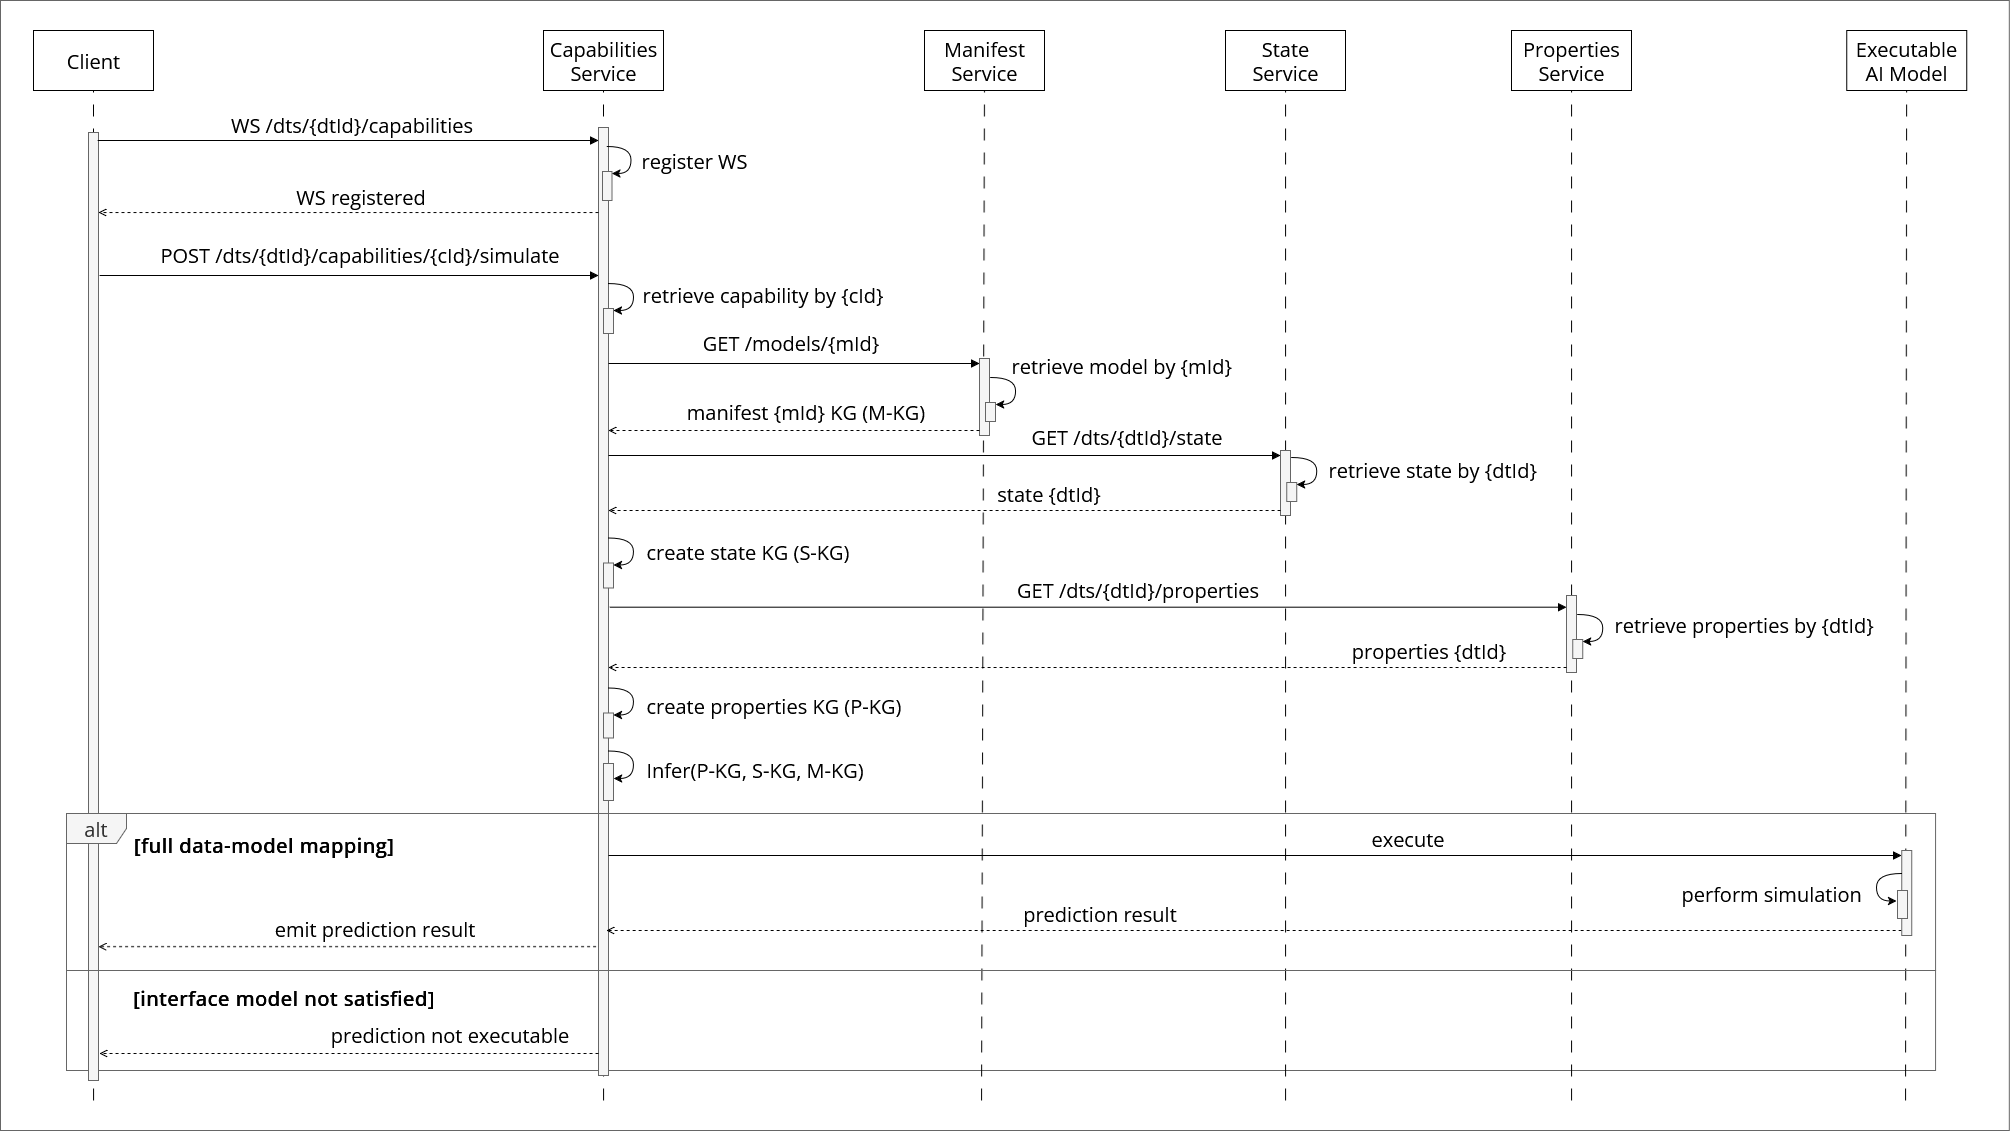
\includegraphics[width=1\linewidth]{figures/paper6/fig7.png}
    \caption{UML sequence diagram illustrating the prediction of future patient trajectories.}
    \label{fig:paper6_predictive_trajectory_sequence}
\end{figure*}

\subsubsection{MIMO: Ontology Quality Assessment}
MIMO was developed to formalize and support semantic descriptions of AI models for automated integration within DT architectures. The ontology was encoded in both OWL/XML (\texttt{.owl}) and Turtle (\texttt{.ttl}) serializations and is publicly available via our repository\footnote{\url{https://gitlab.com/unibo-connected/model-interface-manifest-ontology}}. It has also been published in the LOD\footnote{\url{https://lod-cloud.net/dataset/CONNECTED}}, ensuring discoverability, reuse, and interoperability across the semantic web ecosystem. The final release includes approximately 13 classes, 12 object properties, 8 data properties, and 65 logical axioms. The core foundational version contained 278 elements.

Figure~\ref{paper6_fig3} illustrates the core conceptual structure of MIMO, including its integration of Dublin Core annotation properties. These design choices enrich the ontology with standardized metadata and enhance semantic expressiveness.

\begin{figure}
    \centering
    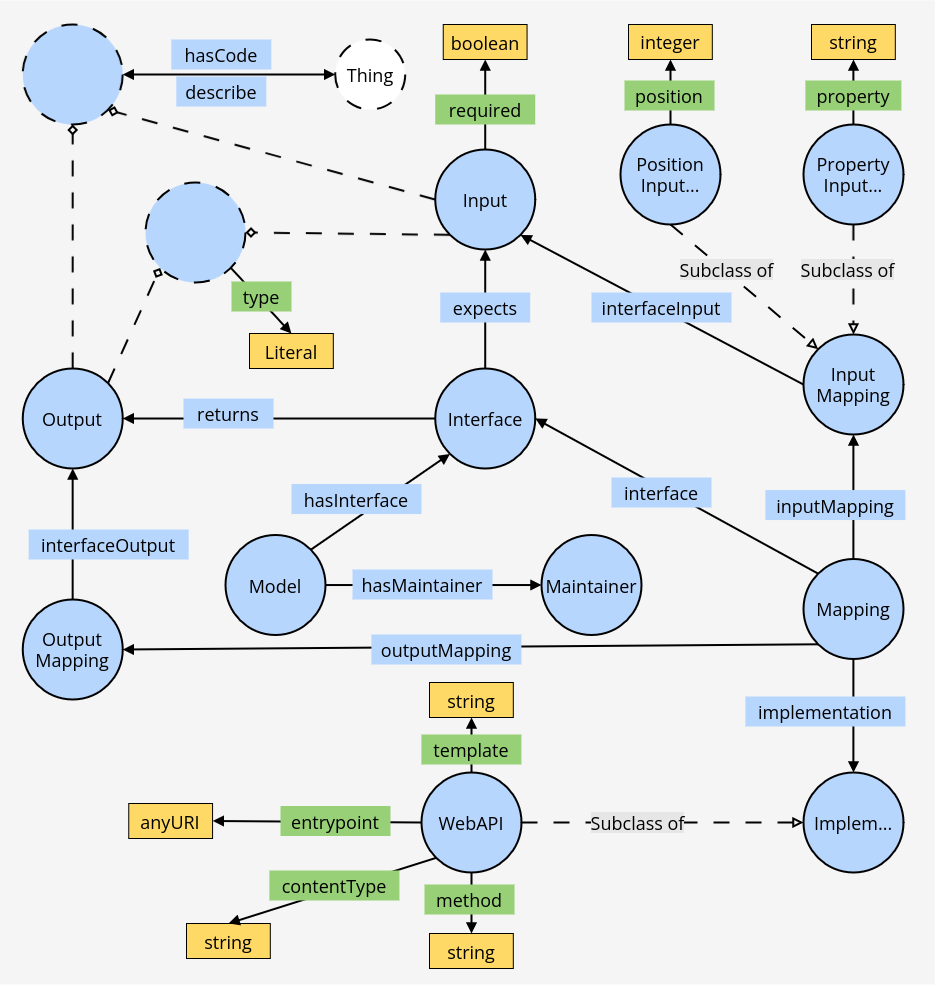
\includegraphics[width=1\linewidth]{figures/paper6/fig3.png}
    %%%% CHANGED: \caption{Visualization of the abstraction for the Model Interface Manifest Ontology.}\label{fig3}
    %%%% TO:
    \caption{MIMO ontology diagram illustrating OWL classes (blue circles), object properties (blue labels), and data properties (green labels), showing relationships among domain concepts. The ontology can be explored via \href{https://service.tib.eu/webvowl/\#iri=https://model-interface-manifest-ontology-ad0613.gitlab.io/MIMO.owl}{WebVOWL}.}\label{paper6_fig3}
\end{figure}

Logical validation was conducted using the Pellet Reasoner Plug-in (v2.2.0) within the Protégé environment. The reasoning process revealed no inconsistencies, affirming the ontology’s logical soundness and internal coherence. Furthermore, to evaluate MIMO's quality, we employed KGHeartBeat~\cite{pellegrino_kgheartbeat_2025}, a fully automated framework for KG quality assessment. It utilizes the \textit{Weighted Dimension Value} approach~\cite{debattista_luzzumethodology_2016} to produce normalized scores (0--100) across a broad spectrum of quality dimensions.
This methodology facilitates both fine-grained evaluation and holistic comparison.

The evaluation framework is grounded in the model proposed by Zaveri et al.~\cite{zaveri_2015}, which organizes quality assessment into 20 distinct dimensions, grouped under six dimension clusters:
\begin{itemize}
    \item \textit{Accessibility}: Pertains to data availability, licensing, interlinking, security, and performance aspects, all critical for reliable and authorized access.
    \item \textit{Intrinsic}: Focuses on context-independent features such as semantic accuracy, consistency, and conciseness, ensuring syntactic and logical integrity.
    \item \textit{Contextual}: Encompasses task-dependent metrics, with sub-clusters including:
    \begin{itemize}
        \item \textit{Trust}: Measures believability, reputation, and verifiability.
        \item \textit{Dataset Dynamicity}: Addresses temporal aspects such as currency and timeliness.
    \end{itemize}
    \item \textit{Representational}: Assesses the design and usability of data structures, including representational conciseness, interoperability, interpretability, understandability, and versatility.
\end{itemize}
%
Table~\ref{tab:paper6_qualitymetrics} presents the quality scores for each dimension. MIMO achieved a normalized total score of 71.3/100, indicating a high-quality design, particularly in the \textit{Intrinsic} and \textit{Representational} categories, essential for semantic interoperability and the seamless integration of AI components.

The table shows zero scores for metrics assessing links between MIMO and other ontologies. This applies to the Interlinking score, which evaluates alignment with other KGs; the Reputation score, derived from the PageRank algorithm to measure how many external graphs link to MIMO; and the Completeness score, which represents the ratio between triples with external links and the total triples of MIMO. This is because it is the first version of the ontology, which initially needs to support the integration of models into the platform. This basic operability is achieved without link MIMO to external knowledge graphs.

\begin{table}[ht]
\centering
%%%% CHANGED:
% \caption{KGHeartBeat Quality Metrics for MIMO by Dimension (Normalized 0--100)}
%%%% TO:
\caption{MIMO ontology quality scores computed with KGHeartBeat~\cite{pellegrino_kgheartbeat_2025}, following the methodology described in the \href{https://isislab-unisa.github.io/KGHeartBeat/}{official documentation}.}
\label{tab:paper6_qualitymetrics}
\begin{tabular*}{\tblwidth}{@{}LLC@{}}
\toprule
\textbf{Macro-group} & \textbf{Quality Dimension} & \textbf{Score} \\
\midrule
\multirow{5}{*}{Accessibility} 
  & Availability & 0.95 \\
  & Licensing & 1.00 \\
  & Interlinking & 0.00 \\
  & Security & 0.50 \\
  & Performance & 1.00 \\
\midrule
\multirow{3}{*}{Intrinsic} 
  & Semantic Accuracy & 1.00 \\
  & Consistency & 0.51 \\
  & Conciseness & 0.99 \\
\midrule
\multirow{3}{*}{Trust} 
  & Reputation & 0.00 \\
  & Believability & 0.75 \\
  & Verifiability & 0.99 \\
\midrule
\multirow{2}{*}{Dataset Dynamicity} 
  & Currency & 1.00 \\
  & Timeliness & 1.00 \\
\midrule
\multirow{2}{*}{Contextual} 
  & Completeness & 0.00 \\
  & Amount of Data & 1.00 \\
\midrule
\multirow{5}{*}{Representational} 
  & Representational Conciseness & 0.50 \\
  & Interoperability & 0.99\\
  & Understandability & 0.05  \\
  & Interpretability & 1.00 \\
  & Versatility & 1.00 \\
\midrule
\multicolumn{2}{l}{\textbf{Total Quality Score}} & \textbf{71.3} \\
\bottomrule
\end{tabular*}
\end{table}

%%%% CHANGED:
%\subsection{Test Manifest Protocol: Identifying High-risk Stroke Patients}
%%%% TO:
\subsubsection{Use Case: Stroke Risk Prediction}
A core innovation of the CONNECTED framework is its Manifest protocol. It enhances DTs with predictive capabilities through AI model integration. This protocol facilitates the seamless adaptation of general-purpose models to individual patients by incorporating historical and real-time clinical data. As a result, DTs can perform context-aware simulations with minimal manual configuration.

To test this mechanism, we implemented a use case focused on identifying patients at high risk of stroke. We integrated a Neural Network developed by Dev et al.~\cite{dev_predictive_2022}. It classifies stroke risk based on four key clinical features: age, average glucose level, hypertension status, and heart disease. The model was trained and evaluated using the dataset published in their public GitHub repository\footnote{\url{https://github.com/Soumyabrata/EHR-features}}, which includes 1,096 records—balanced between 548 stroke-positive and 548 stroke-negative patients. Following the original study, the dataset was split into training and testing sets using a 70:30 ratio, resulting in 329 test samples for performance evaluation.

We integrated the Neural Network within CONNECTED by defining a dedicated Manifest describing its structure, inputs, and expected outputs. This enabled its automated invocation via the Capabilities service, with patient data dynamically matched to the model’s input requirements. The resulting classification metrics from the Manifest-driven execution were compared against the original implementation to assess functional equivalence. The experimental setup and performance outcomes are detailed in the subsequent sections.

We follow the spirit of reproducible research, and therefore the created manifests, the models, and the code developed to realize this test and the proof-of-concept are available online\footnote{\url{https://gitlab.com/unibo-connected/connected-test}}.

\paragraph{Setup}
A total of 329 patients from the stroke classifier dataset~\cite{dev_predictive_2022} were used for simulation. For each patient, a DT was instantiated within the framework and populated with FHIR-based resources representing the four input features required by the model. These resources were further enriched with semantic annotations, including ontology references from standards such as LOINC and SNOMED-CT.

A Manifest describing the Neural Network was defined according to the MIMO ontology. This specification includes the model’s input parameters, API endpoint, expected data format, and execution constraints. The Manifest was uploaded to CONNECTED via the Manifest service and programmatically linked to the relevant DTs using the Capabilities service. Leveraging the framework’s data-to-model mechanism, all 329 DTs were automatically enhanced with stroke risk prediction capabilities.
%
\paragraph{Data Fusion and Semantic Integration}
For each DT, stroke risk prediction was initiated by invoking its associated capability. This process succeeds only if the DT contains sufficient data to satisfy the model’s input requirements: age, average glucose level, hypertension status, and heart disease. CONNECTED performs this validation automatically by extracting and combining three KGs: the Manifest, the Properties, and the current State of the DT. These graphs are then merged with domain ontologies (FHIR, MIMO, and SIMO) and passed to a Jena reasoner for semantic inference.

As illustrated in Figure~\ref{paper6_fig4}, the reasoner applies OWL-based description logic rules to infer semantic correspondences. Specifically, it establishes \texttt{canBeFulfilled} relationships between model input requirements and patient data nodes. The capability is deemed executable when the reasoner infers at least a link for each input.
%
\begin{figure*}
\centerline{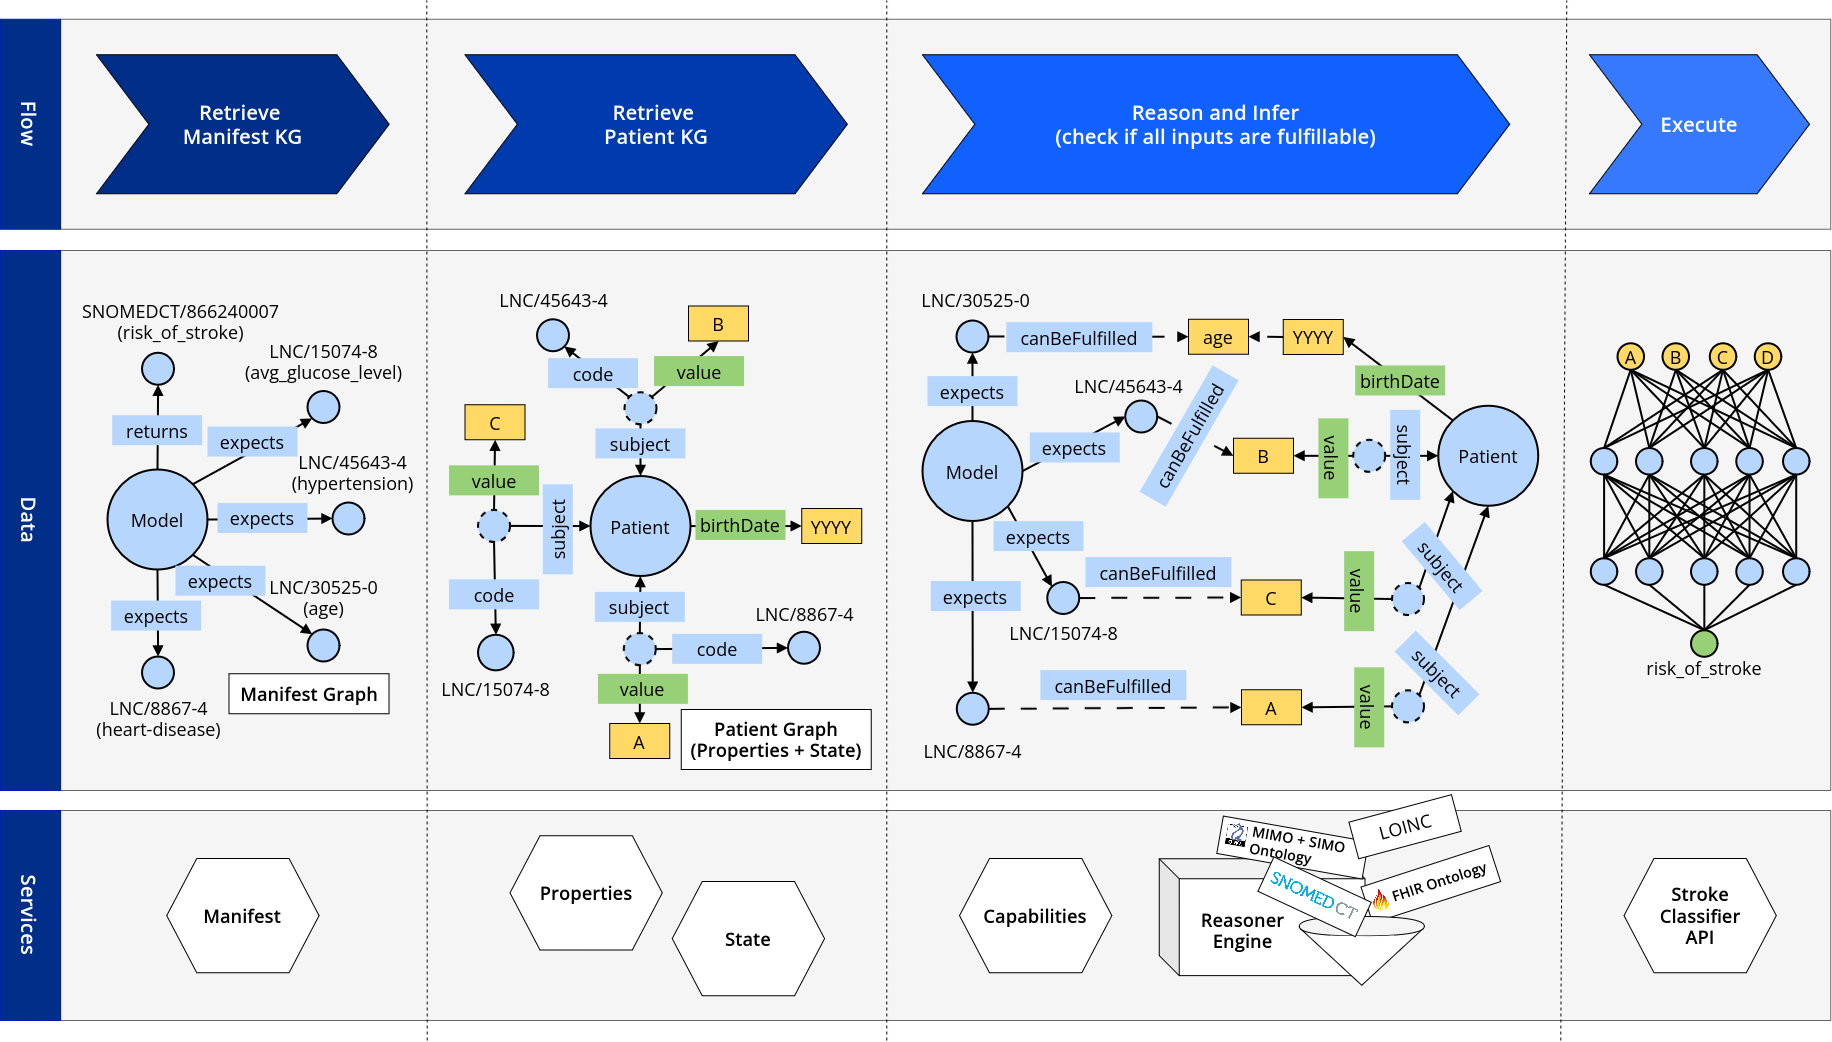
\includegraphics[width=\linewidth]{figures/paper6/fig4.png}}
\caption{Overview of the reasoning process aligning patient data with the stroke risk classifier’s input requirements.}
\label{paper6_fig4}
\end{figure*}
%
\paragraph{Simulation and Results Delivery}
As expected, CONNECTED’s internal data-model binding process matched all model inputs with corresponding patient information. Upon completion of semantic reasoning, the platform triggered the ML model by sending a properly formatted request to its API, as specified in the Manifest. The model’s binary prediction—indicating stroke risk—was then returned asynchronously via a WebSocket interface to the client application.

To validate correct integration, we compared the stroke risk predictions produced through Manifest-driven execution within CONNECTED against those generated by the original standalone Neural Network. Table~\ref{tab:paper6_model_comparison} shows that the evaluation metrics were identical across implementations. This confirms functional equivalence and demonstrates that the reasoning process does not introduce distortion or loss in predictive performance.

\begin{table}[ht]
\centering
\caption{Comparison of Neural Network performance metrics between standalone implementation and Manifest-driven execution in CONNECTED}
\label{tab:paper6_model_comparison}
\begin{tabular*}{\tblwidth}{@{}LCC@{}}
\toprule
\textbf{Metric} & \textbf{Standalone NN} & \textbf{CONNECTED Execution} \\
\midrule
Precision       & 0.74 & 0.74 \\
Recall          & 0.85 & 0.85 \\
F1-Score        & 0.79 & 0.79 \\
Accuracy        & 0.78 & 0.78 \\
Miss Rate       & 0.09 & 0.09 \\
Fall-out Rate   & 0.30 & 0.30 \\
\bottomrule
\end{tabular*}
\end{table}

%This highlights DT platforms’ potential to deliver personalized insights, identify high-risk patients, and support clinical decision-making. By integrating ML models, CONNECTED establishes a scalable approach for predictive healthcare, paving the way for diverse future applications.

%%%% CHANGED:
%\subsection{Application Use Case: A Proof-of-Concept for Model Benchmarking}
%%%% TO:
\subsubsection{Proof-of-Concept Benchmarking Application}
To further demonstrate the model-agnostic capabilities of the Manifest protocol and the practical utility of CONNECTED, we developed a proof-of-concept benchmarking application located at the Application Layer of the architecture. This application interacts with DTs via the framework's RESTful APIs and illustrates how diverse AI models can be semantically integrated, invoked, and evaluated through a uniform interface.

In this use case, we incorporated two additional stroke classifiers—Random Forest and Decision Tree—from Dev et al.’s study~\cite{dev_predictive_2022}, alongside the previously validated Neural Network. Each model was described using a distinct Manifest, detailing its input requirements, API endpoint, and constraints according to the MIMO ontology. These Manifests were uploaded to CONNECTED and linked to the DTs as new executable capabilities.

%%%% CHANGED:
%We designed an incremental evaluation strategy to emulate the gradual accumulation of data in real-world deployments. The 329 test patients were partitioned into ten sequential subsets (or “chunks”), progressively expanding the evaluation set by 10\% increments at each stage (e.g., 10\%, 20\%, ..., 100\%). Importantly, the models were not retrained or fine-tuned during this process; they remained static, enabling us to observe how their pretrained performance generalizes as new patient data is introduced. Specifically, we computed standard classification metrics (accuracy, precision, recall, and F1-score) after each evaluation set expansion. 

%This evaluation highlights not only static performance but also the robustness of each model, which is essential in clinical settings where decisions must often be made with limited initial data. As shown in Table~\ref{tab:benchmarking-metrics} and illustrated in Figure~\ref{fig:benchmarking-results}, performance variability is more pronounced in the early stages due to limited sample sizes. However, metrics stabilize as more patient data is incorporated, revealing each model’s robustness under evolving data conditions. Once stabilized, the Neural Network consistently achieved the highest performance among the tested models, confirming prior findings reported in Dev et al.~\cite{dev_predictive_2022}.
%%%% TO:
We designed an incremental evaluation strategy to emulate the gradual accumulation of patients in real-world deployments. In this work a test patient denotes a full patient-level record containing all available information for a single individual (demographics and the clinical features required by the models). The 329 patient-level records were partitioned into ten non-overlapping subsets (chunks) and the models were evaluated on the cumulative union of these chunks: stage $k$ uses the first $k$ chunks (10\%, 20\%, \dots, 100\% of the patients). Chunking was performed via stratified sampling to preserve the original stroke / non-stroke class ratio in each chunk, and the split is deterministic (fixed random seed) to ensure reproducibility. Chunk sizes are 33 patients for chunks 1–9 and 32 patients for chunk 10 (total 329). Importantly, models were kept static (no retraining or fine-tuning) between stages so that each stage measures how pretrained models generalize as new, distinct patients are introduced.

This incremental evaluation highlights not only static performance but also model robustness when operating with limited cohorts—an important property in clinical settings where decisions are often required early in deployment. After each cumulative expansion we computed standard classification metrics (accuracy, precision, recall, and F1-score) and report mean and dispersion (standard deviation and 95\% confidence intervals) across repeated runs. As shown in Table~\ref{tab:paper6_benchmarking-metrics} and Figure~\ref{fig:paper6_benchmarking-results}, performance variability is larger in early stages due to small sample sizes and stabilizes as more patient-level records are incorporated; once stabilized, the Neural Network consistently attains the highest performance among the tested models, in agreement with Dev et al.~\cite{dev_predictive_2022}. 

\begin{table*}[ht]
\centering
%%%% CHANGED:   
% \caption{Incremental evaluation of model performance over 10 cumulative patient data chunks. Metrics: Accuracy, Precision, Recall, and F1-score, reported for Neural Network (NN), Random Forest (RF), and Decision Tree (DT).}
%%%% TO:
\caption{Accuracy trends for Neural Network (NN), Random Forest (RF), and Decision Tree (DT) evaluated on cumulative patient-level test sets. The 329 patient-level records were partitioned into ten non-overlapping, stratified chunks.}
\label{tab:paper6_benchmarking-metrics}
\renewcommand{\arraystretch}{1.2}
\resizebox{\textwidth}{!}{% layout: resized to the thesis text width
\begin{tabular}{|c|c|ccc|ccc|ccc|ccc|}
\hline
\multirow{2}{*}{\textbf{Chunk}} & \multirow{2}{*}{\textbf{N}} & \multicolumn{3}{c|}{\textbf{Accuracy}} & \multicolumn{3}{c|}{\textbf{Precision}} & \multicolumn{3}{c|}{\textbf{Recall}} & \multicolumn{3}{c|}{\textbf{F1-score}} \\
\cline{3-14}
 &  & \textbf{NN} & \textbf{RF} & \textbf{DT} & \textbf{NN} & \textbf{RF} & \textbf{DT} & \textbf{NN} & \textbf{RF} & \textbf{DT} & \textbf{NN} & \textbf{RF} & \textbf{DT} \\
\hline
1  & 33  & 0.76 & 0.82 & 0.70 & 0.78 & 0.89 & 0.79 & 0.86 & 0.81 & 0.71 & 0.82 & 0.85 & 0.75 \\
2  & 66  & 0.77 & 0.79 & 0.71 & 0.78 & 0.84 & 0.78 & 0.88 & 0.80 & 0.72 & 0.82 & 0.82 & 0.75 \\
3  & 99  & 0.79 & 0.76 & 0.69 & 0.78 & 0.81 & 0.74 & 0.88 & 0.75 & 0.70 & 0.82 & 0.78 & 0.72 \\
4  & 132 & 0.80 & 0.73 & 0.68 & 0.81 & 0.80 & 0.76 & 0.86 & 0.73 & 0.68 & 0.83 & 0.77 & 0.72 \\
5  & 165 & 0.79 & 0.75 & 0.67 & 0.78 & 0.78 & 0.72 & 0.87 & 0.73 & 0.64 & 0.82 & 0.76 & 0.68 \\
6  & 198 & 0.79 & 0.74 & 0.67 & 0.75 & 0.76 & 0.69 & 0.87 & 0.73 & 0.62 & 0.81 & 0.74 & 0.66 \\
7  & 231 & 0.79 & 0.75 & 0.67 & 0.77 & 0.78 & 0.70 & 0.87 & 0.74 & 0.63 & 0.81 & 0.76 & 0.66 \\
8  & 264 & 0.78 & 0.75 & 0.66 & 0.75 & 0.75 & 0.68 & 0.85 & 0.76 & 0.64 & 0.80 & 0.75 & 0.66 \\
9  & 296 & 0.78 & 0.74 & 0.66 & 0.74 & 0.73 & 0.67 & 0.85 & 0.75 & 0.64 & 0.79 & 0.74 & 0.66 \\
10 & 329 & 0.78 & 0.74 & 0.66 & 0.74 & 0.73 & 0.66 & 0.85 & 0.76 & 0.65 & 0.79 & 0.74 & 0.66 \\
\hline
\end{tabular}
}
\end{table*}

\begin{figure}
\centerline{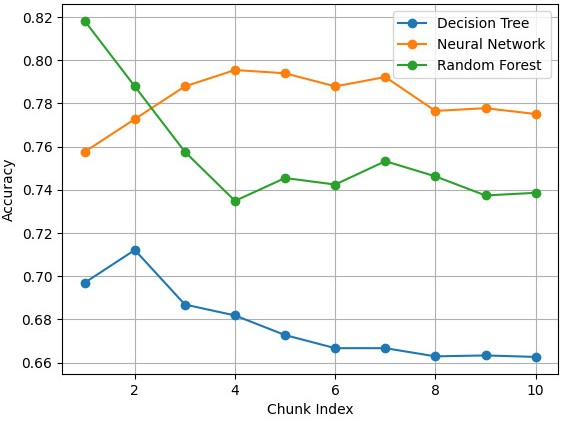
\includegraphics[width=\linewidth]{figures/paper6/fig8.jpeg}}
%%%% CHANGED:
% \caption{Accuracy trends for Neural Network, Decision Tree, and Random Forest models as the evaluation set incrementally increases.}
%%%% TO:
\caption{Accuracy trends for Decision Tree (DT), Neural Network (NN), and Random Forest (RF) as the evaluation set grows. Each point is computed on a cumulative patient-level set formed by sequentially adding non-overlapping patient groups (stage~1: $\approx$33 patients; stage~10: 329).}
\label{fig:paper6_benchmarking-results}
\end{figure}

Beyond benchmarking, this experiment underscores a broader capability of the framework: acting as a dynamic, semantically harmonized repository of patient-specific data. By continuously aggregating up-to-date clinical information into structured FHIR-based representations, CONNECTED enables ongoing validation of AI models under realistic and evolving conditions. As healthcare data streams from diverse sources, the system can support longitudinal model assessments, detect performance drift, and assist in model lifecycle monitoring—crucial elements for deploying safe and reliable AI in healthcare.

Moreover, the framework's semantic mediation and Manifest-driven execution architecture ensure that models can be assessed uniformly, regardless of their internal implementation or origin. This decoupling of models from data infrastructure reinforces CONNECTED's role as a testbed for adaptive deployment strategies in clinical environments.
%
%%%% CHANGED:
%%%% TO:
\subsubsection{Performance Evaluation}\label{sec:paper6_performance}
This section evaluates the performance of the CONNECTED platform in terms of scalability, latency, and throughput under varying levels of concurrent load. The aim is to provide concrete evidence of the platform's computational footprint and responsiveness in realistic deployment conditions, identify likely bottlenecks, and offer guidance on minimum and recommended system requirements for small- to medium-scale use.

All experiments were executed on a single-host deployment running the full CONNECTED application stack inside Docker containers. The host machine used for the experiments was equipped with an AMD Ryzen~5~5600X (6 physical cores), 16\,GB of RAM, and Ubuntu~24.04~LTS; Docker~24.0+ and Docker~Compose~2.20+ were used to orchestrate the containers, and Python~3.10+ was used for benchmarking. To inform prospective adopters, we recommend a minimum baseline configuration of a 4-core CPU, 8\,GB RAM, and 10\,GB of available disk for modest, single-host deployments; for moderate production usage, we recommend a 6-core CPU and 16\,GB RAM (the configuration used in our tests). During the heaviest tested load (20 concurrent threads), the host’s average memory consumption was approximately 2.8\,GB, indicating a modest memory footprint for the evaluated scenario.

Workload generation and measurement were performed using a custom Python profiling script that employs a \texttt{ThreadPoolExecutor} to issue concurrent HTTP prediction requests against the platform’s REST API. Each request executed a complete digital-twin simulation for a single patient and returned the corresponding prediction. Each experimental run issued 329 independent requests (matching the evaluation dataset); no caching or shared state was used between requests. We exercised four concurrency levels (1, 5, 10, and 20 worker threads) and collected per-request response traces from which we derived mean and median latency (ms), 95th-percentile latency (p95, ms), and throughput (successful requests per second, req/s).

Table~\ref{tab:paper6_performance} summarizes the measured metrics across all concurrency levels. As concurrency increases, overall throughput rises substantially, from 5.4\,req/s at a single thread to 26.7\,req/s at 20 threads. However, this improvement is accompanied by a gradual increase in latency: the mean latency grows from 185\,ms (1 thread) to 737\,ms (20 threads), and the 95th percentile latency reaches approximately 912\,ms.
\begin{table*}[ht]
\centering
\caption{Performance metrics across different concurrency levels.}
\label{tab:paper6_performance}
\resizebox{\textwidth}{!}{% layout: resized to the thesis text width
\begin{tabular}{c c c c c}
\toprule
\textbf{Concurrency} & \textbf{Mean (ms)} & \textbf{Median (ms)} & \textbf{p95 (ms)} & \textbf{Throughput (req/s)} \\
\midrule
1  & 184.98 & 182.05 & 204.11 & 5.41 \\
5  & 242.19 & 240.20 & 286.58 & 20.48 \\
10 & 385.98 & 382.64 & 467.93 & 25.70 \\
20 & 736.90 & 745.12 & 912.40 & 26.71 \\
\bottomrule
\end{tabular}
}
\end{table*}
%
Figure~\ref{fig:paper6_performance_plots} provides a visual summary of the performance behavior. The latency cumulative distribution (Figure~\ref{fig:paper6_latency_cdf}) shows that, in sequential execution, most requests complete within 200\,ms, indicating a low base latency under minimal contention. The throughput plot (Figure~\ref{fig:paper6_throughput}) highlights the scalability of the platform: throughput grows almost linearly up to 10 concurrent threads before plateauing near 26\,req/s. This behavior suggests that the system effectively utilizes available CPU cores up to a certain point, after which contention and scheduling overheads limit further gains. The 95th percentile latency (Figure~\ref{fig:paper6_p95_latency}) exhibits a similar pattern, increasing sharply beyond 10 threads due to resource competition among containers.
%
\begin{figure*}[t]
    \centering
    % Subfigure 1
    \begin{subfigure}{0.32\linewidth}
        \centering
        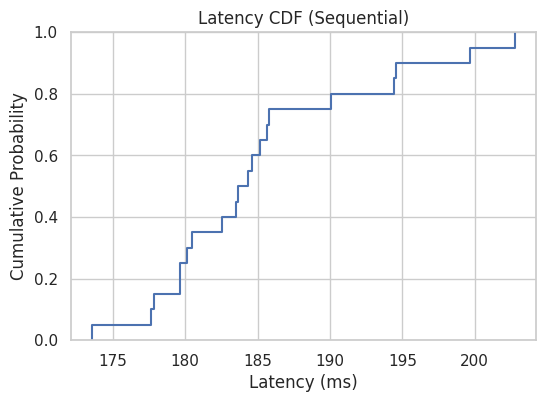
\includegraphics[width=\linewidth]{figures/paper6/fig9.png}
        \caption{Latency CDF (Sequential)}
        \label{fig:paper6_latency_cdf}
    \end{subfigure}
    \hfill
    % Subfigure 2
    \begin{subfigure}{0.32\linewidth}
        \centering
        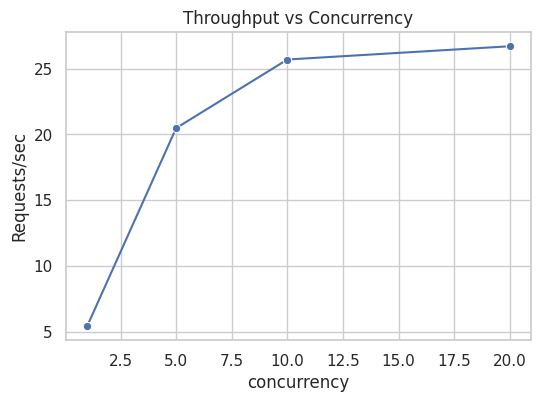
\includegraphics[width=\linewidth]{figures/paper6/fig10.png}
        \caption{Throughput vs Concurrency}
        \label{fig:paper6_throughput}
    \end{subfigure}
    \hfill
    % Subfigure 3
    \begin{subfigure}{0.32\linewidth}
        \centering
        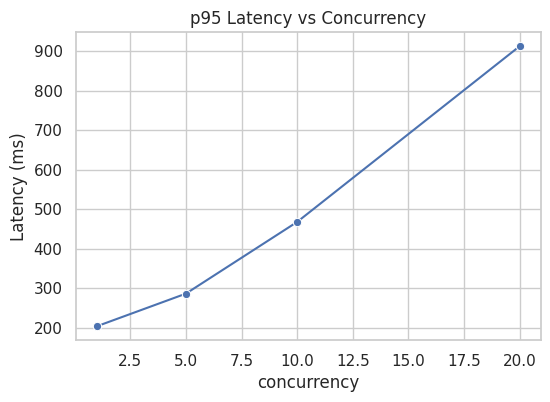
\includegraphics[width=\linewidth]{figures/paper6/fig11.png}
        \caption{95th Percentile Latency vs Concurrency}
        \label{fig:paper6_p95_latency}
    \end{subfigure}
    %
    \caption{
        Performance evaluation of the CONNECTED platform.
        (a) Cumulative distribution of request latency for sequential execution.
        (b) Throughput scaling with increasing concurrency levels.
        (c) Variation of the 95th percentile latency with concurrency.
    }
    \label{fig:paper6_performance_plots}
\end{figure*}
Overall, these results demonstrate that the CONNECTED platform scales efficiently up to moderate levels of concurrency while maintaining acceptable response times. The observed throughput–latency tradeoff is consistent with the expected behavior of containerized, compute-intensive workloads.
\subsection{Discussion}~\label{sec:paper6_discussion}
This work presented a preliminary implementation of the CONNECTED framework, demonstrating its effectiveness in supporting the deployment of semantically enriched, AI-powered DTs for healthcare applications. The platform is designed to predict future patient trajectories while promoting semantic interoperability, model transparency, and automation of model integration through Semantic Web technologies.

Our core contributions include: (1) the development of a FHIR-compliant, patient-centric API (DT Layer) that enables structured access to clinical histories, real-time health monitoring, and simulation of future states; (2) the publication of MIMO within the LOD Cloud, facilitating transparent, standards-based model interface descriptions; (3) the implementation of the Manifest protocol to automate data-to-model binding, thereby enabling seamless integration of AI models tailored to individual patient profiles; and (4) a proof-of-concept benchmarking application that continuously evaluates and ranks stroke risk classifiers in real time, driven by streaming patient data.

A key strength of CONNECTED lies in its modular, microservice-based architecture, which promotes scalability, flexibility, and ease of maintenance. The ability to dynamically integrate AI models through declarative manifests enables the system to adapt to new clinical domains and use cases. Furthermore, the semantic infrastructure powered by ontologies and KGs supports standardized model descriptions and rich patient representations, improving interpretability and reuse.
%
\subsubsection{Challenges and Limitations}
Despite its promise, the CONNECTED framework faces several limitations that must be addressed to achieve broader real-world applicability. First, the platform lacks substantial engagement from key stakeholders, including healthcare professionals, domain experts, and patients. This gap hinders the validation of its practical utility and the alignment of services with clinical needs. Moreover, its expressivity has been tested only within a controlled use case, limiting generalizability to diverse healthcare scenarios.

Technically, the current implementation of the Application Layer is emulated through a REST client and is not driven by end-user requirements. Future developments require stakeholder collaboration to design services that better meet clinical needs. Additionally, the platform's support for a patient-centered care model remains limited.

Privacy and security pose significant challenges, particularly given the sensitive nature of health data. Ensuring compliance with data protection regulations and implementing robust safeguards are imperative~\cite{jawad_security_2024}. Socio-ethical concerns—including algorithmic bias, legal uncertainties, and the high cost of implementation—also pose risks to adoption and may exacerbate existing disparities in healthcare delivery~\cite{Katsoulakis2024}.

From a systems perspective, the implemented framework assumes the availability of clean, reliable, and harmonized data from the Source Layer. This assumption is often unrealistic due to the heterogeneity and fragmentation of healthcare data systems. Furthermore, CONNECTED lacks a coherent strategy for historical data management, including decisions about long-term storage and appropriate technologies.

The platform employs a synchronous communication pattern that may become a bottleneck in high-throughput environments, raising scalability concerns. The platform also lacks well-defined authorization mechanisms (e.g., Role-Based Access Control), introducing potential security vulnerabilities. Additionally, the inability of individual Digital Twins to collaborate restricts the platform’s analytical potential, while the symbolic AI components, especially those facilitating explainability, are underutilized.

Finally, the assumption that each model independently handles data preprocessing can hinder integration, especially for models with stringent input requirements or dependencies.

\subsubsection{Future Research}
Future research will prioritize enhancing stakeholder engagement, technical scalability, and clinical usability. A clinician dashboard will be developed to support the orchestration and analysis of DTs, enabling users to manage patient profiles, simulate health trajectories over varying time frames, and compare predicted outcomes. Moreover, we will realize an intelligent assistant that interacts with individual patient twins to enhance engagement by offering proactive insights, alerts, and access to clinical histories.

On the technical front, robust and flexible data ingestion mechanisms are critical. This includes the adoption of communication middleware (e.g., Eclipse Hono) to support protocol translation, proprietary-to-FHIR mappings, and asynchronous data flows. Strategies like ETL pipelines, data aggregation, and distributed database replication will be explored to accommodate the growing volume of patient data.

The communication architecture should shift toward an asynchronous, event-driven model to support higher scalability and resilience. Establishing a standard workflow framework for data preprocessing will also be essential, enabling broader compatibility with diverse AI models. Additionally, enabling model pipelines—where the output of one model serves as input to another—will allow the definition of compound capabilities and support multi-stage analyses.

A pivotal direction for future work is the integration of Collective Digital Twins (CDTs), representing patient cohorts rather than individuals. This population-level abstraction will enable cohort-based analysis (e.g., filtering by age, diagnosis, or risk factors) and serve as a harmonized data source for training and validating AI models. This shift also introduces the opportunity to support model development, not just model deployment, thereby enabling the integration of MLOps principles into the CONNECTED pipeline.

The evolution of MIMO is central to this vision. It will be extended to describe model-related metadata such as performance metrics, training datasets, licensing terms, ethical considerations, and data sensitivity. To this end, we plan to align MIMO with the Model Card Report Ontology (MCRO)~\cite{Amith2022}, enhancing transparency and responsible AI practices.

An additional extension of MIMO will support the composition of model interfaces. Given formal descriptions of model inputs and outputs, it becomes feasible to orchestrate multi-model pipelines where intermediate outputs serve as inputs for subsequent models, thus enabling composite DT capabilities and more insightful analysis.

Finally, leveraging the patient-centric KG will further enrich CONNECTED's potential. The KG can be augmented via link prediction to infer missing relations and support reasoning over incomplete data. This future extension would also enhance explainability by connecting AI predictions to clinically accepted ontologies, offering interpretable pathways for decision support. In addition, the KG enables exploratory search, helping clinicians and researchers uncover hidden patterns and draw deeper insights from patient-specific data.

These research directions will reinforce CONNECTED’s role as a general-purpose framework for deploying AI-powered patient DTs. In particular, these extensions will enhance its adaptability to the evolving healthcare landscape, supporting the development of intelligent, insight-driven applications that respond to the dynamic needs of both patients and providers.

\subsection*{Code Availability}
The CONNECTED code is available from the corresponding author upon reasonable request. MIMO is publicly accessible in the LOD Cloud at \url{https://lod-cloud.net/dataset/CONNECTED}, with OWL documentation provided at \url{https://model-interface-manifest-ontology-ad0613.gitlab.io/}. All artifacts related to the Manifest protocol evaluation and the benchmarking proof-of-concept—including manifests, AI models, and supporting code—are openly available at: 
\url{https://gitlab.com/unibo-connected/connected-test}

\subsection*{Acknowledgment}
This study was partially supported by the Italian Ministry of University and Research under PNRR-PNC Project PNC0000002 ”DARE – Digital Lifelong Prevention” (CUP: B53C22006450001).

% layout: keep this paper's floats within its section
\FloatBarrier




%----------------------------------------------------------------------------------------

% \sidenote{Add sidenotes in this way. They are named after the author of the thesis}

% %\paragraph{Structure of the Thesis}

% \note{Racall to describe the structure of the paper}

% \part{First Part}

% \chapter{State of the art}

% I suggest referencing stuff as follows: \cref{fig:random-image} or \Cref{fig:random-image}

% \begin{figure}
%     \centering
%     \includegraphics[width=.8\linewidth]{figures/random-image.pdf}
%     \caption{Some random image}
%     \label{fig:random-image}
% \end{figure}

% \section{Some cool topic}

% \part{Second Part}

% \chapter{Contribution}

% You may also put some code snippet (which is NOT float by default), eg: \cref{lst:random-code}.

% \lstinputlisting[float,language=Java,label={lst:random-code}]{listings/HelloWorld.java}

% \section{Fancy formulas here}

%----------------------------------------------------------------------------------------
% BIBLIOGRAPHY
%----------------------------------------------------------------------------------------

\backmatter

\part*{}

\nocite{*} % comment this to only show the referenced entries from the .bib file
\bibliographystyle{alpha}
\bibliography{phd-thesis}

\end{document}
